% !TeX document-id = {639a1635-118c-435b-a520-0a3fffad3c3f}
% !TeX program = xelatex
% !TeX encoding = UTF-8
% Main LaTeX file for the QRTable undergraduate thesis.
% Build from this directory with: xelatex undergraduate-theses-report.tex
\ifdefined\ThesisDuplex
  \documentclass[12pt,a4paper,twoside,openany]{report}
\else
  \documentclass[12pt,a4paper,oneside]{report}
\fi

\usepackage{iftex}
\ifPDFTeX
  \errmessage{This thesis template requires XeTeX/LuaTeX. Use Tectonic, XeLaTeX, or LuaLaTeX.}
\fi

\usepackage{fontspec}
\IfFontExistsTF{Times New Roman}{%
  \setmainfont{Times New Roman}
}{%
  \setmainfont{TeX Gyre Termes}
}

\ifdefined\ThesisDuplex
  \usepackage[a4paper,top=3cm,bottom=3.5cm,inner=3.5cm,outer=2cm,headheight=14pt,footskip=1.2cm]{geometry}
\else
  \usepackage[a4paper,top=3cm,bottom=3.5cm,left=3.5cm,right=2cm,headheight=14pt,footskip=1.2cm]{geometry}
\fi
\usepackage{setspace}
\usepackage{fancyhdr}
\usepackage{titlesec}
\usepackage{tocloft}
\usepackage{caption}
\usepackage{array}
\usepackage{tabularx}
\usepackage{longtable}
\usepackage{booktabs}
\usepackage{csquotes}
\usepackage{xcolor}
\usepackage{graphicx}
\usepackage{svg}
\svgsetup{
  inkscapeversion=1.2.0,
  inkscapelatex=false,
  inkscapeexe={./tools/inkscape-rsvg-shim.sh},
}
\usepackage{float}
\usepackage[section]{placeins}
\usepackage{xurl}
\usepackage{hyperref}
\usepackage[
  backend=bibtex,
  style=ieee,
  sorting=nty
]{biblatex}

\BiblatexSplitbibDefernumbersWarningOff
\addbibresource{references.bib}
\AtEveryBibitem{%
  \clearfield{language}%
  \clearlist{language}%
}
\setcounter{biburlnumpenalty}{9000}
\setcounter{biburlucpenalty}{9000}
\setcounter{biburllcpenalty}{9000}

\hypersetup{
  unicode=true,
  hidelinks,
  pdftitle={Nghiên cứu và xây dựng nền tảng POS theo mô hình SaaS tích hợp đặt món qua mã QR dựa trên kiến trúc vi dịch vụ},
  pdfauthor={Vo Dinh Minh Quan}
}

\graphicspath{{assets/figures/}{assets/screenshots/}{assets/diagrams/}}
% Screenshot helpers for compact multi-column UI flows.
\newif\ifscreenshotplaceholder
\screenshotplaceholderfalse

\newcommand{\screenshotcaptionprefix}{%
  \ifscreenshotplaceholder
    [Minh họa tạm] %
  \fi
}
\newcommand{\screenshotcaptionsuffix}{%
  \ifscreenshotplaceholder
    \ Ảnh minh họa cần được thay bằng ảnh chụp client QRTable trước khi dùng làm hiện vật.%
  \fi
}

% Extra \label in same figure (shared figure number) — PWA grouped figures only
\newcommand{\screenshotgridanchor}[1]{\label{#1}}

% Management App — one screen per figure, full text width
\newcommand{\screenshotmgmtmaxheight}{0.62\textheight}
\newcommand{\screenshotmgmtcol}{0.48\linewidth}
\newcommand{\screenshotmgmtheight}{0.38\textheight}
\newcommand{\screenshotfiguremgmt}[3]{%
  \begin{figure}[htbp]%
    \centering%
    \includegraphics[width=\textwidth,height=\screenshotmgmtmaxheight,keepaspectratio]{#1}%
    \caption{\screenshotcaptionprefix #2\screenshotcaptionsuffix}%
    \label{#3}%
  \end{figure}%
}

% Customer PWA — minimal gutter; duo = 2 cols/row, triple = 3 cols/one row
\newlength{\screenshotpwathreecolwidth}
\newcommand{\screenshotpwagutterduo}{2pt}
\newcommand{\screenshotpwagutterthree}{0.5pt}
\newcommand{\screenshotpwacolwidthduo}{0.495\linewidth}
\newcommand{\screenshotpwaheightduo}{0.72\textheight}
\newcommand{\screenshotpwaheightthree}{0.78\textheight}
\newcommand{\screenshotpwacellduo}[1]{%
  \begin{minipage}[t]{\screenshotpwacolwidthduo}%
    \centering%
    \includegraphics[width=\linewidth,height=\screenshotpwaheightduo,keepaspectratio]{#1}%
  \end{minipage}%
}
\newcommand{\screenshotpwacellthree}[1]{%
  \begin{minipage}[t]{\screenshotpwathreecolwidth}%
    \centering%
    \includegraphics[width=\linewidth,height=\screenshotpwaheightthree,keepaspectratio]{#1}%
  \end{minipage}%
}
\newcommand{\screenshotpwafiguretwo}[4]{%
  \begin{figure}[H]%
    \centering%
    \setlength{\tabcolsep}{\screenshotpwagutterduo}%
    \renewcommand{\arraystretch}{1.0}%
    \begin{tabular}{@{}cc@{}}%
      \screenshotpwacellduo{#3} & \screenshotpwacellduo{#4} \\
    \end{tabular}%
    \caption{\screenshotcaptionprefix #1\screenshotcaptionsuffix}%
    \label{#2}%
  \end{figure}%
}
\newcommand{\screenshotpwafigurethree}[5]{%
  \begin{figure}[H]%
    \centering%
    \setlength{\tabcolsep}{\screenshotpwagutterthree}%
    \setlength{\screenshotpwathreecolwidth}{\dimexpr(\linewidth-4pt)/3\relax}%
    \renewcommand{\arraystretch}{1.0}%
    \begin{tabular}{@{}ccc@{}}%
      \screenshotpwacellthree{#3} & \screenshotpwacellthree{#4} & \screenshotpwacellthree{#5} \\
    \end{tabular}%
    \caption{\screenshotcaptionprefix #1\screenshotcaptionsuffix}%
    \label{#2}%
  \end{figure}%
}

% Compatibility helpers for appendix-generated screenshot grids.
\newcommand{\screenshotgridcell}[3]{%
  \begin{minipage}[t]{#1}%
    \centering%
    \includegraphics[width=\linewidth,height=#2,keepaspectratio]{#3}%
  \end{minipage}%
}
\newcommand{\chapterscreenshot}[3]{%
  \screenshotfiguremgmt{#1}{#2}{#3}%
}

\newcommand{\appendixscreenshot}[3]{%
  \begin{figure}[htbp]%
    \centering%
    \includegraphics[width=0.92\textwidth,height=0.38\textheight,keepaspectratio]{#1}%
    \caption{\screenshotcaptionprefix #2\screenshotcaptionsuffix}%
    \label{#3}%
  \end{figure}%
}

% --- Screenshot guide, hidden when \screenshotplaceholderfalse ---
\newcommand{\screenshotcaptureguide}[1]{%
  \ifscreenshotplaceholder
  \par\small
  \noindent\fbox{\begin{minipage}{\dimexpr\linewidth-2\fboxsep-2\fboxrule\relax}
  \textbf{Ghi chú hiện vật minh họa.}
  Lưu vào \texttt{thesis-report/assets/screenshots/} (đúng tên file, không đổi).
  Khi đã có ảnh thật, giữ \texttt{\textbackslash screenshotplaceholderfalse} trong \texttt{screenshot-scaffold.tex} để ẩn khối hướng dẫn này.
  \begin{itemize}\setlength{\itemsep}{2pt}\setlength{\parsep}{0pt}
  #1%
  \end{itemize}
  \end{minipage}}\par
  \fi
}
\newcommand{\screenshotcapturerow}[3]{%
  \item[\textbf{#1}] \texttt{#2} --- #3%
}


\makeatletter
\renewcommand\normalsize{\@setfontsize\normalsize{13pt}{19.5pt}}
\makeatother
\normalsize
\setlength{\parindent}{1.25cm}
\setlength{\parskip}{0pt}
\setcounter{secnumdepth}{3}
\setcounter{tocdepth}{3}

\renewcommand{\chaptername}{Chương}
\renewcommand{\contentsname}{MỤC LỤC}
\renewcommand{\listfigurename}{DANH MỤC HÌNH}
\renewcommand{\listtablename}{DANH MỤC BẢNG}
\renewcommand{\figurename}{Hình}
\renewcommand{\tablename}{Bảng}
\renewcommand{\bibname}{TÀI LIỆU THAM KHẢO}

\titleformat{\chapter}[hang]
  {\normalfont\bfseries\fontsize{14}{18}\selectfont}
  {\chaptername\ \thechapter.}
  {0.75em}
  {}
\titlespacing*{\chapter}{0pt}{0pt}{18pt}
\titleformat{\section}{\normalfont\bfseries\fontsize{13}{18}\selectfont}{\thesection.}{0.75em}{}
\titleformat{\subsection}{\normalfont\bfseries\fontsize{13}{18}\selectfont}{\thesubsection.}{0.75em}{}
\titleformat{\subsubsection}{\normalfont\bfseries\fontsize{13}{18}\selectfont}{\thesubsubsection.}{0.75em}{}

\captionsetup{font={stretch=1.5},labelfont=bf,labelsep=period}

\fancypagestyle{mainpages}{%
  \fancyhf{}%
  \renewcommand{\headrulewidth}{0pt}%
  \renewcommand{\footrulewidth}{0pt}%
  \fancyfoot[C]{\thepage}%
}

\newcommand{\thesistitle}{Nghiên cứu và xây dựng nền tảng POS theo mô hình SaaS tích hợp đặt món qua mã QR dựa trên kiến trúc vi dịch vụ}
\newcommand{\thesisenglishtitle}{Research on the Development of a SaaS-Based POS Platform Integrating QR Code Ordering under a Microservices Architecture}
\newcommand{\thesisauthor}{Võ Đình Minh Quân}
\newcommand{\thesisstudentid}{22521193}
\newcommand{\thesisfaculty}{KHOA HỆ THỐNG THÔNG TIN}
\newcommand{\thesismajor}{HỆ THỐNG THÔNG TIN}
\newcommand{\thesisdegree}{CỬ NHÂN}
\newcommand{\thesissupervisor}{TS. NGUYỄN THANH BÌNH}
\newcommand{\thesisyear}{2026}

\newcommand{\covergeometry}{\newgeometry{top=2cm,right=2cm,bottom=1.5cm,left=2.54cm,headheight=14pt,footskip=0.7cm}}
\ifdefined\ThesisDuplex
  \newcommand{\maingeometry}{\newgeometry{top=3cm,bottom=3.5cm,inner=3.5cm,outer=2cm,headheight=14pt,footskip=1.2cm}}
\else
  \newcommand{\maingeometry}{\newgeometry{top=3cm,bottom=3.5cm,left=3.5cm,right=2cm,headheight=14pt,footskip=1.2cm}}
\fi
\newcommand{\centerbold}[2]{{\centering\fontsize{#1}{#1}\selectfont\bfseries #2\par}}

\ifdefined\ThesisDuplex
  % Avoid stretching vertical gaps around large figures in the duplex build.
  \raggedbottom
\fi

\begin{document}

\pagenumbering{gobble}
\pagestyle{empty}
\covergeometry

\begin{titlepage}
\centering
\centerbold{14}{ĐẠI HỌC QUỐC GIA TP. HỒ CHÍ MINH}
\vspace{0.2cm}
\centerbold{16}{TRƯỜNG ĐẠI HỌC CÔNG NGHỆ THÔNG TIN}
\vspace{0.2cm}
\centerbold{16}{\thesisfaculty}

\vspace{3.2cm}
\centerbold{14}{\thesisauthor}

\vspace{3.0cm}
\centerbold{16}{KHÓA LUẬN TỐT NGHIỆP}
\vspace{0.5cm}
{\fontsize{18}{24}\selectfont\bfseries \thesistitle\par}
\vspace{0.5cm}
{\fontsize{15}{20}\selectfont\bfseries \thesisenglishtitle\par}

\vspace{1.4cm}
\centerbold{14}{\thesisdegree{} NGÀNH \thesismajor}

\vfill
\centerbold{13}{TP. HỒ CHÍ MINH, \thesisyear}
\end{titlepage}

\begin{titlepage}
\centering
\centerbold{14}{ĐẠI HỌC QUỐC GIA TP. HỒ CHÍ MINH}
\vspace{0.2cm}
\centerbold{16}{TRƯỜNG ĐẠI HỌC CÔNG NGHỆ THÔNG TIN}
\vspace{0.2cm}
\centerbold{16}{\thesisfaculty}

\vspace{2.8cm}
\centerbold{14}{\thesisauthor{} -- \thesisstudentid}

\vspace{2.8cm}
\centerbold{16}{KHÓA LUẬN TỐT NGHIỆP}
\vspace{0.5cm}
{\fontsize{18}{24}\selectfont\bfseries \thesistitle\par}
\vspace{0.5cm}
{\fontsize{15}{20}\selectfont\bfseries \thesisenglishtitle\par}

\vspace{1.2cm}
\centerbold{14}{\thesisdegree{} NGÀNH \thesismajor}

\vspace{1.8cm}
\centerbold{14}{GIẢNG VIÊN HƯỚNG DẪN}
\vspace{0.2cm}
\centerbold{14}{\thesissupervisor}

\vfill
\centerbold{13}{TP. HỒ CHÍ MINH, \thesisyear}
\end{titlepage}

\maingeometry

\ifdefined\ThesisDuplex
  \setcounter{page}{3}
\fi
\maingeometry
\chapter*{LỜI CẢM ƠN}

Trước hết, em xin bày tỏ lòng biết ơn sâu sắc đến TS. Nguyễn Thanh Bình, giảng viên hướng dẫn khóa luận tốt nghiệp của em. Trong quá trình thực hiện đề tài, Thầy đã dành thời gian định hướng, góp ý và giúp em nhìn nhận bài toán không chỉ ở góc độ xây dựng phần mềm, mà còn ở góc độ phân tích yêu cầu, thiết kế kiến trúc và đánh giá kết quả một cách có cơ sở. Những góp ý của Thầy là nền tảng quan trọng giúp em hoàn thiện dần nội dung nghiên cứu, hệ thống QRTable và bản báo cáo khóa luận này.

Em xin chân thành cảm ơn Ban Giám hiệu, Khoa Hệ thống Thông tin và quý Thầy, Cô Trường Đại học Công nghệ Thông tin, Đại học Quốc gia Thành phố Hồ Chí Minh đã tạo môi trường học tập, nghiên cứu và rèn luyện chuyên môn trong suốt thời gian em theo học tại trường. Các kiến thức về cơ sở dữ liệu, phân tích thiết kế hệ thống, kiến trúc phần mềm, phát triển ứng dụng và bảo đảm chất lượng phần mềm đã hỗ trợ trực tiếp cho quá trình thực hiện đề tài.

Em cũng xin gửi lời cảm ơn đến gia đình, người thân và bạn bè đã luôn động viên, chia sẻ và tạo điều kiện để em duy trì tinh thần học tập, nghiên cứu trong quá trình hoàn thành khóa luận. Sự đồng hành và khích lệ của mọi người là nguồn động lực lớn giúp em vượt qua những giai đoạn khó khăn khi triển khai hệ thống và hoàn thiện báo cáo.

Mặc dù đã cố gắng thực hiện đề tài một cách nghiêm túc, khóa luận khó tránh khỏi những thiếu sót do giới hạn về thời gian, kinh nghiệm và phạm vi triển khai. Em kính mong nhận được sự góp ý của quý Thầy, Cô để có thể tiếp tục hoàn thiện đề tài và phát triển hệ thống tốt hơn trong tương lai.

\begin{flushright}
TP. Hồ Chí Minh, tháng 6 năm 2026\\
\thesisauthor
\end{flushright}

\cleardoublepage


\cleardoublepage
\tableofcontents
\cleardoublepage
\listoffigures
\cleardoublepage
\listoftables
\cleardoublepage
\chapter*{DANH MỤC TỪ VIẾT TẮT}

\begin{longtable}{>{\bfseries}p{3cm}p{10cm}}
API & Application Programming Interface \\
BFF & Backend for Frontend \\
EDA & Event-Driven Architecture \\
F\&B & Food and Beverage \\
IAM & Identity and Access Management \\
JWT & JSON Web Token \\
KDS & Kitchen Display System \\
NFR & Non-Functional Requirement \\
OIDC & OpenID Connect \\
POS & Point of Sale \\
PWA & Progressive Web App \\
QR & Quick Response \\
RBAC & Role-Based Access Control \\
SaaS & Software as a Service \\
SLA & Service Level Agreement \\
SLO & Service Level Objective \\
UI & User Interface \\
VND & Vietnamese Dong \\
\end{longtable}

\cleardoublepage


\cleardoublepage
\pagenumbering{arabic}
\pagestyle{mainpages}
\chapter*{TÓM TẮT KHÓA LUẬN}
\addcontentsline{toc}{chapter}{TÓM TẮT KHÓA LUẬN}

Trong lĩnh vực nhà hàng và dịch vụ ăn uống (F\&B), quy trình phục vụ tại bàn thường liên quan đến nhiều nhóm tác nhân như khách hàng, nhân viên phục vụ, bếp, thu ngân, chủ cửa hàng và bộ phận quản trị. Khi số lượng bàn, món ăn, đơn hàng và hình thức thanh toán tăng lên, cách vận hành thủ công hoặc các hệ thống bán hàng POS đơn lẻ dễ gặp khó khăn trong việc đồng bộ trạng thái đơn, kiểm soát tồn kho, cập nhật bếp, quản lý nhiều chi nhánh/đơn vị thuê bao và tích hợp thanh toán điện tử. Bên cạnh đó, mô hình đặt món qua mã QR giúp khách hàng thao tác trực tiếp trên thiết bị cá nhân, nhưng cũng đặt ra yêu cầu mới về xác thực phiên tại bàn, chống gửi trùng đơn, phối hợp với màn hình bếp KDS và bảo đảm dữ liệu của từng đơn vị thuê bao được cô lập.

Các sản phẩm thương mại trong lĩnh vực POS F\&B và đặt món qua mã QR cho thấy nhu cầu thực tế của bài toán, nhưng tài liệu công khai thường chỉ mô tả chức năng sản phẩm, không đủ để kết luận về ranh giới dịch vụ, quyền sở hữu dữ liệu, cơ chế nhất quán hay mức độ tách rời kiến trúc bên trong. Vì vậy, khóa luận không tập trung xây dựng hoặc đánh giá mô hình kinh doanh cho QRTable, cũng không nhằm phát minh lại POS hay đặt món qua mã QR. Thay vào đó, đề tài chọn bài toán SaaS POS tích hợp đặt món qua mã QR như một tình huống nghiên cứu kỹ thuật đủ phức tạp để trình bày một kiến trúc có ranh giới rõ, minh bạch và có thể kiểm chứng trong phạm vi báo cáo.

Từ định vị trên, khóa luận nghiên cứu và xây dựng QRTable, một nền tảng POS theo mô hình SaaS cho lĩnh vực F\&B, tích hợp đặt món qua mã QR và được thiết kế theo kiến trúc microservices. Hệ thống hướng đến các luồng vận hành chính gồm khởi tạo đơn vị thuê bao, quản lý thực đơn/bàn/mã QR, khách tham gia phiên và thao tác giỏ đặt món dùng chung, nhân viên xác nhận đơn, bếp tiếp nhận phiếu KDS, ghi nhận thanh toán tiền mặt hoặc VietQR/SePay, cùng các chức năng quản trị, phân quyền và báo cáo theo gói dịch vụ. Về kiến trúc, QRTable sử dụng BFF làm điểm vào cho các ứng dụng phía người dùng, tách các miền nghiệp vụ thành các dịch vụ như Catalog, Order, Kitchen, Payment, SaaS, User-Access và Authorizer, đồng thời dùng PostgreSQL/MongoDB theo ranh giới dịch vụ, Redis cho trạng thái khi vận hành, Kafka cho các sự kiện nghiệp vụ bất đồng bộ có chọn lọc, Keycloak/JWT cho nhân viên và quản trị, và cơ chế phiên QR riêng cho khách hàng.

Phương pháp thực hiện của khóa luận bắt đầu từ khảo sát bối cảnh POS, đặt món qua mã QR, SaaS, mô hình nhiều đơn vị thuê bao, kiến trúc microservices, kiến trúc hướng sự kiện, tính nhất quán dữ liệu và các yêu cầu bảo mật/phân quyền. Từ đó, đề tài phân tích tác nhân, ca sử dụng, yêu cầu chức năng và yêu cầu phi chức năng của QRTable; thiết kế ranh giới dịch vụ, quyền sở hữu dữ liệu, mô hình giao tiếp, chính sách cô lập đơn vị thuê bao, phân quyền theo vai trò và cơ chế xử lý lặp an toàn; sau đó triển khai các luồng nghiệp vụ đại diện trong một kho mã nguồn dùng chung theo Nx. Microservices giúp QRTable tách ranh giới nghiệp vụ và quyền sở hữu dữ liệu, nhưng đồng thời làm phát sinh các vấn đề của hệ thống phân tán như giao tiếp liên dịch vụ, nhất quán dữ liệu, phối hợp Saga, hợp đồng giữa dịch vụ và kiểm chứng kiến trúc. Phần đánh giá được tổ chức theo hướng đối chiếu yêu cầu, kiểm thử chức năng, kiểm chứng kiến trúc và phân tích ranh giới kết luận, thay vì chỉ dựa vào việc hệ thống chạy được trên một môi trường minh họa.

Kết quả đạt được là một hệ thống phần mềm có cấu trúc đầy đủ cho bài toán SaaS POS tích hợp đặt món qua mã QR. Các luồng quan trọng như phiên gọi món qua QR, giỏ đặt món dùng chung, gửi đơn, xác nhận đơn của nhân viên, trừ tồn kho, hàng đợi KDS, ghi nhận thanh toán, khởi tạo đơn vị thuê bao, bảng điều khiển và báo cáo theo quyền và phân quyền theo đơn vị thuê bao đã được mô tả, triển khai và đối chiếu bằng mã nguồn, kiểm thử, sơ đồ trình tự, bảng đối chiếu yêu cầu và các minh chứng tương ứng. Đặc biệt, khóa luận làm rõ cách QRTable áp dụng kiến trúc hướng sự kiện có chọn lọc: TCP/gRPC được dùng cho các yêu cầu cần phản hồi tức thời, Kafka dùng cho sự kiện nghiệp vụ bất đồng bộ, còn WebSocket chỉ đóng vai trò tín hiệu cập nhật/tải lại cho ứng dụng phía người dùng thay vì trở thành nguồn sự thật của trạng thái nghiệp vụ.

Trong phạm vi đánh giá, khóa luận không khẳng định hệ thống đã sẵn sàng vận hành công khai ở quy mô lớn, chưa đưa ra kết quả đo kiểm tải lớn và không xem các tích hợp với nhà cung cấp thực tế như SePay là cổng kiểm thử tự động mặc định. Thay vào đó, báo cáo xác định rõ mức độ minh chứng cho từng kết luận: phần nào đã được kiểm chứng bằng kiểm thử đơn vị, kiểm thử hợp đồng và kiểm thử tích hợp, phần nào được hỗ trợ bởi thiết kế và cấu trúc mã nguồn, và phần nào là hướng củng cố tiếp theo. Những hướng phát triển quan trọng gồm mở rộng kiểm thử tải, hoàn thiện minh chứng triển khai công khai, tăng cường kiểm chứng với nhà cung cấp thực tế, bổ sung cơ chế hàng đợi thao tác ngoại tuyến, nâng cấp khả năng quan sát hệ thống/củng cố vận hành và mở rộng các chức năng vận hành nâng cao cho nhà hàng.

\textbf{Từ khóa:} SaaS POS, đặt món qua mã QR, microservices, nhiều đơn vị thuê bao, kiến trúc hướng sự kiện, Kafka, Redis, Keycloak, VietQR, SePay.

\cleardoublepage


\chapter{Mở đầu}

\section{Bối cảnh chuyển đổi số trong lĩnh vực F\&B}

Lĩnh vực F\&B có đặc thù vận hành khác với nhiều loại hình bán lẻ thông thường. Một ca phục vụ trong nhà hàng/quán ăn không kết thúc ngay tại thời điểm khách chọn sản phẩm, mà thường kéo dài qua nhiều bước: khách vào bàn, xem thực đơn, gọi món nhiều lần, nhân viên xác nhận, bếp/bar xử lý từng món, món được phục vụ, hóa đơn được tổng hợp và thanh toán cuối phiên. Trong giờ cao điểm, chỉ cần một mắt xích chậm hoặc sai lệch trạng thái giữa bàn, nhân viên, bếp và thu ngân cũng có thể làm giảm chất lượng trải nghiệm của khách và tăng gánh nặng cho đội ngũ vận hành.

Bối cảnh thị trường F\&B Việt Nam trong những năm gần đây cũng cho thấy nhu cầu tối ưu vận hành, kiểm soát chi phí và tăng hiệu quả phục vụ ngày càng rõ. Các báo cáo và bài viết thị trường về F\&B Việt Nam năm 2025 nhấn mạnh xu hướng phục hồi, cạnh tranh và nhu cầu số hóa quy trình để nâng cao hiệu quả quản lý \cite{ipos-nestle-fnb-report-2025,baochinhphu-fnb-growth-2025}. Đối với một nhà hàng nhỏ, số hóa có thể bắt đầu từ thực đơn điện tử hoặc ghi nhận hóa đơn. Đối với một hệ thống nhiều cửa hàng hoặc một nền tảng phục vụ nhiều nhà hàng, số hóa cần đi xa hơn: dữ liệu thực đơn, bàn, nhân sự, đơn hàng, bếp, thanh toán, báo cáo và gói dịch vụ phải được quản lý thống nhất.

POS (\textit{Point of Sale}) giữ vai trò trung tâm trong quá trình đó. Ở mức đơn giản, POS giúp ghi nhận giao dịch và thanh toán. Trong bối cảnh F\&B, POS còn là nơi nối nhiều trạng thái vận hành: bàn nào đang có khách, đơn nào đang chờ xác nhận, món nào đang được bếp xử lý, hóa đơn nào đang chờ thanh toán, phương thức thanh toán nào đã được ghi nhận và dữ liệu nào cần đưa vào báo cáo cuối ngày. Khi POS được triển khai theo mô hình SaaS, hệ thống không chỉ phục vụ một nhà hàng đơn lẻ mà còn phải quản lý nhiều đơn vị thuê bao, nhiều gói dịch vụ, nhiều cấu hình thanh toán và nhiều phạm vi dữ liệu tách biệt.

Đặt món qua mã QR là một hướng số hóa phù hợp với đặc thù phục vụ tại bàn. Khách có thể quét mã QR, xem thực đơn, thêm món và gửi yêu cầu mà không phụ thuộc hoàn toàn vào việc nhân viên đến bàn ở đúng thời điểm. Tuy nhiên, mã QR chỉ là điểm vào của trải nghiệm. Để trở thành một phần của hệ thống POS, luồng QR ordering cần biết đúng nhà hàng, đúng bàn, đúng phiên phục vụ, đúng trạng thái giỏ, đúng hóa đơn và đúng kênh điều phối bếp. Nếu không được tích hợp với POS, KDS và thanh toán, QR ordering dễ trở thành một thực đơn điện tử tách rời thay vì một năng lực vận hành hoàn chỉnh.

Thanh toán điện tử, đặc biệt là thanh toán qua mã QR/chuyển khoản nhanh, là một yếu tố thực tiễn quan trọng trong bối cảnh Việt Nam. NAPAS mô tả VietQR trong dịch vụ chuyển tiền nhanh 24/7 như hạ tầng mã QR hỗ trợ thông tin chuyển tiền ngân hàng \cite{napas-fastfund-vietqr}. Khi đưa vào hệ thống POS, thanh toán QR không chỉ là hiển thị mã để khách chuyển khoản; hệ thống còn phải gắn giao dịch với hóa đơn, ghi nhận trạng thái thanh toán, xử lý webhook, chống ghi nhận trùng lặp và hỗ trợ đối soát. Điều này làm bài toán thanh toán trở thành một phần của thiết kế hệ thống phân tán, không chỉ là một màn hình giao diện.

Từ các yếu tố trên, đề tài QRTable được đặt trong bối cảnh xây dựng một nền tảng POS theo mô hình SaaS cho F\&B, tích hợp đặt món qua mã QR, điều phối bếp, thanh toán VietQR/SePay, quản trị đơn vị thuê bao và báo cáo vận hành. Kiến trúc microservices được sử dụng như một hướng tổ chức hệ thống theo các miền nghiệp vụ rõ ràng, giúp tách trách nhiệm giữa thực đơn, đơn hàng, bếp, thanh toán, SaaS và truy cập người dùng. Luận văn không xem microservices là lựa chọn mặc nhiên cho mọi hệ thống F\&B; đây là quyết định kiến trúc được phân tích trong phạm vi bài toán QRTable, nơi nhiều miền nghiệp vụ có dữ liệu, vòng đời và quy tắc riêng.

\section{Lý do chọn đề tài}

Quy trình gọi món thủ công trong nhà hàng thường phụ thuộc vào nhân viên như một điểm trung gian giữa khách, POS và bếp. Khi lượng khách tăng, nhân viên phải đồng thời nhận yêu cầu, nhập đơn, xác nhận món, hỏi lại thay đổi, chuyển thông tin cho bếp và xử lý thanh toán. Các thao tác này dễ phát sinh độ trễ, sai sót nhập liệu hoặc thiếu đồng bộ trạng thái. Với mô hình phục vụ tại bàn, một bàn cũng có thể gọi thêm món nhiều lần trong cùng phiên, khiến việc theo dõi đơn, hóa đơn và trạng thái món trở nên phức tạp hơn một giao dịch bán lẻ đơn lẻ.

Các hệ thống POS và nền tảng F\&B tại Việt Nam đã thể hiện nhu cầu thực tế về QR ordering, quản lý nhà hàng, thanh toán và báo cáo. KiotViet có tài liệu hướng dẫn chức năng gọi món qua mã QR \cite{kiotviet-qr-order-doc}; Sapo mô tả phần mềm quản lý nhà hàng với các năng lực quản lý bán hàng, thực đơn, nhân viên và báo cáo \cite{sapo-fnb-restaurant-pos}; iPOS giới thiệu giải pháp O2O/QR ordering để tối ưu chi phí vận hành và tốc độ order \cite{ipos-o2o-qr-order}. Các nguồn này cho thấy bài toán không chỉ có ý nghĩa kỹ thuật mà còn gắn với nhu cầu sản phẩm thực tế. Trong khóa luận này, các hệ thống đó được dùng như bối cảnh và hệ thống liên quan, không dùng để xếp hạng hơn/kém giữa QRTable và sản phẩm thương mại khi không có khảo sát hoặc đo kiểm so sánh trực tiếp.

Điểm đáng nghiên cứu nằm ở việc tích hợp nhiều luồng thành một nền tảng SaaS POS có ranh giới kỹ thuật rõ. Một hệ thống chỉ hiển thị thực đơn QR không giải quyết đầy đủ bài toán vận hành nếu nhân viên vẫn phải tự chuyển thông tin sang POS, bếp không nhận được phiếu kịp thời, thanh toán không gắn với hóa đơn hoặc dữ liệu các nhà hàng dùng chung nền tảng không được cô lập. QRTable vì vậy tập trung vào chuỗi nghiệp vụ từ khách quét QR tại bàn đến giỏ dùng chung, gửi đơn, xác nhận nhân viên, KDS, thanh toán và quản trị tenant.

Mô hình SaaS làm bài toán rộng hơn so với một ứng dụng POS cài đặt riêng. Nền tảng phải hỗ trợ vòng đời đơn vị thuê bao, gói dịch vụ, hạn mức sử dụng, phân quyền theo vai trò, cấu hình thanh toán và khả năng quản trị nền tảng. Chủ nhà hàng, quản lý, nhân viên, bếp/bar, khách hàng và quản trị nền tảng có cách truy cập khác nhau. Các vai trò này không thể dùng chung một cơ chế quyền đơn giản; hệ thống cần phân biệt xác thực nhân viên/chủ/quản trị, phiên khách qua QR, tenant isolation và quyền theo gói dịch vụ.

Kiến trúc microservices được chọn vì bài toán QRTable có nhiều miền nghiệp vụ có trách nhiệm dữ liệu khác nhau. Catalog quản lý thực đơn, bàn, mã QR và tồn kho; Order quản lý phiên, giỏ, đơn và hóa đơn; Kitchen quản lý bản chiếu vận hành cho KDS; Payment quản lý cấu hình và giao dịch thanh toán; SaaS quản lý tenant, gói, thuê bao và hóa đơn gói; User-Access và Authorizer quản lý người dùng, vai trò và định danh. Việc tách các miền này giúp khóa luận phân tích rõ data ownership, service boundary, giao tiếp đồng bộ/bất đồng bộ và các bất biến như idempotency, RBAC, tenant isolation và Saga đại diện.

Vì vậy, đề tài được chọn không nhằm chứng minh sự mới lạ của mã QR hay khẳng định microservices luôn tốt hơn monolith. Đóng góp chính nằm ở việc nghiên cứu, thiết kế và xây dựng một hệ thống phần mềm hoàn chỉnh cho bối cảnh SaaS POS F\&B, trong đó QR ordering được nối với POS, KDS, thanh toán và quản trị tenant bằng kiến trúc có ranh giới rõ.

\section{Phát biểu bài toán}

Bài toán của khóa luận là nghiên cứu và xây dựng nền tảng POS theo mô hình SaaS cho lĩnh vực F\&B, tích hợp đặt món qua mã QR tại bàn và tổ chức hệ thống theo kiến trúc microservices. Hệ thống cần phục vụ đồng thời hai nhóm trải nghiệm: trải nghiệm của khách hàng khi quét QR để gọi món và trải nghiệm của đội ngũ vận hành khi quản lý thực đơn, bàn, đơn hàng, bếp, thanh toán, báo cáo và gói dịch vụ.

Ở phía khách hàng, hệ thống cần cho phép khách quét mã QR tại bàn, truy cập đúng thực đơn của nhà hàng, tham gia phiên phục vụ, thao tác giỏ món dùng chung, gửi đơn chờ nhân viên xác nhận và theo dõi trạng thái đơn. Luồng này phải xử lý được ngữ cảnh tenant/bàn/phiên, tránh tạo đơn trùng lặp và cung cấp cập nhật trạng thái phù hợp mà không yêu cầu khách tạo tài khoản đăng nhập.

Ở phía vận hành nhà hàng, hệ thống cần hỗ trợ chủ nhà hàng, quản lý, nhân viên phục vụ và bếp/bar. Chủ nhà hàng và quản lý cần cấu hình thực đơn, bàn, mã QR, nhân sự, thanh toán, gói thuê bao và báo cáo. Nhân viên cần xem phiên bàn, xác nhận đơn, xử lý hóa đơn và ghi nhận thanh toán. Bếp/bar cần nhận phiếu bếp, xem thứ tự ưu tiên, cập nhật trạng thái món và giúp POS theo dõi món sẵn sàng phục vụ.

Ở phía nền tảng SaaS, hệ thống cần hỗ trợ quản trị viên nền tảng trong việc tạo và quản lý đơn vị thuê bao, gói dịch vụ, hóa đơn gói, trạng thái tenant, quyền truy cập và phân tích nền tảng. Bài toán này yêu cầu cô lập dữ liệu giữa các tenant, kiểm soát quyền theo vai trò và theo gói, đồng thời đảm bảo các dịch vụ không truy cập chéo dữ liệu trái với ranh giới sở hữu.

Về mặt kiến trúc, hệ thống cần tách các miền nghiệp vụ thành các dịch vụ có trách nhiệm rõ, dùng giao tiếp đồng bộ cho các truy vấn/lệnh cần phản hồi trực tiếp và dùng sự kiện bất đồng bộ cho các tác dụng phụ phù hợp. Các bất biến như tenant isolation, idempotency, data ownership, RBAC, entitlement theo gói và consistency giữa các dịch vụ phải được thể hiện trong thiết kế, mã nguồn, kiểm thử và các minh chứng đánh giá.

Bảng~\ref{tab:chapter1-problem-solution} tóm tắt các nhóm vấn đề vận hành chính và hướng giải quyết trong QRTable.

{\footnotesize\sloppy
\setlength{\tabcolsep}{3pt}
\begin{longtable}{>{\raggedright\arraybackslash}p{0.2\textwidth}>{\raggedright\arraybackslash}p{0.34\textwidth}>{\raggedright\arraybackslash}p{0.36\textwidth}}
  \caption{Tóm tắt vấn đề và hướng giải quyết của QRTable.}
  \label{tab:chapter1-problem-solution}\\
  \toprule
  Nhóm vấn đề & Biểu hiện trong vận hành F\&B & Hướng giải quyết trong QRTable \\
  \midrule
  \endfirsthead
  \toprule
  Nhóm vấn đề & Biểu hiện trong vận hành F\&B & Hướng giải quyết trong QRTable \\
  \midrule
  \endhead
  \bottomrule
  \endfoot
  Gọi món tại bàn & Khách phụ thuộc vào thời điểm nhân viên tiếp cận bàn; gọi thêm món trong giờ cao điểm dễ bị chậm hoặc nhập thiếu. & Customer PWA theo phiên QR, thực đơn theo tenant, giỏ dùng chung, phiên bản giỏ và gửi đơn có idempotency. \\
  \addlinespace
  Điều phối bếp & Thông tin từ POS sang bếp/bar dễ đứt đoạn nếu không có trạng thái phiếu bếp rõ ràng. & KDS, phiếu bếp theo trạm, trạng thái dòng món, Kafka event và WebSocket hint/refetch. \\
  \addlinespace
  Thanh toán và đối soát & Hóa đơn cần gắn với đơn, phiên bàn và phương thức thanh toán; webhook/chuyển khoản có thể phát sinh lặp. & Bill/payment lifecycle, cash/VietQR/SePay, webhook idempotency, nhật ký kiểm toán và cầu nối Payment--Order. \\
  \addlinespace
  Quản trị nhiều nhà hàng & Nhiều tenant dùng chung nền tảng có nguy cơ trộn dữ liệu, quyền và hạn mức nếu thiếu ranh giới. & Tenant isolation, RBAC, plan entitlement, lifecycle tenant/subscription và phân tích nền tảng cho Super Admin. \\
\end{longtable}
}

\section{Mục tiêu nghiên cứu và mục tiêu xây dựng hệ thống}

Khóa luận có ba nhóm mục tiêu chính: mục tiêu nghiên cứu, mục tiêu xây dựng hệ thống và mục tiêu đánh giá.

Thứ nhất, về mục tiêu nghiên cứu, khóa luận tổng hợp cơ sở lý thuyết và bối cảnh thực tiễn liên quan đến POS F\&B, đặt món qua mã QR, SaaS và multi-tenancy, kiến trúc microservices, event-driven architecture, consistency/idempotency, giao tiếp thời gian thực và bảo mật trong hệ thống SaaS POS. Các nội dung này không được trình bày như lý thuyết tách rời, mà được dùng để giải thích các quyết định thiết kế của QRTable ở những chương sau. Ví dụ, lý thuyết về multi-tenancy làm nền cho tenant isolation; lý thuyết về microservices làm nền cho service boundary và data ownership; lý thuyết về idempotency và Saga làm nền cho xử lý gửi đơn, webhook thanh toán và phối hợp liên dịch vụ.

Thứ hai, về mục tiêu xây dựng hệ thống, khóa luận hướng đến hiện thực các luồng vận hành cốt lõi của QRTable. Các luồng này gồm: khởi tạo tenant và chủ sở hữu ban đầu; quản lý thực đơn, bàn, khu vực và mã QR; khách tham gia phiên qua QR, thao tác giỏ và gửi đơn; nhân viên xác nhận đơn và bảo toàn tồn kho; KDS nhận phiếu bếp và cập nhật trạng thái món; ghi nhận thanh toán tiền mặt và VietQR/SePay; quản lý nhân sự/quyền; bảng điều khiển và báo cáo theo gói dịch vụ; quản trị nền tảng cho tenant, gói và phân tích tổng quan.

Thứ ba, về mục tiêu đánh giá, khóa luận cần chỉ ra hệ thống đã đáp ứng mục tiêu đến đâu dựa trên bằng chứng có thể truy vết. Việc đánh giá không dừng ở việc hệ thống có client chạy được, mà còn đối chiếu yêu cầu, thiết kế, mã nguồn, kiểm thử, sơ đồ, ảnh minh họa và hiện vật triển khai production. Các kết luận được phân biệt theo loại bằng chứng: đã được kiểm chứng bằng kiểm thử tự động hoặc minh chứng thực thi; được hỗ trợ bởi thiết kế/kiến trúc và mã nguồn; hoặc thuộc hướng phát triển cần thêm bằng chứng. Cách đánh giá này giúp khóa luận giữ được tính học thuật và tránh kết luận vượt quá cơ sở kiến trúc.

Các mục tiêu trên dẫn đến một yêu cầu xuyên suốt: QRTable phải được trình bày như một hệ thống được nghiên cứu, thiết kế, xây dựng và đánh giá có kiểm soát. Luận văn không chỉ mô tả chức năng người dùng, mà còn giải thích vì sao hệ thống được chia thành các dịch vụ, dịch vụ nào sở hữu dữ liệu nào, giao tiếp nào dùng REST/TCP, giao tiếp nào dùng Kafka/WebSocket, và bất biến nào phải được bảo vệ ở từng ranh giới.

\section{Đối tượng và phạm vi nghiên cứu}

Đối tượng nghiên cứu của khóa luận là nền tảng SaaS POS cho nhà hàng/quán F\&B có tích hợp đặt món qua mã QR tại bàn. Trọng tâm không nằm ở mã QR như một kỹ thuật mã hóa dữ liệu đơn lẻ, mà ở quy trình phần mềm phía sau mã QR: định danh tenant và bàn, tạo/duy trì phiên phục vụ, đồng bộ giỏ, gửi đơn, xác nhận đơn, điều phối bếp, thanh toán và quản trị dữ liệu nhiều tenant.

Về phạm vi nghiệp vụ, QRTable tập trung vào các năng lực cần thiết để vận hành một chuỗi quy trình F\&B cơ bản nhưng đầy đủ: quản lý tenant và gói thuê bao; quản lý thực đơn, danh mục, món, bàn, khu vực và mã QR; phiên khách và giỏ món; vòng đời đơn hàng/hóa đơn; KDS cho bếp/bar; ghi nhận thanh toán; nhân sự và phân quyền; dashboard/reporting mức MVP cho chủ/quản lý và quản trị nền tảng. Các tác nhân chính gồm Super Admin, chủ nhà hàng, quản lý, nhân viên phục vụ/POS, bếp/bar và khách hàng quét QR.

Về phạm vi kỹ thuật, khóa luận tập trung vào kiến trúc microservices trong Nx monorepo, với các dịch vụ và client được tổ chức theo ranh giới nghiệp vụ. Các chủ đề kỹ thuật chính gồm service boundary, data ownership, tenant isolation, RBAC, entitlement theo gói, event-driven có chọn lọc, Kafka cho domain event, Redis cho cache/bản chiếu vận hành, WebSocket cho cập nhật gần thời gian thực, Keycloak/JWT/OIDC cho nhân viên và quản trị, token phiên cho khách QR, SePay/VietQR cho thanh toán và idempotency cho gửi đơn/webhook.

Về phạm vi đánh giá, khóa luận sử dụng ma trận truy vết yêu cầu, kiểm thử đơn vị, kiểm thử hợp đồng, kiểm thử tích hợp, phân tích kiến trúc, sơ đồ, ảnh minh họa client, kết quả kiểm thử và hiện vật triển khai production. Việc triển khai lên môi trường production là một nhánh công việc chắc chắn của quá trình hoàn thiện khóa luận; các hiện vật như URL/domain, HTTPS, kiểm tra sức khỏe, kiểm thử khói, đường gọi lại webhook và nhật ký rút gọn được dùng để củng cố phần minh chứng khi đã thu thập. Điều này giúp phần đánh giá nối được từ môi trường phát triển nội bộ đến minh chứng vận hành trên môi trường production, nhưng không biến các hiện vật minh họa thành thay thế cho kiểm thử chức năng hoặc kiểm chứng kiến trúc.

Một số nội dung sản phẩm và vận hành nâng cao không thuộc kết quả chính của khóa luận. Nhóm này gồm đo kiểm tải lớn, p95/p99 latency, throughput, kiểm thử tải/áp lực so sánh với monolith, high availability cấp vận hành thật, chaos engineering, native mobile app cho iOS/Android, BI/AI analytics nâng cao, OLAP/data warehouse, CRM/loyalty, HRM/payroll/shift scheduling/time attendance, inventory/BOM nâng cao, thuế/kế toán, tích hợp kế toán bên thứ ba, full offline write queue, background sync và conflict resolver cho mọi thao tác, email/SMS/push notification đầy đủ, nhiều ngân hàng thanh toán đồng thời, refund/partial refund phức tạp và tích hợp sâu với nền tảng giao đồ ăn bên thứ ba. Các nội dung này là hướng mở rộng tự nhiên của sản phẩm, nhưng cần thiết kế, triển khai và bằng chứng riêng nếu đưa vào phạm vi đánh giá chính.

Ranh giới phạm vi này giúp các chương sau tập trung vào đóng góp cốt lõi: một nền tảng SaaS POS có QR ordering, KDS, payment, quản trị tenant, phân quyền và service boundary rõ. Những giới hạn về tải lớn, sản phẩm nâng cao hoặc vận hành cấp doanh nghiệp không làm giảm mục tiêu của đề tài; chúng xác định phạm vi đánh giá để khóa luận không đưa ra kết luận vượt quá bằng chứng.

\section{Phương pháp thực hiện}

Phương pháp thực hiện khóa luận gồm năm bước chính.

Bước thứ nhất là khảo sát bối cảnh và tài liệu nền. Khóa luận sử dụng nguồn thị trường/sản phẩm để mô tả bối cảnh F\&B, POS, QR ordering và thanh toán QR/VietQR; đồng thời sử dụng chuẩn, RFC, tài liệu chính thức, sách và bài viết kỹ thuật uy tín để trình bày cơ sở lý thuyết về SaaS, multi-tenancy, microservices, Kafka, WebSocket, JWT/OIDC, idempotency và Saga. Các nguồn thị trường được dùng đúng vai trò bối cảnh/related systems, không thay thế định nghĩa học thuật hoặc bằng chứng triển khai của QRTable.

Bước thứ hai là phân tích yêu cầu. Từ bối cảnh vận hành F\&B, khóa luận xác định các tác nhân, use case, yêu cầu chức năng, yêu cầu phi chức năng và máy trạng thái nghiệp vụ. Phân tích này làm rõ mỗi nhóm người dùng cần thao tác gì, dữ liệu nào được tạo hoặc thay đổi, ràng buộc tenant/quyền/gói nào phải được kiểm tra và luồng nghiệp vụ nào cần được đánh giá ở các chương sau.

Bước thứ ba là thiết kế kiến trúc. Hệ thống được tổ chức theo các miền nghiệp vụ như Catalog, Order, Kitchen, Payment, SaaS, User-Access và Authorizer. Thiết kế tập trung vào service boundary, data ownership, mô hình giao tiếp đồng bộ/bất đồng bộ, Kafka topic contract, Redis ownership, WebSocket hint/refetch, bảo mật/RBAC/tenant isolation và các quyết định công nghệ. Các sơ đồ kiến trúc, bảng ownership và bảng trade-off được dùng để giải thích vì sao mỗi quyết định phù hợp với bài toán QRTable.

Bước thứ tư là triển khai hệ thống. QRTable được hiện thực trong Nx monorepo với backend, frontend và các dịch vụ phụ trợ. Backend dùng các dịch vụ tách theo miền nghiệp vụ; client gồm Customer PWA cho khách quét QR và Management App cho chủ/quản lý/nhân viên/quản trị nền tảng. Các luồng cốt lõi được trình bày theo hướng evidence-driven: mục tiêu nghiệp vụ, bất biến cần giữ, dịch vụ sở hữu dữ liệu, mã nguồn/kiểm thử liên quan, sơ đồ trình tự và ảnh minh họa client.

Bước thứ năm là kiểm chứng và đánh giá. Khóa luận kết hợp nhiều lớp bằng chứng: kiểm thử tự động, kiểm thử có điều kiện, kiểm chứng kiến trúc, ma trận truy vết, demo/screenshot và hiện vật triển khai production. Việc đánh giá được tổ chức theo loại bằng chứng để phân biệt điều đã kiểm chứng, điều được hỗ trợ bởi thiết kế và điều cần phát triển thêm. Cách tiếp cận này phù hợp với một khóa luận xây dựng hệ thống phần mềm, vì nó vừa chứng minh được kết quả triển khai, vừa giữ ranh giới học thuật cho các kết luận về hiệu năng, khả năng mở rộng và vận hành.

\section{Đóng góp của đề tài}

Đóng góp thứ nhất của đề tài là mô hình hóa bài toán SaaS POS tích hợp QR ordering cho bối cảnh F\&B. Khóa luận không chỉ xem đặt món qua QR như một trang thực đơn điện tử, mà đặt nó trong chuỗi vận hành gồm bàn, phiên, giỏ, đơn, bếp, hóa đơn, thanh toán, báo cáo và quản trị tenant. Cách mô hình hóa này giúp làm rõ các bất biến nghiệp vụ cần được bảo vệ khi nhiều tác nhân và nhiều thiết bị cùng tham gia một phiên phục vụ.

Đóng góp thứ hai là thiết kế kiến trúc microservices với ranh giới nghiệp vụ và quyền sở hữu dữ liệu rõ. Các miền Catalog, Order, Kitchen, Payment, SaaS, User-Access và Authorizer được phân tách theo trách nhiệm, không chia theo tầng kỹ thuật thuần túy. Thiết kế này tạo cơ sở để giải thích các quyết định về database-per-service, giao tiếp liên dịch vụ, Kafka event, Redis cache/bản chiếu vận hành, WebSocket cập nhật gần thời gian thực và guard chain ở BFF.

Đóng góp thứ ba là hiện thực các luồng vận hành cốt lõi của QRTable. Các luồng gồm khách quét QR và đặt món, nhân viên xác nhận đơn và bảo toàn tồn kho, KDS nhận phiếu bếp, thanh toán cash/VietQR/SePay, khởi tạo tenant theo SaaS Onboarding Mini-Saga, dashboard/reporting theo gói và phân tích nền tảng cho Super Admin. Những luồng này cho thấy hệ thống không chỉ dừng ở thiết kế, mà có mã nguồn, kiểm thử, sơ đồ và minh chứng giao diện tương ứng.

Đóng góp thứ tư là áp dụng các cơ chế quan trọng của hệ thống phân tán vào bối cảnh POS F\&B nhiều tenant. QRTable sử dụng tenant isolation để bảo vệ dữ liệu nhà hàng, RBAC và entitlement để kiểm soát quyền thao tác, idempotency để chống gửi đơn/webhook trùng, Saga đại diện để phối hợp tác dụng phụ liên dịch vụ và WebSocket theo hướng hint/refetch để tránh biến kênh thời gian thực thành nguồn sự thật nghiệp vụ.

Đóng góp thứ năm là xây dựng bộ tài liệu và quy trình đánh giá có khả năng truy vết. Khóa luận liên kết yêu cầu, thiết kế, triển khai, kiểm thử, sơ đồ, screenshot và hiện vật triển khai production thành một mạch bằng chứng. Điều này giúp người đọc không chỉ thấy QRTable có chức năng gì, mà còn hiểu chức năng đó được thiết kế theo ranh giới nào, được kiểm chứng bằng loại bằng chứng nào và cần mở rộng theo hướng nào.

\section{Cấu trúc khóa luận}

Khóa luận được tổ chức thành bảy chương chính.

Chương 1 trình bày bối cảnh, lý do chọn đề tài, phát biểu bài toán, mục tiêu, đối tượng, phạm vi, phương pháp thực hiện và đóng góp của QRTable.

Chương 2 trình bày cơ sở lý thuyết và các công trình/hệ thống liên quan. Nội dung gồm POS trong F\&B, đặt món qua mã QR, SaaS và multi-tenancy, microservices, event-driven architecture, consistency/idempotency, WebSocket/realtime và security trong SaaS POS.

Chương 3 chuyển bối cảnh vận hành F\&B thành yêu cầu hệ thống cho QRTable. Chương này xác định tác nhân, use case, yêu cầu chức năng, yêu cầu phi chức năng, máy trạng thái chính và phạm vi yêu cầu.

Chương 4 trình bày thiết kế kiến trúc và quyết định công nghệ. Chương này tập trung vào service boundary, data ownership, kiến trúc Nx monorepo, giao tiếp liên dịch vụ, Kafka, Redis, bảo mật/RBAC/tenant isolation và tích hợp thanh toán.

Chương 5 trình bày quá trình hiện thực các luồng vận hành cốt lõi. Các luồng chính gồm QR session/cart/order, xác nhận đơn và tồn kho, KDS, thanh toán, SaaS onboarding, dashboard/reporting và đóng gói triển khai production.

Chương 6 kiểm chứng và đánh giá hệ thống. Chương này sử dụng ma trận truy vết, kiểm thử, phân tích kiến trúc, minh chứng demo và hiện vật triển khai production để phân loại bằng chứng cho từng nhóm kết luận.

Chương 7 tổng kết kết quả đạt được, đóng góp của đề tài, các hạn chế còn lại và hướng phát triển. Phần này nối lại mục tiêu ban đầu với kết quả triển khai/đánh giá và xác định các hướng mở rộng phù hợp cho QRTable sau phạm vi khóa luận.

\chapter{Cơ sở lý thuyết và các công trình liên quan}

Chương này trình bày nền tảng lý thuyết và bối cảnh công nghệ liên quan đến QRTable trước khi đi vào phân tích yêu cầu, thiết kế kiến trúc và triển khai hệ thống ở các chương sau. Trọng tâm của chương không phải là chứng minh QRTable đã triển khai từng cơ chế cụ thể, mà là làm rõ các khái niệm nền: POS trong lĩnh vực F\&B, đặt món qua mã QR, SaaS và mô hình đa tenant, kiến trúc microservices, kiến trúc hướng sự kiện, nhất quán dữ liệu trong hệ thống phân tán, giao tiếp thời gian thực và bảo mật trong SaaS POS.

Các nguồn được sử dụng trong chương này được chia thành hai nhóm. Nhóm thứ nhất là nguồn học thuật, chuẩn hoặc tài liệu chính thức như NIST, ISO/IEC, RFC, OpenID, OWASP, tài liệu Apache Kafka và các sách, bài báo về microservices. Nhóm này được dùng để định nghĩa khái niệm và giải thích các đánh đổi kỹ thuật. Nhóm thứ hai là nguồn thị trường hoặc tài liệu sản phẩm như KiotViet, Sapo, iPOS và NAPAS/VietQR. Nhóm này chỉ được dùng để minh họa hệ thống liên quan, bối cảnh sản phẩm và nhu cầu thực tiễn, không được dùng thay cho định nghĩa học thuật.

Về mạch lập luận, Chương 2 đóng vai trò cầu nối giữa bài toán nghiệp vụ và quyết định thiết kế. Các khái niệm về POS và đặt món qua QR giúp giải thích vì sao hệ thống phải xử lý bàn, phiên gọi món, đơn hàng, bếp và thanh toán như một chuỗi nghiệp vụ thống nhất. Các khái niệm về SaaS, đa tenant và bảo mật giải thích vì sao cô lập tenant, RBAC và phân tách dữ liệu là yêu cầu cốt lõi. Các khái niệm về microservices, Kafka, WebSocket, xử lý lặp an toàn (idempotency) và mẫu saga giúp đặt nền cho các quyết định kiến trúc ở Chương 4, nhưng chương này không xem mọi mẫu thiết kế đó như kết quả vận hành thực tế đã hoàn thiện.

\section{Tổng quan về POS trong lĩnh vực F\&B}

POS (\textit{Point of Sale} — điểm bán hàng) trong bối cảnh nhà hàng không chỉ là điểm thu ngân hoặc phần mềm ghi nhận giao dịch bán hàng. Đối với lĩnh vực F\&B, POS thường nằm ở trung tâm của nhiều hoạt động vận hành: tiếp nhận đơn gọi món, quản lý thực đơn, theo dõi bàn, điều phối bếp, xử lý thanh toán, đối soát doanh thu và hỗ trợ quản trị nhân sự hoặc chi nhánh. Khác với bán lẻ đơn giản, một phiên phục vụ nhà hàng có thể kéo dài qua nhiều lần gọi món, nhiều thiết bị thao tác cùng lúc, nhiều trạng thái bàn và một thời điểm thanh toán cuối phiên.

Đặc thù đầu tiên của POS F\&B là dữ liệu gắn với không gian phục vụ. Bàn, khu vực, quầy bar, bếp nóng hoặc bếp lạnh đều ảnh hưởng đến cách đơn hàng được tiếp nhận và xử lý. Một bàn có thể đang trống, đang có khách, đang gọi món, đang thanh toán hoặc đang cần dọn dẹp. POS vì vậy phải hiểu trạng thái của bàn chứ không chỉ lưu một hóa đơn độc lập.

Đặc thù thứ hai là đơn hàng trong nhà hàng thường có vòng đời dài hơn một giao dịch bán lẻ. Khách có thể gọi thêm món nhiều lần, nhân viên có thể cần xác nhận đơn trước khi đưa vào bếp, bếp có thể xử lý từng nhóm món theo trạm, và món có thể chuyển qua nhiều trạng thái trước khi được phục vụ. Do đó, một hệ thống POS F\&B cần mô hình hóa đơn hàng, chi tiết món, phiếu bếp và hóa đơn thanh toán như các thực thể có trạng thái thay vì chỉ là một dòng giao dịch.

Đặc thù thứ ba là thanh toán có thể diễn ra sau khi nhiều đơn con đã phát sinh. Việc tổng hợp hóa đơn, áp dụng phương thức thanh toán, ghi nhận trạng thái trả tiền và giải phóng bàn phải nhất quán với trạng thái đơn hàng và bàn. Trong bối cảnh Việt Nam, thanh toán QR/chuyển khoản qua VietQR cũng là một ngữ cảnh thực tiễn đáng chú ý; NAPAS mô tả VietQR trong dịch vụ chuyển tiền nhanh 24/7 như một dạng mã QR dùng cho thông tin chuyển tiền ngân hàng \cite{napas-fastfund-vietqr}. Tuy nhiên, việc hỗ trợ VietQR ở mức sản phẩm không tự động chứng minh một hệ thống đã có quyết toán, đối soát hoặc bảo mật webhook đầy đủ; các cơ chế đó phải được thiết kế và đánh giá riêng.

Hình~\ref{fig:chapter2-fnb-pos-lifecycle} minh họa vòng đời vận hành POS F\&B từ bàn, đơn hàng, bếp đến thanh toán, kèm hai nhánh nhân viên và khách qua đặt món bằng QR.

\begin{figure}[htbp]
  \centering
  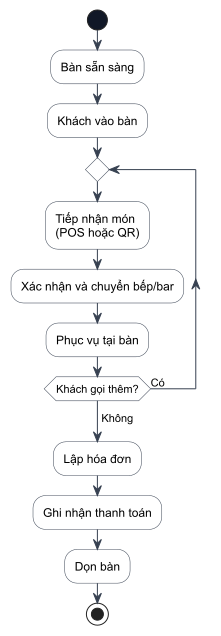
\includegraphics[width=\textwidth]{chapter2-fnb-pos-lifecycle.png}
  \caption{Vòng đời vận hành POS F\&B từ bàn đến thanh toán.}
  \label{fig:chapter2-fnb-pos-lifecycle}
\end{figure}

Bảng~\ref{tab:chapter2-pos-qr-comparison} tóm tắt sự khác biệt giữa POS truyền thống ở mức thu ngân và mô hình SaaS POS tích hợp đặt món qua QR mà khóa luận hướng đến. Bảng này không nhằm khẳng định một mô hình luôn tốt hơn mô hình kia trong mọi bối cảnh, mà chỉ làm rõ vì sao QRTable cần xử lý nhiều ràng buộc hơn một ứng dụng menu điện tử đơn giản.

{\footnotesize\sloppy
\setlength{\tabcolsep}{3pt}
\begin{longtable}{>{\raggedright\arraybackslash}p{0.21\textwidth}>{\raggedright\arraybackslash}p{0.32\textwidth}>{\raggedright\arraybackslash}p{0.36\textwidth}}
  \caption{So sánh POS truyền thống và SaaS POS tích hợp đặt món qua QR trong bối cảnh F\&B.}
  \label{tab:chapter2-pos-qr-comparison}\\
  \toprule
  Khía cạnh & POS truyền thống thiên về thu ngân & SaaS POS tích hợp đặt món qua QR \\
  \midrule
  \endfirsthead
  \toprule
  Khía cạnh & POS truyền thống thiên về thu ngân & SaaS POS tích hợp đặt món qua QR \\
  \midrule
  \endhead
  \bottomrule
  \endfoot
  Điểm bắt đầu nghiệp vụ & Nhân viên nhập đơn hoặc hóa đơn tại quầy/POS. & Khách có thể tự bắt đầu phiên gọi món bằng cách quét QR tại bàn. \\
  \addlinespace
  Phạm vi trạng thái & Thường tập trung vào đơn, hóa đơn và thanh toán. & Cần gắn đơn với tenant, bàn, phiên, giỏ chung, màn hình bếp (KDS), hóa đơn và vòng đời thanh toán. \\
  \addlinespace
  Vai trò người dùng & Chủ yếu là nhân viên, quản lý và chủ cửa hàng. & Có thêm khách ẩn danh theo phiên bàn và quản trị nền tảng (Super Admin) trong mô hình SaaS. \\
  \addlinespace
  Đồng bộ vận hành & Nhân viên là trung gian chính giữa khách và bếp. & Cần đồng bộ trực tiếp giữa ứng dụng khách (PWA), POS, KDS và thanh toán qua API và kênh thời gian thực. \\
  \addlinespace
  Triển khai & Có thể là phần mềm cài đặt riêng hoặc dịch vụ độc lập cho từng cửa hàng. & Nhiều nhà hàng dùng chung nền tảng, yêu cầu cô lập tenant, gói thuê bao và hạn mức sử dụng. \\
  \addlinespace
  Rủi ro kỹ thuật nổi bật & Sai sót nhập liệu, đồng bộ ca, lỗi tính tiền hoặc báo cáo. & QR giả/sai bàn, rò rỉ phiên, đơn trùng lặp, webhook trùng, rò rỉ dữ liệu giữa các tenant. \\
\end{longtable}
}

Từ góc nhìn nghiên cứu phần mềm, vấn đề không nằm ở việc số hóa menu bằng mã QR đơn lẻ, mà ở việc tích hợp đặt món qua QR vào một POS vận hành đầy đủ. Một mã QR chỉ là điểm vào; hệ thống phía sau mới quyết định việc nhận diện bàn, ràng buộc phiên, cập nhật giỏ hàng chung, xác nhận đơn, điều phối bếp và thanh toán có nhất quán hay không.

\section{Đặt món qua mã QR}

Mã QR là một dạng mã vạch hai chiều được chuẩn hóa. ISO/IEC 18004:2024 mô tả mã QR ở mức ký hiệu mã, bao gồm đặc tính mã, phương pháp mã hóa ký tự, định dạng biểu tượng, đặc tính kích thước, quy tắc sửa lỗi và các tham số ứng dụng \cite{iso-iec-18004-2024}. Trong bối cảnh F\&B, mã QR thường được dùng như một đường dẫn để khách truy cập thực đơn điện tử hoặc phiên gọi món của một bàn.

Một hệ thống đặt món qua QR đơn giản có thể chỉ cần hiển thị thực đơn sau khi khách quét mã. Tuy nhiên, đặt món qua QR trong POS nhà hàng có nhiều yêu cầu hơn. Mã QR phải xác định đúng tenant và bàn, token phải chống việc sửa URL tùy tiện, hệ thống phải biết khi nào tạo phiên mới hoặc cho khách tham gia phiên đang tồn tại, và các thao tác trên giỏ hàng phải được đồng bộ giữa nhiều thiết bị của cùng bàn. Nếu nhiều khách cùng quét một mã QR, họ không nên tạo ra nhiều phiên bàn độc lập gây trùng đơn hoặc chia sai hóa đơn.

Lợi ích thực tiễn của đặt món qua QR là giảm thao tác trung gian của nhân viên, giúp khách truy cập thực đơn nhanh hơn và hỗ trợ gọi thêm món trong lúc đang dùng bữa. Các nền tảng POS F\&B tại Việt Nam đã cung cấp hoặc mô tả các luồng gọi món qua QR trong tài liệu sản phẩm, ví dụ KiotViet hướng dẫn chức năng gọi món qua mã QR \cite{kiotviet-qr-order-doc}, còn iPOS mô tả giải pháp đặt món O2O/QR cho vận hành nhà hàng \cite{ipos-o2o-qr-order}. Những nguồn này cho thấy đặt món qua QR là nhu cầu sản phẩm thực tế, nhưng không phải bằng chứng học thuật rằng mọi hệ thống như vậy đều đúng, an toàn hoặc phù hợp với kiến trúc microservices.

Thách thức quan trọng là xác thực ngữ cảnh. Khác với nhân viên đăng nhập bằng tài khoản, khách hàng thường không muốn tạo tài khoản chỉ để gọi món tại bàn. Vì vậy, hệ thống phải cân bằng giữa trải nghiệm thuận tiện và kiểm soát bảo mật. Token QR, token phiên, giới hạn tần suất, trạng thái bàn và ngữ cảnh tenant trở thành các lớp kiểm soát thay cho mô hình đăng nhập truyền thống.

Thách thức thứ hai là chống trùng lặp. Mạng di động có thể chập chờn, khách có thể bấm gửi lại, trình duyệt có thể gửi lại yêu cầu, hoặc nhiều khách cùng bàn có thể thao tác gần như đồng thời. Nếu hệ thống không có khóa xử lý lặp an toàn (idempotency) hoặc phiên bản giỏ hàng, cùng một đơn có thể bị tạo nhiều lần hoặc giỏ hàng có thể bị ghi đè. Vì vậy, luồng đặt món qua QR không thể chỉ được thiết kế như một lần gửi biểu mẫu đơn giản.

Thách thức thứ ba là liên kết cập nhật thời gian thực với nguồn trạng thái đáng tin. Khách và nhân viên đều mong muốn thấy trạng thái đơn hoặc bếp cập nhật nhanh, nhưng kênh thời gian thực không nên trở thành nơi quyết định trạng thái nghiệp vụ cuối cùng. Thiết kế an toàn hơn là dùng thông báo thời gian thực để báo ứng dụng phía người dùng tải lại bản chụp trạng thái từ API của dịch vụ sở hữu dữ liệu. Nguyên tắc này sẽ được nối với WebSocket ở mục~\ref{sec:chapter2-realtime}.

Hình~\ref{fig:chapter2-qr-ordering-flow} minh họa luồng khái niệm từ quét QR đến gửi đơn, nhấn mạnh các lớp kiểm soát phiên và chống trùng lặp.

\begin{figure}[htbp]
  \centering
  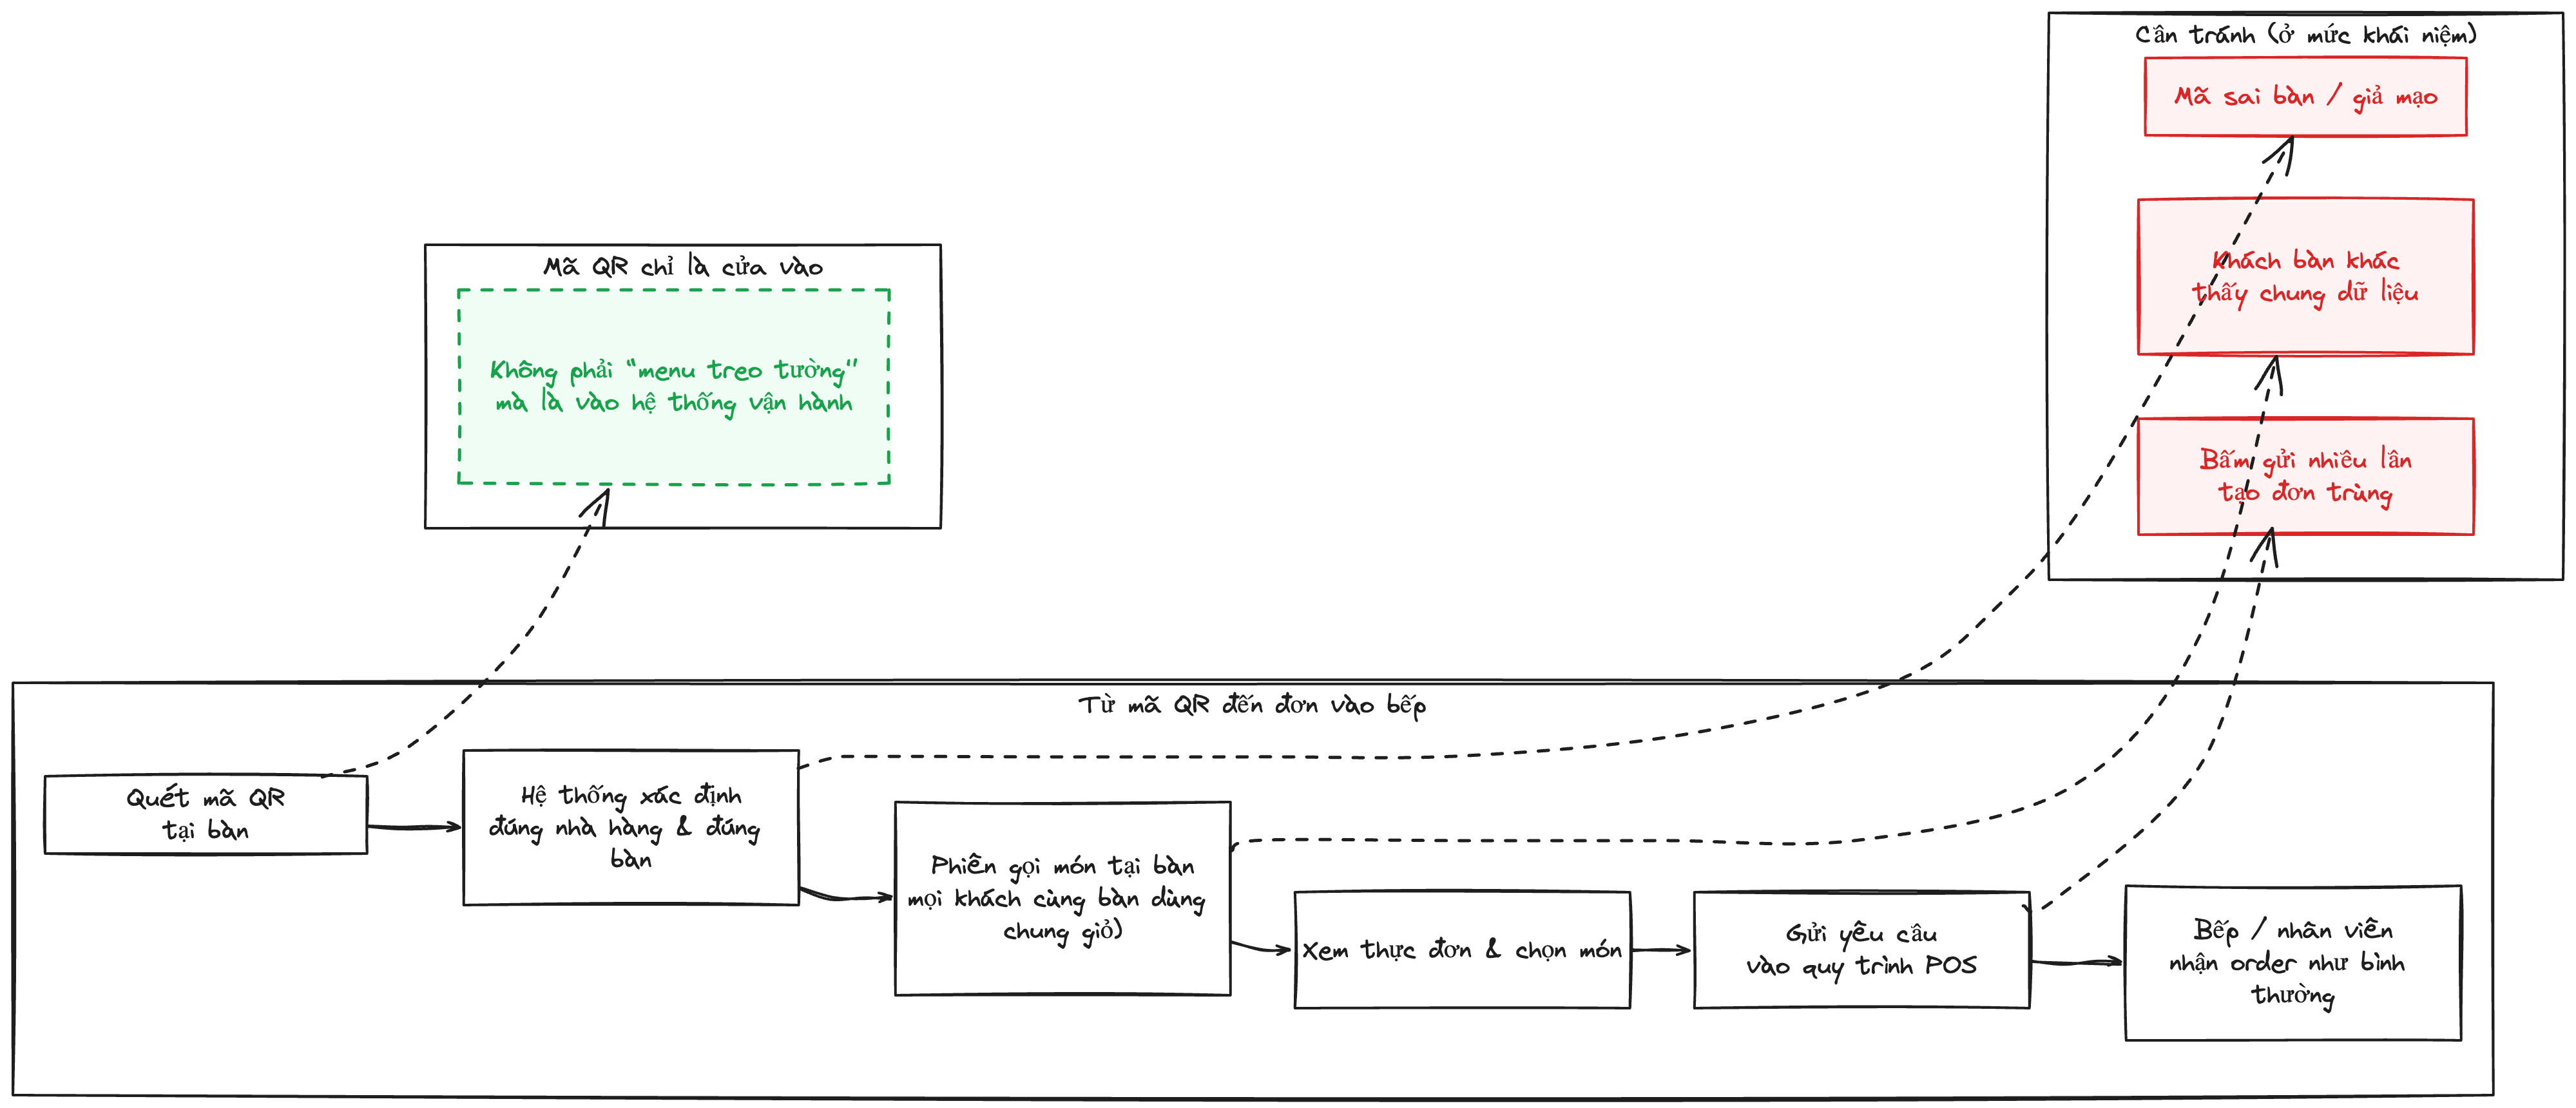
\includegraphics[width=\textwidth]{chapter2-qr-ordering-flow.png}
  \caption{Luồng đặt món qua mã QR ở mức khái niệm.}
  \label{fig:chapter2-qr-ordering-flow}
\end{figure}

\section{SaaS và mô hình đa tenant}

NIST định nghĩa điện toán đám mây là mô hình cho phép truy cập mạng thuận tiện, theo nhu cầu, tới một nhóm tài nguyên tính toán dùng chung có thể được cấp phát và thu hồi nhanh với ít công sức quản trị \cite{nist-sp800145-2011}. Trong các mô hình dịch vụ đám mây, SaaS cho phép người dùng sử dụng ứng dụng của nhà cung cấp chạy trên hạ tầng đám mây mà không quản trị trực tiếp hạ tầng, hệ điều hành hoặc phần lớn thành phần nền bên dưới. Đối với QRTable, ý nghĩa thực tiễn của SaaS là nhiều nhà hàng có thể sử dụng cùng một nền tảng POS thay vì mỗi nhà hàng tự triển khai một hệ thống riêng.

Đa tenant là vấn đề trung tâm của SaaS. Một tenant có thể hiểu là một đơn vị khách hàng hoặc tổ chức sử dụng hệ thống như một phạm vi vận hành riêng. Trong QRTable, một tenant tương ứng với một nhà hàng hoặc chuỗi nhà hàng trong phạm vi đề tài. Mỗi tenant có dữ liệu riêng về thực đơn, bàn, nhân sự, đơn hàng, cấu hình thanh toán, gói thuê bao và trạng thái vận hành. Dù nhiều tenant dùng chung mã nguồn và hạ tầng, dữ liệu và quyền truy cập của họ phải được cô lập.

Đa tenant không chỉ là một quyết định về cơ sở dữ liệu. Nó liên quan đến API, xác thực, phân quyền, bộ nhớ đệm, sự kiện, phòng thời gian thực, tải tệp và cả tham chiếu thanh toán. Nếu chỉ lọc tenant ở cơ sở dữ liệu nhưng khóa bộ nhớ đệm hoặc phòng WebSocket không gắn không gian tên tenant, hệ thống vẫn có nguy cơ lộ dữ liệu chéo tenant. Vì vậy, cô lập tenant phải được xem là ràng buộc bất biến xuyên suốt kiến trúc.

Microsoft Azure Architecture Center mô tả khi thiết kế lưu trữ dữ liệu cho hệ thống đa tenant cần quyết định mức chia sẻ hoặc cô lập dữ liệu giữa các tenant, đồng thời có thể chọn một mẫu nhất quán hoặc kết hợp nhiều mẫu tùy quy mô và yêu cầu \cite{microsoft-multitenant-storage-data-2026}. Hình~\ref{fig:chapter2-saas-multitenancy} minh họa mô hình nhiều tenant trên nền tảng dùng chung và ranh giới cô lập xuyên suốt. Bảng~\ref{tab:chapter2-multitenancy-models} tóm tắt một số mô hình phổ biến ở mức khái niệm.

\begin{figure}[htbp]
  \centering
  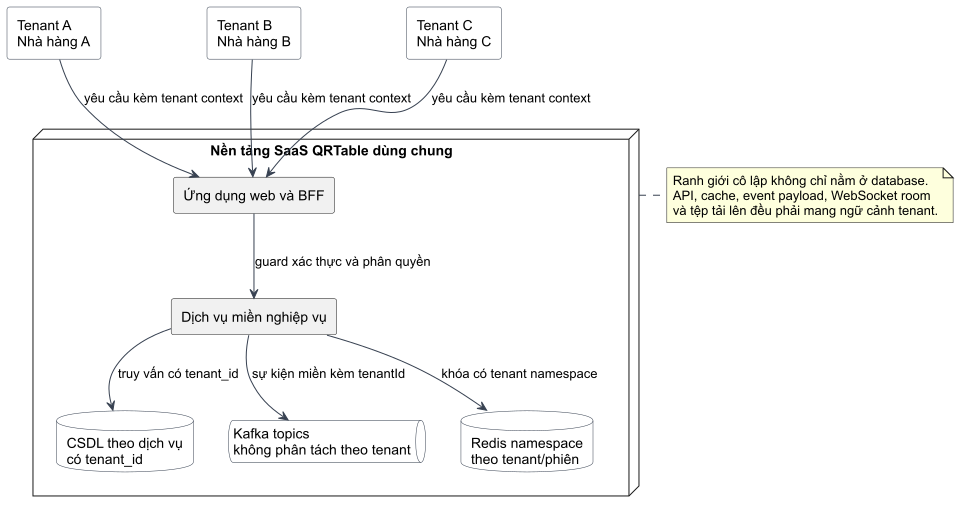
\includegraphics[width=\textwidth]{chapter2-saas-multitenancy.png}
  \caption{Mô hình khái niệm SaaS đa tenant và ranh giới cô lập.}
  \label{fig:chapter2-saas-multitenancy}
\end{figure}

{\footnotesize\sloppy
\setlength{\tabcolsep}{3pt}
\begin{longtable}{>{\raggedright\arraybackslash}p{0.2\textwidth}>{\raggedright\arraybackslash}p{0.25\textwidth}>{\raggedright\arraybackslash}p{0.22\textwidth}>{\raggedright\arraybackslash}p{0.23\textwidth}}
  \caption{So sánh các mô hình lưu trữ dữ liệu trong kiến trúc đa tenant.}
  \label{tab:chapter2-multitenancy-models}\\
  \toprule
  Mô hình & Đặc điểm & Ưu điểm & Hạn chế / rủi ro \\
  \midrule
  \endfirsthead
  \toprule
  Mô hình & Đặc điểm & Ưu điểm & Hạn chế / rủi ro \\
  \midrule
  \endhead
  \bottomrule
  \endfoot
  CSDL chung, lược đồ chung & Nhiều tenant dùng chung cơ sở dữ liệu/lược đồ; bảng có cột phân biệt tenant như \texttt{tenant\_id}. & Chi phí vận hành thấp, di chuyển lược đồ đơn giản, phù hợp giai đoạn đầu. & Cần bộ lọc truy vấn nghiêm ngặt; lỗi lọc tenant có thể gây rò rỉ dữ liệu. \\
  \addlinespace
  CSDL chung, lược đồ riêng mỗi tenant & Tenant dùng chung máy chủ CSDL nhưng có lược đồ riêng. & Cô lập tốt hơn ở lớp lược đồ, dễ sao lưu/di chuyển theo tenant hơn mô hình lược đồ chung. & Số lượng lược đồ lớn làm di chuyển và vận hành phức tạp. \\
  \addlinespace
  CSDL riêng mỗi tenant & Mỗi tenant có cơ sở dữ liệu riêng. & Cô lập vật lý cao hơn, dễ đáp ứng yêu cầu tuân thủ hoặc khách hàng lớn. & Chi phí và tự động hóa vận hành cao; khó tối ưu tài nguyên cho nhiều tenant nhỏ. \\
  \addlinespace
  Lai ghép / triển khai tách & Kết hợp nhiều mức cô lập, ví dụ tenant nhỏ dùng mô hình chung, tenant lớn dùng triển khai tách. & Linh hoạt theo gói dịch vụ, quy mô và yêu cầu đặc biệt của tenant. & Kiến trúc và tự động hóa phức tạp hơn; cần quản trị vòng đời rõ. \\
\end{longtable}
}

Trong một SaaS POS cho F\&B, việc chọn mô hình đa tenant phải cân bằng giữa chi phí, độ phức tạp và mức cô lập. Với hệ thống khóa luận hoặc giai đoạn sản phẩm ban đầu, lược đồ chung có \texttt{tenant\_id} kết hợp kiểm soát ở API, bộ nhớ đệm và sự kiện có thể là lựa chọn thực dụng. Với quy mô lớn hơn, tenant có yêu cầu tuân thủ cao hoặc dữ liệu nhạy cảm hơn, mô hình CSDL riêng mỗi tenant hoặc lai ghép có thể phù hợp hơn. Điều quan trọng là khóa luận không nên trình bày đa tenant như một lựa chọn duy nhất; mỗi mô hình đều có đánh đổi.

Ngoài cô lập dữ liệu, SaaS còn đặt ra bài toán vòng đời tenant. Tenant cần được tạo, cấu hình chủ sở hữu, gói dịch vụ, hạn mức, cấu hình thanh toán và trạng thái hoạt động. Khi tenant bị tạm ngưng, hệ thống phải xác định thao tác nào bị chặn, thao tác nào vẫn được xử lý để không làm mất trạng thái tiền hoặc đơn hàng đã phát sinh. Đây là điểm khác biệt giữa một ứng dụng POS đơn lẻ và nền tảng SaaS POS có quản trị tenant.

\section{Kiến trúc microservices}

Microservices là một phong cách kiến trúc trong đó hệ thống được tổ chức thành nhiều dịch vụ nhỏ, mỗi dịch vụ chạy trong tiến trình riêng, giao tiếp qua cơ chế nhẹ và có thể được triển khai độc lập theo năng lực nghiệp vụ. Lewis và Fowler nhấn mạnh các đặc trưng như dịch vụ theo năng lực nghiệp vụ, tự động hóa triển khai, quản lý dữ liệu phân tán và thiết kế chịu lỗi \cite{lewis-fowler-microservices-2014}. Trong ngữ cảnh QRTable, microservices được xem là cách tách các ngữ cảnh giới hạn như thực đơn (Catalog), đơn hàng (Order), bếp (Kitchen), thanh toán (Payment), SaaS và truy cập người dùng (User-Access).

Lợi ích chính của microservices không phải là hiệu năng tự động cao hơn. Lợi ích quan trọng hơn là làm rõ trách nhiệm sở hữu dữ liệu và giảm gắn kết theo miền nghiệp vụ. Dịch vụ thực đơn sở hữu menu, bàn và tồn kho; dịch vụ đơn hàng sở hữu phiên, giỏ, đơn và hóa đơn; dịch vụ thanh toán sở hữu quyết toán và cấu hình thanh toán; dịch vụ bếp sở hữu chiếu KDS; dịch vụ SaaS sở hữu vòng đời tenant và gói thuê bao. Khi trách nhiệm rõ, các ràng buộc nghiệp vụ có nơi đặt cụ thể, ví dụ chỉ dịch vụ thực đơn được quyết định tồn kho, chỉ dịch vụ đơn hàng được quyết định vòng đời đơn/hóa đơn, chỉ dịch vụ thanh toán được quyết định trạng thái giao dịch thanh toán.

Newman nhấn mạnh việc thiết kế ranh giới dịch vụ phải quan tâm đến gắn kết, độ gắn kết nội bộ và khả năng thay đổi độc lập \cite{newman-building-microservices-2021}. Nếu chia dịch vụ theo tầng kỹ thuật hoặc theo tên bảng thay vì miền nghiệp vụ, hệ thống vẫn gắn kết cao nhưng lại gánh thêm chi phí phân tán. Vì vậy, microservices cần đi cùng ranh giới dịch vụ có nghĩa nghiệp vụ, không chỉ là nhiều thư mục hoặc nhiều container.

Richardson mô tả các mẫu quan trọng trong microservices như cơ sở dữ liệu riêng mỗi dịch vụ, saga và nhắn tin giao dịch \cite{richardson-microservices-patterns-2018}. Mô hình cơ sở dữ liệu riêng giúp mỗi dịch vụ kiểm soát dữ liệu và lược đồ của mình, nhưng đổi lại các truy vấn hoặc giao dịch xuyên dịch vụ trở nên khó hơn. Hệ thống phải chọn giữa giao tiếp đồng bộ, sự kiện bất đồng bộ, mô hình đọc sao chép, saga hoặc outbox tùy tình huống. Đây là lý do microservices phù hợp với bài toán nhiều ngữ cảnh giới hạn nhưng cũng tạo độ phức tạp phân tán.

Các đánh đổi chính của microservices gồm:

\begin{itemize}
  \item \textbf{Độ phức tạp giao tiếp}: thay vì gọi hàm trong cùng tiến trình, dịch vụ phải xử lý lỗi mạng, hết thời gian chờ, gửi lại và tuần tự hóa dữ liệu.
  \item \textbf{Nhất quán dữ liệu}: giao dịch ACID trong một cơ sở dữ liệu không còn bao phủ toàn bộ luồng xuyên dịch vụ.
  \item \textbf{Quan sát lỗi phân tán}: lỗi có thể nằm ở bên phát, bên tiêu thụ, trình môi giới, bộ nhớ đệm, cổng hoặc dịch vụ hạ nguồn.
  \item \textbf{Chi phí vận hành}: nhiều dịch vụ cần cấu hình, triển khai, ghi nhật ký, kiểm tra sức khỏe, quản lý phiên bản và hợp đồng giao tiếp.
\end{itemize}

Do đó, một khóa luận không nên dùng microservices như một khẩu hiệu. Quyết định dùng microservices chỉ thuyết phục khi có các miền nghiệp vụ thực sự khác nhau, có trách nhiệm dữ liệu riêng và có lý do bảo trì, mở rộng rõ. Với QRTable, cơ sở lập luận là hệ thống có nhiều miền vận hành tương đối độc lập: vòng đời tenant, thực đơn/bàn/QR, đơn/phiên/hóa đơn, hàng đợi bếp, quyết toán thanh toán và truy cập người dùng.

Hình~\ref{fig:chapter2-monolith-vs-microservices} so sánh kiến trúc monolith và microservices theo ngữ cảnh giới hạn và mô hình cơ sở dữ liệu riêng. Bảng~\ref{tab:chapter2-architecture-styles} tóm tắt đánh đổi ở mức khái niệm.

\begin{figure}[htbp]
  \centering
  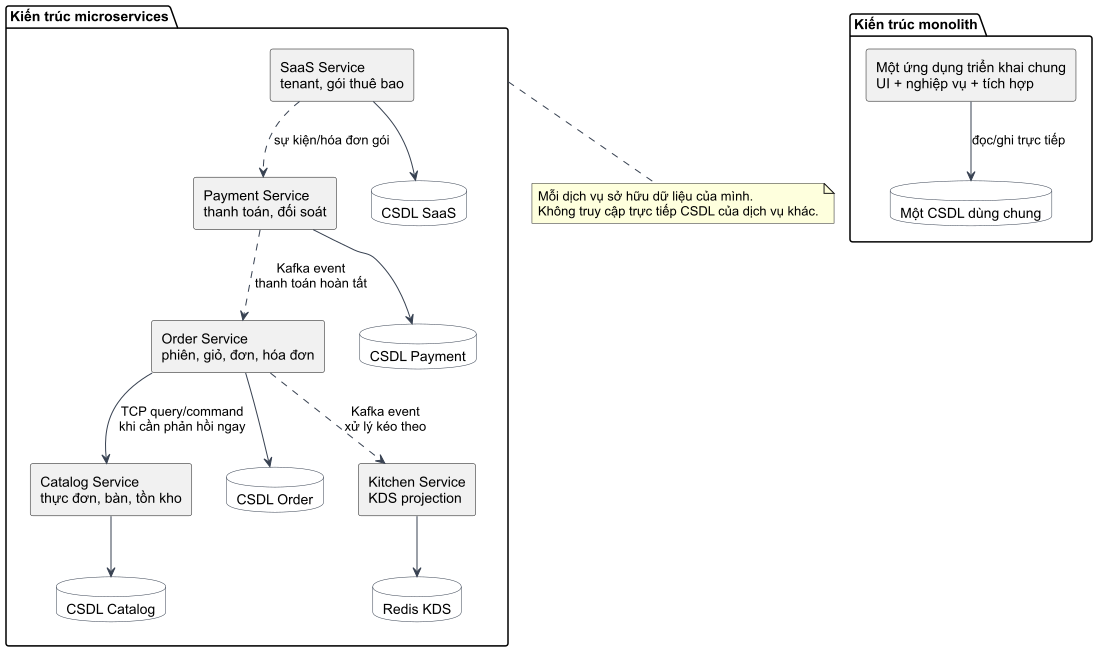
\includegraphics[width=\textwidth]{chapter2-monolith-vs-microservices.png}
  \caption{So sánh monolith và microservices theo ngữ cảnh giới hạn nghiệp vụ.}
  \label{fig:chapter2-monolith-vs-microservices}
\end{figure}

{\footnotesize\sloppy
\setlength{\tabcolsep}{3pt}
\begin{longtable}{>{\raggedright\arraybackslash}p{0.22\textwidth}>{\raggedright\arraybackslash}p{0.3\textwidth}>{\raggedright\arraybackslash}p{0.2\textwidth}>{\raggedright\arraybackslash}p{0.2\textwidth}}
  \caption{So sánh monolith, modular monolith và microservices.}
  \label{tab:chapter2-architecture-styles}\\
  \toprule
  Kiểu kiến trúc & Đặc điểm & Ưu điểm & Hạn chế \\
  \midrule
  \endfirsthead
  \toprule
  Kiểu kiến trúc & Đặc điểm & Ưu điểm & Hạn chế \\
  \midrule
  \endhead
  \bottomrule
  \endfoot
  Monolith & Một ứng dụng, thường một cơ sở dữ liệu. & Triển khai và gỡ lỗi đơn giản; giao dịch ACID nội bộ. & Gắn kết tăng theo thời gian; khó mở rộng theo miền nghiệp vụ. \\
  \addlinespace
  Monolith mô-đun & Một gói triển khai nhưng module/miền tách trong mã nguồn. & Cân bằng đơn giản vận hành và ranh giới miền. & Vẫn chia sẻ runtime và CSDL nếu không kiểm soát ranh giới. \\
  \addlinespace
  Microservices & Nhiều dịch vụ độc lập, CSDL riêng mỗi dịch vụ. & Mở rộng và thay đổi theo miền; trách nhiệm sở hữu rõ. & Độ phức tạp phân tán, nhất quán và quan sát khó hơn. \\
\end{longtable}
}

\section{Kiến trúc hướng sự kiện và Apache Kafka}

Kiến trúc hướng sự kiện tổ chức hệ thống quanh các sự kiện biểu diễn việc đã xảy ra trong miền nghiệp vụ, ví dụ đơn đã được xác nhận hoặc thanh toán đã hoàn tất. Thay vì dịch vụ A gọi trực tiếp dịch vụ B để thực hiện mọi xử lý kéo theo, dịch vụ A có thể phát hành sự kiện và các bên tiêu thụ liên quan xử lý bất đồng bộ. Cách tiếp cận này tách rời theo thời gian: bên phát không cần biết bên tiêu thụ đang chạy ngay lúc đó hoặc có bao nhiêu bên cùng quan tâm tới sự kiện.

Apache Kafka là một nền tảng truyền phát sự kiện phân tán. Tài liệu chính thức của Kafka trình bày các khái niệm như bản ghi sự kiện, topic, producer, consumer, phân vùng (partition) và nhóm consumer \cite{apache-kafka-docs-2026}. Producer ghi sự kiện vào topic; consumer đọc sự kiện từ topic; phân vùng giúp chia dữ liệu và xử lý song song; nhóm consumer giúp nhiều phiên bản cùng xử lý một tập sự kiện theo cách phối hợp.

Hình~\ref{fig:chapter2-kafka-event-flow} minh họa luồng hướng sự kiện với topic, phân vùng và nhóm consumer.

\begin{figure}[htbp]
  \centering
  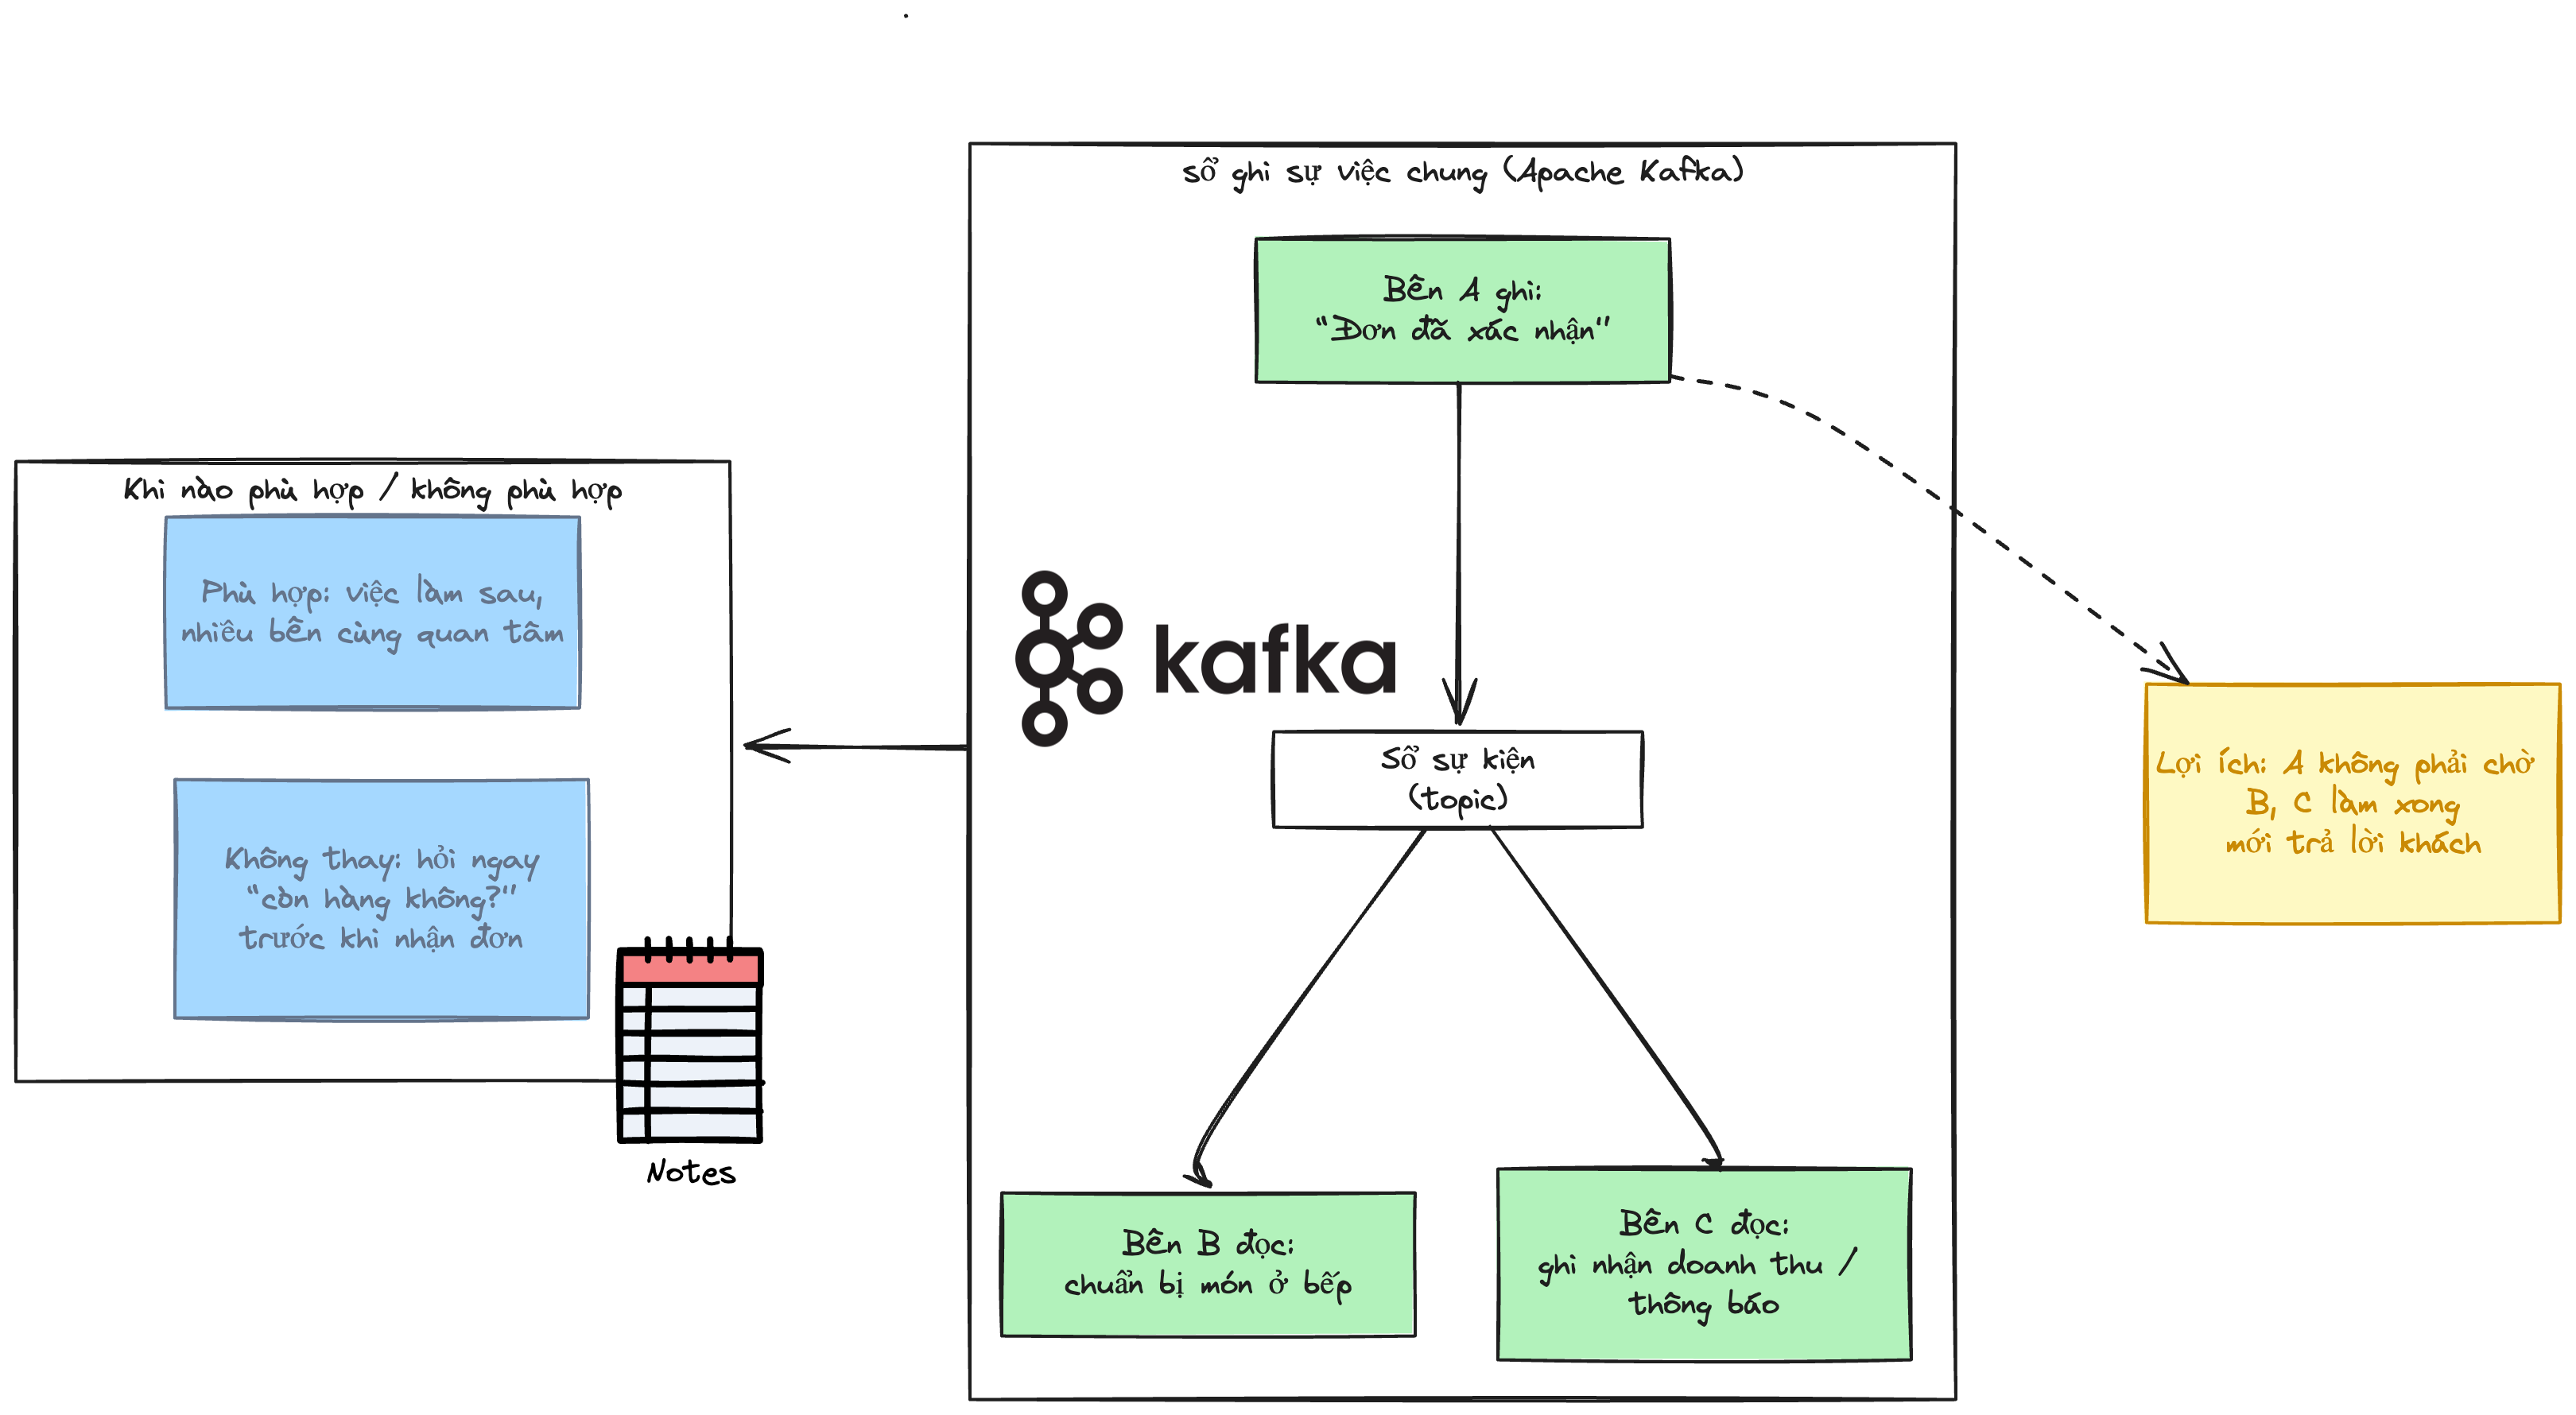
\includegraphics[width=\textwidth]{chapter2-kafka-event-flow.png}
  \caption{Luồng hướng sự kiện với topic, phân vùng và nhóm consumer.}
  \label{fig:chapter2-kafka-event-flow}
\end{figure}

Kafka phù hợp với các tình huống cần lưu và truyền sự kiện bền vững, phát tán tới nhiều bên tiêu thụ (consumer), xử lý bất đồng bộ hoặc khôi phục bên tiêu thụ sau sự cố. Trong QRTable, ví dụ điển hình là khi đơn đã được xác nhận, dịch vụ bếp có thể tạo phiếu KDS từ sự kiện \texttt{order.confirmed}; hoặc khi thanh toán hoàn tất, hệ thống có thể phát sự kiện để các thành phần liên quan cập nhật trạng thái hoặc gửi gợi ý thời gian thực. Bên phát không nhất thiết phải chờ mọi xử lý kéo theo hoàn thành trước khi trả lời người dùng.

Tuy nhiên, Kafka không nên được dùng thay cho mọi lời gọi đồng bộ. Nếu một lệnh cần biết kết quả ngay để quyết định giao dịch, ví dụ dịch vụ đơn hàng cần biết dịch vụ thực đơn có trừ tồn kho thành công hay không trước khi chuyển đơn sang trạng thái xử lý, gọi RPC đồng bộ thường phù hợp hơn. Nếu thao tác chỉ là thông báo giao diện sau khi lớp BFF đã có phản hồi, WebSocket hoặc kênh trực tiếp qua BFF có thể đơn giản hơn Kafka. Nếu dùng Kafka cho mọi việc, hệ thống có thể tăng độ trễ, khó gỡ lỗi và làm mờ ranh giới giao dịch.

Bảng~\ref{tab:chapter2-sync-async-communication} so sánh giao tiếp đồng bộ và bất đồng bộ trong microservices. Bảng này là nền cho khung quyết định ở Chương 4, nơi QRTable chọn TCP/gRPC cho lệnh/truy vấn cần phản hồi và Kafka cho sự kiện miền nghiệp vụ và xử lý kéo theo bất đồng bộ.

{\footnotesize\sloppy
\setlength{\tabcolsep}{3pt}
\begin{longtable}{>{\raggedright\arraybackslash}p{0.18\textwidth}>{\raggedright\arraybackslash}p{0.32\textwidth}>{\raggedright\arraybackslash}p{0.34\textwidth}}
  \caption{So sánh giao tiếp đồng bộ và bất đồng bộ trong microservices.}
  \label{tab:chapter2-sync-async-communication}\\
  \toprule
  Khía cạnh & Giao tiếp đồng bộ & Giao tiếp bất đồng bộ / hướng sự kiện \\
  \midrule
  \endfirsthead
  \toprule
  Khía cạnh & Giao tiếp đồng bộ & Giao tiếp bất đồng bộ / hướng sự kiện \\
  \midrule
  \endhead
  \bottomrule
  \endfoot
  Mục tiêu chính & Lấy kết quả ngay cho lệnh/truy vấn. & Phát sinh sự kiện để bên tiêu thụ xử lý sau hoặc song song. \\
  \addlinespace
  Gắn kết thời gian & Bên gọi và bên được gọi cần sẵn sàng cùng thời điểm. & Bên phát và bên tiêu thụ tách nhau hơn về thời gian. \\
  \addlinespace
  Ví dụ phù hợp & Xác thực QR, lấy thực đơn, trừ tồn kho khi xác nhận đơn, lấy bản chụp hóa đơn. & Tạo phiếu KDS sau khi đơn xác nhận, phát tán khi thanh toán xong, cảnh báo SLA. \\
  \addlinespace
  Ưu điểm & Dễ hiểu, dễ trả lỗi tức thời, phù hợp ranh giới giao dịch cần quyết định ngay. & Tách rời tốt hơn, mở rộng bên tiêu thụ, hỗ trợ phát lại/khôi phục tùy cấu hình broker. \\
  \addlinespace
  Hạn chế & Dễ lan truyền lỗi/hết thời gian chờ, gắn kết runtime cao hơn. & Khó gỡ lỗi hơn, cần consumer xử lý lặp an toàn, nhất quán dần và giám sát tốt. \\
  \addlinespace
  Nguyên tắc trong QRTable & Không dùng để phát tán xử lý kéo theo không cần chờ. & Không dùng thay mọi RPC hoặc làm nguồn trạng thái cuối của giao diện. \\
\end{longtable}
}

Một điểm cần nhấn mạnh là sự kiện không thay thế giao dịch cơ sở dữ liệu. Kafka có thể giúp truyền đạt rằng một việc đã xảy ra, nhưng tính đúng đắn của nghiệp vụ vẫn phụ thuộc vào ranh giới giao dịch và dịch vụ sở hữu dữ liệu. Nếu dịch vụ đơn hàng phát sự kiện trước khi giao dịch CSDL hoàn tất, hoặc giao dịch CSDL thành công nhưng phát sự kiện thất bại, hệ thống có nguy cơ ghi kép (dual-write). Vì vậy, các mẫu như outbox giao dịch thường được dùng để giảm rủi ro giữa ghi CSDL và phát hành sự kiện \cite{richardson-microservices-patterns-2018}. Chương 4 và Chương 5 sẽ chỉ khẳng định mức QRTable đã triển khai khi có bằng chứng mã nguồn hoặc kiểm thử tương ứng.

\section{Nhất quán dữ liệu, xử lý lặp an toàn và các mẫu giao dịch phân tán}

Trong kiến trúc monolith dùng một cơ sở dữ liệu duy nhất, nhiều thao tác có thể được bao phủ bởi một giao dịch ACID. Trong microservices, mỗi dịch vụ sở hữu cơ sở dữ liệu riêng nên giao dịch xuyên dịch vụ không còn đơn giản. Ví dụ, xác nhận đơn trong QRTable liên quan đến CSDL đơn hàng, tồn kho thực đơn, sự kiện Kafka và chiếu bếp. Nếu cố gắng gom tất cả vào một giao dịch phân tán, hệ thống sẽ phức tạp và phụ thuộc hạ tầng hơn; nếu tách rời hoàn toàn, hệ thống phải chấp nhận nhất quán dần và thiết kế bù trừ phù hợp.

Nhất quán dữ liệu trong microservices vì vậy cần được hiểu theo từng ràng buộc nghiệp vụ. Ràng buộc tồn kho thuộc dịch vụ thực đơn; ràng buộc vòng đời đơn thuộc dịch vụ đơn hàng; ràng buộc quyết toán thanh toán thuộc dịch vụ thanh toán; ràng buộc vòng đời tenant thuộc dịch vụ SaaS. Mỗi dịch vụ nên đảm bảo tính nhất quán mạnh trong phạm vi dữ liệu mình sở hữu. Khi cần phối hợp với dịch vụ khác, hệ thống dùng RPC, sự kiện, outbox, saga hoặc bù trừ tùy tính chất thao tác.

Xử lý lặp an toàn (idempotency) là khả năng xử lý một yêu cầu lặp lại mà không tạo thêm tác dụng phụ ngoài lần xử lý đầu tiên. Trong đặt món qua QR, cơ chế này cần cho việc gửi đơn vì khách hoặc trình duyệt có thể gửi yêu cầu lặp. Trong thanh toán, cần cho webhook vì nhà cung cấp có thể gửi lại cùng một thông báo. Trong luồng hướng sự kiện, cần cho consumer vì cùng một sự kiện có thể được xử lý lại khi gửi lại hoặc cân bằng lại nhóm.

Saga là một mẫu cổ điển cho giao dịch kéo dài. Garcia-Molina và Salem giới thiệu saga như một chuỗi giao dịch con, trong đó mỗi bước có thể có giao dịch bù trừ nếu cần hoàn tác logic nghiệp vụ \cite{garcia-molina-sagas-1987}. Trong microservices hiện đại, saga thường được diễn đạt như điều phối tập trung hoặc phối hợp phân tán giữa nhiều dịch vụ. Tuy nhiên, saga không phải cách làm cho mọi thao tác; nó phù hợp quy trình dài, nhiều bước, có bù trừ rõ và chấp nhận trạng thái trung gian.

Outbox là mẫu thường đi cùng hệ thống hướng sự kiện. Ý tưởng cơ bản là ghi thay đổi nghiệp vụ và thông điệp cần gửi vào cùng giao dịch CSDL của dịch vụ sở hữu; sau đó một tiến trình nền đưa thông điệp từ outbox ra trình môi giới. Mẫu này giảm rủi ro giữa hoàn tất giao dịch CSDL và phát hành sự kiện, nhưng vẫn cần xử lý gửi trùng, consumer idempotent và giám sát hàng đợi outbox.

Đối với QRTable, các khái niệm này tạo nền cho ba nguyên tắc:

\begin{itemize}
  \item Không dùng Kafka để thay thế giao dịch nghiệp vụ nội bộ của dịch vụ sở hữu dữ liệu.
  \item Không viết webhook hoặc consumer sự kiện như thao tác chỉ chạy đúng một lần.
  \item Không khẳng định saga/outbox đạt mức vận hành thực tế nếu mới có thiết kế cơ bản mà chưa kiểm chứng đầy đủ.
\end{itemize}

Hình~\ref{fig:chapter2-outbox-saga-overview} tóm tắt outbox giao dịch và saga phối hợp phân tán ở mức khái niệm.

\begin{figure}[htbp]
  \centering
  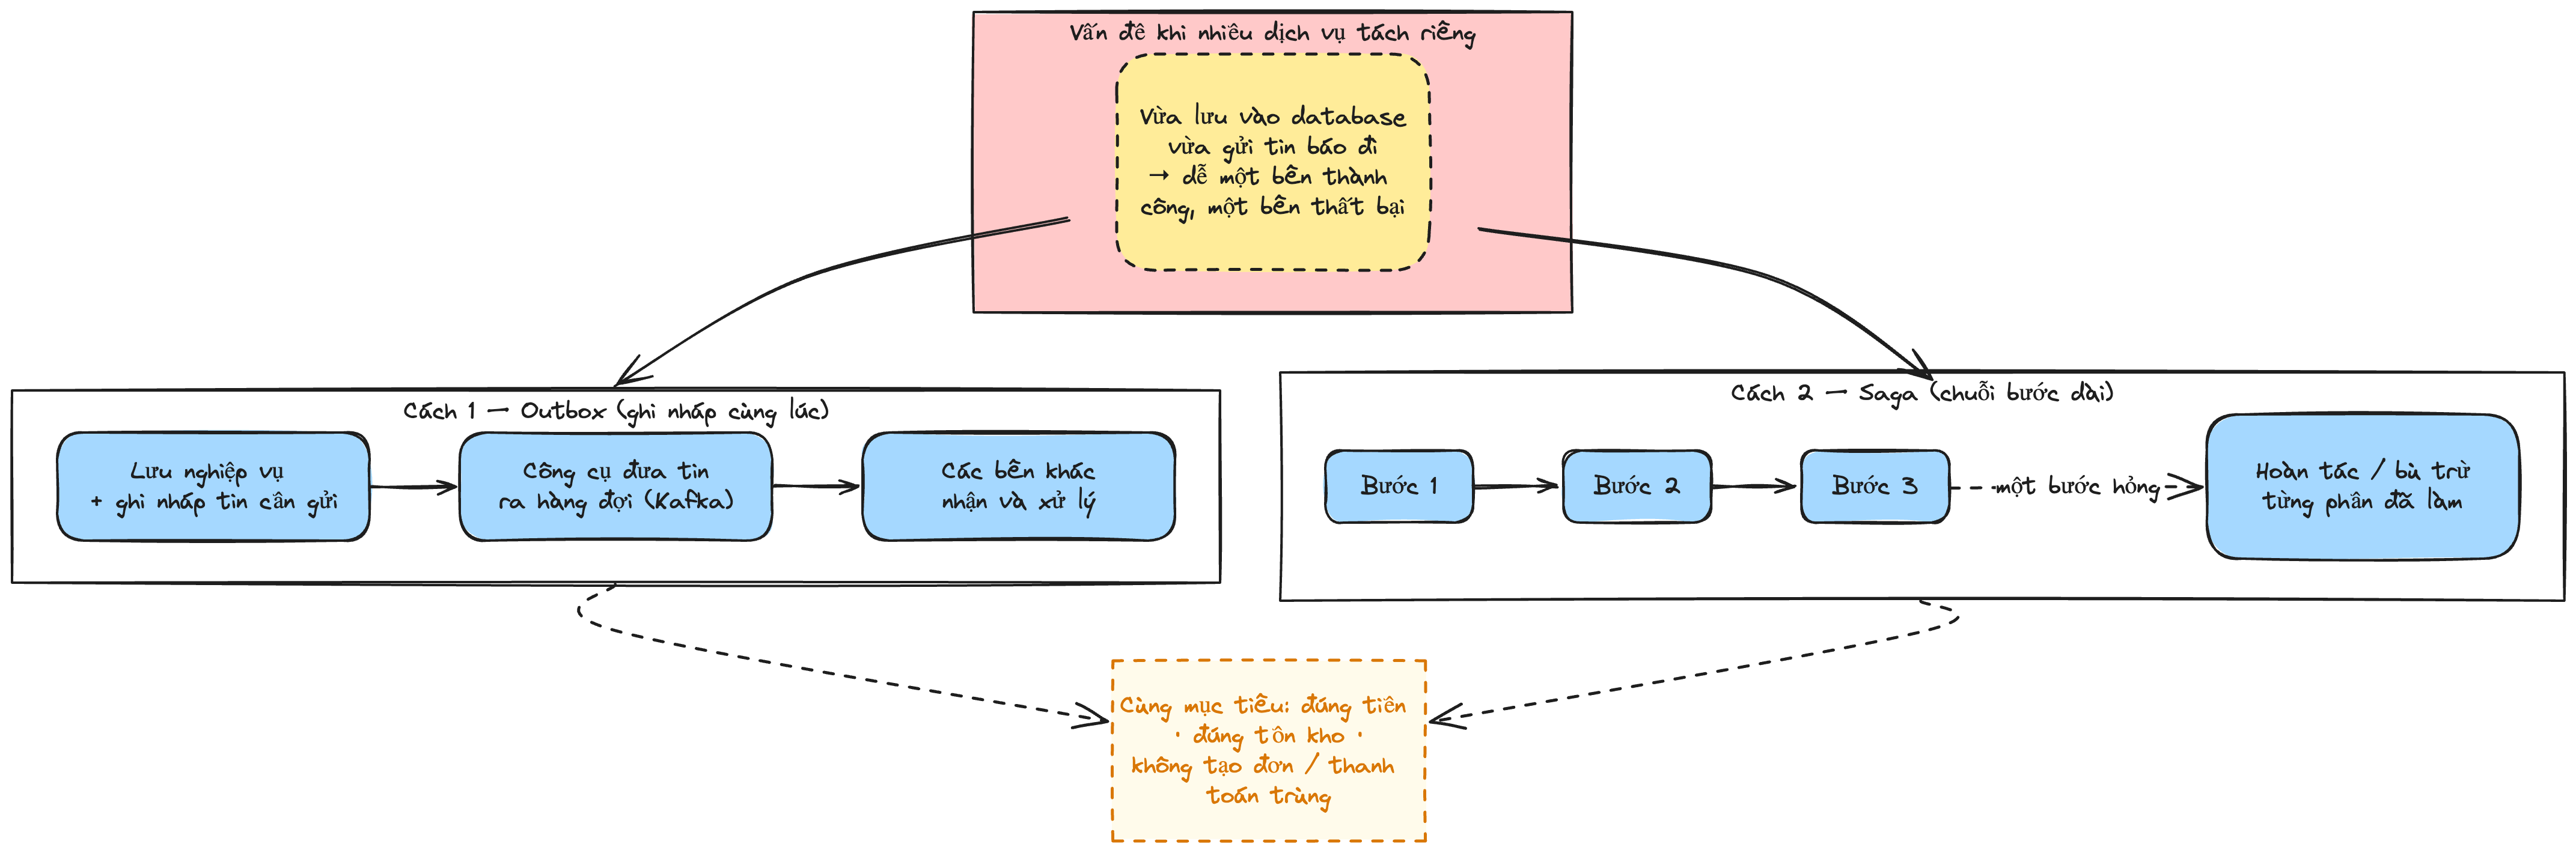
\includegraphics[width=\textwidth]{chapter2-outbox-saga-overview.png}
  \caption{Outbox giao dịch và saga phối hợp phân tán ở mức khái niệm.}
  \label{fig:chapter2-outbox-saga-overview}
\end{figure}

Những nguyên tắc này đặc biệt quan trọng trong thanh toán và tồn kho. Thanh toán sai có thể ảnh hưởng đến tiền; tồn kho sai có thể làm nhà hàng bán món đã hết hoặc từ chối món còn hàng; đơn trùng có thể làm bếp xử lý trùng. Vì vậy, các cơ chế nhất quán và xử lý lặp an toàn không phải tối ưu phụ, mà là yêu cầu đúng đắn nghiệp vụ.

\section{Giao tiếp thời gian thực}
\label{sec:chapter2-realtime}

Hình~\ref{fig:chapter2-websocket-hint-refetch} minh họa mô hình WebSocket như kênh gợi ý/thông báo và REST như nguồn trạng thái đáng tin.

\begin{figure}[htbp]
  \centering
  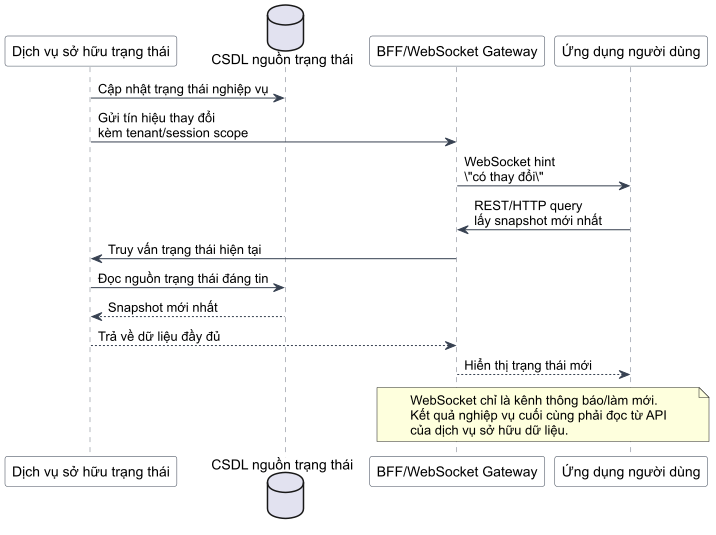
\includegraphics[width=\textwidth]{chapter2-websocket-hint-refetch.png}
  \caption{WebSocket gợi ý làm mới và nguồn trạng thái đáng tin.}
  \label{fig:chapter2-websocket-hint-refetch}
\end{figure}

WebSocket là giao thức cho phép giao tiếp hai chiều giữa ứng dụng phía client và máy chủ qua một kết nối TCP. RFC 6455 mô tả WebSocket như giải pháp thay thế việc hỏi lặp HTTP cho các ứng dụng web cần giao tiếp hai chiều, thời gian thực hơn giữa trang web và máy chủ \cite{fette-websocket-rfc6455-2011}. Trong POS F\&B, giao tiếp thời gian thực thường được dùng để cập nhật đơn mới cho nhân viên, phiếu mới cho bếp, trạng thái món cho khách hoặc cảnh báo thanh toán.

Lợi ích của cập nhật thời gian thực là giảm độ trễ nhận biết trên giao diện. Nếu khách gửi đơn, POS có thể nhận thông báo ngay để nhân viên xác nhận. Nếu đơn được xác nhận, KDS có thể nhận gợi ý để tải lại hàng đợi. Nếu thanh toán hoàn tất, giao diện POS hoặc khách có thể biết cần cập nhật hóa đơn và trạng thái bàn. Với trải nghiệm vận hành nhà hàng, các cập nhật này giúp giảm việc nhân viên phải làm mới trang thủ công.

Tuy nhiên, giao tiếp thời gian thực không đồng nghĩa với nguồn trạng thái đáng tin. Kết nối WebSocket có thể bị mất, ứng dụng có thể ngoại tuyến, sự kiện có thể đến trễ, hoặc người dùng có thể mở lại trình duyệt sau một khoảng thời gian. Nếu giao diện tin tuyệt đối vào nội dung sự kiện mà không tải lại trạng thái từ phía backend, trạng thái hiển thị có thể lệch với cơ sở dữ liệu hoặc dịch vụ sở hữu. Vì vậy, mẫu an toàn là dùng WebSocket như thông báo hoặc gợi ý làm mới: ứng dụng nhận tín hiệu, sau đó tải bản chụp trạng thái từ API.

Trong SaaS đa tenant, kênh thời gian thực còn cần kiểm soát phòng hoặc không gian tên. Nhân viên của tenant A không được nhận sự kiện của tenant B; khách của bàn này không được nhận sự kiện của bàn khác. Do đó, WebSocket phải gắn với ngữ cảnh tenant, phiên và bàn, kèm chuỗi kiểm soát truy cập tương ứng. Đây là lý do thiết kế thời gian thực không thể tách khỏi cô lập tenant và phân quyền.

Một điểm khác là thời gian thực không thay thế hàng đợi hoặc trình môi giới. WebSocket phù hợp để đẩy thông báo tới ứng dụng đang kết nối. Kafka phù hợp hơn cho sự kiện miền nghiệp vụ bền vững giữa các dịch vụ backend. Redis có thể phù hợp cho hàng đợi runtime hoặc pub/sub nội bộ. Việc chọn sai công cụ có thể làm hệ thống khó vận hành: dùng WebSocket để lưu sự kiện bền vững sẽ mất dữ liệu khi ứng dụng ngoại tuyến; dùng Kafka chỉ để báo giao diện làm mới sau một phản hồi HTTP có thể làm hệ thống nặng hơn cần thiết.

\section{Xác thực, phân quyền và bảo mật trong SaaS POS}

Xác thực trả lời câu hỏi người gọi là ai; phân quyền trả lời người đó có được phép thực hiện hành động hay không. Trong SaaS POS, hai câu hỏi này phải luôn đi cùng ngữ cảnh tenant. Chủ quán có quyền trong tenant của mình không có nghĩa người đó có quyền xem dữ liệu của tenant khác. Nhân viên có quyền xác nhận đơn không nhất thiết có quyền cập nhật cấu hình thanh toán hoặc gói thuê bao.

Hình~\ref{fig:chapter2-oidc-rbac-saas-pos} phân tách luồng xác thực nhân viên (OIDC/JWT/RBAC) và khách hàng theo phiên QR.

\begin{figure}[htbp]
  \centering
  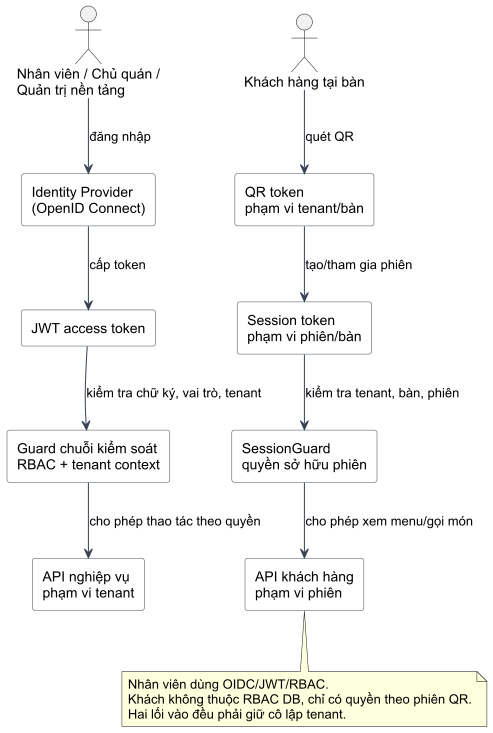
\includegraphics[width=\textwidth]{chapter2-oidc-rbac-saas-pos.png}
  \caption{Phân tách xác thực nhân viên (OIDC/JWT/RBAC) và khách theo phiên QR.}
  \label{fig:chapter2-oidc-rbac-saas-pos}
\end{figure}

JWT là định dạng token dùng để truyền các khẳng định (claims) dưới dạng JSON và có thể được ký hoặc bảo vệ toàn vẹn theo các cơ chế JOSE. RFC 7519 định nghĩa JWT như cách biểu diễn khẳng định gọn cho môi trường hạn chế kích thước như tiêu đề HTTP Authorization hoặc tham số truy vấn URI \cite{jones-jwt-rfc7519-2015}. Trong các hệ thống web hiện đại, JWT thường được dùng như token truy cập hoặc token danh tính, nhưng token chỉ an toàn khi được kiểm tra nhà phát hành, đối tượng, thời hạn, chữ ký và các khẳng định cần thiết theo ngữ cảnh ứng dụng.

OpenID Connect là lớp danh tính xây trên OAuth 2.0, cho phép ứng dụng client xác minh danh tính người dùng cuối dựa trên quá trình xác thực do máy chủ ủy quyền thực hiện, đồng thời nhận thông tin hồ sơ cơ bản theo cách tương tác chuẩn \cite{openid-connect-core-2023}. Với QRTable, nhóm nhân viên, chủ quán và quản trị có thể dùng Keycloak kết hợp OIDC/JWT để đăng nhập và gọi các API được bảo vệ. Tuy nhiên, khách quét QR tại bàn không nhất thiết là tài khoản trong hệ thống quản lý danh tính; khách nên được mô hình hóa như tác nhân theo phiên.

Phân quyền trong POS thường dùng RBAC (\textit{kiểm soát truy cập theo vai trò}) vì vai trò vận hành khá rõ: quản trị nền tảng, chủ quán, quản lý, phục vụ, bếp/bar. RBAC giúp gắn quyền với vai trò thay vì kiểm tra rời rạc ở từng màn hình. Tuy nhiên, điều hướng giao diện chỉ là lớp hỗ trợ trải nghiệm. Thực thi phân quyền phải nằm ở backend vì phía client có thể bị bỏ qua.

OWASP ASVS cung cấp chuẩn tham chiếu để kiểm tra các yêu cầu bảo mật ứng dụng, bao gồm xác thực, quản lý phiên, kiểm soát truy cập, kiểm tra đầu vào và nhiều nhóm kiểm soát khác \cite{owasp-asvs-2026}. Trong khóa luận này, ASVS được dùng như nguồn nền để diễn đạt các nhóm rủi ro và nguyên tắc kiểm soát, không phải để khẳng định QRTable đã đạt một mức ASVS cụ thể nếu chưa có đánh giá tương ứng.

Bảo mật trong SaaS POS còn bao gồm các rủi ro riêng:

\begin{itemize}
  \item \textbf{Truy cập chéo tenant}: người dùng hoặc yêu cầu của tenant này truy cập dữ liệu tenant khác.
  \item \textbf{Lạm dụng QR/phiên}: QR bị sửa, quét tràn, token phiên dùng sai bàn hoặc sai tenant.
  \item \textbf{Lạm dụng webhook thanh toán}: webhook giả, webhook trùng, thanh toán thiếu hoặc tham chiếu không khớp.
  \item \textbf{Lộ bí mật}: token, khóa webhook, trạng thái OAuth hoặc cấu hình thanh toán bị lộ ra giao diện hoặc nhật ký.
  \item \textbf{Leo thang đặc quyền}: vai trò nhân viên được cấp nhầm quyền chủ quán hoặc quản trị nền tảng.
\end{itemize}

ISO/IEC 25010:2023 đặt bảo mật là một thuộc tính chất lượng trong mô hình chất lượng sản phẩm, cùng với độ tin cậy, khả năng bảo trì và hiệu năng \cite{iso-iec-25010-2023}. Điều này giúp Chương 3 và Chương 6 diễn đạt bảo mật không chỉ như tính năng đăng nhập, mà là yêu cầu chất lượng xuyên suốt thiết kế và đánh giá.

\section{Các hệ thống và công trình liên quan}

Phần này xem xét các hệ thống, sản phẩm và nguồn liên quan ở mức phù hợp với phạm vi khóa luận. Vì QRTable là đề tài xây dựng hệ thống phần mềm ứng dụng, công trình liên quan không chỉ gồm bài báo học thuật mà còn gồm các nền tảng POS và đặt món qua QR thực tế trên thị trường Việt Nam. Tuy nhiên, cần phân biệt rõ: nguồn sản phẩm chỉ cho thấy chức năng tồn tại trên thị trường hoặc cách nhà cung cấp mô tả giải pháp; chúng không chứng minh khẳng định học thuật về kiến trúc, hiệu năng, bảo mật hoặc độ tin cậy.

KiotViet có tài liệu hướng dẫn gọi món qua mã QR trong ngữ cảnh F\&B \cite{kiotviet-qr-order-doc}. Nguồn này cho thấy một hướng triển khai phổ biến: khách quét QR để xem thực đơn và gọi món, còn nhà hàng quản lý đơn trong hệ thống POS. Sapo mô tả phần mềm quản lý nhà hàng, quán ăn với các chức năng vận hành như quản lý đơn, bàn, thanh toán và báo cáo \cite{sapo-fnb-restaurant-pos}. iPOS mô tả giải pháp đặt món O2O/QR nhằm tối ưu thao tác gọi món trong nhà hàng \cite{ipos-o2o-qr-order}. Các hệ thống này cho thấy đặt món qua QR và SaaS POS F\&B là nhu cầu thực tế, đặc biệt khi nhà hàng muốn giảm thao tác thủ công và tăng tốc phục vụ.

Bảng~\ref{tab:chapter2-related-systems} tóm tắt cách nhìn an toàn về các hệ thống liên quan. Bảng không so sánh hơn/thua vì khóa luận không có benchmark hoặc audit nội bộ của các sản phẩm thương mại. Thay vào đó, bảng xác định các khía cạnh liên quan đến QRTable và khoảng trống mà đề tài tập trung mô tả.

{\footnotesize\sloppy
\setlength{\tabcolsep}{3pt}
\begin{longtable}{>{\raggedright\arraybackslash}p{0.16\textwidth}>{\raggedright\arraybackslash}p{0.28\textwidth}>{\raggedright\arraybackslash}p{0.25\textwidth}>{\raggedright\arraybackslash}p{0.21\textwidth}}
  \caption{Tổng hợp hệ thống/sản phẩm liên quan ở mức bối cảnh.}
  \label{tab:chapter2-related-systems}\\
  \toprule
  Hệ thống / nguồn & Khía cạnh liên quan & Giá trị tham khảo cho đề tài & Giới hạn khi sử dụng làm nguồn \\
  \midrule
  \endfirsthead
  \toprule
  Hệ thống / nguồn & Khía cạnh liên quan & Giá trị tham khảo cho đề tài & Giới hạn khi sử dụng làm nguồn \\
  \midrule
  \endhead
  \bottomrule
  \endfoot
  KiotViet đặt món QR & Gọi món qua mã QR trong F\&B. & Chứng minh đặt món qua QR là chức năng thực tế trong POS Việt Nam. & Không cung cấp chi tiết kiến trúc hay ranh giới dịch vụ của hệ thống. \\
  \addlinespace
  Sapo POS F\&B & Quản lý nhà hàng, quán ăn, đơn, bàn, thanh toán và vận hành. & Cho thấy POS F\&B cần nhiều module vận hành hơn menu điện tử. & Là trang sản phẩm; không dùng để định nghĩa học thuật về SaaS hay microservices. \\
  \addlinespace
  iPOS O2O/QR & Giải pháp đặt món qua QR/O2O cho nhà hàng. & Ví dụ thị trường về tích hợp đặt món QR vào quy trình vận hành. & Không suy ra được mức cô lập tenant, nhất quán hay bảo mật của sản phẩm. \\
  \addlinespace
  NAPAS/VietQR & QR/chuyển tiền nhanh trong thanh toán nội địa. & Hỗ trợ bối cảnh thanh toán QR tại Việt Nam. & Không thay thế bằng chứng triển khai webhook, quyết toán hay đối soát của QRTable. \\
\end{longtable}
}

Từ các nguồn liên quan, có thể rút ra ba nhận xét. Thứ nhất, POS F\&B và đặt món qua QR đã là nhu cầu sản phẩm rõ ràng, nên đề tài không cần khẳng định tính mới ở bản thân mã QR. Thứ hai, thách thức của QRTable nằm ở việc tích hợp các miền POS, phiên QR, KDS, thanh toán, vòng đời tenant và RBAC thành một hệ thống có ranh giới dịch vụ rõ. Thứ ba, tài liệu sản phẩm công khai thường không trình bày chi tiết cách xử lý cô lập tenant, xử lý lặp an toàn, outbox, Kafka, WebSocket gợi ý làm mới hay bảo mật webhook thanh toán; đây là khoảng trống mà khóa luận có thể tập trung phân tích ở mức kỹ thuật phần mềm.

Về phía học thuật và kỹ thuật, các nguồn về SaaS, microservices, Kafka, WebSocket, JWT/OIDC, ASVS và saga/outbox cung cấp cơ sở để đánh giá quyết định thiết kế của QRTable. Khoảng trống của đề tài không phải phát minh thuật toán mới, mà thiết kế và hiện thực nền tảng SaaS POS có đặt món qua QR trong bối cảnh F\&B Việt Nam, với các ràng buộc thực tế về cô lập tenant, thời gian thực, thanh toán nội địa và kiểm soát nhất quán dữ liệu.

\section{Tổng hợp nền tảng lý thuyết cho QRTable}

Bảng~\ref{tab:chapter2-theory-to-qrtable} tổng hợp cách các khái niệm trong Chương 2 ánh xạ sang các chương sau. Bảng này giúp giữ ranh giới giữa lý thuyết và triển khai: Chương 2 giải thích khái niệm, Chương 3 biến chúng thành yêu cầu, Chương 4 thiết kế kiến trúc, Chương 5 trình bày hiện thực và Chương 6 đánh giá bằng bằng chứng thực nghiệm.

{\footnotesize\sloppy
\setlength{\tabcolsep}{3pt}
\begin{longtable}{>{\raggedright\arraybackslash}p{0.19\textwidth}>{\raggedright\arraybackslash}p{0.31\textwidth}>{\raggedright\arraybackslash}p{0.25\textwidth}>{\raggedright\arraybackslash}p{0.15\textwidth}}
  \caption{Ánh xạ cơ sở lý thuyết sang phạm vi QRTable.}
  \label{tab:chapter2-theory-to-qrtable}\\
  \toprule
  Nền tảng & Hàm ý đối với QRTable & Nguyên tắc khi viết các chương sau & Chương liên quan \\
  \midrule
  \endfirsthead
  \toprule
  Nền tảng & Hàm ý đối với QRTable & Nguyên tắc khi viết các chương sau & Chương liên quan \\
  \midrule
  \endhead
  \bottomrule
  \endfoot
  POS F\&B & Hệ thống phải quản lý bàn, đơn, bếp, hóa đơn và thanh toán như một luồng vận hành. & Không viết QRTable như menu điện tử đơn lẻ. & Chương 3, 5 \\
  \addlinespace
  Đặt món qua QR & Khách vào hệ thống qua QR/phiên thay vì tài khoản nhân viên. & Không đồng nhất khách với người dùng RBAC/Keycloak. & Chương 3, 4, 5 \\
  \addlinespace
  SaaS / đa tenant & Mọi dữ liệu theo tenant cần ngữ cảnh tenant xuyên API, CSDL, bộ nhớ đệm, sự kiện và thời gian thực. & Không khẳng định cô lập toàn diện nếu thiếu bằng chứng kiểm thử. & Chương 3, 4, 6 \\
  \addlinespace
  Microservices & Ranh giới dịch vụ phải bám miền nghiệp vụ và trách nhiệm dữ liệu. & Không chia dịch vụ chỉ vì công nghệ; không truy cập chéo CSDL. & Chương 4, 5 \\
  \addlinespace
  Kafka / hướng sự kiện & Sự kiện miền phù hợp cho xử lý kéo theo bất đồng bộ và phát tán. & Không dùng Kafka thay mọi RPC hoặc ranh giới giao dịch. & Chương 4, 5 \\
  \addlinespace
  Idempotency, saga, outbox & Luồng đơn, thanh toán và webhook cần chống trùng và nhất quán có kiểm soát. & Không khẳng định saga/outbox hoàn thiện nếu thiếu bằng chứng. & Chương 4, 5, 6 \\
  \addlinespace
  WebSocket / thời gian thực & Giao diện nhận gợi ý nhanh nhưng trạng thái backend vẫn là nguồn đáng tin. & Không coi nội dung socket là trạng thái cuối cùng. & Chương 4, 5, 6 \\
  \addlinespace
  JWT, OIDC, RBAC, bảo mật & Nhân viên/quản trị dùng nhà cung cấp danh tính và quyền; khách dùng quyền theo phiên QR. & Không khẳng định đạt mức ASVS nếu chưa đánh giá. & Chương 3, 4, 6 \\
\end{longtable}
}

Tóm lại, Chương 2 đặt nền cho cách QRTable được phân tích và thiết kế như một hệ thống kỹ thuật phần mềm hoàn chỉnh. POS F\&B và đặt món qua QR xác định bài toán nghiệp vụ; SaaS và đa tenant xác định yêu cầu cô lập dữ liệu; microservices và kiến trúc hướng sự kiện cung cấp khung phân tách miền và giao tiếp; nhất quán dữ liệu, xử lý lặp an toàn, saga và outbox giải thích rủi ro khi trạng thái trải qua nhiều dịch vụ; WebSocket giải thích cơ chế thời gian thực nhưng cũng đặt nguyên tắc về nguồn trạng thái đáng tin; xác thực, phân quyền và bảo mật xác định cách bảo vệ nhân viên, khách, tenant và webhook. Các chương sau sẽ dùng nền này để trình bày yêu cầu, kiến trúc, triển khai và đánh giá QRTable theo phạm vi bằng chứng thực tế.

\chapter{Từ vận hành F\&B đến yêu cầu hệ thống QRTable}

Chương này chuyển bài toán SaaS POS tích hợp đặt món qua mã QR thành tập yêu cầu cụ thể cho hệ thống QRTable. Nội dung chương làm rõ hệ thống cần phục vụ những nhóm người dùng nào, mỗi nhóm thực hiện nghiệp vụ gì, dữ liệu và trạng thái nào cần được kiểm soát, cũng như những yêu cầu chất lượng nào phải được xét đến khi thiết kế và đánh giá hệ thống.

Các yêu cầu trong chương được tổng hợp từ tài liệu nghiệp vụ, ma trận phân quyền, ma trận truy vết yêu cầu–kiểm thử và các tài liệu ghi nhận phạm vi triển khai của dự án. Vì QRTable là hệ thống đa tenant, nhiều vai trò và có các luồng trạng thái liên quan đến đơn hàng, bếp và thanh toán, phần phân tích yêu cầu cần giữ ba nguyên tắc: tác nhân phải được phân biệt rõ, nguồn trạng thái đáng tin phải ổn định, và các yêu cầu phi chức năng phải gắn với tiêu chí kiểm chứng ở các chương sau.

\section{Bối cảnh vận hành và phạm vi nghiệp vụ của QRTable}

QRTable được định vị là nền tảng POS theo mô hình SaaS dành cho nhà hàng, quán ăn và quán đồ uống. Mỗi nhà hàng sử dụng hệ thống như một tenant độc lập trên cùng nền tảng. Bên trong một tenant, hệ thống hỗ trợ các hoạt động vận hành chính: quản lý thông tin nhà hàng, quản lý thực đơn, quản lý khu vực và bàn, phát hành mã QR tại bàn, tiếp nhận đơn từ khách hàng, điều phối bếp/quầy bar, xử lý thanh toán, quản lý nhân sự vận hành, theo dõi báo cáo vận hành và quản lý gói dịch vụ của tenant.

Luồng nghiệp vụ điển hình bắt đầu từ khâu khởi tạo tenant. Quản trị nền tảng tạo tenant, gán chủ nhà hàng, chọn gói dịch vụ ban đầu và khởi tạo cấu hình thanh toán. Chủ quán sau đó quản lý nhân sự, thực đơn, bàn và mã QR. Khi khách đến nhà hàng, khách quét mã QR tại bàn để tham gia một phiên gọi món. Nhiều khách cùng bàn có thể thao tác trên cùng một giỏ hàng chung. Sau khi khách gửi đơn, nhân viên xác nhận đơn trước khi món được chuyển vào màn hình bếp (KDS). Bếp hoặc bar xử lý phiếu theo trạm, cập nhật trạng thái món, trong khi nhân viên phục vụ theo dõi trạng thái đơn và xử lý hóa đơn. Khi khách yêu cầu thanh toán, hệ thống khóa phiên gọi món, tổng hợp hóa đơn, hỗ trợ thanh toán tiền mặt hoặc VietQR/SePay, sau đó chuyển bàn sang trạng thái cần dọn dẹp trước khi sẵn sàng phục vụ lượt khách tiếp theo.

Từ góc nhìn yêu cầu, QRTable là một hệ thống vận hành nhà hàng có kiểm soát trạng thái và phân quyền, vượt ra ngoài phạm vi một thực đơn điện tử đơn lẻ. Hệ thống phải đồng bộ nhiều luồng nghiệp vụ có ràng buộc trạng thái: bàn không thể vừa đang thanh toán vừa nhận thêm món; đơn chưa được xác nhận không được trừ tồn kho; khách không được nhìn thấy đơn của bàn khác; quản lý không được thực hiện các thao tác tài chính nhạy cảm dành riêng cho chủ quán; webhook thanh toán có thể đến trùng lặp nhưng không được làm hóa đơn bị đóng nhiều lần.

Về phạm vi nghiệp vụ, hệ thống tập trung vào các miền chính sau:

\begin{itemize}
  \item \textbf{Vòng đời SaaS}: quản lý tenant, gói dịch vụ, đăng ký thuê bao, hạn mức và trạng thái hoạt động của tenant.
  \item \textbf{Thực đơn, bàn và QR}: quản lý danh mục món, trạng thái món, khu vực, bàn và mã QR theo phạm vi tenant/bàn.
  \item \textbf{Phiên khách, giỏ hàng và đơn hàng}: tạo hoặc tham gia phiên gọi món, giỏ hàng chung, gửi đơn, hủy đơn chờ xử lý và yêu cầu hỗ trợ.
  \item \textbf{POS và KDS}: xác nhận đơn, điều phối món sang bếp và bar, cập nhật phiếu, phục vụ món và theo dõi trạng thái vận hành.
  \item \textbf{Quyết toán thanh toán}: tổng hợp hóa đơn, thanh toán tiền mặt, tạo VietQR, xử lý webhook SePay và hoàn tất phiên bàn.
  \item \textbf{Báo cáo vận hành và phân tích số liệu nền tảng}: tổng hợp doanh thu, đơn hàng và tình trạng bàn cho tenant; cung cấp số liệu tổng hợp cho quản trị nền tảng.
  \item \textbf{Bảo mật, RBAC và cô lập tenant}: xác thực nhân viên/quản trị bằng JWT, kiểm soát quyền theo vai trò và cô lập dữ liệu theo tenant.
\end{itemize}

\section{Bản đồ tác nhân, phạm vi truy cập và trường hợp sử dụng cốt lõi}

QRTable có hai nhóm tác nhân lớn: nhóm nội bộ vận hành nền tảng/nhà hàng và nhóm theo phiên của khách hàng. Nhóm nội bộ sử dụng tài khoản, vai trò và quyền được kiểm soát qua hệ thống xác thực và phân quyền. Khách hàng không phải là một vai trò trong cơ sở dữ liệu phân quyền; khách vào hệ thống qua mã QR và phiên của bàn. Phân biệt này quan trọng vì nếu xem khách như người dùng đăng nhập thông thường, yêu cầu bảo mật và trải nghiệm đặt món qua QR sẽ bị hiểu sai.

Hình~\ref{fig:chapter3-actor-use-case-overview} minh họa quan hệ giữa các nhóm tác nhân và các cụm trường hợp sử dụng ở mức phân tích yêu cầu bằng sơ đồ trường hợp sử dụng UML (PlantUML). Sơ đồ này cố ý tách khách theo phiên QR khỏi các vai trò RBAC của nhân viên/quản trị, đồng thời đặt cô lập tenant và quyền sở hữu phiên như yêu cầu xuyên suốt thay vì một chức năng riêng lẻ.

\begin{figure}[htbp]
  \centering
  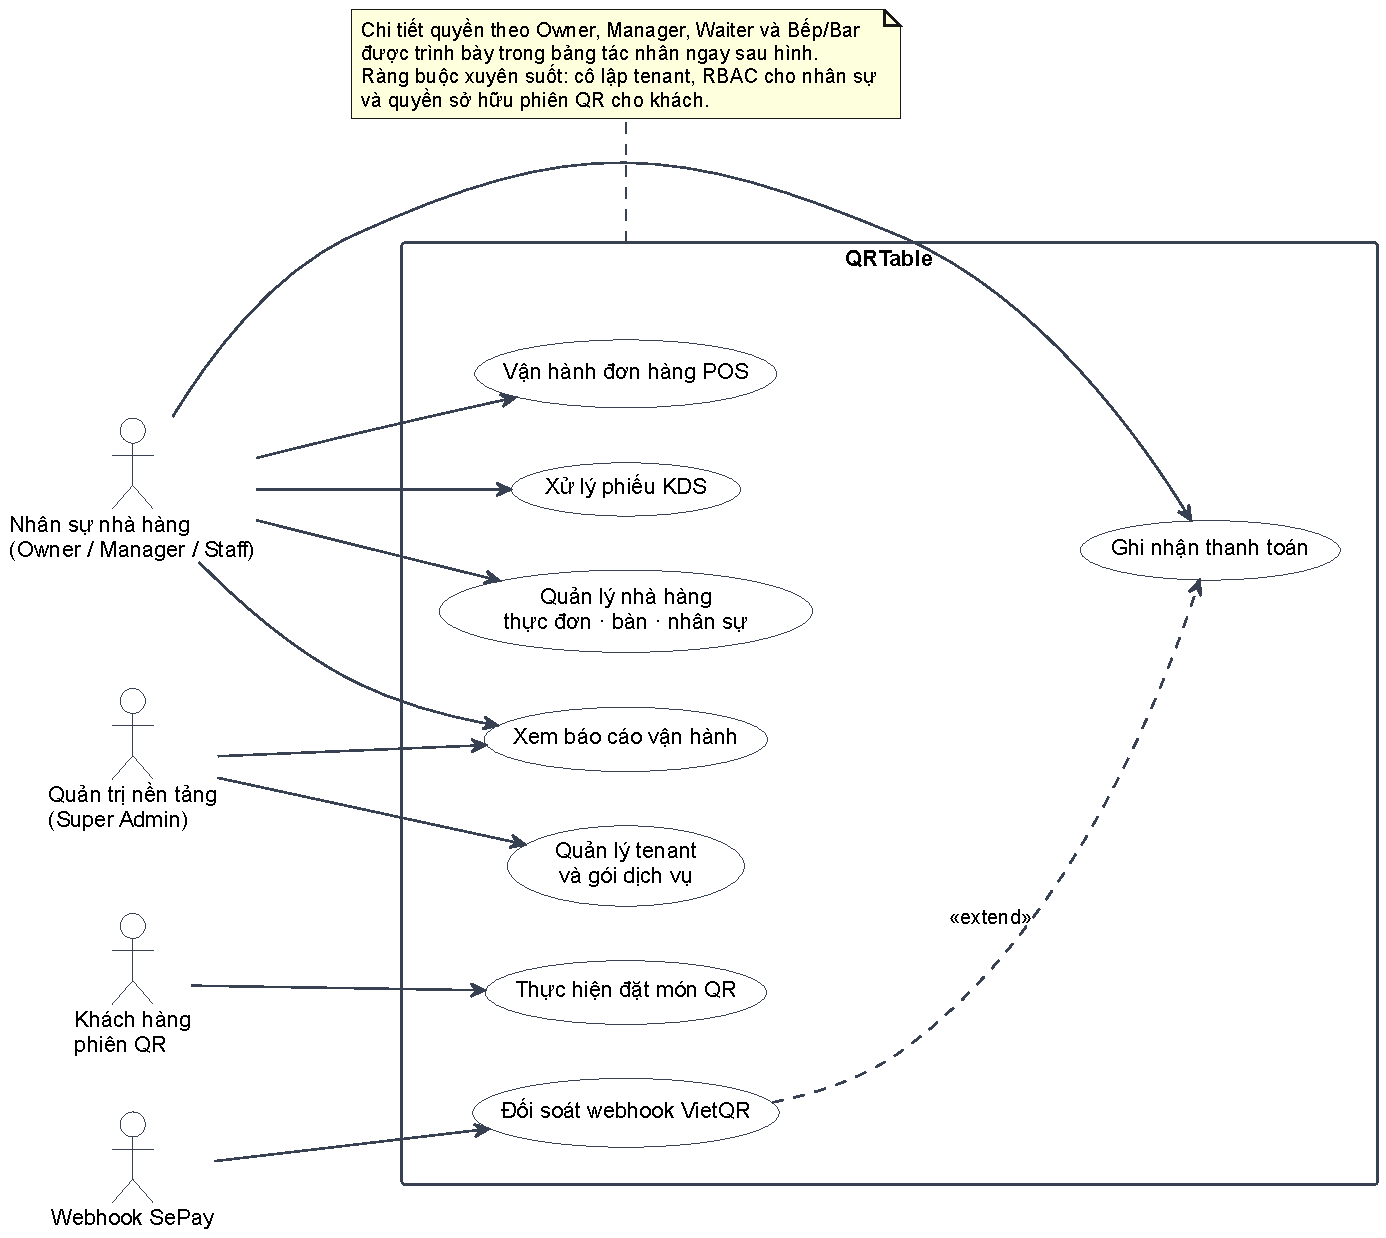
\includegraphics[width=\textwidth]{chapter3-actor-use-case-overview.pdf}
  \caption{Tổng quan tác nhân và nhóm trường hợp sử dụng chính của QRTable.}
  \label{fig:chapter3-actor-use-case-overview}
\end{figure}

\begin{longtable}{@{}>{\raggedright\arraybackslash}p{0.18\textwidth}>{\raggedright\arraybackslash}p{0.22\textwidth}>{\raggedright\arraybackslash}p{0.54\textwidth}@{}}
\caption{Tác nhân, phạm vi truy cập và trường hợp sử dụng chính của QRTable.}
\label{tab:chapter3-actors}\\
\toprule
\textbf{Tác nhân} & \textbf{Phạm vi} & \textbf{Trường hợp sử dụng chính} \\
\midrule
\endfirsthead
\toprule
\textbf{Tác nhân} & \textbf{Phạm vi} & \textbf{Trường hợp sử dụng chính} \\
\midrule
\endhead
Quản trị nền tảng & Toàn nền tảng, chéo tenant & Đưa tenant vào hệ thống, quản lý trạng thái tenant, quản lý gói giá, xem đăng ký/hóa đơn ở lớp nền tảng, hỗ trợ xác nhận hóa đơn gói dịch vụ khi cần, xem số liệu tổng hợp của nền tảng và xem chi tiết báo cáo theo tenant qua quyền \texttt{report.read\_any}. \\
\addlinespace
Chủ nhà hàng & Một tenant & Quản lý thực đơn, danh mục, bàn, QR, nhân sự, đơn, KDS, thanh toán, gói thuê bao của tenant; thanh toán gói; cập nhật cấu hình thanh toán; xem bảng điều khiển và báo cáo của tenant qua \texttt{report.read\_own} khi gói thuê bao đang hiệu lực và gói có \texttt{analytics\_basic}. \\
\addlinespace
Quản lý & Một tenant & Vận hành nhà hàng gần giống chủ quán ở lớp nghiệp vụ hằng ngày: quản lý thực đơn/bàn/đơn/KDS/thanh toán, quản lý nhân sự trong phạm vi được cấp và xem bảng điều khiển/báo cáo của tenant; không thanh toán gói, không cập nhật cấu hình thanh toán và không xóa người dùng. \\
\addlinespace
Phục vụ/POS & Một tenant, phạm vi sàn & Xem đơn, xác nhận hoặc hủy đơn chờ xử lý, xử lý thanh toán tiền mặt, xem lịch sử thanh toán, chuyển bàn, cập nhật trạng thái bàn và xử lý yêu cầu hỗ trợ. \\
\addlinespace
Bếp/Bar & Một tenant, theo trạm bếp/bar & Xem hàng đợi KDS theo trạm, cập nhật phiếu, thu hồi phiếu thao tác nhầm; không mặc định có quyền quản lý đầy đủ thực đơn, nhân sự, thanh toán hoặc POS. \\
\addlinespace
Khách hàng & Một phiên/bàn & Quét QR, tham gia hoặc tạo phiên, xem thực đơn công khai, thao tác giỏ chung, gửi đơn, theo dõi trạng thái đơn, yêu cầu hỗ trợ, yêu cầu thanh toán và thanh toán hóa đơn hiện tại. \\
\addlinespace
Webhook SePay & Hệ thống ngoài, theo mã thanh toán & Gửi sự kiện thanh toán cho hóa đơn nhà hàng hoặc hóa đơn gói dịch vụ; không phải tác nhân người dùng và phải đi qua tuyến xác minh tương ứng. \\
\bottomrule
\end{longtable}

Các trường hợp sử dụng của quản trị nền tảng thuộc lớp nền tảng, không nằm trong tenant vận hành hằng ngày. Quản trị nền tảng có thể tạo tenant, quản lý vòng đời tenant và quản lý gói dịch vụ. Tuy nhiên, các thao tác vận hành nhà hàng thông thường vẫn thuộc chủ quán, quản lý và nhân viên trong tenant. Điều này giúp tránh tình trạng một tác nhân nền tảng bị mô tả như nhân viên vận hành của từng nhà hàng.

Chủ nhà hàng là tác nhân có phạm vi quyền rộng nhất trong tenant. Chủ quán chịu trách nhiệm thiết lập dữ liệu vận hành ban đầu như thực đơn, khu vực, bàn, mã QR, nhân sự và cấu hình thanh toán. Chủ quán cũng có quyền thực hiện các thao tác nhạy cảm với gói thuê bao SaaS và cấu hình thanh toán của tenant. Quản lý có quyền vận hành mạnh nhưng bị giới hạn ở các thao tác có rủi ro tài chính hoặc quản trị nhân sự, ví dụ không được thanh toán gói, không được cập nhật cấu hình thanh toán và không được xóa người dùng. Đây là ranh giới quan trọng để chương thiết kế sau này giải thích RBAC và chuỗi bộ kiểm soát (guard).

Nhân viên phục vụ tập trung vào luồng POS: nhận thông báo đơn chờ xử lý, xác nhận đơn, xử lý hủy đơn chờ, quản lý bàn, chuyển bàn và thanh toán. Bếp/bar tập trung vào KDS, tức xem hàng đợi và cập nhật phiếu theo trạm. Hai nhóm này đều là nhân sự của tenant nhưng có trách nhiệm khác nhau; việc tách phục vụ khỏi bếp/bar giúp yêu cầu hệ thống phản ánh đúng luồng phối hợp giữa sàn phục vụ và bếp/quầy. Theo ma trận quyền hiện tại, Waiter, Chef và Barista không mặc định có quyền xem báo cáo doanh thu hoặc bảng điều khiển báo cáo.

Khách hàng là tác nhân theo phạm vi phiên. Khách không đăng nhập bằng Keycloak, không có vai trò trong ma trận quyền và không được truy cập dữ liệu ngoài phiên/bàn của mình. Các yêu cầu của khách xoay quanh trải nghiệm thuận tiện: quét QR, xem thực đơn, cùng bàn thao tác trên giỏ hàng chung, gửi đơn, theo dõi trạng thái và thanh toán. Các kiểm soát bảo mật đối với khách vì vậy phải dựa trên token QR, guard phiên, quyền sở hữu tenant/bàn/phiên và trạng thái bàn.

\section{Năng lực hệ thống theo các miền vận hành}

Các yêu cầu chức năng được nhóm theo miền nghiệp vụ để giữ ranh giới phân tích rõ ràng. Cách nhóm này giúp tránh mô tả yêu cầu theo màn hình client hoặc theo triển khai dịch vụ quá sớm. Trong Chương 4 và Chương 5, các miền này được ánh xạ sang ranh giới dịch vụ, trách nhiệm dữ liệu và bằng chứng triển khai.

\begin{longtable}{@{}>{\raggedright\arraybackslash}p{0.10\textwidth}>{\raggedright\arraybackslash}p{0.16\textwidth}>{\raggedright\arraybackslash}p{0.43\textwidth}>{\raggedright\arraybackslash}p{0.21\textwidth}@{}}
\caption{Yêu cầu chức năng theo miền nghiệp vụ.}
\label{tab:chapter3-functional-requirements}\\
\toprule
\textbf{ID} & \textbf{Miền} & \textbf{Yêu cầu chức năng} & \textbf{Tiêu chí kiểm soát} \\
\midrule
\endfirsthead
\toprule
\textbf{ID} & \textbf{Miền} & \textbf{Yêu cầu chức năng} & \textbf{Tiêu chí kiểm soát} \\
\midrule
\endhead
FR-SAAS-01 & Đưa tenant vào hệ thống & Hệ thống phải hỗ trợ đưa tenant vào theo hướng có quản trị hỗ trợ: tạo tenant, chủ quán ban đầu, gói thuê bao mặc định và bản ghi cấu hình thanh toán trong một quy trình nhất quán. & Tạo tenant không để lại dữ liệu mồ côi khi một bước con thất bại; chủ quán được gắn đúng tenant. \\
\addlinespace
FR-SAAS-02 & Vòng đời tenant và gói thuê bao & Hệ thống phải quản lý trạng thái tenant, gói giá, gói thuê bao đang hiệu lực, hóa đơn gói và hạn mức như số bàn, số nhân viên, số đơn/ngày. & Một tenant chỉ có một gói thuê bao đang hiệu lực; tenant bị tạm ngưng bị giới hạn thao tác mới nhưng vẫn xử lý được luồng thanh toán đã phát sinh. \\
\addlinespace
FR-USER-01 & Quản lý nhân sự tenant & Chủ quán và quản lý phải quản lý nhân sự của tenant theo quyền được cấp; chủ quán có quyền thao tác nhạy hơn như xóa người dùng hoặc cập nhật vai trò, còn quản lý không được xóa người dùng. & Quản lý nhân sự thuộc phạm vi tenant, không phụ thuộc dịch vụ thông báo hoặc gửi email; không mở rộng thành quản trị nhân sự nâng cao (HRM), bảng lương hoặc lập ca. \\
\addlinespace
FR-CAT-01 & Thực đơn & Chủ quán và quản lý phải quản lý danh mục, món, ảnh, thứ tự hiển thị và trạng thái còn hàng hoặc hết hàng; khách và nhân viên chỉ xem dữ liệu thực đơn phù hợp với tenant. & Thực đơn công khai chỉ hiển thị danh mục đang hoạt động và món còn bán, chưa bị xóa. \\
\addlinespace
FR-CAT-02 & Bàn và QR & Hệ thống phải quản lý khu vực, bàn, trạng thái bàn và token QR theo phạm vi tenant/bàn để khách vào đúng phiên. & Token QR không hợp lệ hoặc không khớp tenant/bàn phải bị từ chối. \\
\addlinespace
FR-ORD-01 & Phiên và giỏ chung & Khách cùng bàn phải dùng chung phiên/giỏ; các thao tác giỏ hàng phải kiểm soát phiên bản để tránh ghi đè khi nhiều thiết bị cùng thao tác. & Cập nhật giỏ lỗi thời bị từ chối và phía client phải lấy lại ảnh chụp trạng thái từ máy chủ. \\
\addlinespace
FR-ORD-02 & Gửi đơn & Gửi đơn phải tạo đơn chờ xử lý một lần theo khóa idempotency, không tạo bản nháp đơn trong cơ sở dữ liệu và xóa giỏ sau khi gửi thành công. & Gửi lặp cùng khóa idempotency không tạo đơn trùng. \\
\addlinespace
FR-ORD-03 & Xác nhận đơn và tồn kho & Nhân viên/chủ quán/quản lý phải xác nhận đơn chờ trước khi món vào bếp; tồn kho chỉ được trừ tại thời điểm xác nhận và thuộc quyền kiểm soát của miền Thực đơn (Catalog). & Đơn không được cập nhật trực tiếp dữ liệu tồn kho của Catalog; lỗi thiếu hàng phải trả về có cấu trúc cho nhân viên. \\
\addlinespace
FR-ORD-04 & Chính sách hủy & Khách chỉ được hủy đơn chờ thuộc phiên của mình; nhân viên được hủy đơn chờ; chủ quán/quản lý được hủy đơn đang xử lý với lý do và chính sách tồn kho phù hợp. & Không cho khách hủy đơn đã vào bếp; hủy đơn phải giữ vết nghiệp vụ. \\
\addlinespace
FR-ORD-05 & Hóa đơn và yêu cầu hỗ trợ & Khách có thể yêu cầu hỗ trợ và yêu cầu thanh toán; yêu cầu hóa đơn chỉ hợp lệ khi giỏ rỗng và các đơn đang hoạt động đã ở trạng thái phục vụ xong. & Khi hóa đơn chờ thanh toán, hệ thống khóa giỏ và chuyển bàn sang trạng thái thanh toán. \\
\addlinespace
FR-KDS-01 & Bếp/KDS & Miền bếp phải nhận phiếu từ đơn đã xác nhận, tách theo trạm bếp/bar, chống trùng phiếu theo tenant, đơn và trạm. & Hàng đợi KDS hiển thị đúng trạm và không tạo phiếu trùng khi nhận sự kiện lặp. \\
\addlinespace
FR-KDS-02 & Thao tác KDS & Bếp/bar phải xem hàng đợi FIFO, cập nhật trạng thái phiếu, thu hồi thao tác nhầm, nhận cảnh báo SLA và tín hiệu thời gian thực để làm mới dữ liệu. & WebSocket chỉ là tín hiệu cập nhật; ảnh chụp trạng thái vẫn lấy từ phía máy chủ. \\
\addlinespace
FR-PAY-01 & Quyết toán thanh toán & Hệ thống phải hỗ trợ thanh toán tiền mặt và VietQR/SePay cho hóa đơn nhà hàng, dùng mã thanh toán ổn định và quy tắc làm tròn VND. & Webhook thiếu tiền không đóng hóa đơn; webhook trùng không làm thanh toán bị ghi nhận nhiều lần. \\
\addlinespace
FR-PAY-02 & Lịch sử thanh toán và đối soát & Chủ quán/quản lý xem lịch sử thanh toán theo tenant ở chế độ chỉ đọc để đối soát vận hành; điều chỉnh sau thanh toán không thuộc phạm vi luận văn. & Dữ liệu lịch sử phải được lọc theo tenant; không cho phép sửa trạng thái thanh toán từ màn hình lịch sử. \\
\addlinespace
FR-DASH-01 & Báo cáo tenant & Chủ quán và quản lý phải xem được báo cáo tenant cho doanh thu, đơn hàng, bàn, thực đơn và thanh toán ở mức tổng hợp. & Yêu cầu {\scriptsize\texttt{report.read\_own}}, gói thuê bao ở trạng thái {\scriptsize\texttt{ACTIVE}} và mã tính năng {\scriptsize\texttt{analytics\_basic}}; thành phần báo cáo bị khóa theo gói không được gọi API báo cáo. \\
\addlinespace
FR-DASH-02 & Phân tích số liệu nền tảng & Quản trị nền tảng phải xem được số liệu tổng hợp của nền tảng và xem chi tiết báo cáo tenant khi cần hỗ trợ/đối soát. & Yêu cầu {\scriptsize\texttt{report.read\_any}}; kết quả của quản trị nền tảng không bị khóa bởi gói dịch vụ của tenant được chọn. \\
\addlinespace
FR-RBAC-01 & Xác thực/RBAC & API được bảo vệ phải được kiểm soát bằng chuỗi guard, ngữ cảnh tenant và ma trận quyền; điều hướng client chỉ hỗ trợ trải nghiệm người dùng, không thay thế kiểm soát ở phía máy chủ. & API phải từ chối tác nhân thiếu quyền hoặc sai tenant ngay cả khi client bị bỏ qua. \\
\bottomrule
\end{longtable}

Nhóm yêu cầu SaaS xác định QRTable là nền tảng nhiều nhà hàng, không phải phần mềm cài riêng cho từng nhà hàng. Do đó, việc tạo tenant, gắn chủ quán, quản lý gói thuê bao và hạn mức là yêu cầu nền tảng. Trạng thái tenant cũng ảnh hưởng trực tiếp tới luồng khách: tenant bị tạm ngưng không nên tiếp nhận thao tác mới tùy tiện, nhưng các luồng thanh toán đã tạo trước đó cần được xử lý an toàn để không làm thất thoát giao dịch.

Nhóm yêu cầu nhân sự được giới hạn ở quản lý nhân sự trong tenant. Chủ quán và quản lý có thể quản lý nhân sự theo ma trận phân quyền, trong đó chủ quán có quyền thao tác nhạy hơn như xóa người dùng hoặc cập nhật vai trò, còn quản lý bị giới hạn ở các thao tác vận hành được cấp. Phạm vi này không bao gồm quy trình quản trị nhân sự nâng cao (HRM) như bảng lương, ca làm, chấm công hoặc phụ thuộc vào dịch vụ email/thông báo.

Nhóm thực đơn, bàn và QR xác định điểm vào vật lý của khách hàng. Mỗi mã QR phải gắn với đúng tenant và bàn. Thực đơn công khai cần tôn trọng trạng thái danh mục/món để khách chỉ thấy các món đang được phép bán. Các thao tác thay đổi thực đơn hoặc bàn thuộc chủ quán/quản lý, trong khi khách không có quyền quản lý thực đơn. Đây là nền cho yêu cầu cô lập tenant: cùng một hệ thống có nhiều tenant nhưng thực đơn, bàn và QR của tenant này không được lẫn với tenant khác.

Nhóm phiên, giỏ và đơn là lõi của đặt món qua QR. Một bàn có thể có nhiều khách cùng thao tác, nên giỏ hàng phải được chia sẻ và có cơ chế chống ghi đè. Gửi đơn chỉ tạo đơn chính thức khi khách gửi, còn giỏ hàng trước đó là trạng thái tạm của phiên. Xác nhận của nhân viên là điểm chuyển từ mong muốn của khách sang cam kết vận hành của nhà hàng: tồn kho được kiểm tra và trừ tại đây, đơn chuyển sang đang xử lý và phiếu được gửi sang KDS. Quy tắc này giúp tránh trừ tồn kho quá sớm khi khách chỉ đang thêm món vào giỏ.

Nhóm KDS và thanh toán hoàn tất vòng đời vận hành. KDS cần ưu tiên tính đúng đắn của hàng đợi và trạm hơn là chỉ hiển thị thời gian thực. Thanh toán cần xử lý cả giao dịch do nhân viên xác nhận trực tiếp và giao dịch do webhook từ hệ thống ngoài gửi về. Vì webhook có thể đến trễ hoặc đến nhiều lần, yêu cầu idempotency là bắt buộc trong luồng thanh toán.

Nhóm bảng điều khiển và báo cáo bổ sung khả năng đọc hiểu vận hành sau khi dữ liệu giao dịch đã phát sinh. Trong phạm vi yêu cầu của QRTable, báo cáo là mô hình dữ liệu đọc chỉ đọc do các miền sở hữu dữ liệu cung cấp, ví dụ miền Thanh toán cho doanh thu đã thanh toán, miền Đơn cho đơn/hóa đơn, miền Thực đơn cho bàn/thực đơn và miền SaaS cho số liệu nền tảng. Chương 3 vì vậy xác định nhu cầu đọc tổng hợp và quyền truy cập báo cáo, còn dịch vụ phân tích riêng, kho dữ liệu OLAP hoặc quy trình phân tích nghiệp vụ chuyên sâu thuộc nhóm mở rộng sản phẩm.

Hình~\ref{fig:chapter3-business-flow} gom các yêu cầu chức năng trên thành một luồng nghiệp vụ xuyên suốt từ lúc khách quét QR cho đến khi bàn được dọn và sẵn sàng phục vụ lượt tiếp theo. Trong Chương 3, luồng này thể hiện trình tự nghiệp vụ và điều kiện kiểm soát chính; trình tự chi tiết giữa các dịch vụ được trình bày ở Chương 5.

\begin{figure}[htbp]
  \centering
  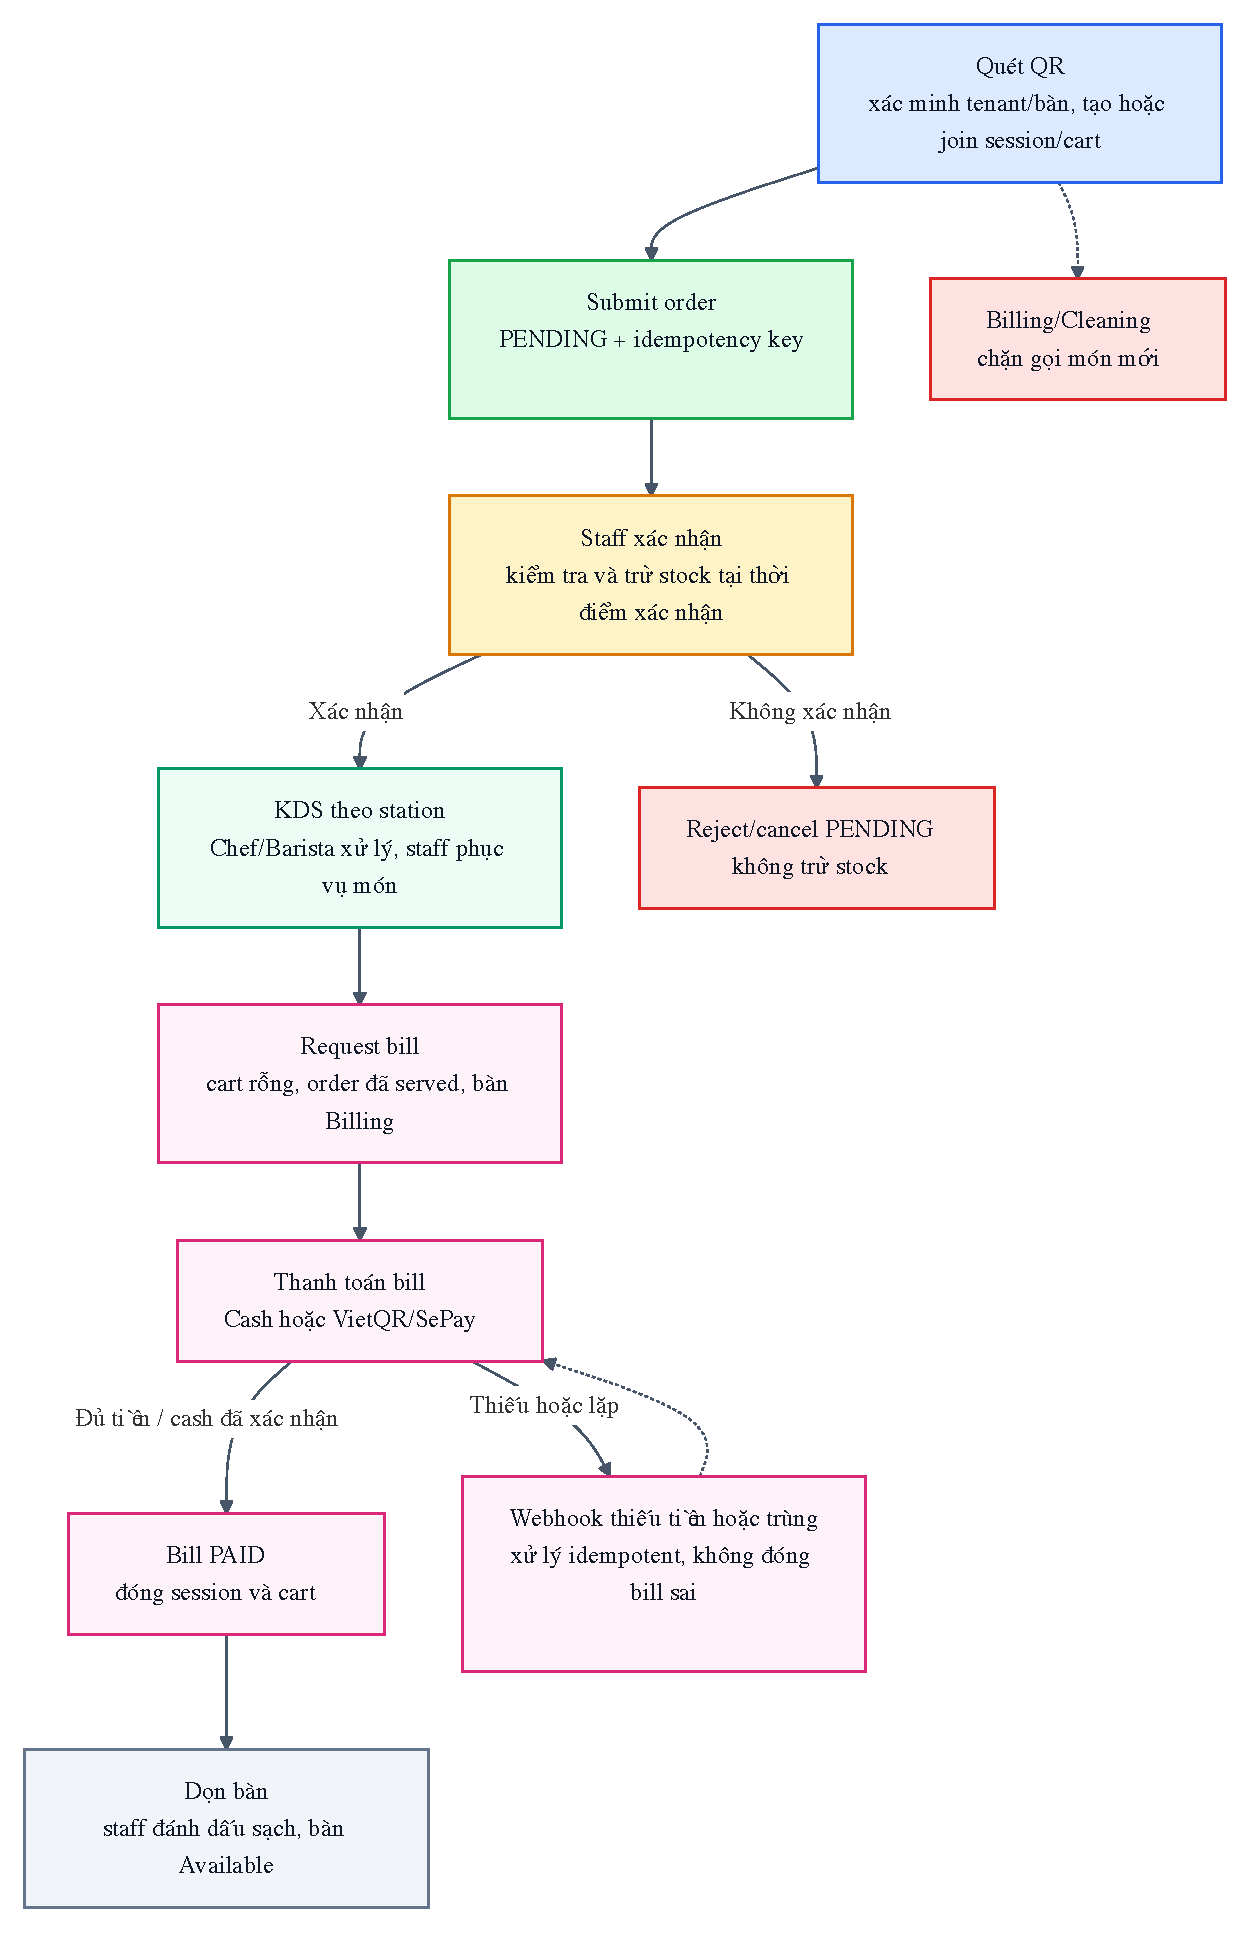
\includegraphics[width=\textwidth,height=0.82\textheight,keepaspectratio]{chapter3-business-flow.pdf}
  \caption{Luồng nghiệp vụ từ đặt món qua QR đến KDS, thanh toán và dọn bàn.}
  \label{fig:chapter3-business-flow}
\end{figure}

\section{Ràng buộc chất lượng và tiêu chí kiểm chứng}

Các yêu cầu phi chức năng của QRTable được diễn đạt dựa trên đặc thù hệ thống SaaS nhiều tenant và các thuộc tính chất lượng thường dùng trong đánh giá hệ thống phần mềm như bảo mật, độ tin cậy, khả năng bảo trì và hiệu năng \cite{iso-iec-25010-2023}. Trong phạm vi khóa luận, các yêu cầu này đóng vai trò tiêu chí thiết kế và đánh giá có kiểm soát ở Chương 4, Chương 5 và Chương 6.

\begin{longtable}{@{}>{\raggedright\arraybackslash}p{0.16\textwidth}>{\raggedright\arraybackslash}p{0.44\textwidth}>{\raggedright\arraybackslash}p{0.34\textwidth}@{}}
\caption{Yêu cầu phi chức năng và tiêu chí đánh giá.}
\label{tab:chapter3-non-functional-requirements}\\
\toprule
\textbf{YC phi chức năng} & \textbf{Yêu cầu} & \textbf{Cách đánh giá an toàn} \\
\midrule
\endfirsthead
\toprule
\textbf{YC phi chức năng} & \textbf{Yêu cầu} & \textbf{Cách đánh giá an toàn} \\
\midrule
\endhead
Cô lập tenant & Dữ liệu, API, khóa cache, tải trọng sự kiện và tệp tải lên liên quan tenant phải luôn được ràng buộc bởi ngữ cảnh tenant. & Đánh giá bằng kiểm thử dịch vụ, kiểm thử guard, ma trận truy vết và kịch bản tenant A/B đại diện. \\
\addlinespace
Bảo mật và phân quyền & Nhân viên/chủ quán/quản trị dùng JWT/OIDC và RBAC; khách dùng xác thực theo phạm vi QR/phiên; cấu hình webhook/thanh toán không được lộ khóa bí mật hoặc token ra trình duyệt. & Đánh giá bằng ma trận quyền, chuỗi guard, hợp đồng tuyến API và kịch bản bảo mật cho QR/webhook. \\
\addlinespace
Nhất quán và idempotency & Các luồng ghi ảnh hưởng trạng thái tiền hoặc đơn phải có idempotency và nguồn trạng thái đáng tin rõ ràng: gửi đơn, xác nhận tồn kho, quyết toán webhook, đánh dấu hóa đơn đã thanh toán. & Đánh giá bằng kiểm thử máy trạng thái, kiểm thử tích hợp và kịch bản phát lại/trùng lặp. \\
\addlinespace
Phản hồi thời gian thực & Hệ thống cần phản hồi kịp thời cho POS, KDS và PWA khách, trong đó sự kiện thời gian thực đóng vai trò gợi ý hoặc làm mất hiệu lực bộ nhớ đệm. & Kiểm tra client nhận gợi ý rồi lấy lại ảnh chụp trạng thái; nguồn trạng thái nghiệp vụ cuối cùng vẫn nằm ở phía máy chủ. \\
\addlinespace
Khả năng bảo trì & Hệ thống cần có ranh giới miền rõ, hợp đồng dùng chung ổn định và cấu trúc monorepo hỗ trợ thay đổi có kiểm soát. & Đánh giá bằng trách nhiệm dịch vụ, thư viện dùng chung, hợp đồng kiến trúc và khả năng truy vết yêu cầu sang module liên quan. \\
\addlinespace
Khả năng mở rộng & Kiến trúc cần cho phép mở rộng theo ranh giới dịch vụ, bộ nhớ đệm, nhóm consumer hoặc bộ chuyển đổi thời gian thực khi cần. & Đánh giá bằng lập luận kiến trúc và bằng chứng ranh giới dịch vụ; phép đo tải lớn thuộc lớp kiểm chứng thực nghiệm với môi trường và dữ liệu riêng. \\
\addlinespace
Khả kiểm thử và minh họa tái lập được & Yêu cầu ưu tiên cao cần có ánh xạ sang kiểm thử, kịch bản minh họa hoặc tư liệu bằng chứng để người đọc kiểm tra được luận điểm. & Đánh giá bằng ma trận truy vết, kết quả kiểm thử, ảnh chụp/tư liệu minh họa và danh sách kiểm tra quá trình build. \\
\bottomrule
\end{longtable}

Cô lập tenant là yêu cầu phi chức năng trung tâm vì QRTable phục vụ nhiều nhà hàng trên cùng nền tảng. Cô lập không chỉ nằm ở truy vấn cơ sở dữ liệu mà còn ở khóa cache, phòng WebSocket, token QR, tệp tải lên, mã thanh toán và guard phân quyền. Nếu một API hoặc khóa cache bỏ qua ngữ cảnh tenant, dữ liệu của tenant này có thể bị lộ sang tenant khác. Vì vậy, mọi yêu cầu chức năng ở trên đều phải được đọc cùng yêu cầu cô lập.

Bảo mật của QRTable có hai mặt khác nhau. Với nhân viên, chủ quán, quản lý và quản trị nền tảng, hệ thống cần xác thực bằng JWT/OIDC và ủy quyền bằng RBAC. Với khách, hệ thống cần tối ưu trải nghiệm quét QR nên không yêu cầu tài khoản Keycloak; thay vào đó, quyền truy cập được giới hạn bằng quyền sở hữu QR/phiên/bàn. Với webhook thanh toán, yêu cầu bảo mật nằm ở xác minh tuyến, khóa bí mật/HMAC, mã thanh toán và idempotency. Ba nhóm cơ chế này được tách biệt khi thiết kế và đánh giá.

Nhất quán và idempotency xuất hiện ở các điểm có rủi ro cao: nhiều khách cùng sửa giỏ chung, khách gửi đơn nhiều lần do thử lại, nhân viên xác nhận đơn trong khi tồn kho thay đổi, webhook SePay gửi lặp, hoặc sự kiện thanh toán được phát lại để đồng bộ sang miền Đơn. Yêu cầu hệ thống là xác định rõ mỗi trạng thái do miền nào sở hữu, thao tác nào cần idempotency và thao tác lặp có tạo tác dụng phụ trùng lặp hay không.

Phản hồi thời gian thực giúp trải nghiệm vận hành mượt hơn trong khi nguồn trạng thái có thẩm quyền vẫn nằm ở phía máy chủ. POS, KDS và PWA khách nhận gợi ý WebSocket để biết thời điểm làm mới dữ liệu; trạng thái cuối cùng được lấy từ ảnh chụp trạng thái phía máy chủ. Cách diễn đạt này giữ rõ vai trò của WebSocket mà không phóng đại tính đúng đắn của đơn, phiếu bếp hoặc thanh toán.

\section{Các vòng đời trạng thái chi phối nghiệp vụ}

QRTable có nhiều máy trạng thái nghiệp vụ liên kết với nhau. Bàn, phiên, giỏ, đơn, phiếu KDS, hóa đơn/thanh toán và tenant đều có vòng đời riêng. Một yêu cầu quan trọng là không để một trạng thái ở miền này bị cập nhật tùy tiện bởi miền khác. Ví dụ, thanh toán hoàn tất có thể kích hoạt việc đóng hóa đơn và chuyển bàn sang trạng thái dọn dẹp, nhưng không có nghĩa miền Thanh toán tự sở hữu toàn bộ vòng đời bàn; tương tự, đơn xác nhận món có thể yêu cầu miền Thực đơn trừ tồn kho, nhưng miền Đơn không sở hữu dữ liệu tồn kho.

\begin{longtable}{@{}>{\raggedright\arraybackslash}p{0.17\textwidth}>{\raggedright\arraybackslash}p{0.35\textwidth}>{\raggedright\arraybackslash}p{0.42\textwidth}@{}}
\caption{Tóm tắt các máy trạng thái nghiệp vụ chính của QRTable.}
\label{tab:chapter3-state-machines}\\
\toprule
\textbf{Máy trạng thái} & \textbf{Trạng thái chính} & \textbf{Quy tắc chuyển trạng thái quan trọng} \\
\midrule
\endfirsthead
\toprule
\textbf{Máy trạng thái} & \textbf{Trạng thái chính} & \textbf{Quy tắc chuyển trạng thái quan trọng} \\
\midrule
\endhead
Vòng đời tenant & \texttt{ACTIVE}, \texttt{SUSPENDED}, \texttt{CLOSED} & Quản trị nền tảng quản lý vòng đời; tạm ngưng giới hạn thao tác mới nhưng vẫn cho xử lý luồng thanh toán đã phát sinh; đóng là trạng thái kết thúc hợp đồng trong phạm vi hiện tại. \\
\addlinespace
Vòng đời gói thuê bao & Hóa đơn nháp/đã phát hành, gói đang hiệu lực, gói hết hạn/thay thế & Một tenant chỉ có một gói đang hiệu lực; hóa đơn gói dùng mã tham chiếu \texttt{QRSUB}; hạn mức áp cho bàn, nhân viên và số đơn/ngày. \\
\addlinespace
Vòng đời bàn/phiên & Trống, có khách, thanh toán, dọn dẹp; phiên đang hoạt động/đã đóng & Quét QR tạo hoặc tham gia phiên khi bàn trống/có khách; thanh toán và dọn dẹp chặn đơn mới; giải phóng phiên rỗng an toàn chỉ hợp lệ khi miền Đơn chứng minh phiên rỗng. \\
\addlinespace
Vòng đời giỏ/đơn & Giỏ nháp, \texttt{PENDING}, \texttt{PROCESSING}, \texttt{READY}, \texttt{SERVED}, hoàn tất/hủy & Giỏ nháp không phải đơn lưu trong CSDL; gửi đơn tạo đơn chờ một lần; nhân viên xác nhận mới trừ tồn kho; khách chỉ hủy đơn chờ của phiên mình. \\
\addlinespace
Vòng đời phiếu KDS & Chờ, đang xử lý, sẵn sàng/xong, thu hồi & Phiếu sinh từ đơn đã xác nhận, tách theo trạm, sắp xếp theo FIFO/ưu tiên/SLA; thu hồi dùng để sửa thao tác nhầm. \\
\addlinespace
Vòng đời hóa đơn/thanh toán & \texttt{OPEN}, \texttt{PENDING\_PAYMENT}, \texttt{PAID} & Yêu cầu hóa đơn cần giỏ rỗng và đơn đã phục vụ xong; thanh toán xong đóng hóa đơn/phiên và chuyển bàn sang dọn dẹp; webhook trùng phải idempotent. \\
\bottomrule
\end{longtable}

Vòng đời bàn/phiên là cầu nối giữa thế giới vật lý của nhà hàng và trạng thái phần mềm. Khi bàn trống và khách quét QR, hệ thống tạo phiên mới và đánh dấu bàn có khách. Khi bàn có khách và phiên còn hợp lệ, khách khác cùng bàn tham gia phiên hiện tại. Khi khách yêu cầu thanh toán, bàn chuyển sang trạng thái thanh toán để khóa gọi món mới. Sau khi thanh toán hoàn tất, bàn chuyển sang dọn dẹp để nhân viên dọn bàn, rồi mới trở lại trống. Quy tắc giải phóng phiên rỗng an toàn chỉ áp dụng khi có bằng chứng rằng phiên rỗng, không có hóa đơn và không có đơn đã lưu; nó không phải chức năng mở khóa cưỡng bức tùy tiện.

Vòng đời giỏ/đơn tách rõ trạng thái trước và sau khi gửi đơn. Trước khi gửi, khách chỉ thao tác trên giỏ của phiên. Sau khi gửi, hệ thống tạo đơn chờ để nhân viên xác nhận. Tồn kho không bị trừ khi khách mới gửi, vì đơn chờ vẫn có thể bị hủy hoặc bị từ chối do thiếu hàng. Tồn kho được xử lý tại thời điểm nhân viên xác nhận, khi đơn chuyển sang đang xử lý. Cách tách này phù hợp thực tế nhà hàng: khách gửi yêu cầu, nhân viên kiểm tra rồi bếp mới bắt đầu thực hiện.

Vòng đời KDS bắt đầu sau khi đơn được xác nhận. Phiếu cần được định tuyến tới bếp hoặc bar theo trạm của món. Bếp/bar thao tác trên phiếu để chuyển trạng thái, còn phục vụ/POS theo dõi món sẵn sàng để phục vụ. KDS có thể nhận gợi ý thời gian thực để màn hình cập nhật nhanh hơn, nhưng hàng đợi phiếu và trạng thái đơn vẫn phải dựa vào ảnh chụp trạng thái phía máy chủ.

Vòng đời hóa đơn/thanh toán kết thúc phiên bàn. Hóa đơn chỉ nên vào chờ thanh toán khi không còn giỏ đang mở và các đơn cần thanh toán đã sẵn sàng. Thanh toán tiền mặt do nhân viên xác nhận trực tiếp, còn VietQR/SePay được xác nhận qua webhook. Vì thanh toán liên quan tiền và đối soát, các trường hợp thiếu tiền, trùng lặp hoặc webhook sau khi đã thanh toán phải được xử lý idempotent. Sau khi hóa đơn đã thanh toán, phiên được đóng, dữ liệu giỏ/phiên tạm được dọn và bàn chuyển sang dọn dẹp.

\section{Phạm vi yêu cầu của QRTable}

Phạm vi yêu cầu của QRTable tập trung vào các năng lực cần thiết để một đơn vị thuê bao F\&B vận hành quy trình đặt món tại bàn: quản lý tenant và gói thuê bao, thực đơn, bàn và mã QR, phiên khách, giỏ món dùng chung, đơn hàng, KDS, thanh toán, phân quyền và báo cáo vận hành mức MVP. Các yêu cầu này là cơ sở để Chương 4 thiết kế ranh giới dịch vụ, Chương 5 trình bày các luồng triển khai và Chương 6 đánh giá mức đáp ứng.

Các năng lực mở rộng như quản trị nhân sự nâng cao, CRM/loyalty, kho dữ liệu phân tích, BI/AI, ứng dụng di động gốc, hàng đợi thao tác ngoại tuyến đầy đủ, tích hợp sâu với nền tảng giao đồ ăn, hoàn tiền phức tạp hoặc nhiều ngân hàng thanh toán đồng thời được tách khỏi phạm vi yêu cầu chính. Việc đặt ranh giới này giúp phần đánh giá tập trung vào các luồng cốt lõi thay vì mở rộng sang những miền sản phẩm cần thiết kế, triển khai và kiểm chứng riêng.

Đối với hiệu năng, khả năng mở rộng và kiểm chứng nhà cung cấp thanh toán, Chương 3 xác định tiêu chí yêu cầu để Chương 4, Chương 5 và Chương 6 lần lượt thiết kế, hiện thực và phân loại bằng chứng tương ứng. Các kết luận về tải lớn, độ trễ, thông lượng hoặc callback SePay/VietQR với nhà cung cấp thật được đặt trong lớp đánh giá bằng chứng ở Chương 6. Nhờ đó, yêu cầu thanh toán vẫn bao gồm webhook, mã tham chiếu, xử lý thiếu tiền và trùng lặp, nhưng không trộn lẫn kiểm thử nội bộ với minh chứng vận hành thật.

Tóm lại, Chương 3 đã xác định tác nhân, trường hợp sử dụng, yêu cầu chức năng, yêu cầu phi chức năng và các máy trạng thái chính của QRTable. Đây là cơ sở để Chương 4 giải thích thiết kế kiến trúc và ranh giới dịch vụ, Chương 5 chứng minh quá trình triển khai, và Chương 6 đánh giá mức độ đáp ứng yêu cầu mà không phóng đại kết quả.

\chapter{Thiết kế kiến trúc và quyết định công nghệ cho QRTable}

Chương này trình bày cách QRTable chuyển các yêu cầu ở Chương 3 thành ranh giới kiến trúc, trách nhiệm dịch vụ, trách nhiệm dữ liệu, cơ chế giao tiếp và lựa chọn công nghệ cụ thể. Trọng tâm của chương không phải là liệt kê công nghệ, mà là giải thích vì sao từng quyết định phù hợp với bài toán nền tảng POS theo mô hình SaaS cho F\&B, có đặt món qua mã QR, màn hình bếp KDS, thanh toán VietQR/SePay và quản trị nhiều đơn vị thuê bao.

QRTable được thiết kế theo hướng vi dịch vụ (microservices) có kiểm soát. Các tài liệu về microservices nhấn mạnh việc tách hệ thống theo năng lực nghiệp vụ, sở hữu dữ liệu riêng và giao tiếp qua hợp đồng rõ ràng \cite{lewis-fowler-microservices-2014}. Tuy nhiên, trong phạm vi khóa luận, vi dịch vụ cũng tạo thêm chi phí về giao tiếp mạng, tính nhất quán dữ liệu (consistency), kiểm thử tích hợp và chẩn đoán lỗi phân tán. Vì vậy, QRTable không dùng Kafka cho mọi tương tác, không xem WebSocket là nguồn trạng thái nghiệp vụ, và không tách dịch vụ chỉ vì lý do kỹ thuật. Ranh giới được chọn dựa trên tác nhân, ngữ cảnh giới hạn, trách nhiệm dữ liệu và luồng nghiệp vụ thật của hệ thống.

\section{Mục tiêu thiết kế và nguyên tắc kiến trúc}

Các quyết định kiến trúc của QRTable được dẫn dắt bởi sáu mục tiêu chính.

Thứ nhất, hệ thống cần tách trách nhiệm theo miền nghiệp vụ. Catalog sở hữu thực đơn, bàn và tồn kho; Order sở hữu phiên, giỏ, đơn và hóa đơn; Payment sở hữu thanh toán và cấu hình thanh toán; SaaS sở hữu vòng đời đơn vị thuê bao và gói thuê bao. Cách tách này giúp quy tắc nghiệp vụ có nơi đặt rõ ràng, đồng thời tránh việc một dịch vụ ghi trực tiếp cơ sở dữ liệu của dịch vụ khác.

Thứ hai, cô lập đơn vị thuê bao phải là mặc định. QRTable phục vụ nhiều nhà hàng trên cùng nền tảng, nên mọi thao tác của dữ liệu nhà hàng phải mang ngữ cảnh \texttt{tenant\_id}. Mô hình hiện tại kết hợp cơ sở dữ liệu riêng theo dịch vụ với cột phân biệt \texttt{tenant\_id}. Cách tiếp cận này chưa phải mức cô lập vật lý cao nhất như cơ sở dữ liệu riêng cho từng đơn vị thuê bao, nhưng phù hợp với phạm vi hiện tại vì giảm chi phí vận hành, giữ quá trình thay đổi lược đồ dữ liệu đơn giản và vẫn cho phép kiểm soát dữ liệu theo đơn vị thuê bao ở API, cơ sở dữ liệu, Redis, Kafka và WebSocket. Khái niệm SaaS và chia sẻ tài nguyên nền tảng cũng làm cô lập đơn vị thuê bao trở thành một yêu cầu thiết kế cốt lõi \cite{nist-sp800145-2011}.

Thứ ba, BFF (Backend For Frontend) là điểm vào duy nhất của các ứng dụng phía người dùng. PWA khách và ứng dụng quản trị không gọi trực tiếp các dịch vụ nội bộ. BFF chịu trách nhiệm định tuyến HTTP, chuỗi guard bảo vệ, kiểm tra ngữ cảnh đơn vị thuê bao, cổng WebSocket và các thành phần gọi TCP/gRPC đến dịch vụ miền nghiệp vụ. Quyết định này giúp gom các mối quan tâm xuyên suốt ở lớp biên, trong khi bất biến nghiệp vụ vẫn nằm ở dịch vụ sở hữu.

Thứ tư, QRTable dùng giao tiếp hướng sự kiện có chọn lọc. TCP/gRPC được dùng cho lệnh hoặc truy vấn cần phản hồi ngay, chẳng hạn BFF gọi Order để gửi đơn hoặc Order gọi Catalog để trừ tồn kho khi nhân viên xác nhận. Kafka được dùng cho sự kiện miền nghiệp vụ và tác dụng phụ (side effect) bất đồng bộ, chẳng hạn \texttt{order.confirmed} để Kitchen tạo phiếu KDS hoặc \texttt{payment.completed} để Order hoàn tất hóa đơn. Cách dùng này tận dụng khả năng tách rời của Kafka \cite{apache-kafka-docs-2026} nhưng tránh biến bộ trung gian thông điệp thành tầng trung gian cho mọi thao tác phía client.

Thứ năm, Redis là bộ nhớ đệm (cache) và vùng trạng thái khi vận hành cho dữ liệu tần suất cao, không phải nguồn sự thật (source of truth) chung của hệ thống. Bộ nhớ đệm thực đơn công khai, phiên/giỏ khi vận hành, hàng đợi KDS, cờ tạm ngưng đơn vị thuê bao và trạng thái OAuth đều dùng Redis với chủ sở hữu rõ ràng. Với đơn, hóa đơn, thanh toán, đơn vị thuê bao và thực đơn, nguồn dữ liệu có thẩm quyền vẫn nằm ở dịch vụ sở hữu tương ứng.

Thứ sáu, các thao tác ghi ảnh hưởng đến trạng thái bên ngoài phải hướng tới idempotency (tính lũy đẳng), bù trừ có kiểm soát và dấu thời gian phía máy chủ. Điều này đặc biệt quan trọng ở webhook thanh toán, xác nhận đơn, xuất bản outbox và gửi đơn của khách. Trong phạm vi hiện tại, khóa luận xem saga pattern như thiết kế đại diện ở hai luồng: Order Confirm Saga cho xác nhận đơn/trừ tồn kho và SaaS Onboarding Mini-Saga cho khởi tạo đơn vị thuê bao (onboarding). Các tăng cường sâu hơn như trạng thái saga bền vững, tiến trình nền retry đầy đủ, CDC hoặc bảo đảm phân phối exactly-once được xem là hướng phát triển, không phải kết quả vận hành thực tế đã hoàn thiện.

\section{Lựa chọn công nghệ và vai trò trong QRTable}

Lựa chọn công nghệ trong QRTable xuất phát từ các mục tiêu thiết kế ở trên. Bảng~\ref{tab:chapter4-technology-decision} không nhằm so sánh đầy đủ mọi công nghệ thay thế; bảng này chỉ làm rõ công nghệ nào được dùng ở đâu, hỗ trợ mục tiêu nào và có giới hạn nào cần diễn đạt thận trọng. Riêng với Nx, tài liệu chính thức mô tả khả năng quản lý đồ thị dự án, xác định phần bị ảnh hưởng, bộ nhớ đệm tác vụ và thư viện dùng chung trong monorepo \cite{nx-docs-2026}; đây là lý do QRTable dùng Nx để quản lý nhiều ứng dụng và thư viện trong cùng kho mã nguồn.

{\footnotesize
\setlength{\tabcolsep}{3pt}
\begin{longtable}{>{\raggedright\arraybackslash}p{0.16\textwidth}>{\raggedright\arraybackslash}p{0.22\textwidth}>{\raggedright\arraybackslash}p{0.31\textwidth}>{\raggedright\arraybackslash}p{0.19\textwidth}}
  \caption{Quyết định công nghệ chính và vai trò trong QRTable.}
  \label{tab:chapter4-technology-decision}\\
  \toprule
  Công nghệ & Vị trí trong QRTable & Lý do sử dụng & Giới hạn cần lưu ý \\
  \midrule
  \endfirsthead
  \toprule
  Công nghệ & Vị trí trong QRTable & Lý do sử dụng & Giới hạn cần lưu ý \\
  \midrule
  \endhead
  \bottomrule
  \endfoot
  Nx monorepo & Quản lý \texttt{apps/} và \texttt{libs/} & Giữ ứng dụng, dịch vụ và hợp đồng dùng chung trong một kho mã nguồn; hỗ trợ phát hiện phụ thuộc và kiểm thử/xây dựng theo phần bị ảnh hưởng. & Monorepo không được làm mờ ranh giới dịch vụ hoặc cho phép nhập trực tiếp repository của dịch vụ khác. \\
  TypeScript và NestJS & BFF và các dịch vụ phía máy chủ & Tạo cấu trúc module/controller/service rõ ràng, thuận lợi cho DTO, guard, lớp tích hợp và hợp đồng TCP/gRPC/Kafka có kiểu. & Không thay thế được kiểm thử hợp đồng và quy tắc không truy cập chéo CSDL. \\
  Next.js và React & Ứng dụng quản trị & Phù hợp với client quản trị POS/KDS/báo cáo, nhiều trạng thái dữ liệu và luồng xác thực nhân viên. & Không biến client quản trị thành nơi quyết định nghiệp vụ; nghiệp vụ vẫn ở dịch vụ sở hữu. \\
  React/Vite PWA & Ứng dụng khách tại bàn & Tải nhanh cho luồng quét QR, xem thực đơn, giỏ chung và theo dõi đơn theo phiên. & Khách là tác nhân theo phiên, không dùng Keycloak như nhân viên. \\
  PostgreSQL & Dữ liệu nghiệp vụ quan hệ của nhiều dịch vụ & Phù hợp với đơn, hóa đơn, thực đơn, thanh toán, gói thuê bao và ràng buộc giao dịch nội bộ từng dịch vụ. & Không dùng một CSDL chung cho mọi dịch vụ; mỗi dịch vụ vẫn sở hữu dữ liệu của mình. \\
  MongoDB & User-Access & Lưu hồ sơ ứng dụng, vai trò và ánh xạ người dùng theo đơn vị thuê bao. & Không dùng MongoDB để thay thế nguồn danh tính Keycloak. \\
  Redis & Bộ nhớ đệm, phiên/giỏ khi vận hành, KDS và cờ trạng thái & Hỗ trợ TTL, dữ liệu tần suất cao và hàng đợi KDS bằng cấu trúc dữ liệu phù hợp. & Không là nguồn sự thật chung; mỗi nhóm khóa phải có chủ sở hữu rõ ràng. \\
  Kafka & Sự kiện miền bất đồng bộ & Tách thời gian giữa Order, Kitchen, Payment, SaaS và Catalog cho các tác dụng phụ không cần phản hồi ngay. & Chỉ dùng 5 topic được chấp nhận; không dùng Kafka cho mọi cập nhật phía client. \\
  Keycloak và JWT/OIDC & Xác thực nhân viên, chủ quán và quản trị & Tách nguồn định danh khỏi hồ sơ ứng dụng; BFF/Authorizer xác minh token, User-Access giữ thông tin ứng dụng. & Khách đặt món qua QR không đi qua Keycloak. \\
  Socket.IO\slash WebSocket & Gợi ý thời gian thực cho khách, nhân viên và KDS & Cải thiện trải nghiệm bằng thông báo, làm mất hiệu lực và gợi ý làm mới dữ liệu. & Không là nguồn trạng thái có thẩm quyền. \\
  SePay\slash VietQR và Cloudinary & Thanh toán chuyển khoản và ảnh thực đơn & SePay\slash VietQR phục vụ thanh toán hóa đơn/gói thuê bao; Cloudinary phục vụ tệp ảnh thực đơn. & Chỉ khẳng định kiểm chứng nhà cung cấp hoặc vận hành thực tế khi có bằng chứng tương ứng. \\
\end{longtable}
}

\section{Kiến trúc tổng thể và bản đồ tích hợp công nghệ}

Hình~\ref{fig:chapter4-technology-integration-map} là bản đồ đọc nhanh cho Chương 4. Hình đặt mỗi công nghệ vào đúng lớp kiến trúc: ứng dụng người dùng, lớp biên, dịch vụ miền nghiệp vụ, hạ tầng dữ liệu/sự kiện và nhà cung cấp ngoài. Các mũi tên không nhằm liệt kê mọi lời gọi trong mã nguồn, mà nhấn mạnh các luồng quyết định: ứng dụng chỉ đi qua BFF, dịch vụ giao tiếp nội bộ qua TCP/gRPC, Kafka chỉ dùng cho một số sự kiện miền, Redis chỉ giữ bộ nhớ đệm hoặc trạng thái chạy, còn webhook thanh toán đi qua BFF trước khi vào Payment hoặc SaaS.

\begin{figure}[H]
  \centering
  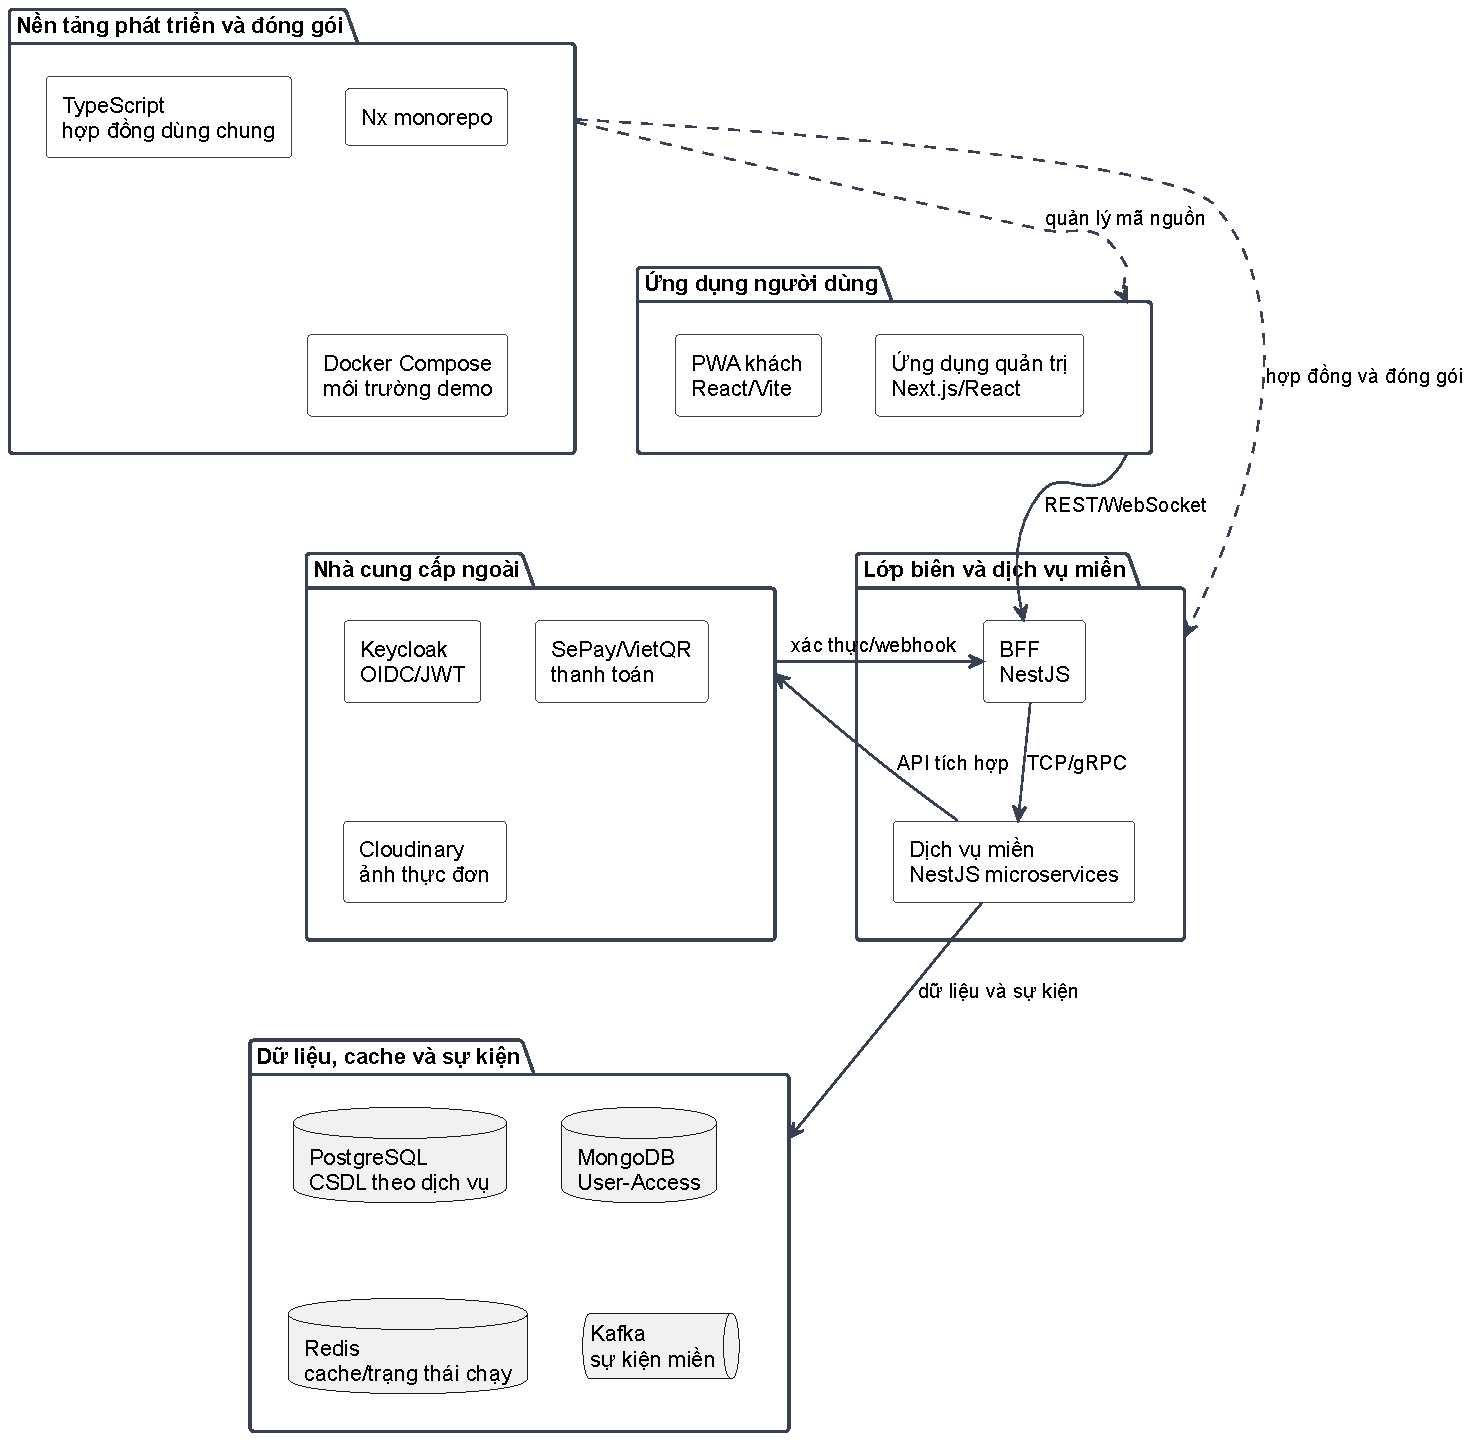
\includegraphics[width=\textwidth,height=0.82\textheight,keepaspectratio]{chapter4-technology-integration-map.pdf}
  \caption{Bản đồ tích hợp công nghệ trong kiến trúc QRTable.}
  \label{fig:chapter4-technology-integration-map}
\end{figure}

Hình~\ref{fig:chapter4-overall-architecture} tóm tắt kiến trúc tổng thể theo các lớp ứng dụng người dùng, BFF, dịch vụ miền nghiệp vụ và hạ tầng. Hình~\ref{fig:chapter4-c4-container} trình bày cùng hệ thống ở mức container theo C4 để làm rõ tác nhân, ứng dụng web, dịch vụ, kho lưu trữ (storage) và hệ thống ngoài. Trước khi đọc hai hình này, cần nắm ngắn gọn vai trò từng lớp như sau.

Ở lớp ứng dụng người dùng, QRTable có hai ứng dụng chính. PWA khách phục vụ khách tại bàn, bắt đầu từ thao tác quét mã QR, xem thực đơn, cập nhật giỏ chung, gửi đơn, theo dõi trạng thái và yêu cầu thanh toán. Ứng dụng quản trị phục vụ các tác nhân đã xác thực như quản trị nền tảng, chủ quán, quản lý, phục vụ, bếp và bar qua các vùng chức năng POS, KDS, bảng điều khiển và quản trị nền tảng.

Ở lớp biên, BFF là cửa vào duy nhất. BFF xử lý HTTP REST, WebSocket\slash Socket.IO, chuỗi guard và các thành phần gọi nội bộ đến dịch vụ miền nghiệp vụ. BFF có thể phát WebSocket hoặc làm mất hiệu lực bộ nhớ đệm sau khi nhận phản hồi từ dịch vụ, nhưng không sở hữu trạng thái nghiệp vụ như đơn, tồn kho, hóa đơn hoặc gói thuê bao.

Ở lớp dịch vụ miền nghiệp vụ, hệ thống gồm Authorizer, User-Access, SaaS, Catalog, Order, Kitchen và Payment. Mỗi dịch vụ đại diện cho một ngữ cảnh giới hạn: xác minh danh tính, hồ sơ ứng dụng/RBAC, vòng đời đơn vị thuê bao, thực đơn/bàn/tồn kho, đơn/phiên/hóa đơn, hàng đợi KDS và quyết toán thanh toán. Module \texttt{product} trong monorepo chỉ là phần mẫu do Nx sinh ra, không thuộc kiến trúc lõi QRTable vì không gánh trách nhiệm nghiệp vụ của hệ thống.

Ở lớp hạ tầng, QRTable dùng PostgreSQL cho dữ liệu nghiệp vụ quan hệ, MongoDB cho User-Access, Redis cho bộ nhớ đệm/phiên/hàng đợi KDS/cờ trạng thái chạy, Kafka cho sự kiện miền nghiệp vụ, Keycloak cho định danh nhân viên, SePay\slash VietQR cho thanh toán chuyển khoản, Cloudinary cho ảnh thực đơn và Docker\slash Docker Compose cho môi trường chạy.

\begin{figure}[H]
  \centering
  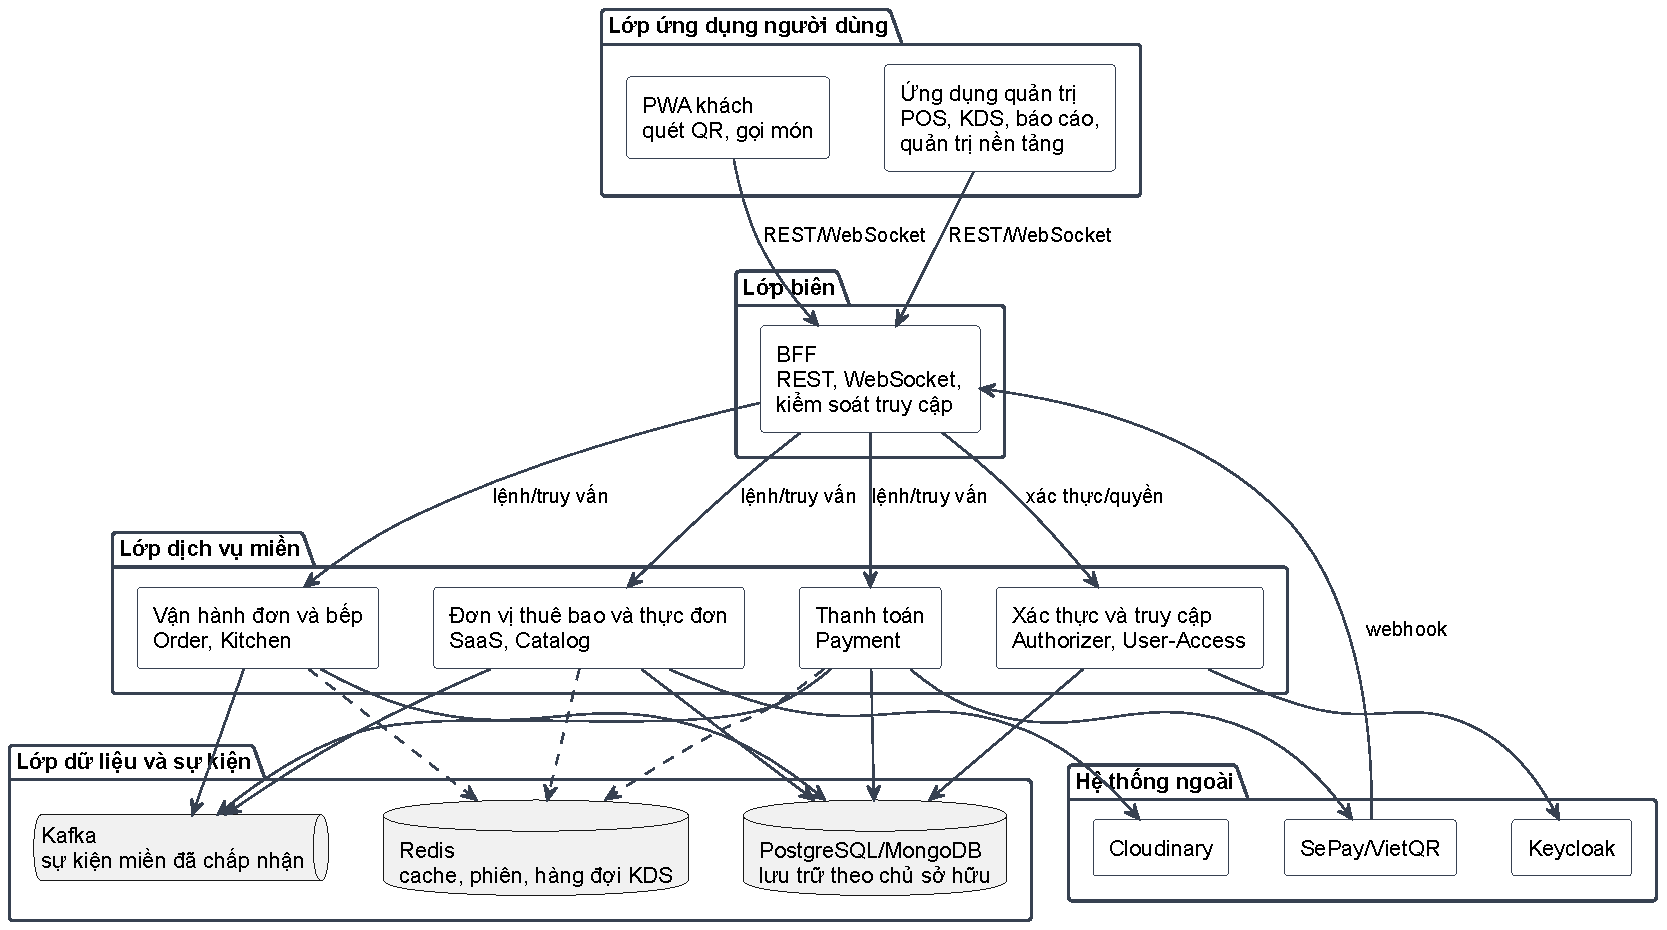
\includegraphics[width=\textwidth]{chapter4-overall-architecture.pdf}
  \caption{Kiến trúc tổng thể của QRTable.}
  \label{fig:chapter4-overall-architecture}
\end{figure}

\begin{figure}[H]
  \centering
  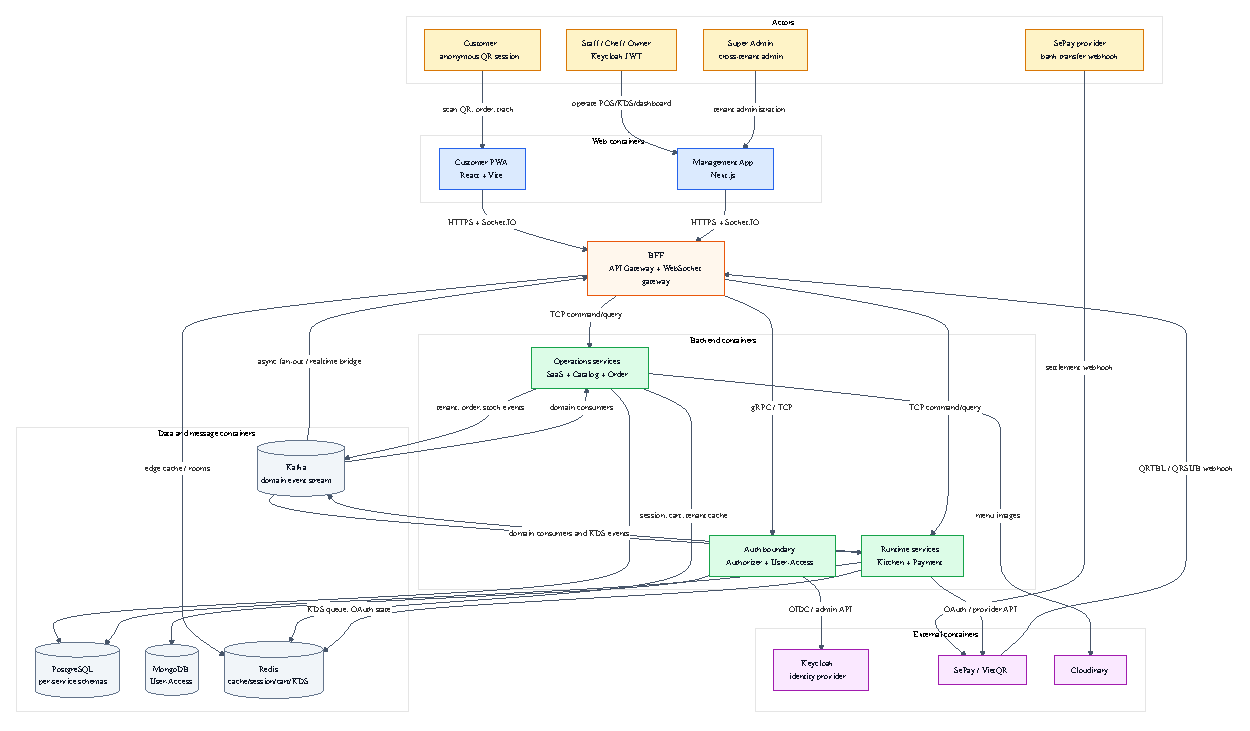
\includegraphics[width=\textwidth]{chapter4-c4-container.pdf}
  \caption{Sơ đồ container của QRTable theo góc nhìn C4.}
  \label{fig:chapter4-c4-container}
\end{figure}

\section{Tổ chức Nx monorepo và ranh giới mô-đun}

QRTable được tổ chức trong một kho mã nguồn Nx monorepo. Thư mục \texttt{apps/} chứa các đơn vị có thể triển khai như BFF, dịch vụ miền nghiệp vụ, PWA khách, ứng dụng quản trị và client Keycloak. Thư mục \texttt{libs/} chứa các thư viện chia sẻ như cấu hình, hằng số, DTO, guard, lớp tích hợp, hàng đợi, kiểu dùng chung, tiện ích, interface dùng chung và hook phía client.

Lý do dùng monorepo không phải để làm mờ ranh giới dịch vụ. Ngược lại, monorepo được dùng để giữ hợp đồng (contract) dùng chung ở một nơi có kiểm soát. Các phần như hằng số topic Kafka, bộ dựng khóa Redis, bộ dựng phòng WebSocket, DTO, interface, lớp tích hợp và guard có thể được nhập thống nhất thay vì định nghĩa lại ở từng dịch vụ. Điều này giảm nguy cơ lệch contract giữa BFF, dịch vụ và phía client khi hệ thống phát triển.

Một lợi ích khác của Nx là hỗ trợ đồ thị phụ thuộc và lệnh xác định phần bị ảnh hưởng (affected). Với hệ thống có nhiều ứng dụng và thư viện, thay đổi ở thư viện dùng chung có thể ảnh hưởng đến nhiều dự án con. Việc để các ứng dụng và thư viện trong cùng không gian làm việc Nx giúp phát hiện phụ thuộc rõ hơn, thuận lợi cho kiểm thử/xây dựng chọn lọc và tăng khả năng bảo trì. Tuy nhiên, monorepo không thay thế ranh giới dịch vụ: một dịch vụ vẫn không được nhập trực tiếp repository/entity nội bộ của dịch vụ khác để truy cập cơ sở dữ liệu. Mọi truy cập chéo miền nghiệp vụ phải đi qua TCP/gRPC hoặc sự kiện Kafka theo hợp đồng.

Hình~\ref{fig:chapter4-nx-module-boundary} minh họa cách QRTable dùng Nx như một cơ chế quản lý không gian làm việc, không phải như lý do để trộn trách nhiệm nghiệp vụ. Trục bên trái là các ứng dụng/dịch vụ có thể chạy độc lập; trục bên phải là các thư viện hợp đồng và tiện ích dùng chung. Phần giữa nhấn mạnh ranh giới quan trọng nhất: ứng dụng được phép nhập hợp đồng dùng chung, nhưng không được nhập trực tiếp repository hoặc entity nội bộ của dịch vụ khác để ghi dữ liệu.

\begin{figure}[H]
  \centering
  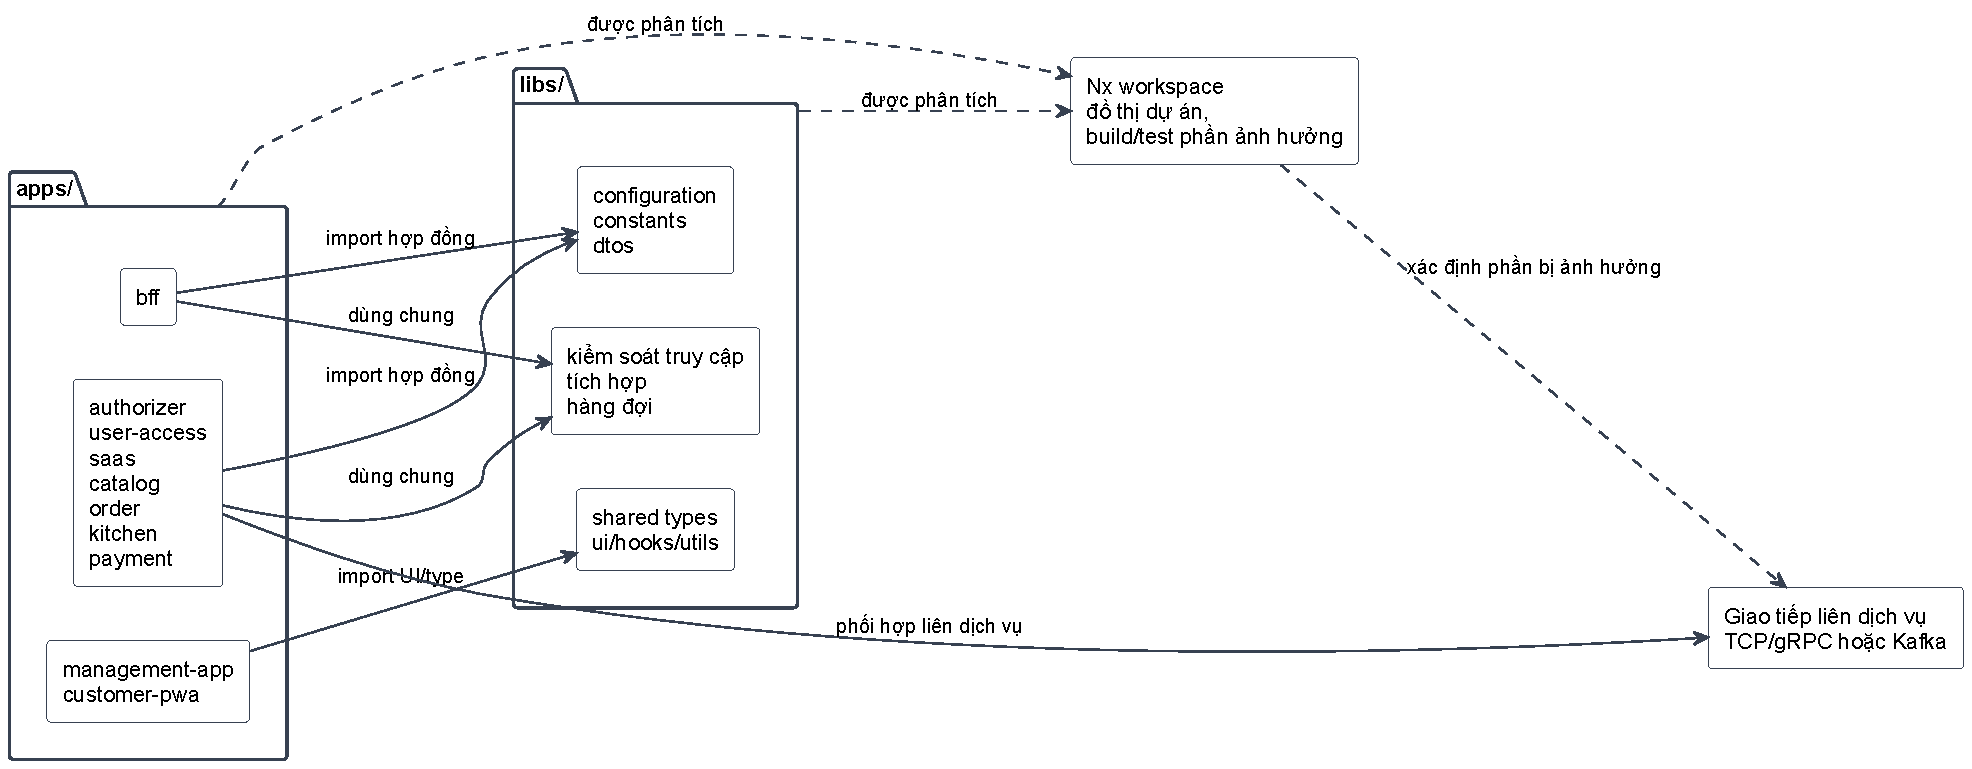
\includegraphics[width=\textwidth,height=0.82\textheight,keepaspectratio]{chapter4-nx-module-boundary.pdf}
  \caption{Ranh giới mô-đun trong Nx monorepo của QRTable.}
  \label{fig:chapter4-nx-module-boundary}
\end{figure}

\section{Ranh giới dịch vụ và trách nhiệm dữ liệu}

Bảng~\ref{tab:chapter4-service-ownership} tóm tắt trách nhiệm sở hữu chính của các thành phần trong QRTable. Đây là quyết định quan trọng nhất của Chương 4 vì nó xác định nơi đặt quy tắc nghiệp vụ, nơi lưu dữ liệu và cách các dịch vụ phối hợp mà không phá vỡ tính độc lập của từng ngữ cảnh giới hạn.

{\footnotesize
\setlength{\tabcolsep}{3pt}
\begin{longtable}{>{\raggedright\arraybackslash}p{0.15\textwidth}>{\raggedright\arraybackslash}p{0.21\textwidth}>{\raggedright\arraybackslash}p{0.28\textwidth}>{\raggedright\arraybackslash}p{0.22\textwidth}}
  \caption{Trách nhiệm dịch vụ và trách nhiệm dữ liệu chính trong QRTable.}
  \label{tab:chapter4-service-ownership}\\
  \toprule
  Thành phần & Kênh giao tiếp chính & Trách nhiệm dữ liệu & Ghi chú kiến trúc \\
  \midrule
  \endfirsthead
  \toprule
  Thành phần & Kênh giao tiếp chính & Trách nhiệm dữ liệu & Ghi chú kiến trúc \\
  \midrule
  \endhead
  \bottomrule
  \endfoot
  PWA khách & HTTP REST và WebSocket qua BFF & Không sở hữu trạng thái máy chủ & Khách dùng xác thực theo phạm vi QR/phiên, không dùng Keycloak. \\
  Ứng dụng quản trị & HTTP REST và WebSocket qua BFF & Không sở hữu trạng thái máy chủ & Gồm POS, KDS, bảng điều khiển, báo cáo và quản trị nền tảng trong một ứng dụng Next.js. \\
  BFF & HTTP REST, WebSocket, thành phần gọi TCP/gRPC & Không có CSDL nghiệp vụ riêng & Điểm vào duy nhất, chuỗi guard, định tuyến, cầu nối thời gian thực, báo cáo qua mô hình đọc và các mối quan tâm xuyên suốt. \\
  Authorizer & gRPC/TCP, API quản trị Keycloak & Không sở hữu hồ sơ ứng dụng & Xác thực JWT/OIDC cho nhân viên/chủ quán/quản trị; nguồn danh tính nằm ở Keycloak. \\
  User-Access & TCP, MongoDB/Mongoose & Hồ sơ người dùng, vai trò, ánh xạ nhân sự & Sở hữu hồ sơ ứng dụng và ánh xạ RBAC theo đơn vị thuê bao. \\
  SaaS & TCP, Kafka outbox, bộ nhớ đệm Redis & Đơn vị thuê bao, gói giá, gói thuê bao, hóa đơn gói, trạng thái quyền gói & Sở hữu vòng đời đơn vị thuê bao và trạng thái gói thuê bao; không sở hữu hồ sơ hoặc thanh toán hóa đơn nhà hàng. \\
  Catalog & TCP, dịch vụ tiêu thụ Kafka & Danh mục, món, khu vực, bàn, token QR, tồn kho & Dịch vụ duy nhất ghi tồn kho; Order chỉ gọi Catalog qua TCP khi cần trừ/hoàn tồn kho. \\
  Order & TCP, dịch vụ phát/tiêu thụ Kafka, Redis & Phiên, giỏ chung, đơn, dòng đơn, hóa đơn, yêu cầu hỗ trợ & Sở hữu vòng đời đơn/hóa đơn; không ghi trực tiếp CSDL của Catalog hoặc Payment. \\
  Kitchen & TCP, Kafka bên phát/bên tiêu thụ, Redis & Không có PostgreSQL/MongoDB riêng & Redis Sorted Set/hash là bản chiếu trạng thái khi vận hành cho hàng đợi KDS. \\
  Payment & TCP, tuyến webhook qua BFF, Kafka outbox & Thanh toán, kiểm toán thanh toán, cấu hình thanh toán của đơn vị thuê bao & Sở hữu quyết toán/cấu hình; Order vẫn sở hữu hoàn tất hóa đơn/phiên. \\
\end{longtable}
}

Catalog và Order là ví dụ điển hình cho trách nhiệm sở hữu. Khi khách gửi đơn, Order có thể lưu đơn ở trạng thái chờ xử lý và quản lý hóa đơn/phiên. Tuy nhiên, tồn kho là bất biến thuộc Catalog. Khi nhân viên xác nhận đơn, Order gọi Catalog qua TCP để trừ tồn kho trong giao dịch của Catalog. Nếu để Order ghi trực tiếp bảng món, hệ thống sẽ phá vỡ mô hình cơ sở dữ liệu riêng theo dịch vụ và khiến quy tắc xử lý tồn kho phân tán ở nhiều nơi.

Payment và Order cũng được tách tương tự. Payment sở hữu giao dịch thanh toán, cấu hình thanh toán của đơn vị thuê bao và quyết toán webhook. Order sở hữu vòng đời hóa đơn/phiên. Khi thanh toán hoàn tất, Payment có thể gọi Order theo đường nhanh có idempotency hoặc xuất bản \texttt{payment.completed} để Order xử lý phục hồi/phân phối, nhưng Payment không tự đóng hóa đơn/phiên hay cập nhật trạng thái bàn.

Kitchen là trường hợp đặc biệt vì không có PostgreSQL hoặc MongoDB riêng trong kiến trúc hiện tại. Kitchen tiêu thụ \texttt{order.confirmed}, dựng phiếu KDS và lưu hàng đợi trạng thái khi vận hành trong Redis Sorted Set/hash. Quyết định này phù hợp với yêu cầu sắp xếp FIFO, ưu tiên, SLA và cập nhật nhanh cho màn hình bếp/bar. Nếu sau này cần phân tích lịch sử bếp hoặc kiểm toán sâu hơn, có thể bổ sung lưu trữ hoặc bản chiếu riêng mà không làm thay đổi trách nhiệm của Order.

Báo cáo và bảng điều khiển trong QRTable được thiết kế theo mô hình đọc tổng hợp: BFF điều phối truy vấn, chuỗi guard kiểm soát phạm vi và quyền, còn dữ liệu nghiệp vụ vẫn do các dịch vụ sở hữu cung cấp qua hợp đồng — không tách thành dịch vụ phân tích riêng. Chủ quán và quản lý truy cập báo cáo trong phạm vi đơn vị thuê bao của mình với quyền \texttt{report.read\_own}, đồng thời chịu ràng buộc tính năng theo gói thuê bao. Quản trị nền tảng (Super Admin) dùng \texttt{report.read\_any} để phân tích xuyên đơn vị thuê bao và không bị giới hạn bởi gói của đơn vị thuê bao đang xem. Thiết kế này nằm ở lớp BFF, guard và mô hình đọc, giữ nguyên ranh giới kiến trúc lõi đã nêu.

\section{Thiết kế cơ sở dữ liệu theo ranh giới dịch vụ}

Thiết kế cơ sở dữ liệu của QRTable đi theo cùng nguyên tắc với ranh giới dịch vụ: mỗi dịch vụ sở hữu tập dữ liệu nghiệp vụ của mình, còn dịch vụ khác chỉ được truy cập thông qua hợp đồng (contract) TCP/gRPC hoặc sự kiện Kafka. Vì vậy, cơ sở dữ liệu không được xem là kho chung để các dịch vụ tùy ý nối bảng hoặc cập nhật chéo. PostgreSQL và MongoDB giữ trạng thái bền vững của từng ngữ cảnh giới hạn; Redis giữ bộ nhớ đệm, trạng thái phiên khi vận hành hoặc hàng đợi; Kafka và outbox giao dịch (transactional outbox) giữ vai trò truyền sự kiện sau điểm commit của dịch vụ phát.

\subsection{Nguyên tắc sở hữu dữ liệu}

Với các dữ liệu nằm trong phạm vi đơn vị thuê bao, \texttt{tenant\_id} là thuộc tính bắt buộc để truy vấn, khóa Redis, payload sự kiện và phòng WebSocket đều gắn với cùng ngữ cảnh. Quy tắc này không làm thay đổi việc mỗi dịch vụ vẫn có cơ sở dữ liệu hoặc nhóm dữ liệu riêng: Catalog quyết định dữ liệu catalog/tồn kho, Order quyết định phiên/đơn/hóa đơn, Payment quyết định bản ghi thanh toán và cấu hình thanh toán, SaaS quyết định đơn vị thuê bao/gói thuê bao, còn User-Access quyết định hồ sơ người dùng và vai trò nghiệp vụ. BFF và Authorizer nằm ở lớp biên/xác thực nên không được trình bày như chủ sở hữu bảng nghiệp vụ.

Bảng~\ref{tab:chapter4-data-ownership-schema} tổng hợp các bảng, collection hoặc trạng thái khi vận hành tiêu biểu theo thiết kế entity/schema của từng dịch vụ. Bảng này không thay thế ERD chi tiết; mục đích của nó là làm rõ quyền sở hữu cơ sở dữ liệu và giải thích vì sao Chương 5 mô tả luồng qua contract thay vì truy cập chéo cơ sở dữ liệu.

{\scriptsize\sloppy
\setlength{\tabcolsep}{2pt}
\begin{longtable}{>{\raggedright\arraybackslash}p{0.13\textwidth}>{\raggedright\arraybackslash}p{0.16\textwidth}>{\raggedright\arraybackslash}p{0.28\textwidth}>{\raggedright\arraybackslash}p{0.21\textwidth}>{\raggedright\arraybackslash}p{0.14\textwidth}}
  \caption{Thiết kế cơ sở dữ liệu theo ranh giới dịch vụ trong QRTable.}
  \label{tab:chapter4-data-ownership-schema}\\
  \toprule
  Dịch vụ & Kho lưu trữ chính & Bảng / collection / trạng thái tiêu biểu & Dữ liệu sở hữu & Ghi chú thiết kế \\
  \midrule
  \endfirsthead
  \toprule
  Dịch vụ & Kho lưu trữ chính & Bảng / collection / trạng thái tiêu biểu & Dữ liệu sở hữu & Ghi chú thiết kế \\
  \midrule
  \endhead
  \bottomrule
  \endfoot
  Catalog & PostgreSQL, bộ nhớ đệm Redis & \texttt{areas}, \texttt{tables}, \texttt{categories}, \texttt{menu\_items}; bộ nhớ đệm thực đơn & Khu vực, bàn, QR token, danh mục, món, khả dụng/tồn kho món & Dịch vụ duy nhất ghi dữ liệu catalog/tồn kho; Order gọi qua contract khi trừ hoặc hoàn tồn kho. \\
  Order & PostgreSQL, Redis khi vận hành & \texttt{sessions}, \texttt{orders}, \texttt{order\_items}, \texttt{bills}, \texttt{service\_requests}, \texttt{outbox\_events}; phiên/giỏ khi vận hành & Phiên gọi món, giỏ chung, đơn, dòng đơn, hóa đơn, yêu cầu phục vụ, outbox & Order sở hữu vòng đời đơn/hóa đơn; Redis hỗ trợ đường xử lý tần suất cao (hot path) cho phiên và giỏ. \\
  Kitchen & Redis & Bản chiếu phiếu, hàng đợi active/ready, revision, SLA và khóa phục hồi khi vận hành & Hàng đợi KDS theo đơn vị thuê bao và trạm bếp/bar & Không có CSDL nghiệp vụ bền vững riêng trong kiến trúc này; nhận sự kiện từ Order. \\
  Payment & PostgreSQL, trạng thái OAuth Redis & \texttt{payments}, \texttt{audit\_payments}, \texttt{tenant\_payment\_settings}, \texttt{outbox\_events}; trạng thái OAuth ngắn hạn & Giao dịch, kiểm toán thanh toán, cấu hình SePay/VietQR, outbox thanh toán & Payment sở hữu bản ghi thanh toán; Order vẫn sở hữu hoàn tất hóa đơn/phiên. \\
  SaaS & PostgreSQL, bộ nhớ đệm Redis & \texttt{tenants}, \texttt{pricing\_plans}, \texttt{subscriptions}, \texttt{subscription\_invoices}, \texttt{outbox\_events}; bộ nhớ đệm gói thuê bao & Đơn vị thuê bao, gói giá, gói thuê bao, hóa đơn gói, quyền lợi gói (entitlement) & SaaS sở hữu vòng đời đơn vị thuê bao/gói và trạng thái quyền gói. \\
  User-Access & MongoDB, tích hợp Keycloak & Collection \texttt{user}, \texttt{role} & Hồ sơ ứng dụng, vai trò nghiệp vụ, ánh xạ nhân sự theo đơn vị thuê bao & Keycloak là nguồn định danh; User-Access giữ dữ liệu nghiệp vụ về user/role. \\
  BFF / Authorizer & Không sở hữu CSDL nghiệp vụ chính & Không áp dụng & Gateway, guard, định tuyến, xác minh JWT/OIDC & Không được trình bày như dịch vụ sở hữu bảng miền nghiệp vụ. \\
\end{longtable}
}

Các sơ đồ sau đây mô tả cấu trúc dữ liệu tiêu biểu của từng dịch vụ, được trình bày bằng hình SVG xuất từ dbdiagram.io để minh họa. Sơ đồ không biểu diễn khóa ngoại (foreign key) xuyên dịch vụ vì ranh giới dữ liệu không cho phép nối CSDL trực tiếp giữa các ngữ cảnh giới hạn. Các định danh trỏ sang dịch vụ khác chỉ là tham chiếu bên ngoài (external reference) qua contract hoặc sự kiện, không phải ràng buộc CSDL chéo dịch vụ. Hình~\ref{fig:chapter4-db-catalog-schema}--\ref{fig:chapter4-db-user-access-schema} trình bày lần lượt schema tiêu biểu của Catalog, Order, Payment, SaaS và User-Access trong cùng mục thiết kế dữ liệu.

\begin{figure}[H]
  \centering
  \includesvg[width=\textwidth,height=0.82\textheight,keepaspectratio]{chapter4-db-catalog-schema.svg}
  \caption{Sơ đồ dữ liệu dịch vụ Catalog.}
  \label{fig:chapter4-db-catalog-schema}
\end{figure}

\begin{figure}[H]
  \centering
  \includesvg[width=\textwidth,height=0.82\textheight,keepaspectratio]{chapter4-db-order-schema.svg}
  \caption{Sơ đồ dữ liệu dịch vụ Order.}
  \label{fig:chapter4-db-order-schema}
\end{figure}

\begin{figure}[H]
  \centering
  \includesvg[width=\textwidth,height=0.82\textheight,keepaspectratio]{chapter4-db-payment-schema.svg}
  \caption{Sơ đồ dữ liệu dịch vụ Payment.}
  \label{fig:chapter4-db-payment-schema}
\end{figure}

\begin{figure}[H]
  \centering
  \includesvg[width=\textwidth,height=0.82\textheight,keepaspectratio]{chapter4-db-saas-schema.svg}
  \caption{Sơ đồ dữ liệu dịch vụ SaaS.}
  \label{fig:chapter4-db-saas-schema}
\end{figure}

\begin{figure}[H]
  \centering
  \includesvg[width=\textwidth,height=0.82\textheight,keepaspectratio]{chapter4-db-user-access-schema.svg}
  \caption{Sơ đồ dữ liệu dịch vụ User-Access (mô hình tài liệu MongoDB, mô phỏng bằng DBML).}
  \label{fig:chapter4-db-user-access-schema}
\end{figure}

\subsection{Ý nghĩa đối với các dịch vụ nghiệp vụ}

Ở nhóm Catalog--Order, bảng dữ liệu phản ánh trực tiếp điểm commit nghiệp vụ. Catalog lưu bàn, khu vực, danh mục và món; vì vậy tồn kho và khả dụng món thuộc về Catalog. Order lưu phiên, giỏ, đơn, dòng đơn và hóa đơn; vì vậy Order có thể quyết định đơn đang ở trạng thái nào, nhưng không tự sửa bảng món của Catalog. Luồng xác nhận đơn ở Chương 5 vì thế phải đi qua lời gọi Order--Catalog, có idempotency và bù trừ, thay vì tạo một giao dịch cơ sở dữ liệu dùng chung.

Ở nhóm Kitchen, Redis chỉ là bản chiếu trạng thái khi vận hành của dữ liệu đã được commit ở Order. Kitchen dựng phiếu KDS từ \texttt{order.confirmed}, lưu hàng đợi theo trạm, phát gợi ý WebSocket và cho phép client lấy lại snapshot. Nếu cần truy xuất lịch sử đơn, hệ thống quay về Order hoặc các nguồn bền vững khác; hàng đợi KDS không được xem như nguồn dữ liệu lịch sử có thẩm quyền.

Ở nhóm Payment--SaaS--User-Access, ranh giới dữ liệu giúp tách hai dòng tiền và hai loại danh tính. Payment lưu bản ghi thanh toán và cấu hình SePay/VietQR cho hóa đơn nhà hàng; SaaS lưu đơn vị thuê bao, gói giá, subscription và hóa đơn gói nền tảng; User-Access lưu hồ sơ ứng dụng và vai trò nghiệp vụ trong MongoDB trong khi Keycloak giữ định danh. Cách tách này giúp webhook, khởi tạo đơn vị thuê bao (onboarding) và quyền lợi gói (entitlement) được giải thích theo chủ sở hữu rõ ràng, không gom vào một bảng người dùng hoặc thanh toán chung.

Tóm lại, thiết kế dữ liệu theo dịch vụ là bằng chứng cụ thể cho ranh giới dịch vụ (service boundary) của QRTable. Khi Chương 5 trình bày các luồng phiên QR, xác nhận đơn, KDS, thanh toán và onboarding, mỗi luồng đều phải đi qua contract giữa dịch vụ thay vì nối bảng hoặc cập nhật chéo cơ sở dữ liệu. Đây là điểm quan trọng để hệ thống giữ được tính độc lập theo ngữ cảnh giới hạn trong một Nx monorepo.

\section{Chiến lược đa đơn vị thuê bao}

Hình~\ref{fig:chapter4-multi-tenancy-isolation} minh họa cách ngữ cảnh đơn vị thuê bao đi qua API, dịch vụ, cơ sở dữ liệu, Redis, Kafka và WebSocket. Mô hình hiện tại là cơ sở dữ liệu riêng theo dịch vụ kết hợp cột phân biệt \texttt{tenant\_id}. Với các bảng thuộc phạm vi nhà hàng như món, bàn, đơn, hóa đơn, thanh toán hoặc gói thuê bao, \texttt{tenant\_id} là điều kiện bắt buộc để tách dữ liệu giữa các đơn vị thuê bao.

\begin{figure}[H]
  \centering
  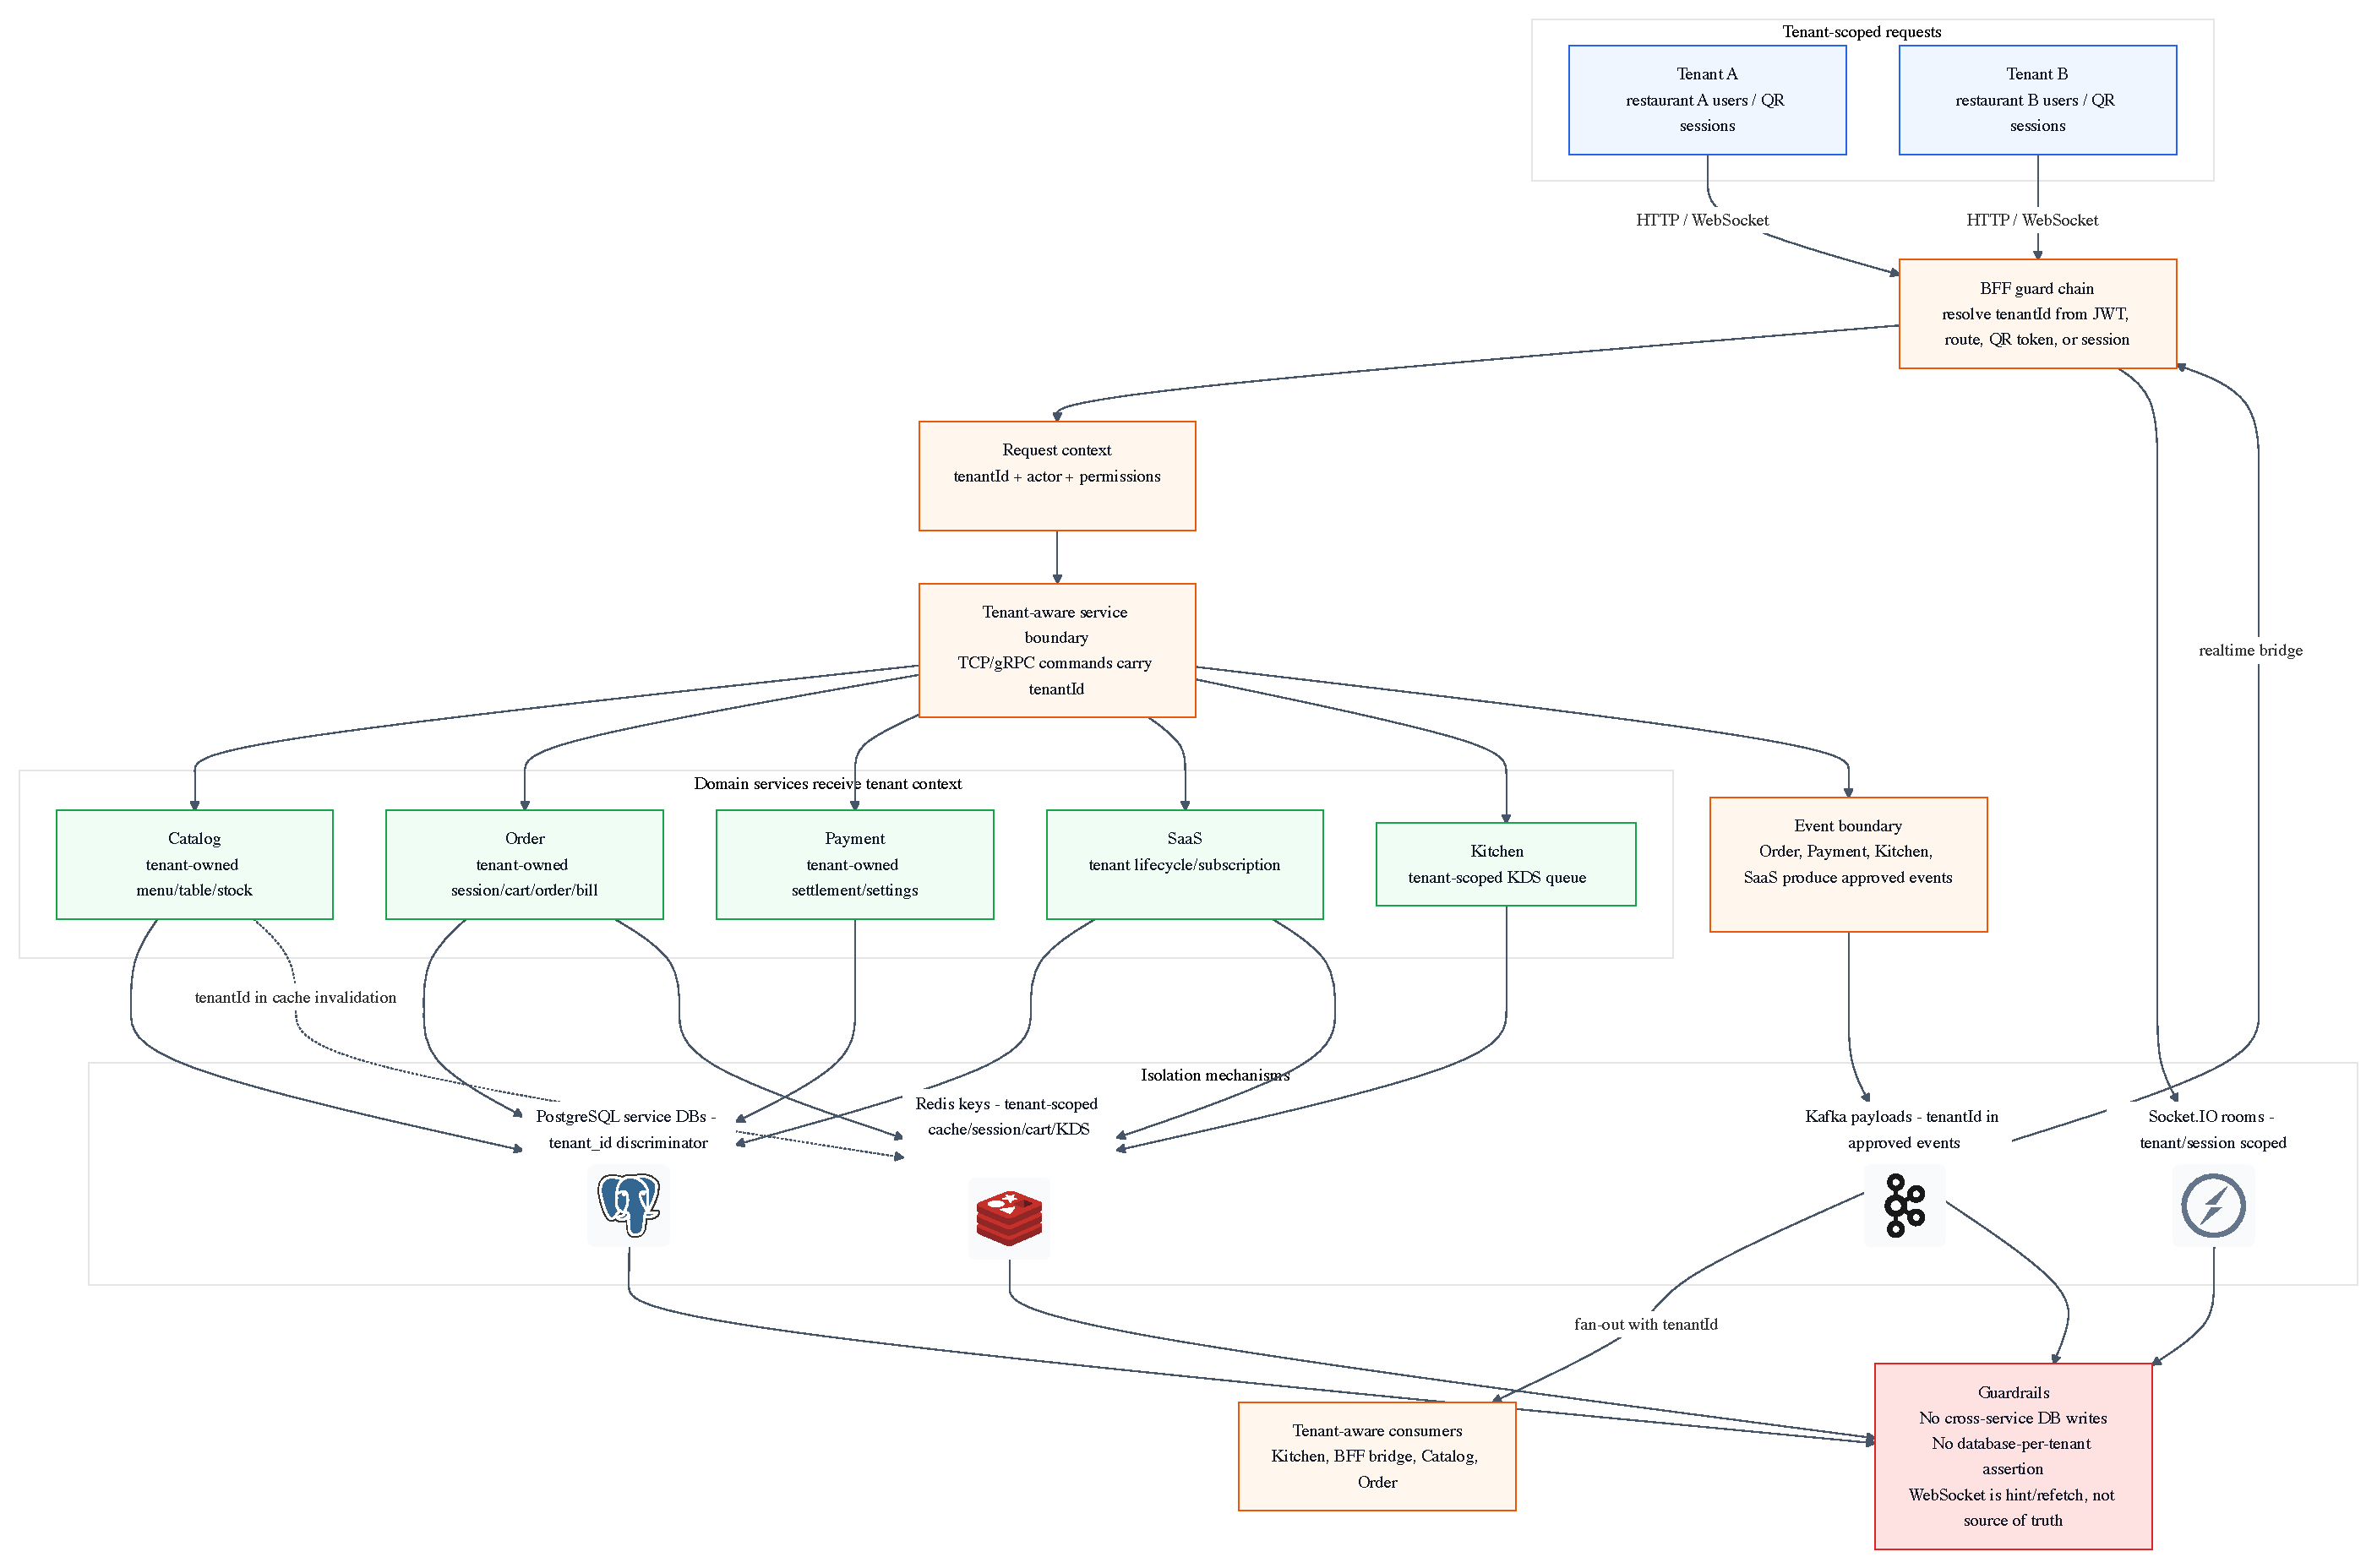
\includegraphics[width=\textwidth]{chapter4-multi-tenancy-isolation.pdf}
  \caption{Cơ chế cô lập đơn vị thuê bao ở API, dịch vụ, cơ sở dữ liệu, Redis, Kafka và WebSocket.}
  \label{fig:chapter4-multi-tenancy-isolation}
\end{figure}

Ở lớp yêu cầu, nhân viên/chủ quán/quản trị đi qua JWT/OIDC và khẳng định đơn vị thuê bao, còn khách đi qua ngữ cảnh theo phạm vi QR/phiên. BFF và chuỗi guard có trách nhiệm đưa ngữ cảnh đơn vị thuê bao vào yêu cầu trước khi gọi dịch vụ. Ở lớp dịch vụ, repository/truy vấn phải lọc theo đơn vị thuê bao. Ở lớp bộ nhớ đệm, khóa Redis dùng không gian tên theo đơn vị thuê bao cho thực đơn, phiên, giỏ và hàng đợi KDS. Ở lớp sự kiện, payload Kafka phải có \texttt{tenantId} để bên tiêu thụ (Consumer) định tuyến và xử lý đúng đơn vị thuê bao. Ở lớp thời gian thực, phòng WebSocket dùng không gian tên đơn vị thuê bao/phiên để tránh phát sự kiện sang sai nhóm người dùng.

Đánh đổi của mô hình này là QRTable chưa đạt mức cô lập vật lý như một cơ sở dữ liệu riêng cho mỗi đơn vị thuê bao. Nếu hệ thống đi tới quy mô lớn hơn hoặc có yêu cầu tuân thủ cao hơn, có thể cân nhắc lược đồ riêng cho mỗi đơn vị thuê bao, cơ sở dữ liệu riêng cho mỗi đơn vị thuê bao hoặc mô hình lai. Tuy nhiên, đối với mục tiêu khóa luận và giai đoạn xây dựng hiện tại, cơ sở dữ liệu riêng theo dịch vụ kết hợp \texttt{tenant\_id} tạo được cân bằng giữa trách nhiệm sở hữu, chi phí vận hành và khả năng kiểm thử bằng dữ liệu minh họa.

\section{Kiến trúc giao tiếp giữa các dịch vụ}

Bảng~\ref{tab:chapter4-communication-matrix} trình bày các kênh giao tiếp chính trong QRTable. Hệ thống không áp dụng một cơ chế duy nhất cho mọi tương tác. Mỗi kênh được chọn theo yêu cầu phản hồi, mức phụ thuộc, tính bất đồng bộ và trách nhiệm của thao tác nghiệp vụ.

{\footnotesize
\setlength{\tabcolsep}{3pt}
\begin{longtable}{>{\raggedright\arraybackslash}p{0.16\textwidth}>{\raggedright\arraybackslash}p{0.24\textwidth}>{\raggedright\arraybackslash}p{0.28\textwidth}>{\raggedright\arraybackslash}p{0.18\textwidth}}
  \caption{Ma trận giao tiếp của QRTable.}
  \label{tab:chapter4-communication-matrix}\\
  \toprule
  Kênh & Từ--Đến & Mục đích & Ranh giới kiểm soát \\
  \midrule
  \endfirsthead
  \toprule
  Kênh & Từ--Đến & Mục đích & Ranh giới kiểm soát \\
  \midrule
  \endhead
  \bottomrule
  \endfoot
  HTTP REST & PWA khách / ứng dụng quản trị -- BFF & API bên ngoài, xác thực tuyến, kiểm tra đầu vào và điều phối yêu cầu ở lớp biên. & Phía người dùng không gọi dịch vụ nội bộ trực tiếp. \\
  WebSocket / Socket.IO & BFF -- khách / nhân viên / KDS / quản trị & Gợi ý thời gian thực, làm mất hiệu lực và làm mới dữ liệu cho đơn, giỏ, KDS, thanh toán và vòng đời đơn vị thuê bao. & Không phải trạng thái có thẩm quyền. \\
  TCP RPC & BFF -- Catalog / Order / Kitchen / Payment / SaaS / User-Access & Lệnh/truy vấn nội bộ cần phản hồi ngay. & Không dùng thay cho phân phối sự kiện. \\
  TCP RPC & Order -- Catalog & Trừ/hoàn tồn kho và thao tác bàn theo trách nhiệm của Catalog. & Order không ghi CSDL Catalog. \\
  TCP RPC & Payment -- Order & Lấy snapshot hóa đơn và đánh dấu đã thanh toán theo cách có idempotency cho đường nhanh/phục hồi. & Payment không sở hữu hóa đơn/phiên. \\
  TCP RPC & SaaS -- Authorizer / User-Access / Payment / Catalog / Order & Mini-saga đưa đơn vị thuê bao vào hệ thống, tạo chủ quán/hồ sơ/cấu hình, bộ đếm sử dụng và hạn mức. & Điều phối SaaS không đồng nghĩa sở hữu dữ liệu của dịch vụ khác. \\
  gRPC & BFF -- Authorizer & Xác minh token và đường xác thực nhanh bằng contract dịch vụ có kiểu. & Luồng QR khách không đi qua Keycloak. \\
  Kafka & Order / Payment / Kitchen / SaaS -- bên tiêu thụ & Sự kiện miền bất đồng bộ, tách thời gian, phân phối và phục hồi. & Chỉ dùng 5 topic được chấp nhận. \\
  Gợi ý nội bộ Redis & Trạng thái KDS khi vận hành -- cầu nối WebSocket BFF & Báo hàng đợi KDS thay đổi sau khi ghi Redis. & Gợi ý/làm mới, không thay trạng thái Kitchen. \\
  Webhook HTTP & SePay -- BFF -- Payment/SaaS & Quyết toán chuyển khoản cho hóa đơn nhà hàng \texttt{QRTBL} và hóa đơn gói \texttt{QRSUB}. & Không trộn tuyến webhook theo tầng. \\
  HTTP/API ngoài & Catalog / Payment / Authorizer -- Cloudinary / SePay / Keycloak & Tải ảnh, API OAuth/nhà cung cấp và thao tác quản trị IAM. & Chỉ khẳng định phần có mã/bằng chứng. \\
\end{longtable}
}

Hình~\ref{fig:chapter4-communication-topology} đặt các kênh trong Bảng~\ref{tab:chapter4-communication-matrix} vào cùng một bản đồ. Phía người dùng chỉ giao tiếp với BFF bằng HTTP REST hoặc WebSocket; BFF gọi dịch vụ nội bộ bằng TCP/gRPC khi cần phản hồi ngay; Kafka chỉ nhận các sự kiện miền đã được chấp nhận; Redis hỗ trợ gợi ý/làm mới hoặc trạng thái chạy; webhook từ SePay đi qua BFF trước khi được định tuyến đến Payment hoặc SaaS.

\begin{figure}[H]
  \centering
  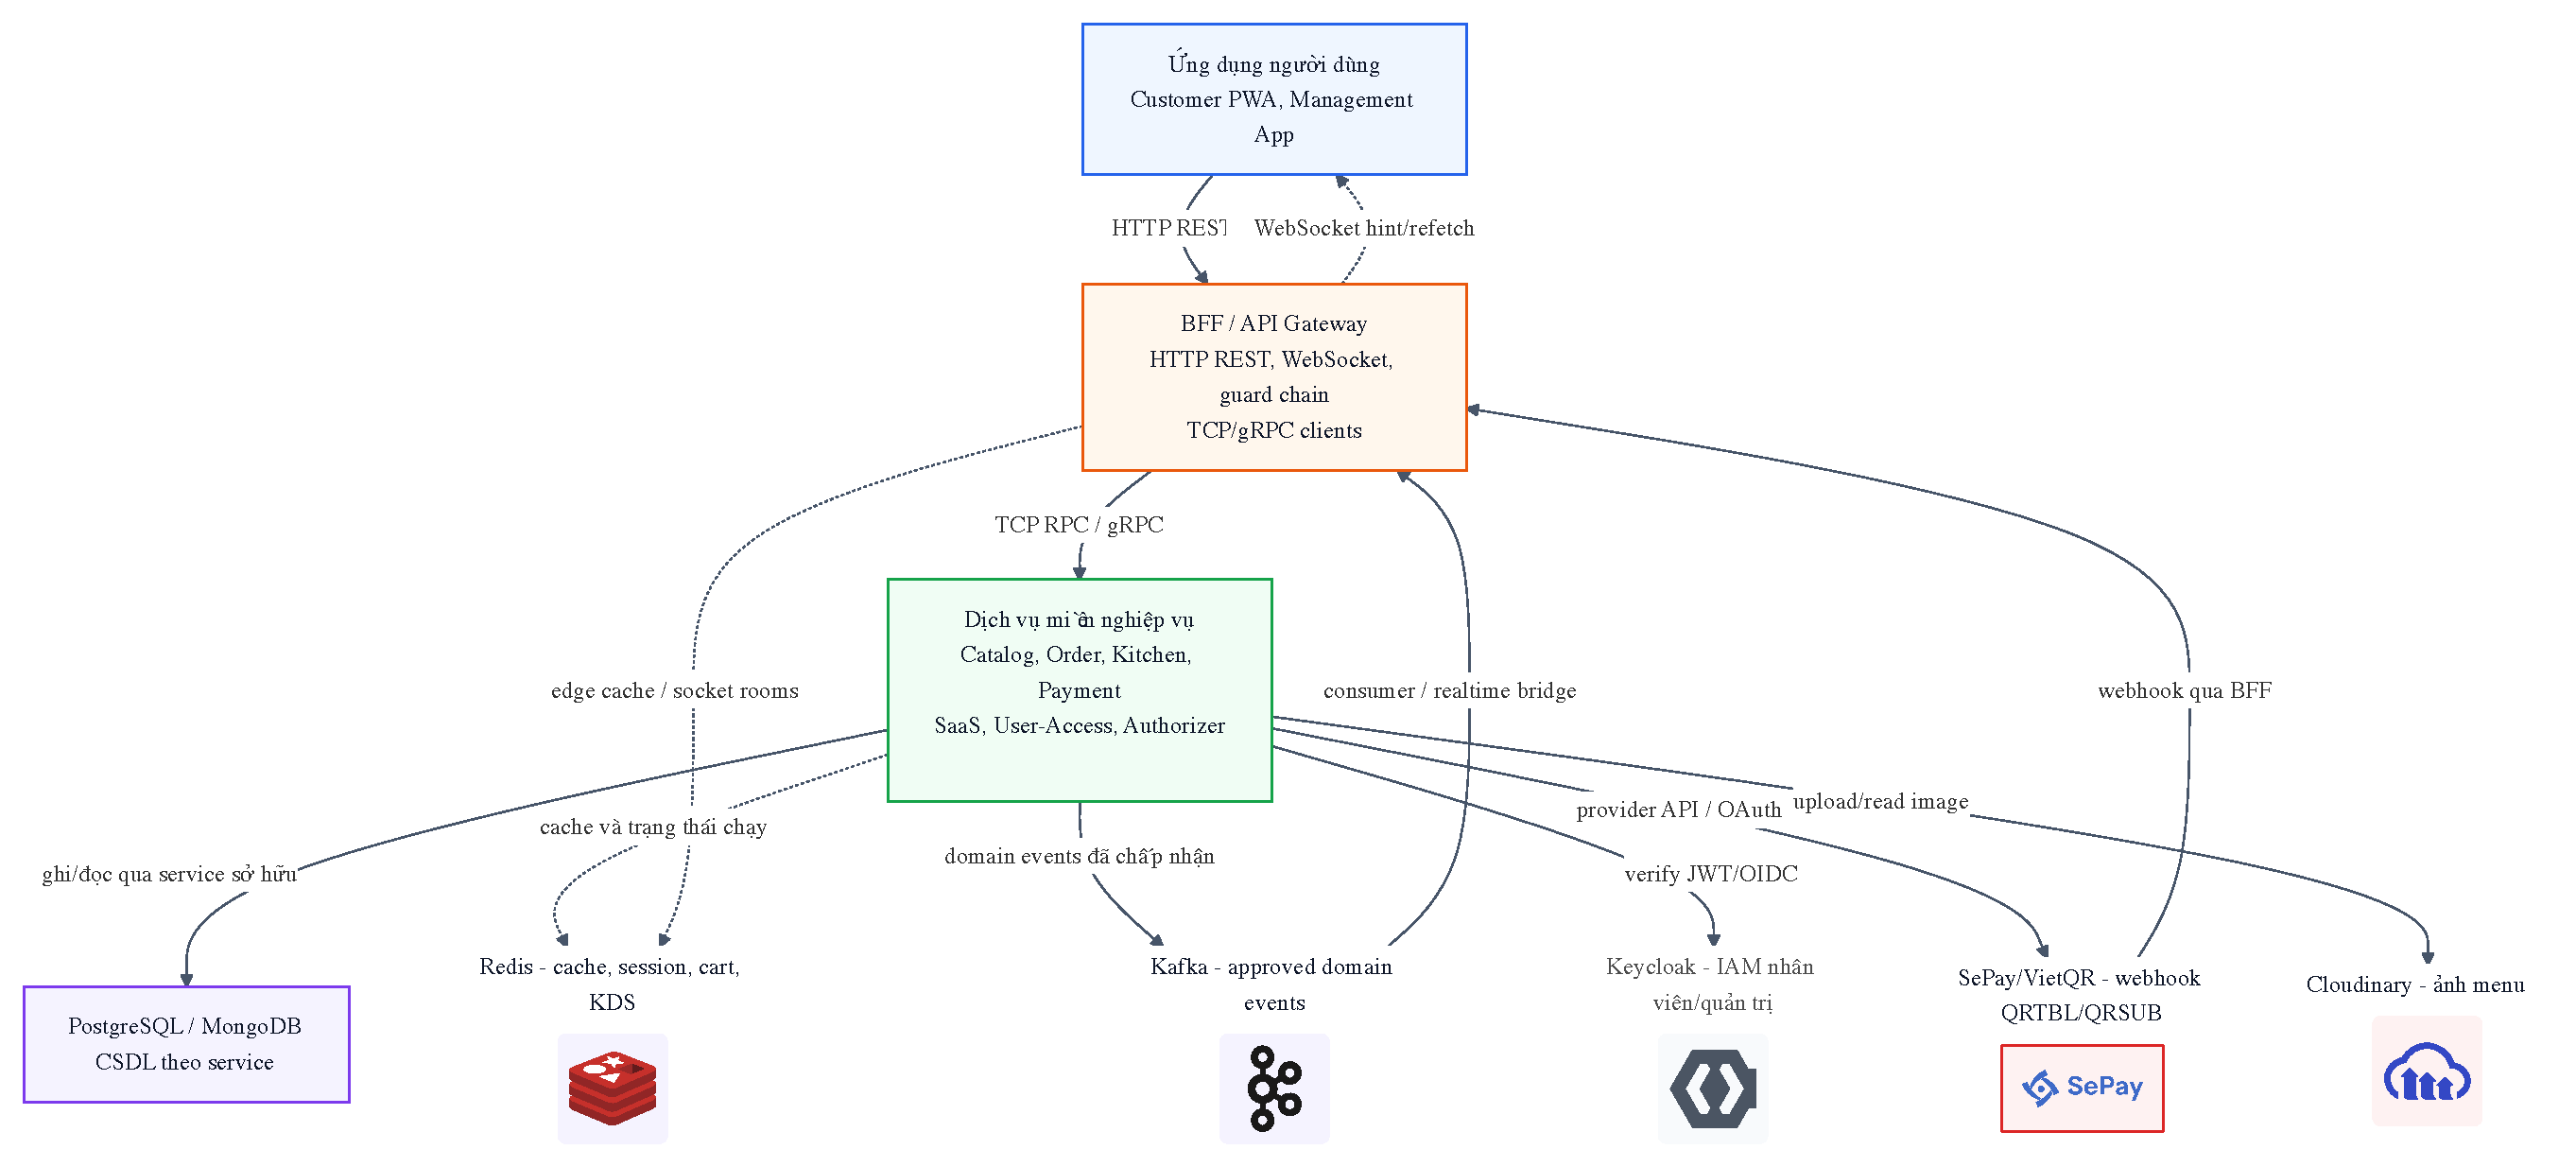
\includegraphics[width=\textwidth,height=0.82\textheight,keepaspectratio]{chapter4-communication-topology.pdf}
  \caption{Bản đồ giao tiếp giữa các thành phần QRTable.}
  \label{fig:chapter4-communication-topology}
\end{figure}

HTTP REST chỉ xuất hiện ở ranh giới ứng dụng đến BFF hoặc nhà cung cấp ngoài đến BFF. TCP RPC được dùng cho lệnh/truy vấn nội bộ cần kết quả ngay, ví dụ BFF cần trả phản hồi thực đơn/đơn cho phía client, Order cần biết Catalog có trừ tồn kho thành công hay không, hoặc Payment cần lấy snapshot hóa đơn từ Order. gRPC được dùng cho đường xác thực đến Authorizer vì đây là đường nhanh có contract có kiểu.

Kafka được dùng khi bên phát (Producer) không cần đợi bên tiêu thụ (Consumer) hoàn thành hoặc khi sự kiện cần kích hoạt phản ứng nghiệp vụ ở ngữ cảnh giới hạn khác. Ví dụ, khi đơn được xác nhận, Order không cần chờ Kitchen tạo xong phiếu KDS để trả kết quả xác nhận cho nhân viên; do đó \texttt{order.confirmed} đi qua Kafka. Ngược lại, khi khách cập nhật giỏ hoặc khi BFF cần phát thông báo cho client sau một phản hồi TCP đã thành công, dùng Kafka sẽ làm tăng độ trễ và phụ thuộc hạ tầng mà không thêm giá trị nghiệp vụ. Trường hợp này được xử lý bằng đường trực tiếp qua BFF hoặc gợi ý WebSocket/làm mới dữ liệu.

WebSocket trong QRTable được dùng để cải thiện trải nghiệm thời gian thực nhưng không thay thế nguồn sự thật của hệ thống. Theo bản chất giao thức, WebSocket cung cấp kênh hai chiều lâu dài giữa phía người dùng và máy chủ \cite{fette-websocket-rfc6455-2011}; trong QRTable, kênh này chỉ mang sự kiện thông báo, làm mất hiệu lực hoặc gợi ý làm mới. Nếu phía người dùng mất kết nối hoặc nhận sự kiện trễ, trạng thái đúng vẫn phải được lấy lại từ API và dịch vụ sở hữu.

\section{Thiết kế hướng sự kiện và sổ đăng ký topic Kafka}

Hình~\ref{fig:chapter4-kafka-decision-flow} trình bày luồng quyết định chọn TCP/gRPC, Kafka, WebSocket/đường trực tiếp qua BFF hoặc bộ chuyển đổi webhook. Luồng này giúp tránh hai cực đoan: dùng Kafka cho mọi thứ, hoặc dùng RPC đồng bộ cho các tác dụng phụ có thể chạy bất đồng bộ.

\begin{figure}[H]
  \centering
  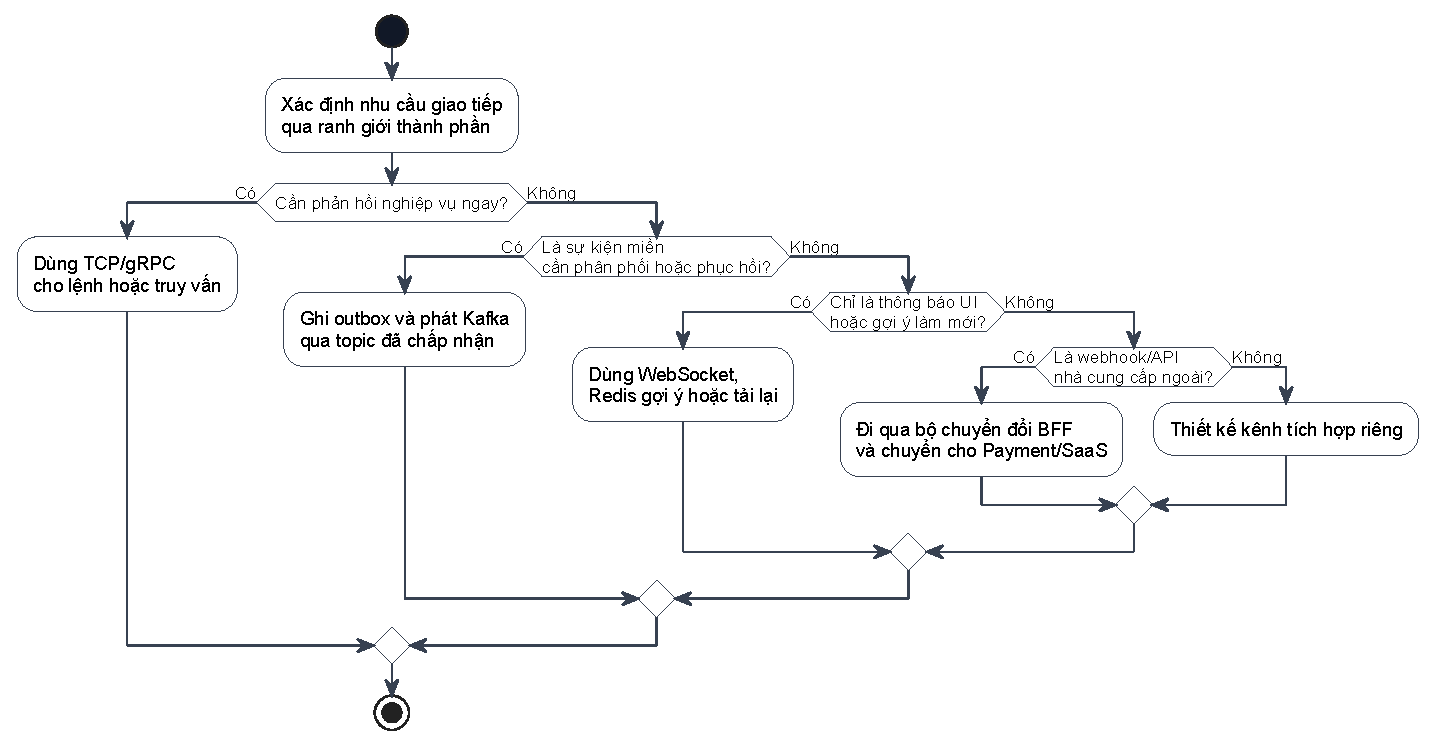
\includegraphics[width=\textwidth,height=0.82\textheight,keepaspectratio]{chapter4-kafka-decision-flow.pdf}
  \caption{Luồng quyết định chọn TCP/gRPC, Kafka, WebSocket/đường trực tiếp qua BFF hoặc bộ chuyển đổi webhook.}
  \label{fig:chapter4-kafka-decision-flow}
\end{figure}

\subsection{Vai trò của Kafka trong kiến trúc QRTable}

Khung quyết định của QRTable có thể tóm tắt như sau. Nếu một thay đổi trạng thái cần quy tắc nghiệp vụ ở ngữ cảnh giới hạn khác, Kafka là lựa chọn phù hợp. Nếu bên phát không cần đợi bên tiêu thụ, hoặc sự kiện được tạo bởi bộ hẹn giờ/tiến trình nền nội bộ, Kafka cũng phù hợp. Nếu sự kiện là kết quả của một ghi CSDL và cần phát ra ngoài dịch vụ, outbox giao dịch (transactional outbox) được dùng để giảm rủi ro ghi kép. Ngược lại, nếu tác dụng phụ chỉ là thông báo cho client hoặc làm mất hiệu lực bộ nhớ đệm sau khi BFF đã có phản hồi từ TCP, đường trực tiếp qua BFF là lựa chọn đơn giản hơn.

Do đó, Kafka trong QRTable không phải lớp trung gian cho mọi lời gọi. Lệnh hoặc truy vấn cần phản hồi ngay vẫn đi qua TCP/gRPC, ví dụ Order gọi Catalog để trừ tồn kho khi nhân viên xác nhận đơn, BFF gọi Order để lấy trạng thái phiên hoặc Payment gọi Order để lấy snapshot hóa đơn. Kafka chỉ xuất hiện khi sự kiện đã xảy ra ở một dịch vụ sở hữu và cần kích hoạt phản ứng bất đồng bộ ở dịch vụ khác, như Kitchen dựng phiếu KDS từ \texttt{order.confirmed}, Order hoàn tất hóa đơn từ \texttt{payment.completed}, Catalog tạo dữ liệu mặc định từ \texttt{tenant.created}, hoặc BFF phát cảnh báo thời gian thực từ \texttt{kitchen.sla\_warning}.

\subsection{Sổ đăng ký topic và hợp đồng sự kiện}

Bảng~\ref{tab:chapter4-kafka-topic-registry} liệt kê năm topic được chấp nhận trong sổ đăng ký hiện tại. Mỗi dòng trình bày topic như một hợp đồng (contract) kiến trúc: bên phát, bên tiêu thụ, khóa phân vùng, payload chính và cơ chế độ tin cậy/idempotency theo quyết định thiết kế. Payload trong bảng chỉ nêu các trường đại diện để người đọc hiểu ý nghĩa sự kiện, không thay thế định nghĩa DTO đầy đủ trong triển khai.

{\scriptsize
\setlength{\tabcolsep}{1pt}
\begin{longtable}{>{\raggedright\arraybackslash}p{0.12\textwidth}>{\raggedright\arraybackslash}p{0.08\textwidth}>{\raggedright\arraybackslash}p{0.13\textwidth}>{\raggedright\arraybackslash}p{0.08\textwidth}>{\raggedright\arraybackslash}p{0.18\textwidth}>{\raggedright\arraybackslash}p{0.13\textwidth}>{\raggedright\arraybackslash}p{0.14\textwidth}}
  \caption{Hợp đồng sự kiện Kafka được chấp nhận trong QRTable.}
  \label{tab:chapter4-kafka-topic-registry}\\
  \toprule
  Topic & Bên phát & Bên tiêu thụ / trạng thái & Khóa phân vùng & Payload chính & Lý do dùng Kafka & Độ tin cậy / idempotency \\
  \midrule
  \endfirsthead
  \toprule
  Topic & Bên phát & Bên tiêu thụ / trạng thái & Khóa phân vùng & Payload chính & Lý do dùng Kafka & Độ tin cậy / idempotency \\
  \midrule
  \endhead
  \bottomrule
  \endfoot
  \texttt{order.}\newline\texttt{confirmed} & Order & Kitchen & \texttt{tenantId} & \texttt{eventId}, \texttt{tenantId}, \texttt{orderId}, \texttt{sessionId}, \texttt{tableId}, \texttt{items[]}, \texttt{confirmedAt}, \texttt{confirmedByUserId} & Đơn đã xác nhận cần tạo phiếu KDS nhưng Order không cần đợi Kitchen xử lý xong. & Outbox Order; Kitchen khử trùng theo \texttt{eventId} và cặp đơn/trạm. \\
  \texttt{order.}\newline\texttt{status\_}\newline\texttt{changed} & Order & Bản chiếu / kiểm toán khi có bên tiêu thụ phù hợp & \texttt{tenantId} & \texttt{tenantId}, \texttt{orderId}, \texttt{fromStatus}, \texttt{toStatus}, \texttt{timestamp} & Dòng trạng thái bền vững cho bản chiếu hoặc kiểm toán; phản hồi client tức thời vẫn đi qua BFF. & Outbox Order; bên tiêu thụ phải xử lý bản ghi trùng theo aggregate và trạng thái đích. \\
  \texttt{payment.}\newline\texttt{completed} & Payment & Order, cầu nối thời gian thực BFF & \texttt{tenantId} & \texttt{eventId}, \texttt{tenantId}, \texttt{billId}, \texttt{paymentId}, \texttt{method}, \texttt{amount}, \texttt{paidAt} & Thanh toán hoàn tất cần chốt hóa đơn, đồng thời phát gợi ý thời gian thực cho khách và nhân viên. & Outbox Payment; Order đánh dấu hóa đơn đã thanh toán theo hướng idempotency. \\
  \texttt{kitchen.sla\_}\newline\texttt{warning} & Kitchen & Cầu nối thời gian thực BFF & \texttt{tenantId} & \texttt{eventId}, \texttt{tenantId}, \texttt{ticketId}, \texttt{station}, \texttt{level}, \texttt{waitTimeSeconds}, \texttt{thresholdSeconds} & Cảnh báo SLA là sự kiện hẹn giờ/nội bộ, không gắn với yêu cầu TCP đang chờ phản hồi. & Tiến trình SLA dùng nhóm khử trùng; BFF chỉ phát cảnh báo, không sở hữu trạng thái KDS. \\
  \texttt{tenant.}\newline\texttt{created} & SaaS & Catalog & \texttt{tenantId} & \texttt{eventId}, \texttt{tenantId}, \texttt{slug}, \texttt{name}, thông tin chủ sở hữu, \texttt{planCode}, \texttt{correlationId} & Khởi tạo đơn vị thuê bao cần khởi tạo dữ liệu mặc định ở Catalog mà không siết phụ thuộc trong quy trình onboarding. & Outbox SaaS; bên tiêu thụ Catalog kiểm tra dữ liệu mặc định trước khi tạo. \\
\end{longtable}
}

\subsection{Outbox giao dịch và kỷ luật phát sự kiện}

Các sự kiện phát sinh từ ghi CSDL không được gửi thẳng ra Kafka như một thao tác rời rạc. QRTable dùng outbox giao dịch (transactional outbox): trong cùng giao dịch nghiệp vụ, dịch vụ ghi dữ liệu miền và ghi thêm một dòng \texttt{outbox\_events}. Tiến trình xuất bản sau đó đọc các dòng \texttt{PENDING}, gửi Kafka với \texttt{key = partition\_key}, rồi đánh dấu \texttt{PUBLISHED}; nếu lỗi, dòng được tăng số lần thử và giữ trạng thái có thể retry hoặc chuyển \texttt{FAILED} sau ngưỡng lỗi. Thiết kế này giảm rủi ro ghi dữ liệu thành công nhưng mất sự kiện, nhưng không được diễn đạt như CDC, Debezium hoặc bảo đảm phân phối exactly-once.

{\footnotesize
\setlength{\tabcolsep}{3pt}
\begin{longtable}{>{\raggedright\arraybackslash}p{0.2\textwidth}>{\raggedright\arraybackslash}p{0.36\textwidth}>{\raggedright\arraybackslash}p{0.36\textwidth}}
  \caption{Các trường outbox và kỷ luật phát sự kiện trong QRTable.}
  \label{tab:chapter4-outbox-discipline}\\
  \toprule
  Trường outbox & Ý nghĩa thiết kế & Tác dụng trong QRTable \\
  \midrule
  \endfirsthead
  \toprule
  Trường outbox & Ý nghĩa thiết kế & Tác dụng trong QRTable \\
  \midrule
  \endhead
  \bottomrule
  \endfoot
  \texttt{tenant\_id} & Giữ ngữ cảnh đơn vị thuê bao của dòng sự kiện. & Tiến trình xuất bản cập nhật đúng dòng theo đơn vị thuê bao; bên tiêu thụ định tuyến xử lý trong phạm vi đơn vị thuê bao. \\
  \texttt{topic} & Đích Kafka cần phát. & Ràng buộc sự kiện với sổ đăng ký topic đã chấp nhận. \\
  \texttt{event\_type} & Tên sự kiện theo nghĩa nghiệp vụ. & Bên tiêu thụ kiểm tra đúng loại sự kiện trước khi áp dụng tác dụng phụ. \\
  \texttt{aggregate\_id} & Định danh aggregate phát sinh sự kiện. & Hỗ trợ kiểm toán, idempotency và truy vết từ sự kiện về đơn/thanh toán/đơn vị thuê bao. \\
  \texttt{partition\_key} & Khóa thông điệp khi gửi Kafka. & Hiện dùng \texttt{tenantId} để gom thứ tự xử lý theo đơn vị thuê bao ở mức hợp lý. \\
  \texttt{payload} & Nội dung JSONB được ghi sau khi commit nghiệp vụ. & Lưu lại nội dung sự kiện để tiến trình xuất bản có thể retry mà không cần tính lại từ nhiều bảng. \\
  \texttt{status} & Trạng thái \texttt{PENDING}, \texttt{PUBLISHED} hoặc \texttt{FAILED}. & Tách rõ dòng cần gửi, đã gửi và gửi lỗi vượt ngưỡng. \\
  \texttt{attempt\_count}, \texttt{last\_error} & Theo dõi số lần retry và lỗi gần nhất. & Hỗ trợ retry có kiểm soát và điều tra lỗi xuất bản. \\
  \texttt{published\_at} & Thời điểm phát thành công. & Cho phép đối chiếu độ trễ xuất bản và trạng thái dòng outbox khi kiểm chứng. \\
\end{longtable}
}

\subsection{Ranh giới giữa Kafka, đường trực tiếp qua BFF và WebSocket}

Bảng~\ref{tab:chapter4-kafka-topic-registry} cũng thể hiện một ranh giới kiểm soát quan trọng: QRTable chỉ công nhận năm topic trong sổ đăng ký hiện tại. Các sự kiện như giỏ cập nhật, yêu cầu hóa đơn, chuyển bàn, hàng đợi KDS thay đổi, đơn vị thuê bao bị tạm ngưng hoặc thực đơn cập nhật không được viết như topic Kafka lõi nếu chưa có hợp đồng tương ứng. Chúng có thể là sự kiện socket, gợi ý nội bộ Redis, làm mất hiệu lực bộ nhớ đệm hoặc làm mới client tùy trường hợp.

Đường thời gian thực của BFF vì vậy có hai nguồn khác nhau. Với hai topic thanh toán và cảnh báo SLA đã được phê duyệt, BFF có thể tiêu thụ Kafka để phát WebSocket. Với hàng đợi KDS thay đổi sau thao tác bếp hoặc sau khi Kitchen ghi Redis, Kitchen phát \texttt{kds.queue\_changed} vào Redis Pub/Sub theo mẫu \texttt{realtime:kds:*}; BFF đăng ký nhận kênh này và phát tới phòng KDS bếp/bar tương ứng. Sự kiện đó là gợi ý làm mới client, không phải topic Kafka và không phải nguồn trạng thái bếp có thẩm quyền.

\subsection{Giới hạn thiết kế và các khẳng định không mở rộng}

Kafka trong QRTable được thiết kế theo hướng ít nhất một lần (at-least-once) ở mức thực tế triển khai: bên phát có thể retry, tiến trình outbox có thể gửi lại dòng chưa đánh dấu thành công và bên tiêu thụ phải xử lý bản ghi trùng bằng \texttt{eventId}, \texttt{aggregate\_id} hoặc khóa idempotency riêng. Khóa luận vì vậy không khẳng định phân phối exactly-once, không khẳng định CDC/Debezium và không dùng Kafka để chứng minh mọi tính nhất quán dữ liệu (consistency). Tính đúng của tồn kho vẫn nằm ở Catalog và giao dịch xác nhận đơn; tính đúng của hóa đơn vẫn nằm ở Order/Payment; Kafka chỉ giúp tách thời gian và phục hồi tác dụng phụ sau điểm commit.

\section{Redis cho bộ nhớ đệm, trạng thái khi vận hành và KDS}

\subsection{Nguyên tắc sở hữu Redis theo miền nghiệp vụ}

Redis được dùng vì một số trạng thái có tần suất đọc/ghi cao, cần TTL hoặc cần cấu trúc dữ liệu khi vận hành phù hợp hơn cơ sở dữ liệu quan hệ. Tuy nhiên, mỗi nhóm khóa phải có dịch vụ sở hữu rõ ràng. QRTable không dùng Redis như một cơ sở dữ liệu nghiệp vụ chia sẻ giữa các dịch vụ; Redis chỉ giữ bộ nhớ đệm, trạng thái khi vận hành, cờ ngắn hạn, khóa idempotency hoặc bản chiếu phục vụ thời gian thực.

Hình~\ref{fig:chapter4-redis-ownership} tách Redis theo nhóm khóa và dịch vụ sở hữu. Cách trình bày này giúp tránh hiểu nhầm Redis là kho trạng thái chung của toàn hệ thống. Với mỗi nhóm khóa, Redis chỉ giữ bộ nhớ đệm, cờ vận hành ngắn hạn hoặc bản chiếu khi vận hành; nguồn sự thật (source of truth) vẫn nằm ở dịch vụ sở hữu.

\begin{figure}[H]
  \centering
  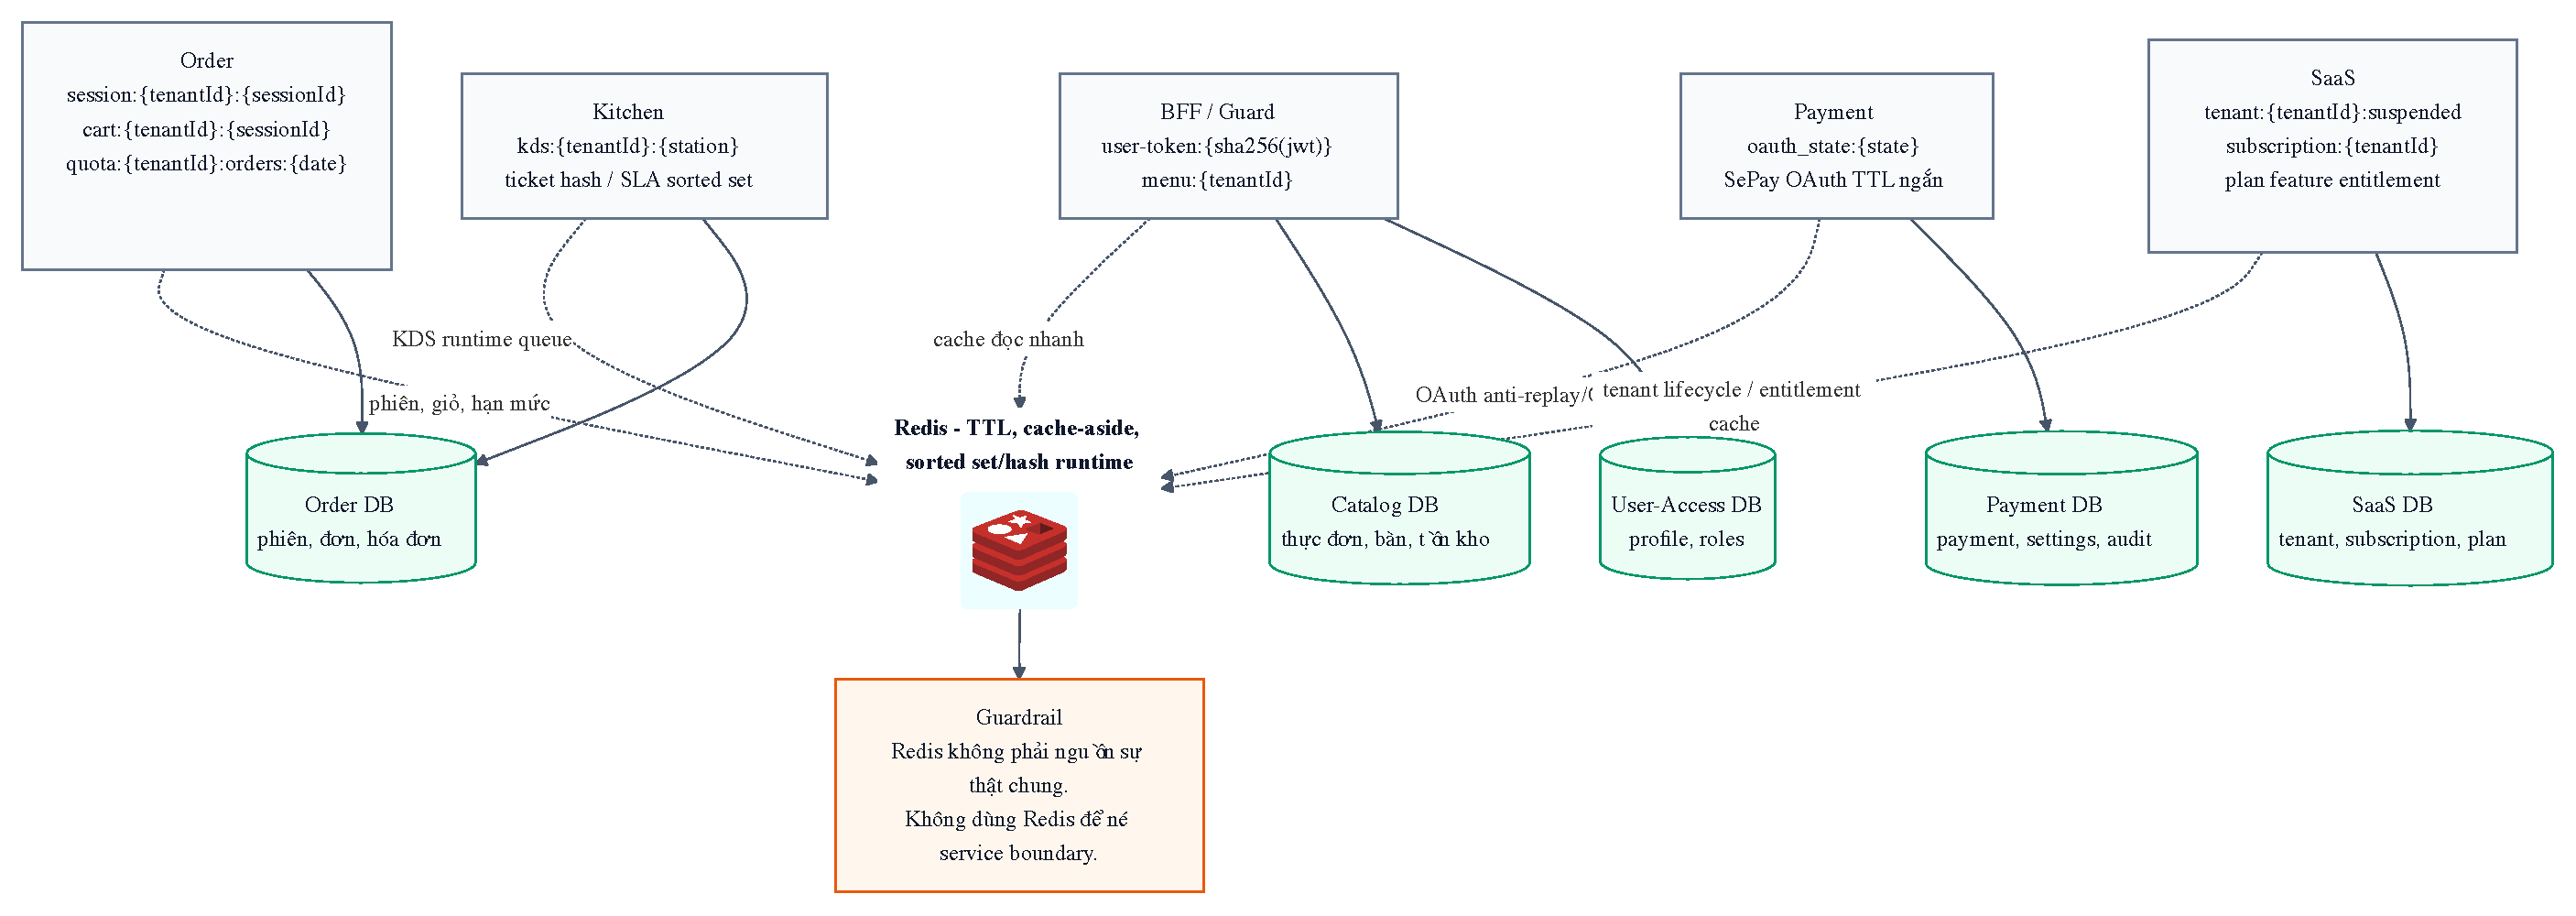
\includegraphics[width=\textwidth,height=0.82\textheight,keepaspectratio]{chapter4-redis-ownership.pdf}
  \caption{Sở hữu Redis theo nhóm khóa trong QRTable.}
  \label{fig:chapter4-redis-ownership}
\end{figure}

\subsection{Các nhóm khóa và cấu trúc dữ liệu Redis}

Bảng~\ref{tab:chapter4-redis-data-structures} tóm tắt các nhóm Redis chính theo chủ sở hữu, mẫu khóa (key pattern), kiểu dữ liệu và nguồn sự thật. Bảng này bổ sung cho Hình~\ref{fig:chapter4-redis-ownership}: hình cho thấy ranh giới sở hữu, còn bảng cho thấy cấu trúc dữ liệu cụ thể được chọn cho từng trường hợp sử dụng.

{\scriptsize
\setlength{\tabcolsep}{1pt}
\begin{longtable}{>{\raggedright\arraybackslash}p{0.12\textwidth}>{\raggedright\arraybackslash}p{0.08\textwidth}>{\raggedright\arraybackslash}p{0.16\textwidth}>{\raggedright\arraybackslash}p{0.1\textwidth}>{\raggedright\arraybackslash}p{0.13\textwidth}>{\raggedright\arraybackslash}p{0.11\textwidth}>{\raggedright\arraybackslash}p{0.16\textwidth}}
  \caption{Sở hữu Redis và cấu trúc dữ liệu theo nhóm sử dụng.}
  \label{tab:chapter4-redis-data-structures}\\
  \toprule
  Nhóm dữ liệu & Chủ sở hữu & Mẫu khóa & Kiểu Redis & Vòng đời / TTL & Nguồn sự thật & Vai trò kiến trúc \\
  \midrule
  \endfirsthead
  \toprule
  Nhóm dữ liệu & Chủ sở hữu & Mẫu khóa & Kiểu Redis & Vòng đời / TTL & Nguồn sự thật & Vai trò kiến trúc \\
  \midrule
  \endhead
  \bottomrule
  \endfoot
  Bộ nhớ đệm thực đơn công khai & Catalog / BFF & \texttt{menu:\{tenantId\}} & Chuỗi / JSON đệm & Xóa khi danh mục/món đổi. & Catalog PostgreSQL & Giảm tải đường đọc thực đơn công khai. \\
  Phiên khi vận hành & Order & \texttt{session:}\newline\texttt{\{tenantId\}:}\newline\texttt{\{sessionId\}} & Hash & TTL phiên; xóa khi đóng/giải phóng. & Order PostgreSQL & Đường xử lý tần suất cao (hot path) cho phiên QR và kiểm tra phiên đang hoạt động. \\
  Giỏ chung & Order & \texttt{cart:\{tenantId\}:}\newline\texttt{\{sessionId\}} & Hash với \texttt{items} JSON & TTL theo phiên; xóa/khóa khi gửi đơn hoặc lập hóa đơn. & Order khi vận hành; CSDL Order sau khi gửi đơn & Giỏ chung nhiều khách, có \texttt{cartVersion} để phát hiện xung đột. \\
  Hạn mức đơn theo ngày & Ranh giới Order / SaaS & \texttt{quota:}\newline\texttt{\{tenantId\}:}\newline\texttt{orders:\{date\}} & Bộ đếm / Chuỗi & Cửa sổ theo ngày, TTL khoảng 48 giờ. & Quyền lợi gói Order/SaaS & Kiểm soát hạn mức đơn theo gói thuê bao. \\
  Bộ nhớ đệm gói thuê bao & SaaS & \texttt{subscription:}\newline\texttt{\{tenantId\}} & Chuỗi / JSON & TTL 300 giây. & SaaS PostgreSQL & Đọc nhanh gói, quyền lợi gói và giới hạn gói. \\
  Cờ tạm ngưng & SaaS & \texttt{tenant:}\newline\texttt{\{tenantId\}:}\newline\texttt{suspended} & Cờ chuỗi & Bật/tắt theo vòng đời đơn vị thuê bao. & SaaS PostgreSQL & Guard ở BFF có cờ nhanh khi đơn vị thuê bao bị tạm ngưng. \\
  Trạng thái OAuth & Payment & \texttt{oauth\_state:}\newline\texttt{\{state\}} & Chuỗi / JSON & TTL 300 giây, dùng một lần. & Luồng OAuth Payment / CSDL cấu hình & Chống phát lại và gắn callback SePay với đơn vị thuê bao/chủ sở hữu. \\
  KDS khi vận hành & Kitchen & \texttt{kds:*}, \texttt{lock:kds:*}, \texttt{realtime:kds:*} & Hash, Set, Sorted Set, List, Chuỗi, Pub/Sub & Theo phiếu, SLA và dọn dẹp. & Sự kiện Order + bản chiếu Kitchen & Hàng đợi bếp/bar, SLA, khử trùng và phát tán thời gian thực. \\
\end{longtable}
}

Bộ nhớ đệm thực đơn phục vụ thực đơn công khai và giảm số lần truy vấn Catalog cho các yêu cầu đọc lặp lại từ khách. BFF có thể lưu đệm hoặc làm mất hiệu lực thực đơn sau khi sửa đổi, nhưng CSDL Catalog vẫn là nguồn sự thật. Phiên và giỏ do Order quản lý: \texttt{session:\{tenantId\}:\{sessionId\}} là hash phản chiếu thông tin phiên đang hoạt động, còn \texttt{cart:\{tenantId\}:\{sessionId\}} lưu giỏ chung, trạng thái khóa và phiên bản \texttt{cartVersion}. Khi nhiều khách cùng bàn thao tác, phiên bản giỏ giúp phát hiện xung đột thay vì ghi đè im lặng. Hết hạn Redis không tự động có nghĩa đơn/phiên nghiệp vụ đã biến mất; Order vẫn là nơi quyết định đóng phiên, giải phóng bàn và xóa giỏ khi đủ điều kiện.

SaaS dùng Redis cho cờ tạm ngưng đơn vị thuê bao và bộ nhớ đệm gói thuê bao để BFF/guard có thể đọc nhanh trạng thái vận hành. Payment dùng bộ nhớ đệm trạng thái OAuth với TTL ngắn để chống phát lại/CSRF trong SePay OAuth Connect. Các khóa này hỗ trợ đường xử lý tần suất cao, nhưng cơ sở dữ liệu của dịch vụ sở hữu vẫn là nơi lưu trạng thái bền vững.

\subsection{Ví dụ minh họa KDS: hàng đợi theo trạm bếp/bar}

KDS là trường hợp dùng Redis sâu nhất trong QRTable. Kitchen không có CSDL bền vững riêng trong phạm vi hiện tại. Thay vào đó, Kitchen tiêu thụ sự kiện xác nhận đơn, dựng bản chiếu phiếu theo trạm bếp/bar và lưu trạng thái khi vận hành trong Redis. Mô hình này phù hợp với yêu cầu hàng đợi thời gian thực: cần sắp xếp FIFO, ưu tiên, chuyển trạng thái phiếu, cảnh báo SLA, khử trùng và phát gợi ý cho client nhanh sau mỗi thay đổi trạng thái.

{\scriptsize
\setlength{\tabcolsep}{1pt}
\begin{longtable}{>{\raggedright\arraybackslash}p{0.25\textwidth}>{\raggedright\arraybackslash}p{0.11\textwidth}>{\raggedright\arraybackslash}p{0.19\textwidth}>{\raggedright\arraybackslash}p{0.18\textwidth}>{\raggedright\arraybackslash}p{0.2\textwidth}}
  \caption{Cấu trúc dữ liệu Redis trong ví dụ minh họa KDS.}
  \label{tab:chapter4-kds-redis-data-structures}\\
  \toprule
  Mẫu khóa & Kiểu & Nội dung / thành viên & Mục đích & Ghi chú consistency \\
  \midrule
  \endfirsthead
  \toprule
  Mẫu khóa & Kiểu & Nội dung / thành viên & Mục đích & Ghi chú consistency \\
  \midrule
  \endhead
  \bottomrule
  \endfoot
  \texttt{kds:\{tenantId\}:}\newline\texttt{ticket:\{ticketId\}} & Hash & Siêu dữ liệu phiếu, trạng thái, trạm, SLA, phiên bản. & Bản ghi chạy chính của phiếu KDS. & Sinh từ \texttt{order.confirmed}; không thay thế lịch sử Order. \\
  \texttt{kds:\{tenantId\}:}\newline\texttt{ticket-item:\{ticketItemId\}} & Hash & Món trong phiếu, số lượng, trạng thái món. & Theo dõi từng món trong bếp/bar. & Món đi theo phiếu và dòng đơn gốc. \\
  \texttt{kds:\{tenantId\}:}\newline\texttt{ticket:\{ticketId\}:items} & Set & Danh sách \texttt{ticketItemId}. & Chỉ mục từ phiếu sang món. & Giúp lấy snapshot phiếu mà không quét toàn Redis. \\
  \texttt{kds:\{tenantId\}:}\newline\texttt{order:\{orderId\}:tickets} & Set & Danh sách phiếu thuộc đơn. & Tìm phiếu khi hủy đơn hoặc tái dựng. & Giữ liên hệ khi vận hành với aggregate Order. \\
  \texttt{kds:\{tenantId\}:}\newline\texttt{session:}\newline\texttt{\{sessionId\}:tickets} & Set & Danh sách phiếu thuộc phiên. & Cập nhật bổ sung snapshot bàn/phiên. & Tối ưu tra cứu theo phiên, không là dữ liệu nghiệp vụ bền vững. \\
  \texttt{kds:\{tenantId\}:}\newline\texttt{\{station\}} & Sorted Set & Phiếu đang hoạt động, điểm theo FIFO/ưu tiên. & Hàng đợi đang chờ/đang xử lý theo trạm. & Điểm tính từ thời điểm xác nhận và ưu tiên. \\
  \texttt{kds:\{tenantId\}:}\newline\texttt{station:\{station\}:READY} & Sorted Set & Phiếu đã sẵn sàng, điểm là thời điểm sẵn sàng. & Giữ nhóm món đã sẵn sàng cho gọi lại/hiển thị. & Không làm thay đổi nguồn sự thật của đơn. \\
  \texttt{kds:sla:due} & Sorted Set & \texttt{tenantId|station|}\newline\texttt{ticketId|level}. & Lịch cảnh báo/vượt ngưỡng SLA. & Tiến trình chiếm quyền xử lý/khử trùng trước khi phát cảnh báo. \\
  \texttt{kds:\{tenantId\}:}\newline\texttt{ticket:\{ticketId\}:sla} & Hash & Mốc cảnh báo/vượt ngưỡng và mức gần nhất. & Tra cứu SLA của phiếu. & Cập nhật cùng trạng thái phiếu khi tiến trình xử lý. \\
  \texttt{kds:\{tenantId\}:}\newline\texttt{dedupe:event:\{eventId\}} & Khóa chuỗi & Dấu đã xử lý sự kiện. & Chống xử lý lại \texttt{order.confirmed}. & TTL dài hơn vòng đời phiếu thông thường. \\
  \texttt{kds:\{tenantId\}:}\newline\texttt{dedupe:order:\{orderId\}:}\newline\texttt{\{station\}} & Khóa chuỗi & Dấu phiếu theo đơn/trạm đã tạo. & Chống tạo hai phiếu cùng trạm khi phát lại. & Khử trùng theo sự kiện và theo đơn/trạm. \\
  \texttt{kds:\{tenantId\}:}\newline\texttt{cmd:\{requestId\}} & Khóa chuỗi & Dấu lệnh đã nhận. & Idempotency cho thao tác phiếu. & Tránh nhấn đôi hoặc retry từ client. \\
  \texttt{kds:\{tenantId\}:}\newline\texttt{dead-letter:}\newline\texttt{order-confirmed} & List & Payload lỗi/sai định dạng hoặc thiếu trạm. & Lưu mẫu lỗi để điều tra. & Không dùng làm luồng xử lý chính. \\
  \texttt{lock:kds:rebuild:}\newline\texttt{\{tenantId\}} & Khóa chuỗi & Mã tái dựng snapshot. & Chống nhiều tiến trình tái dựng cùng đơn vị thuê bao. & TTL ngắn, giải phóng khi hoàn tất. \\
  \texttt{realtime:kds:}\newline\texttt{\{tenantId\}} & Pub/Sub & \texttt{kds.queue\_changed}. & Gợi ý nội bộ cho BFF phát WebSocket. & Không bền vững, không là nguồn trạng thái. \\
\end{longtable}
}

Hình~\ref{fig:chapter4-kds-redis-data-structures} trực quan hóa bảng trên. Luồng bắt đầu khi Order ghi sự kiện xác nhận đơn qua outbox giao dịch/Kafka. Kitchen tiêu thụ sự kiện, ghi các cấu trúc Redis và phát gợi ý nội bộ sau khi thay đổi trạng thái thành công. BFF chỉ nhận gợi ý này để phát WebSocket vào phòng KDS/quản trị; BFF không tự tạo phiếu và không suy luận trạng thái bếp.

\begin{figure}[H]
  \centering
  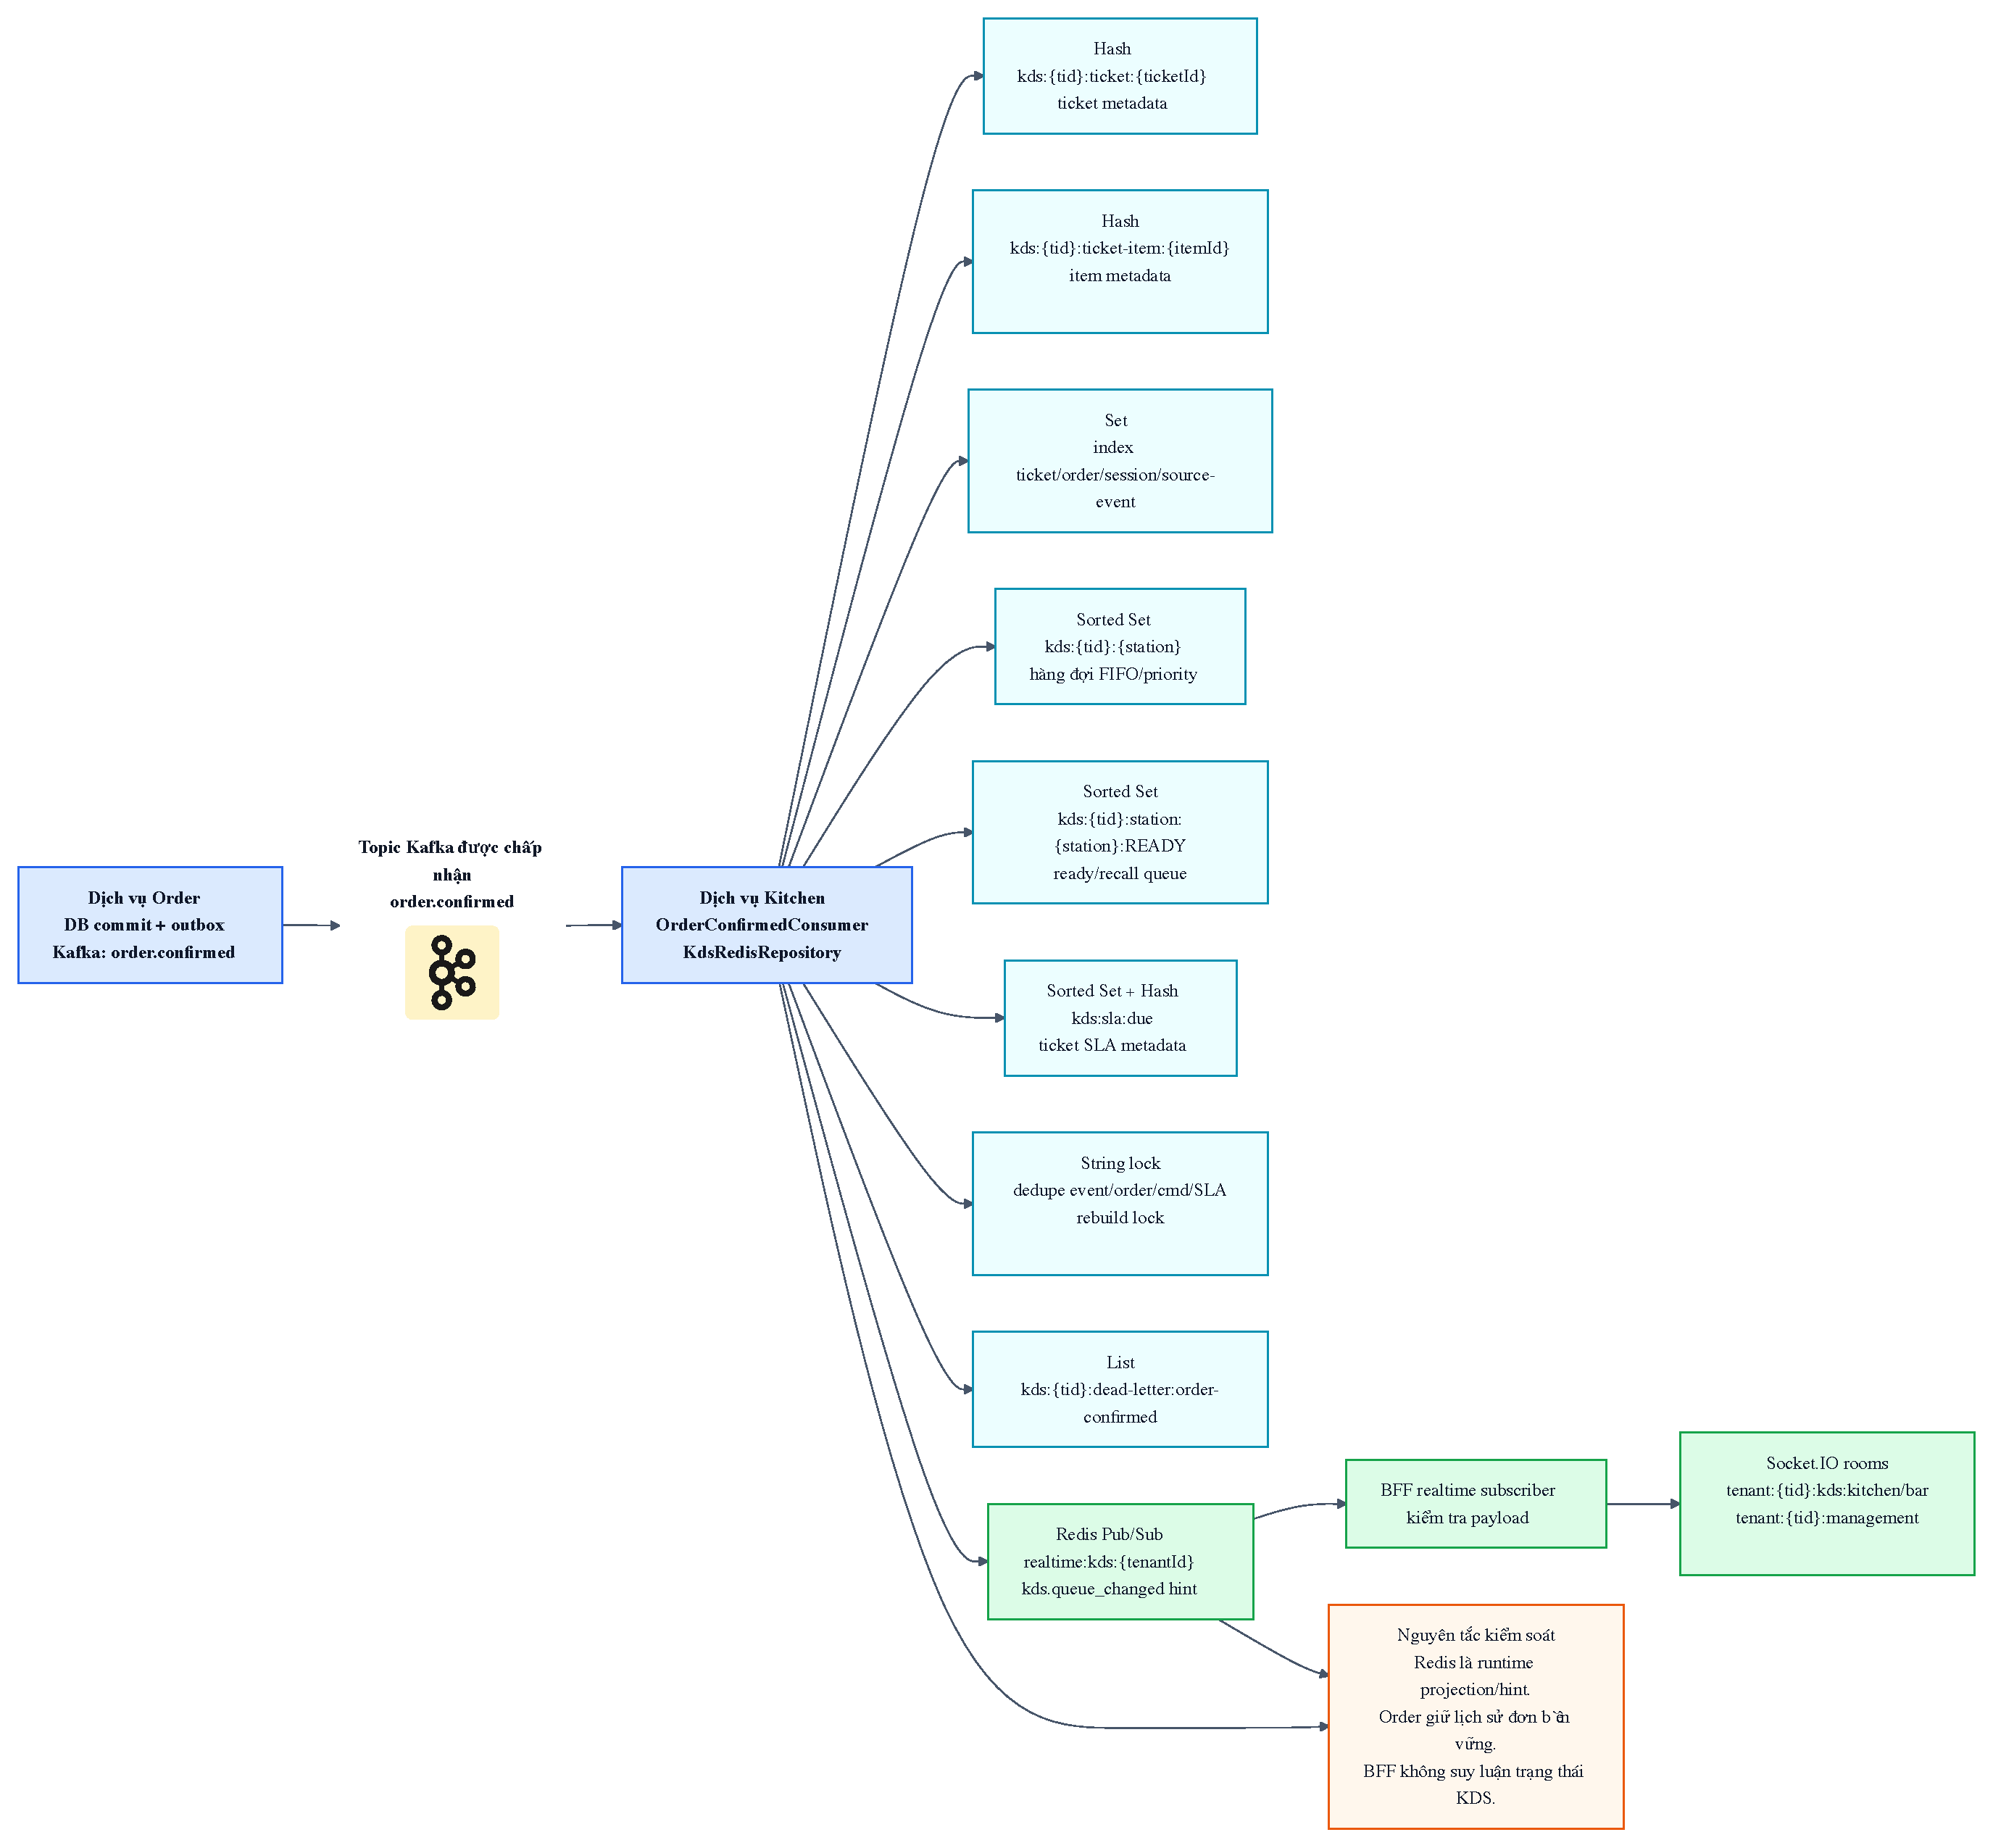
\includegraphics[width=\textwidth,height=0.82\textheight,keepaspectratio]{chapter4-kds-redis-data-structures.pdf}
  \caption{Cấu trúc dữ liệu Redis cho hàng đợi KDS và cầu nối thời gian thực.}
  \label{fig:chapter4-kds-redis-data-structures}
\end{figure}

\subsection{Redis Pub/Sub cho gợi ý thời gian thực}

Redis Pub/Sub trong KDS chỉ là kênh phát gợi ý sau khi Kitchen đã ghi xong trạng thái khi vận hành. Kitchen xuất bản vào kênh \texttt{realtime:kds:*} với loại sự kiện hàng đợi KDS thay đổi; BFF kiểm tra payload và phát Socket.IO tới phòng KDS bếp/bar hoặc phòng quản trị của đơn vị thuê bao. Vì Pub/Sub không lưu bền vững, client phải có khả năng tải lại snapshot khi mất kết nối hoặc nhận sự kiện trễ.

\subsection{Giới hạn và nguồn sự thật của dữ liệu}

Giới hạn quan trọng của thiết kế Redis là Redis không quyết định nghiệp vụ cuối cùng. Catalog PostgreSQL vẫn là nguồn sự thật của thực đơn, bàn và tồn kho; Order PostgreSQL vẫn là nguồn sự thật của phiên, đơn và hóa đơn; Payment PostgreSQL vẫn là nguồn sự thật của giao dịch và cấu hình thanh toán; SaaS PostgreSQL vẫn là nguồn sự thật của đơn vị thuê bao, gói và subscription. Riêng KDS, Redis là bản chiếu khi vận hành do Kitchen sở hữu, được dựng từ sự kiện đã commit ở Order. Nếu sau này cần kiểm toán lịch sử bếp hoặc phân tích hiệu suất chế biến lâu dài, hệ thống có thể bổ sung kho lưu trữ bền vững hoặc bản chiếu riêng cho Kitchen mà không phá vỡ ranh giới hiện tại.

\section{Kiến trúc bảo mật, xác thực và phân quyền}

Thiết kế bảo mật của QRTable xuất phát từ ranh giới tin cậy: client không được xem là nguồn đáng tin tuyệt đối; BFF là điểm vào cho HTTP/WebSocket; các dịch vụ miền chỉ nhận yêu cầu đã có ngữ cảnh hợp lệ thông qua BFF hoặc qua contract nội bộ. Nhóm nhân viên, chủ quán, quản lý và quản trị nền tảng dùng Keycloak, JWT/OIDC và RBAC. JWT là chuẩn phổ biến để truyền khẳng định danh tính và xác thực dựa trên token \cite{jones-jwt-rfc7519-2015}. Trong QRTable, Keycloak là nguồn định danh, Authorizer xác minh token, còn User-Access lưu hồ sơ ứng dụng, vai trò và ánh xạ quyền theo đơn vị thuê bao.

\subsection{Ranh giới tin cậy và mô hình tác nhân}

QRTable không dùng một mô hình xác thực duy nhất cho mọi tác nhân. Khách tại bàn cần truy cập nhanh qua QR và phiên; nhân viên vận hành cần quyền theo vai trò trong một đơn vị thuê bao; chủ quán và quản lý cần thêm quyền quản trị nội bộ; Super Admin cần quyền nền tảng có kiểm soát; SePay là nhà cung cấp ngoài gửi callback chứ không phải người dùng hệ thống. Bảng~\ref{tab:chapter4-auth-actor-model} tóm tắt mô hình này.

{\scriptsize
\setlength{\tabcolsep}{3pt}
\begin{longtable}{>{\raggedright\arraybackslash}p{0.13\textwidth}>{\raggedright\arraybackslash}p{0.16\textwidth}>{\raggedright\arraybackslash}p{0.17\textwidth}>{\raggedright\arraybackslash}p{0.19\textwidth}>{\raggedright\arraybackslash}p{0.2\textwidth}}
  \caption{Mô hình tác nhân và cơ chế xác thực trong QRTable.}
  \label{tab:chapter4-auth-actor-model}\\
  \toprule
  Tác nhân & Điểm vào & Cơ chế xác thực & Phạm vi truy cập & Ghi chú kiến trúc \\
  \midrule
  \endfirsthead
  \toprule
  Tác nhân & Điểm vào & Cơ chế xác thực & Phạm vi truy cập & Ghi chú kiến trúc \\
  \midrule
  \endhead
  Customer & Customer PWA qua BFF & QR/table token và phiên & Bàn, phiên và đơn vị thuê bao hiện tại & Không có role RBAC trong \texttt{role.json}; hành vi bị giới hạn bởi session/ownership. \\
  Waiter/\newline Chef/\newline Barista & Management App qua BFF & Keycloak, JWT/OIDC & Một đơn vị thuê bao & Quyền thao tác đến từ permission set, ví dụ xác nhận đơn hoặc cập nhật KDS. \\
  Owner/\newline Manager & Management App qua BFF & Keycloak, JWT/OIDC & Một đơn vị thuê bao, kèm quyền quản trị theo role & Một số chức năng quản trị/báo cáo còn phụ thuộc entitlement của gói dịch vụ. \\
  Super Admin & Management App admin qua BFF & Keycloak, JWT/OIDC & Nền tảng và thao tác nhiều đơn vị thuê bao có kiểm soát & Quyền nền tảng không đồng nghĩa bỏ toàn bộ kiểm soát hoặc kiểm toán. \\
  SePay webhook/\newline OAuth callback & HTTP callback vào BFF & Secret/header,\newline reference hoặc OAuth state & Payment hoặc SaaS tùy tuyến và tiền tố tham chiếu & Là external integration boundary, không phải user flow. \\
  \bottomrule
\end{longtable}
}

\subsection{Hai luồng xác thực: nhân viên/quản trị và khách tại bàn}

Hình~\ref{fig:chapter4-security-auth-flow} đặt hai luồng này cạnh nhau. Luồng nhân viên/chủ quán/quản trị đi qua Keycloak, Authorizer, User-Access và chuỗi guard của BFF. Luồng khách bắt đầu từ QR/phiên, đi qua SessionGuard và TenantGuard, sau đó chỉ được truy cập các thao tác phù hợp với phiên/bàn hiện tại. Sự tách biệt này là lý do chương không mô tả khách như một người dùng Keycloak.

\begin{figure}[H]
  \centering
  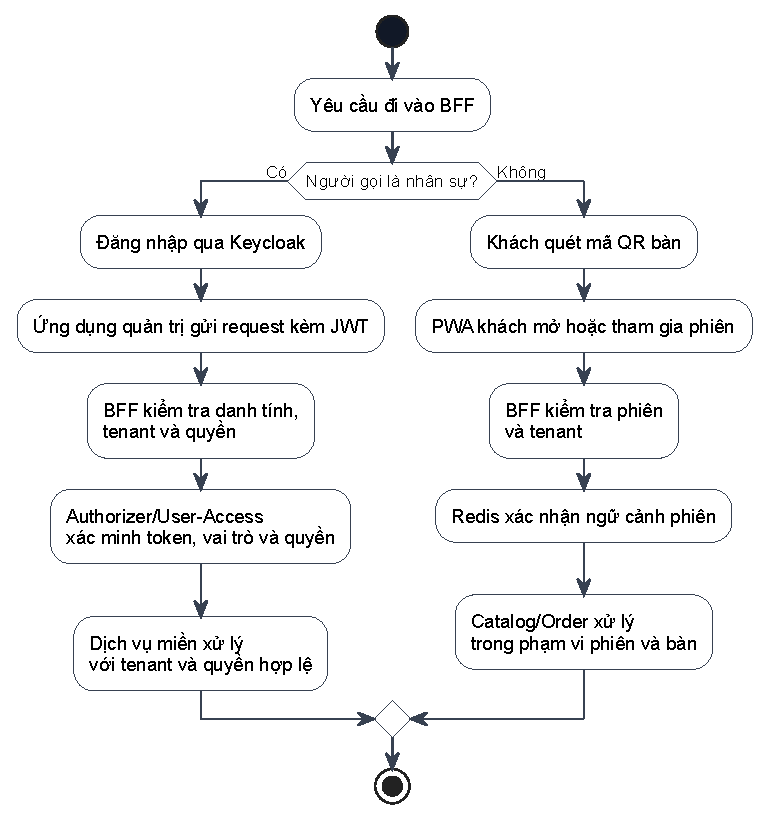
\includegraphics[width=\textwidth,height=0.82\textheight,keepaspectratio]{chapter4-security-auth-flow.pdf}
  \caption{Kiến trúc xác thực và phân quyền cho nhân viên/quản trị và khách tại bàn.}
  \label{fig:chapter4-security-auth-flow}
\end{figure}

Khách không dùng Keycloak. Khách là tác nhân ẩn danh theo phiên, bắt đầu từ URL QR có token bàn và sau đó đi qua guard phiên. Quyết định này phù hợp với bối cảnh F\&B: khách tại bàn cần truy cập nhanh, không nên bị buộc đăng nhập tài khoản chỉ để xem thực đơn hoặc đặt món. Bảo mật của luồng khách dựa trên token QR, HMAC, quyền sở hữu phiên, ngữ cảnh đơn vị thuê bao và giới hạn hành vi theo phiên tại bàn. Session trong ngữ cảnh này không đồng nghĩa tài khoản người dùng; nó là ràng buộc ngắn hạn giữa đơn vị thuê bao, bàn, phiên và các thao tác được phép.

\subsection{Request context và chuỗi kiểm soát tại BFF}

Chuỗi guard ở BFF giúp tách các câu hỏi bảo mật thành nhiều lớp. UserGuard hoặc SessionGuard trả lời ``người gọi là ai'', TenantGuard trả lời ``yêu cầu thuộc đơn vị thuê bao nào'', PermissionGuard trả lời ``tác nhân có quyền thực hiện hành động này không'', còn PlanFeatureGuard trả lời ``đơn vị thuê bao có được dùng tính năng này theo gói không''. Bảng~\ref{tab:chapter4-security-control-layers} diễn đạt các lớp này như request context và câu hỏi kiến trúc, thay vì phân tích từng method của framework.

{\scriptsize
\setlength{\tabcolsep}{3pt}
\begin{longtable}{>{\raggedright\arraybackslash}p{0.17\textwidth}>{\raggedright\arraybackslash}p{0.25\textwidth}>{\raggedright\arraybackslash}p{0.2\textwidth}>{\raggedright\arraybackslash}p{0.24\textwidth}}
  \caption{Các lớp kiểm soát bảo mật tại BFF và ngữ cảnh yêu cầu.}
  \label{tab:chapter4-security-control-layers}\\
  \toprule
  Lớp kiểm soát & Câu hỏi kiến trúc & Áp dụng cho & Kết quả mong muốn \\
  \midrule
  \endfirsthead
  \toprule
  Lớp kiểm soát & Câu hỏi kiến trúc & Áp dụng cho & Kết quả mong muốn \\
  \midrule
  \endhead
  Xác định actor & Người gọi là staff/admin hay customer session? & HTTP/WebSocket từ client & Có identity hoặc session context trước khi xử lý. \\
  Khóa đơn vị thuê bao & Request đang thuộc \texttt{tenantId} nào? & Hầu hết API tenant-scoped & Không để tác nhân của đơn vị thuê bao A truy cập dữ liệu của đơn vị thuê bao B. \\
  Kiểm tra quyền thao tác & Tác nhân có permission cho hành động không? & API staff/owner/admin & Ngăn role không phù hợp thao tác menu, order, payment hoặc report. \\
  Kiểm tra quyền theo gói & Đơn vị thuê bao có tính năng trong subscription không? & Dashboard/reporting và feature-gated routes & Phân biệt entitlement thương mại với RBAC của người dùng. \\
  Kiểm tra phiên/bàn & Session có khớp bàn, đơn vị thuê bao và trạng thái hợp lệ không? & Customer PWA & Giữ khách trong phạm vi phiên hiện tại. \\
  Định tuyến external callback & Webhook/OAuth callback có đúng tuyến, secret/header, reference hoặc state không? & SePay webhook/OAuth callback & Chuyển đúng Payment hoặc SaaS, hỗ trợ xử lý idempotency và audit. \\
  \bottomrule
\end{longtable}
}

BFF gom các cross-cutting security concern như xác thực, ngữ cảnh đơn vị thuê bao, permission, entitlement, định tuyến webhook và cầu nối thời gian thực. Tuy nhiên, BFF không trở thành nơi quyết định bất biến nghiệp vụ cốt lõi. Trạng thái đơn, tồn kho, thanh toán, gói thuê bao và dữ liệu báo cáo vẫn thuộc về dịch vụ sở hữu tương ứng.

\subsection{RBAC, tenant isolation và quyền theo gói}

Ba khái niệm trong mục này dễ bị trộn lẫn nếu chỉ nhìn qua tên guard. RBAC kiểm tra người dùng có quyền thực hiện hành động hay không; tenant isolation khóa dữ liệu và hành động vào một đơn vị thuê bao hợp lệ; quyền theo gói dịch vụ kiểm tra đơn vị thuê bao có được dùng tính năng hay không. Bảng~\ref{tab:chapter4-rbac-tenant-entitlement} tách ba lớp này và bổ sung quyền nền tảng của Super Admin.

{\scriptsize
\setlength{\tabcolsep}{3pt}
\begin{longtable}{>{\raggedright\arraybackslash}p{0.17\textwidth}>{\raggedright\arraybackslash}p{0.25\textwidth}>{\raggedright\arraybackslash}p{0.24\textwidth}>{\raggedright\arraybackslash}p{0.2\textwidth}}
  \caption{Phân biệt RBAC, cô lập đơn vị thuê bao và quyền theo gói dịch vụ.}
  \label{tab:chapter4-rbac-tenant-entitlement}\\
  \toprule
  Cơ chế & Trả lời câu hỏi & Ví dụ trong QRTable & Giới hạn diễn giải \\
  \midrule
  \endfirsthead
  \toprule
  Cơ chế & Trả lời câu hỏi & Ví dụ trong QRTable & Giới hạn diễn giải \\
  \midrule
  \endhead
  RBAC & Người dùng có quyền làm hành động này không? & Waiter được xác nhận đơn; Chef/Barista xem và cập nhật KDS; Owner quản lý menu/staff. & Không tự quyết định đơn vị thuê bao hoặc gói dịch vụ. \\
  Tenant isolation & Dữ liệu/hành động thuộc đơn vị thuê bao nào? & API, DB query, Redis key, Kafka payload và WebSocket room đều mang ngữ cảnh \texttt{tenantId}. & Không phải cơ sở dữ liệu riêng cho từng đơn vị thuê bao trong thiết kế hiện tại. \\
  Plan entitlement & Đơn vị thuê bao có được dùng tính năng này theo gói không? & Owner/Manager có \texttt{report.read\_own}, nhưng báo cáo nâng cao còn phụ thuộc \texttt{analytics\_basic}. & Không phải role người dùng. \\
  Platform permission & Super Admin có quyền nền tảng nào? & Onboard tenant, quản lý plan, xem platform analytics và tenant drilldown có kiểm soát. & Không phải quyền tự do bỏ qua mọi kiểm soát hoặc audit. \\
  \bottomrule
\end{longtable}
}

Ma trận permission đầy đủ của QRTable nằm ở tài liệu kiến trúc RBAC, không được lặp toàn bộ trong chương chính. Về thiết kế, điểm cần nhấn mạnh là Customer không nằm trong \texttt{role.json}; khách được bảo vệ bằng session/ownership. Ngược lại, staff/owner/manager/super admin dùng role/permission do Keycloak và User-Access phối hợp cung cấp cho BFF.

\subsection{WebSocket và webhook trong mô hình bảo mật}

WebSocket trong QRTable không phải nguồn quyền và cũng không phải nguồn trạng thái có thẩm quyền. Socket chỉ được join room sau khi có auth/session context phù hợp: staff đi theo token và \texttt{tenantId}; khách đi theo session và \texttt{tenantId}; KDS đi theo room của đơn vị thuê bao và trạm bếp/bar. Khi nhận gợi ý thời gian thực, client vẫn phải có khả năng tải lại snapshot qua API nếu cần trạng thái chính xác.

Bảo mật cũng xuất hiện ở webhook thanh toán. QRTable phân biệt các tuyến webhook của SePay theo tầng: tuyến HMAC tương thích, tuyến hóa đơn nhà hàng và tuyến hóa đơn gói nền tảng. Hóa đơn nhà hàng dùng tiền tố \texttt{QRTBL}, hóa đơn gói dùng tiền tố \texttt{QRSUB}. BFF xác thực tuyến và header phù hợp trước khi chuyển payload đến Payment hoặc SaaS. OAuth callback được ràng buộc bằng state ngắn hạn để gắn quá trình kết nối SePay với đúng đơn vị thuê bao/chủ sở hữu.

\subsection{Giới hạn thiết kế và phạm vi khẳng định}

Phần bảo mật của Chương 4 trình bày thiết kế và ranh giới kiểm soát, không thay thế đánh giá kiểm thử ở Chương 6. QRTable có cơ sở để nói rằng kiến trúc đã tách hai luồng xác thực, có guard chain cho nhân viên/khách, có permission matrix cho sáu role staff/admin, có session-scoped customer actor, có entitlement cho dashboard/reporting và có contract webhook theo tuyến. Tuy nhiên, chương này không khẳng định đã có kiểm thử xâm nhập chính thức, tự động xoay vòng bí mật, mTLS nội bộ, service mesh, WAF hoặc bằng chứng phủ toàn bộ bề mặt API liên đơn vị thuê bao. Kết quả kiểm chứng các điểm này được trình bày thận trọng trong Chương~\ref{chap:danh-gia}.

\section{Thiết kế tích hợp thanh toán SePay/VietQR}

Mô hình thanh toán của QRTable phản ánh hai dòng tiền khác nhau. Dòng tiền thứ nhất là khách trả tiền hóa đơn cho nhà hàng. Dòng này dùng tiền tố tham chiếu \texttt{QRTBL}; Payment sở hữu bản ghi thanh toán, cấu hình thanh toán của đơn vị thuê bao, trạng thái kết nối SePay và quyết toán webhook. Dòng tiền thứ hai là đơn vị thuê bao trả phí gói thuê bao cho nền tảng. Dòng này dùng tiền tố \texttt{QRSUB}; SaaS sở hữu hóa đơn gói và xử lý trạng thái gói thuê bao.

Hình~\ref{fig:chapter4-sepay-payment-architecture} minh họa hai dòng tiền trên cùng một nhà cung cấp thanh toán nhưng khác chủ sở hữu nghiệp vụ. Dòng \texttt{QRTBL} đi qua Payment để quyết toán hóa đơn nhà hàng rồi phối hợp với Order; dòng \texttt{QRSUB} đi qua SaaS để kích hoạt hoặc cập nhật gói thuê bao. BFF giữ vai trò xác thực và định tuyến webhook theo tầng, không làm chủ sở hữu trạng thái thanh toán.

\begin{figure}[H]
  \centering
  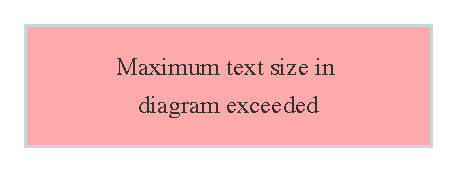
\includegraphics[width=\textwidth,height=0.82\textheight,keepaspectratio]{chapter4-sepay-payment-architecture.pdf}
  \caption{Luồng thanh toán SePay/VietQR cho hóa đơn nhà hàng và gói thuê bao.}
  \label{fig:chapter4-sepay-payment-architecture}
\end{figure}

Việc tách hai tầng giúp tránh nhầm lẫn trách nhiệm. Payment không sở hữu vòng đời gói thuê bao của đơn vị thuê bao, còn SaaS không sở hữu từng bản ghi thanh toán của hóa đơn nhà hàng. BFF định tuyến webhook dựa trên tuyến và mã thanh toán để chuyển đúng bộ xử lý. Với hóa đơn của khách, Payment xử lý quyết toán và sau đó phối hợp với Order để đánh dấu hóa đơn đã thanh toán. Với hóa đơn gói, SaaS xử lý việc kích hoạt/cập nhật gói sau khi xác nhận thanh toán.

Luồng VietQR cũng phải giữ nguyên tắc idempotency. Một webhook từ nhà cung cấp có thể đến trễ, đến nhiều lần hoặc thiếu trường nhận dạng trong một số tình huống. Payment/SaaS cần khớp tham chiếu trong \texttt{code}, \texttt{content} hoặc dữ liệu liên quan, kiểm tra số tiền, ghi kiểm toán và chỉ chuyển trạng thái khi đủ điều kiện. Phần này mô tả thiết kế tích hợp và ranh giới kiểm soát; kết quả kiểm chứng nhà cung cấp thật, webhook giả lập hoặc kiểm thử thủ công sẽ thuộc Chương 6.

\section{Thiết kế triển khai và giới hạn khẳng định}

QRTable có thiết kế chạy bằng Docker/Docker Compose cùng các thành phần phụ thuộc như PostgreSQL, MongoDB, Redis, Kafka và Keycloak. Thiết kế này giúp gom môi trường phát triển/trình diễn vào một bộ môi trường có thể tái lập, giảm chênh lệch giữa máy phát triển và môi trường trình diễn.

Tuy nhiên, thiết kế triển khai không đồng nghĩa hệ thống đã đạt sẵn sàng cao, kiểm thử áp lực dưới tải lớn hoặc kiểm thử gây lỗi có chủ đích. Trong phạm vi Chương 4, triển khai được trình bày như nền tảng cho trình diễn và thu thập hiện vật production. Các khẳng định về thời gian hoạt động, thông lượng, khả năng phục hồi hoặc vận hành cấp doanh nghiệp chỉ phù hợp khi có minh chứng kiểm chứng riêng.

\section{Tổng hợp đánh đổi kiến trúc}

Quyết định dùng vi dịch vụ thay vì một khối ứng dụng duy nhất giúp QRTable tách rõ các ngữ cảnh giới hạn có nhịp thay đổi khác nhau: Catalog/tồn kho, Order/phiên/hóa đơn, Kitchen/KDS, Payment/quyết toán, SaaS/gói thuê bao và User-Access/RBAC. Lợi ích chính là trách nhiệm dữ liệu rõ hơn, giảm phụ thuộc chéo miền nghiệp vụ và dễ trình bày/đánh giá từng luồng theo ranh giới dịch vụ. Đổi lại, hệ thống phải xử lý độ phức tạp phân tán: lỗi mạng, nhất quán cuối cùng (eventual consistency), idempotency, truy vết và lệch contract. Vì vậy, vi dịch vụ trong QRTable được dùng như một lựa chọn thiết kế có đánh đổi, không phải khẳng định luôn tốt hơn kiến trúc nguyên khối.

Quyết định kết hợp RPC đồng bộ và Kafka cũng là một đánh đổi. TCP/gRPC đơn giản hơn cho lệnh/truy vấn cần phản hồi tức thời và lỗi rõ ràng với người dùng. Kafka phù hợp hơn cho sự kiện miền bất đồng bộ, tách thời gian và phân phối. Nếu dùng Kafka cho mọi yêu cầu, hệ thống sẽ khó gỡ lỗi hơn và tăng độ trễ cho luồng khách/nhân viên. Nếu chỉ dùng RPC, các tác dụng phụ như phiếu KDS, hoàn tất thanh toán hoặc cảnh báo SLA sẽ dễ bị siết chặt với dịch vụ phát sự kiện. Khung quyết định ở Hình~\ref{fig:chapter4-kafka-decision-flow} là cách QRTable giữ cân bằng giữa hai hướng này.

Quyết định dùng Redis cho bộ nhớ đệm/phiên/KDS giúp tăng tốc các luồng tần suất cao và hỗ trợ cấu trúc hàng đợi thời gian thực. Nhưng Redis không được dùng như lối tắt để bỏ qua trách nhiệm dịch vụ. Với thực đơn, CSDL Catalog vẫn là nguồn sự thật; với phiên/giỏ, Order vẫn quyết định vòng đời; với KDS, Kitchen sở hữu bản chiếu khi vận hành; với tạm ngưng đơn vị thuê bao, SaaS sở hữu trạng thái bền vững.

Quyết định dùng cơ sở dữ liệu riêng theo dịch vụ kết hợp \texttt{tenant\_id} phù hợp với mục tiêu SaaS và phiên bản khả dụng tối thiểu của khóa luận vì giảm chi phí vận hành và vẫn giữ được truy cập dữ liệu theo đơn vị thuê bao. Hạn chế là mức cô lập vật lý giữa các đơn vị thuê bao chưa bằng cơ sở dữ liệu riêng cho từng đơn vị thuê bao. Đây là đánh đổi có thể chấp nhận trong phạm vi hiện tại, đồng thời mở đường cho mô hình cô lập lai nếu hệ thống cần phục vụ đơn vị thuê bao lớn hơn hoặc yêu cầu tuân thủ nghiêm ngặt hơn.

Cuối cùng, WebSocket được chọn để cải thiện trải nghiệm thời gian thực nhưng không được dùng làm nguồn trạng thái đáng tin. Thiết kế gợi ý/làm mới cho phép client phản hồi nhanh khi có sự kiện đơn, KDS, thanh toán hoặc vòng đời đơn vị thuê bao, đồng thời vẫn cho phép phía người dùng tái đồng bộ bằng REST/truy vấn khi mất kết nối. Tóm lại, kiến trúc QRTable hướng tới sự cân bằng giữa tách biệt theo miền nghiệp vụ và khả năng triển khai/đánh giá trong phạm vi khóa luận.

\chapter{Hiện thực các luồng vận hành cốt lõi của QRTable}

Chương này trình bày cách QRTable được hiện thực từ thiết kế ở Chương 4 thành các luồng vận hành có thể kiểm chứng. Thay vì đi theo hướng hướng dẫn sử dụng hoặc liệt kê lớp, hàm và cây thư mục mã nguồn, chương chọn các luồng đại diện để chứng minh rằng các quyết định về ranh giới dịch vụ, quyền sở hữu dữ liệu, cô lập đơn vị thuê bao (tenant isolation), tính lũy đẳng (idempotency), Saga, Redis, Kafka và WebSocket đã có dấu vết triển khai trong hệ thống.

Các luồng được chọn gồm: khách quét QR và dùng giỏ món chung; nhân viên xác nhận đơn và bảo toàn tồn kho; màn hình bếp Kitchen Display System (KDS) nhận phiếu bếp từ sự kiện; ghi nhận thanh toán tiền mặt/VietQR/SePay; khởi tạo đơn vị thuê bao theo mô hình SaaS; bảng điều khiển và báo cáo theo gói dịch vụ. Mỗi luồng được trình bày theo cùng một mạch: mục tiêu nghiệp vụ, bất biến cần giữ, dịch vụ sở hữu dữ liệu, bằng chứng triển khai và ranh giới kỹ thuật cần dùng khi đánh giá kết quả.

\section{Mục tiêu triển khai và phạm vi minh chứng}

Vai trò của Chương 5 là nối Chương 4 với hệ thống đã được xây dựng. Chương 4 đã xác định rằng QRTable tách cơ sở dữ liệu theo ranh giới dịch vụ, giữ BFF ở vai trò điểm vào và dùng WebSocket như tín hiệu gợi ý/tải lại thay cho nguồn trạng thái có thẩm quyền. Vì vậy, khi đi vào triển khai, câu hỏi chính là từng luồng giữ ranh giới sở hữu dữ liệu và bất biến nghiệp vụ như thế nào.

Phạm vi minh chứng trong chương này tập trung vào các bằng chứng nội bộ: cấu trúc dịch vụ, đăng ký mô-đun, thực thể/lược đồ dữ liệu đang được dùng, hợp đồng TCP/Kafka, kiểm thử đơn vị, kiểm thử hợp đồng, kiểm thử tích hợp có điều kiện, sơ đồ luồng vận hành và các tài liệu kỹ thuật đã được đồng bộ. Các ảnh chụp client minh họa bề mặt vận hành, còn bằng chứng về ranh giới giao dịch, tính lũy đẳng, lọc theo đơn vị thuê bao và bù trừ (compensation) đến từ mã nguồn, kiểm thử và sơ đồ.

Chương này cũng giữ ranh giới với Chương 6. Chương 5 mô tả cách hệ thống được hiện thực, đóng gói và chuẩn bị bằng chứng triển khai; Chương 6 sử dụng các bằng chứng đó để phân loại kết quả kiểm chứng của kiểm thử tự động, provider SePay thật và lớp triển khai production.

\section{Nền tảng triển khai và ranh giới trách nhiệm}

QRTable được triển khai trong một Nx monorepo gồm các ứng dụng phía người dùng, BFF và các dịch vụ nghiệp vụ. Customer PWA phục vụ khách tại bàn qua mã QR/phiên gọi món; Management App phục vụ nhân viên, bếp/bar, chủ quán, quản lý và quản trị nền tảng. Hai ứng dụng này không gọi trực tiếp các dịch vụ nghiệp vụ, mà đi qua BFF để giữ chuỗi guard, ngữ cảnh đơn vị thuê bao, phân quyền và cổng WebSocket thống nhất.

Ở lớp dịch vụ, Authorizer xác minh JWT/OIDC và tích hợp Keycloak; User-Access lưu hồ sơ ứng dụng và vai trò nghiệp vụ; Catalog sở hữu thực đơn, bàn, token QR và tồn kho; Order sở hữu phiên, giỏ, đơn, dòng đơn, hóa đơn và yêu cầu phục vụ; Kitchen sở hữu bản chiếu KDS khi vận hành; Payment sở hữu giao dịch, nhật ký kiểm toán và cấu hình thanh toán; SaaS sở hữu đơn vị thuê bao, gói giá, thuê bao, hóa đơn thuê bao và quyền theo gói. Các bảng/bộ sưu tập tương ứng đã được trình bày ở Bảng~\ref{tab:chapter4-data-ownership-schema}; Chương 5 chỉ nhắc lại dữ liệu khi nó giúp giải thích một luồng cụ thể.

Các thư viện dùng chung trong monorepo được dùng như lớp hợp đồng giữa các phần của hệ thống. Dịch vụ có thể dùng chung DTO, enum, provider token, bộ dựng khóa Redis, bộ dựng phòng WebSocket, guard hoặc kiểu phía client. Khi cần dữ liệu thuộc ngữ cảnh nghiệp vụ có ranh giới khác, dịch vụ đi qua TCP/gRPC hoặc Kafka. Chính cách dùng này giúp Nx hỗ trợ nhất quán hợp đồng trong khi ranh giới truy cập dữ liệu giữa các dịch vụ vẫn được giữ rõ.

\section{Khách quét QR, tạo phiên và giỏ món dùng chung}

Hình~\ref{fig:chapter5-qr-ordering-session} tóm tắt luồng từ khi khách mở QR tại bàn, tham gia hoặc tạo phiên gọi món, thao tác giỏ chung và gửi đơn đầu tiên.

\begin{figure}[H]
  \centering
  
\includegraphics[width=\textwidth,height=0.82\textheight,keepaspectratio]{chapter5-qr-ordering-session.pdf}
  \caption{Luồng khách quét QR, tạo phiên và thao tác giỏ món dùng chung.}
  \label{fig:chapter5-qr-ordering-session}
\end{figure}

Mục tiêu nghiệp vụ của luồng này là cho phép khách tại cùng một bàn cùng xem thực đơn, thao tác trên một giỏ món chung và gửi đơn mà không cần tài khoản Keycloak. Bất biến quan trọng là khách chỉ được hoạt động trong phạm vi đơn vị thuê bao, bàn và phiên hợp lệ; một bàn không được bị mở lại sai khi phiên đã có đơn; và thao tác giỏ của nhiều thiết bị không được ghi đè lẫn nhau một cách âm thầm.

Order là dịch vụ sở hữu phiên và giỏ. Catalog sở hữu token QR, bàn, thực đơn và trạng thái món có thể đặt. Khi khách mở QR, BFF xác thực ngữ cảnh ở lớp biên rồi gọi Order; Order phối hợp với Catalog để xác nhận bàn và cập nhật trạng thái bàn khi cần. PostgreSQL của Order giữ phiên bền vững, còn Redis giúp đọc/ghi nhanh phiên đang hoạt động và giỏ món dùng chung. Nếu Redis mất hoặc hết hạn, Order vẫn có thể dựa vào trạng thái bền vững để quyết định phiên còn hợp lệ hay không.

Giỏ món dùng chung được kiểm soát bằng phiên bản giỏ. Mỗi thao tác thay đổi giỏ yêu cầu thiết bị gửi phiên bản đang thấy; nếu phiên bản không khớp, dịch vụ trả xung đột để client lấy lại bản chụp trạng thái mới. Khi khách gửi đơn, Order tạo đơn ở trạng thái chờ xác nhận, tạo hoặc gắn hóa đơn mở và xóa giỏ sau khi phiên bản đã được xác nhận. Tồn kho chưa bị trừ ở bước này; điểm ghi nhận tồn kho nằm ở luồng nhân viên xác nhận đơn trong mục tiếp theo. Luồng này tập trung vào phiên/giỏ trực tuyến có kiểm soát phiên bản và cơ chế kết nối lại; hàng đợi thao tác ngoại tuyến đầy đủ được xếp vào hướng phát triển vì cần thêm đồng bộ nền và xử lý xung đột cho nhiều thiết bị.

Hình~\ref{fig:chapter5-screenshot-customer-pwa-ordering} minh họa ba bước đầu của luồng trong Hình~\ref{fig:chapter5-qr-ordering-session} trên Customer PWA: vào phiên từ mã QR, duyệt thực đơn và thao tác giỏ chung trước khi gửi đơn chờ xác nhận. Ảnh chụp client giúp người đọc đối chiếu bề mặt vận hành; bằng chứng phiên bản giỏ và trạng thái phiên nằm ở kiểm thử Order (Bảng~\ref{tab:chapter5-implemented-evidence}).

\clearpage
\screenshotpwafigurethree{Customer PWA — luồng phiên QR và giỏ chung (theo Hình~\ref{fig:chapter5-qr-ordering-session}), trái→phải: (1) vào phiên sau quét mã QR tại bàn; (2) duyệt thực đơn điện tử; (3) giỏ món dùng chung và gửi đơn chờ nhân viên xác nhận.}{fig:chapter5-screenshot-customer-pwa-ordering}{chapter5-01-customer-qr-session.png}{chapter5-02-customer-menu-browsing.png}{chapter5-03-customer-cart-submit.png}
\screenshotgridanchor{fig:chapter5-screenshot-customer-qr-session}
\screenshotgridanchor{fig:chapter5-screenshot-customer-menu}
\screenshotgridanchor{fig:chapter5-screenshot-customer-cart-submit}

\section{Xác nhận đơn hàng và bảo toàn tồn kho theo Order Confirm Saga}

Hình~\ref{fig:chapter5-order-confirm-stock} trình bày Order Confirm Saga: luồng nhân viên xác nhận đơn và cách QRTable giữ bất biến tồn kho theo ranh giới Catalog--Order.

\begin{figure}[H]
  \centering
  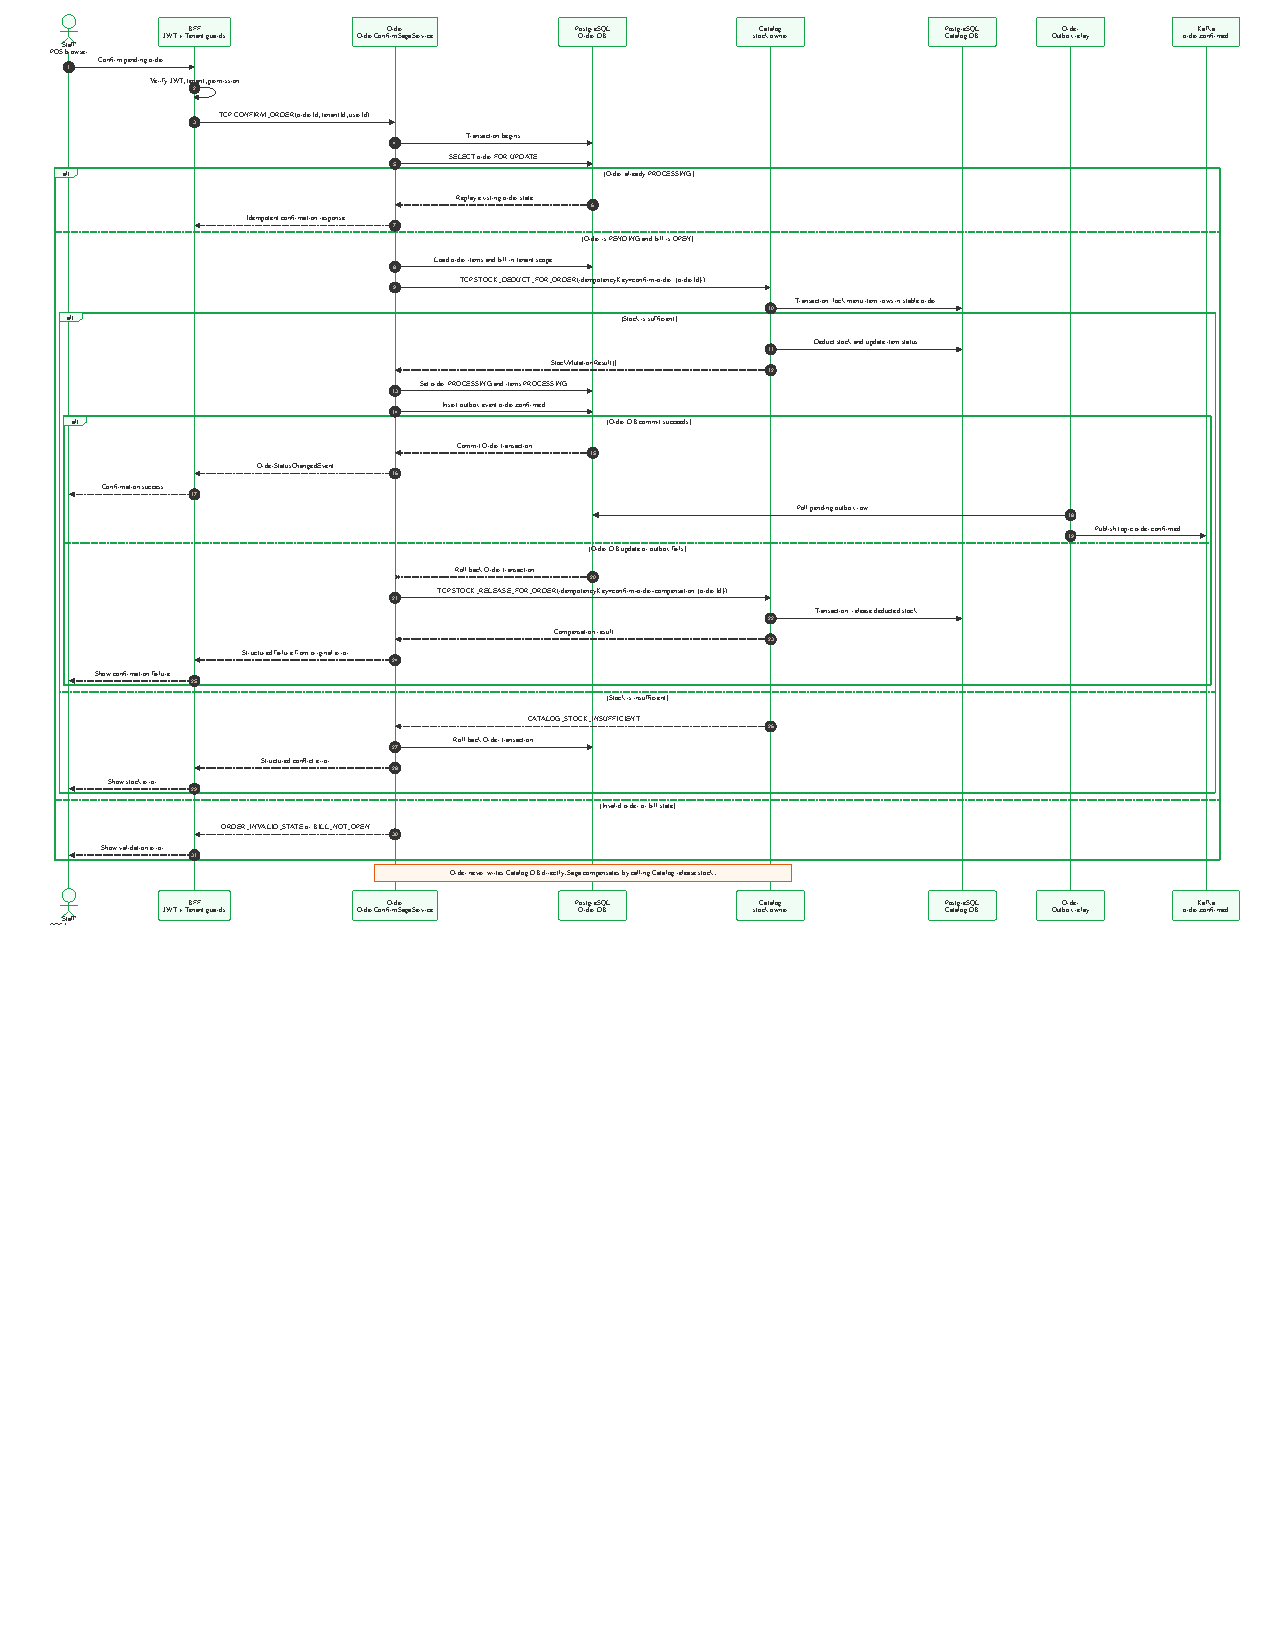
\includegraphics[width=\textwidth,height=0.82\textheight,keepaspectratio]{chapter5-order-confirm-stock.pdf}
  \caption{Order Confirm Saga: xác nhận đơn hàng và bảo toàn tồn kho qua ranh giới Order--Catalog.}
  \label{fig:chapter5-order-confirm-stock}
\end{figure}

Mục tiêu nghiệp vụ của luồng này là chỉ chuyển đơn sang trạng thái chế biến khi nhân viên đã xác nhận và tồn kho còn đủ. Bất biến cần giữ là Catalog là chủ sở hữu duy nhất của tồn kho, Order là chủ sở hữu vòng đời đơn/hóa đơn, và việc xác nhận lặp lại không được trừ tồn kho hai lần. Đây là Order Confirm Saga, Saga đại diện cho lõi POS của QRTable.

Khi nhân viên xác nhận đơn từ POS, BFF kiểm tra JWT, ngữ cảnh đơn vị thuê bao và quyền thao tác trước khi gọi Order. Order khóa đơn trong phạm vi đơn vị thuê bao, kiểm tra trạng thái đơn/hóa đơn, rồi gọi Catalog qua hợp đồng để trừ tồn kho. Catalog thực hiện phần cập nhật tồn kho trong cơ sở dữ liệu của chính Catalog. Nếu thiếu tồn kho, Order không được chuyển trạng thái đơn sang chế biến. Nếu Catalog trừ thành công nhưng bước cập nhật Order hoặc ghi outbox thất bại, Order gọi lại Catalog để bù trừ bằng đường hoàn tồn kho tương ứng.

Sau khi Order ghi nhận thành công, outbox \texttt{order.confirmed} trở thành bằng chứng của điểm ghi nhận nghiệp vụ và được thành phần xuất bản phát sang Kafka để Kitchen dựng phiếu bếp. Phản hồi cho nhân viên tách khỏi thời điểm Kitchen xử lý xong phiếu bếp, vì KDS là tác dụng phụ bất đồng bộ sau bước xác nhận. Trong phạm vi triển khai, Order Confirm Saga là luồng đại diện để chứng minh cách QRTable phối hợp transaction cục bộ, outbox event và compensation khi xác nhận đơn. Các cơ chế hardening như trạng thái Saga bền vững, CDC hoặc phân phối exactly-once thuộc hướng củng cố sau khi luồng đại diện đã chứng minh được giá trị kiến trúc.

Hình~\ref{fig:chapter5-screenshot-staff-table-map} và Hình~\ref{fig:chapter5-screenshot-staff-order-confirm} minh họa luồng thành công của Order Confirm Saga trên client POS (Hình~\ref{fig:chapter5-order-confirm-stock}): nhân viên xem sơ đồ bàn và đơn đang mở, rồi xác nhận đơn để kích hoạt trừ tồn kho qua Catalog. Nhánh bù trừ khi thất bại được chứng minh bằng kiểm thử tự động; kết quả kiểm thử được tổng hợp ở Chương~6 và hiện vật lưu ở Phụ lục~\ref{app:test-evidence}.

\screenshotfiguremgmt{chapter5-05-staff-pos-table-map.png}{Client POS — sơ đồ bàn (\texttt{/pos/tables}): nhân viên theo dõi trạng thái bàn, đơn và hóa đơn đang mở trước bước xác nhận trong Order Confirm Saga.}{fig:chapter5-screenshot-staff-table-map}
\screenshotfiguremgmt{chapter5-06-staff-order-confirm.png}{Client POS — xác nhận đơn: nhân viên chuyển đơn từ chờ xác nhận sang chế biến sau khi Order phối hợp Catalog kiểm tra và trừ tồn kho.}{fig:chapter5-screenshot-staff-order-confirm}

\section{Điều phối bếp/KDS và cập nhật thời gian thực}

Hình~\ref{fig:chapter5-kds-ticket-lifecycle} mô tả cách Kitchen nhận sự kiện \texttt{order.confirmed}, tạo phiếu KDS, phát gợi ý thời gian thực và để client lấy lại bản chụp trạng thái.

\begin{figure}[H]
  \centering
  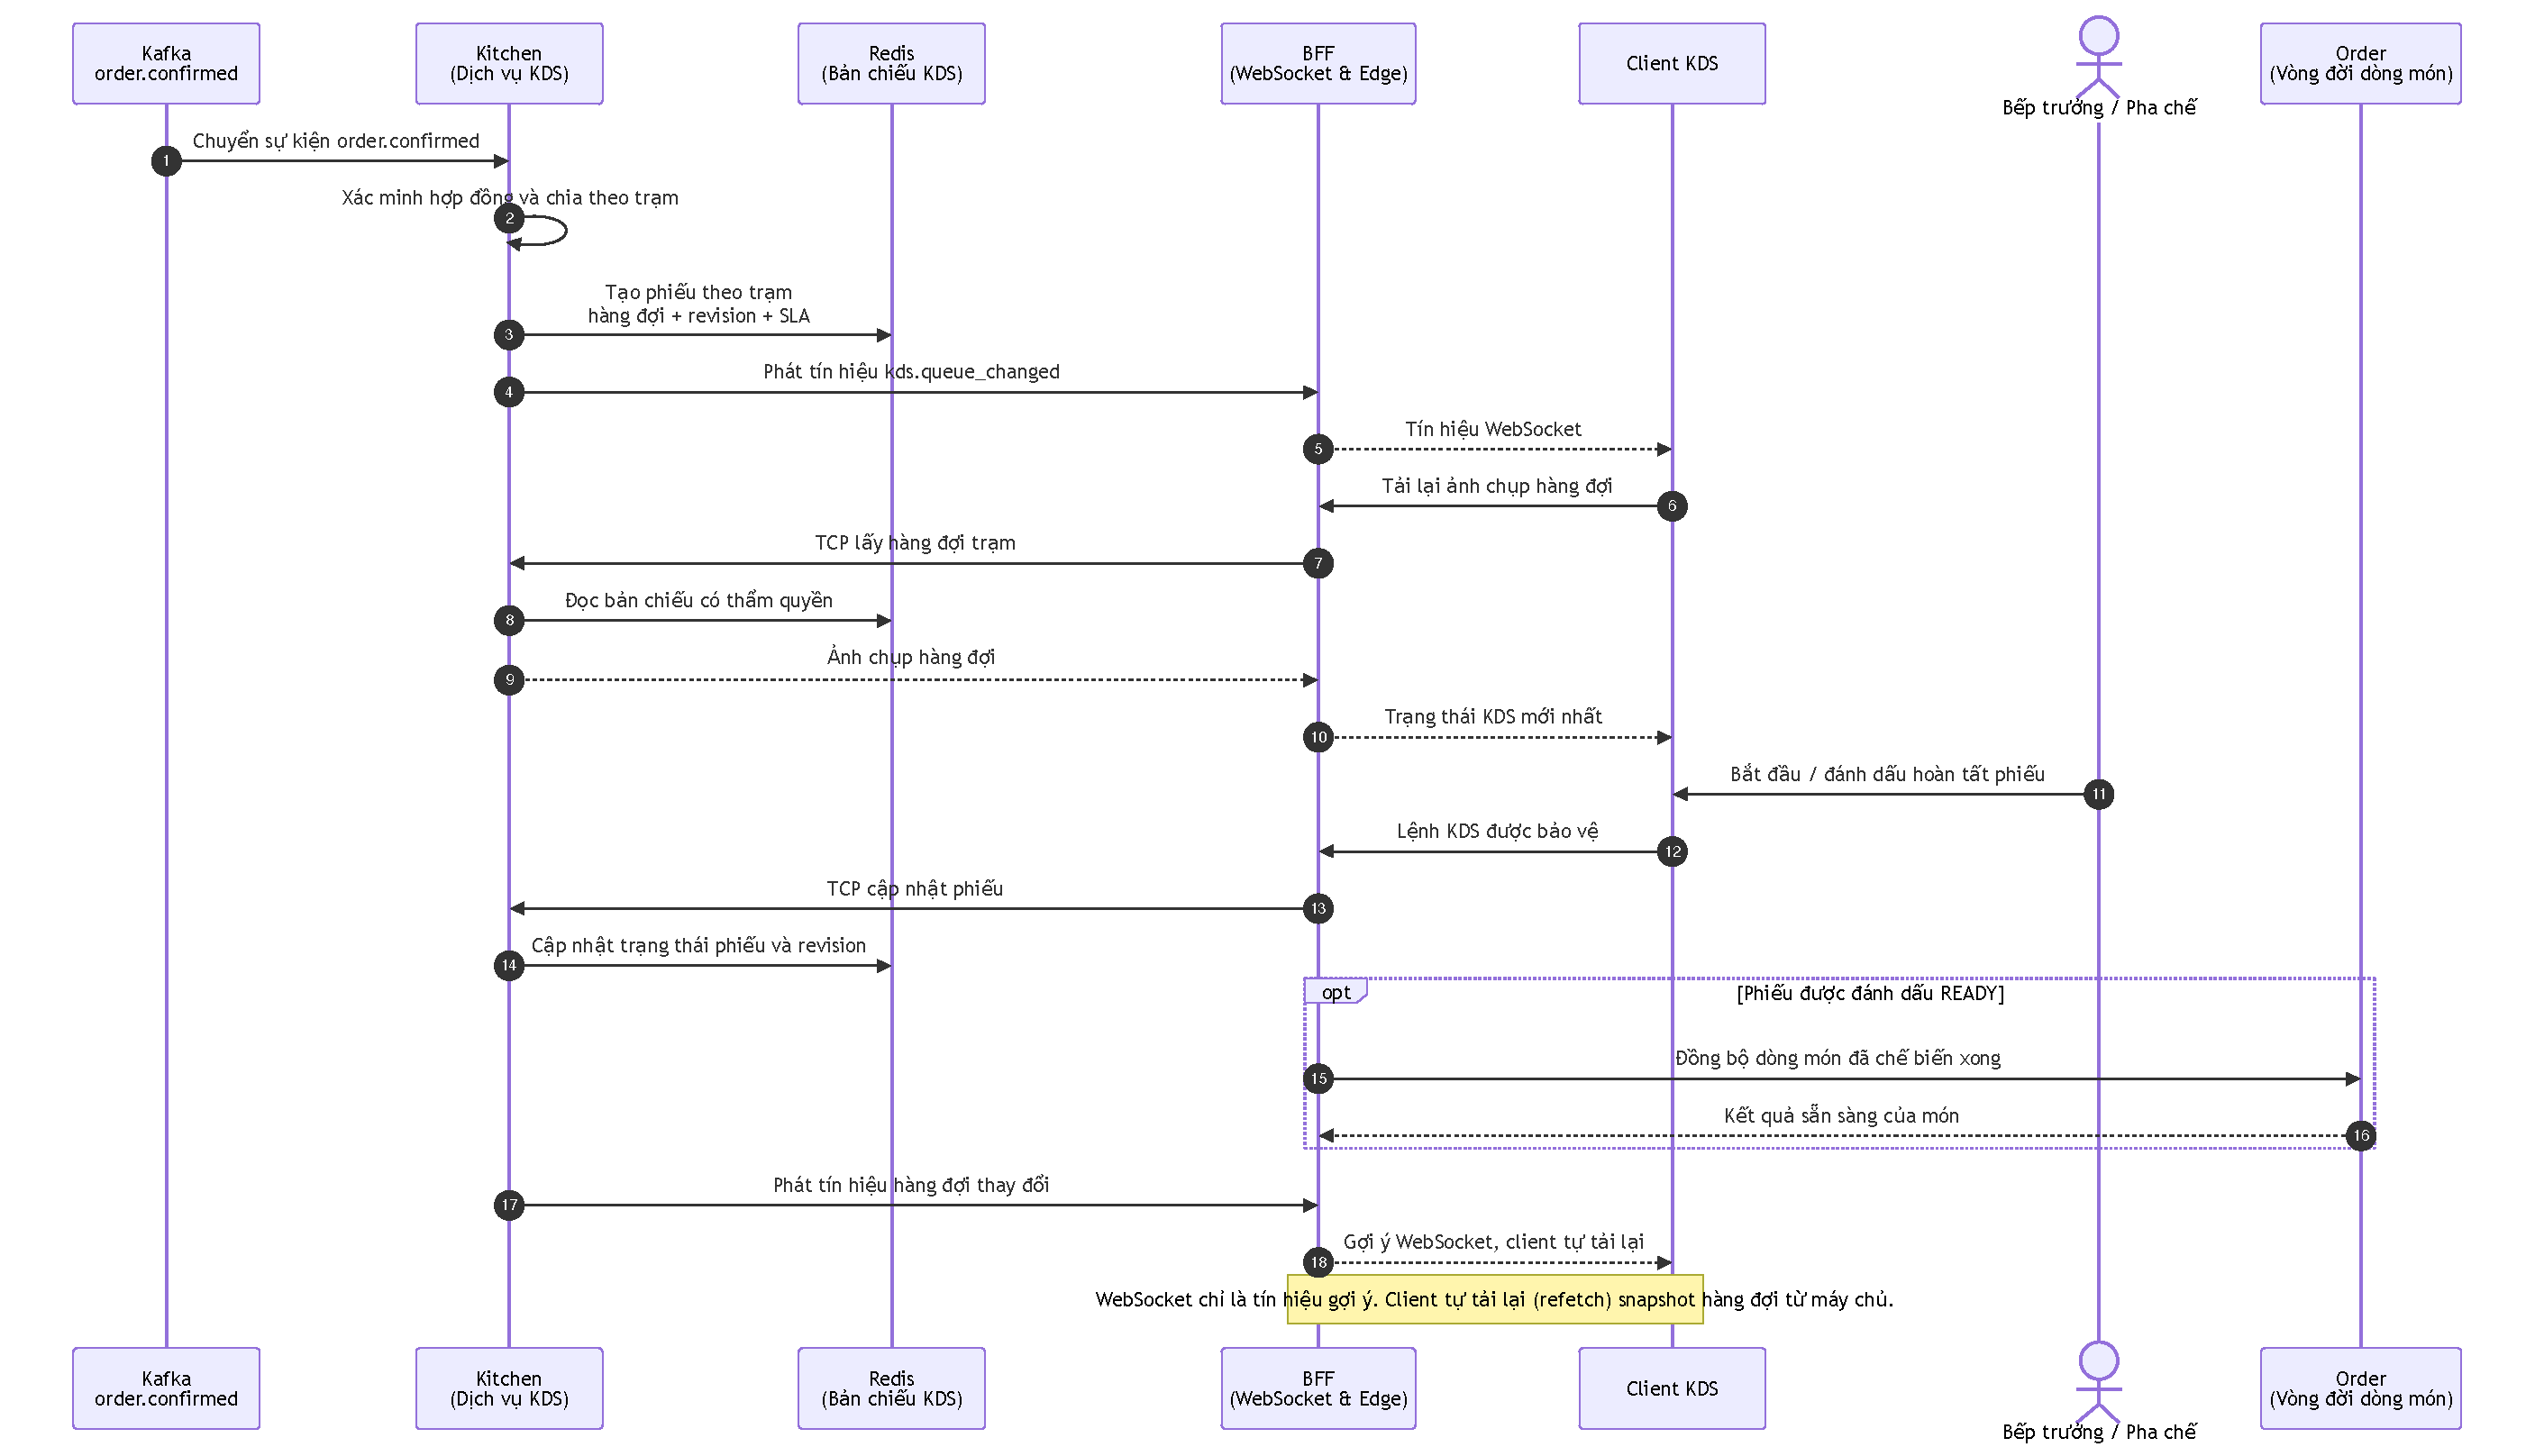
\includegraphics[width=\textwidth,height=0.82\textheight,keepaspectratio]{chapter5-kds-ticket-lifecycle.pdf}
  \caption{Luồng điều phối KDS từ sự kiện Order đến gợi ý WebSocket và tải lại dữ liệu.}
  \label{fig:chapter5-kds-ticket-lifecycle}
\end{figure}

Mục tiêu nghiệp vụ của luồng này là đưa món đã xác nhận đến đúng trạm bếp/bar, hỗ trợ cập nhật trạng thái phiếu bếp và phản ánh thay đổi cho màn hình KDS gần thời gian thực. Bất biến cần giữ là Kitchen sở hữu hàng đợi KDS khi vận hành, nhưng Order vẫn sở hữu vòng đời đơn và dòng đơn. Kitchen không có cơ sở dữ liệu nghiệp vụ bền vững riêng trong phạm vi hiện tại; Redis là bản chiếu khi vận hành để phục vụ hàng đợi, phiên bản, SLA và khôi phục.

Kitchen tiêu thụ chủ đề Kafka \texttt{order.confirmed}, kiểm tra nội dung sự kiện theo hợp đồng rồi tách phiếu bếp theo trạm. Phiếu được lưu trong Redis theo cấu trúc phù hợp với hàng đợi, ưu tiên và SLA. Sau mỗi thay đổi, Kitchen phát sự kiện \texttt{kds.queue\_changed} cho BFF qua kênh nội bộ; BFF gửi gợi ý WebSocket đến client KDS; client làm mới truy vấn và gọi lại API để lấy bản chụp trạng thái mới. Cách làm này giữ đúng nguyên tắc WebSocket là tín hiệu làm mới, còn trạng thái có thẩm quyền nằm ở phía máy chủ.

Khi đầu bếp bắt đầu hoặc hoàn tất phiếu bếp, thao tác đi qua BFF đến Kitchen. Nếu phiếu đã sẵn sàng làm thay đổi trạng thái dòng món, Kitchen phối hợp với Order qua hợp đồng để Order cập nhật vòng đời dòng món/đơn tương ứng. KDS trong Chương 5 được trình bày như bản chiếu vận hành gần thời gian thực cho bếp/bar. Lịch sử bếp dài hạn hoặc phân tích chuyên sâu phù hợp hơn với bản chiếu bền vững hoặc kho phân tích trong hướng phát triển.

Hình~\ref{fig:chapter5-screenshot-kds-queue} và Hình~\ref{fig:chapter5-screenshot-kds-ticket-status} minh họa client KDS (Hình~\ref{fig:chapter5-kds-ticket-lifecycle}): tiếp nhận phiếu sau sự kiện \texttt{order.confirmed} và cập nhật trạng thái phiếu trên hàng đợi khi vận hành.

\screenshotfiguremgmt{chapter5-07-kds-queue.png}{Client KDS — hàng đợi bếp/bar: phiếu món xuất hiện sau khi đơn được xác nhận, xếp theo trạm và ưu tiên trên bản chiếu Redis (Hình~\ref{fig:chapter5-kds-ticket-lifecycle}).}{fig:chapter5-screenshot-kds-queue}
\screenshotfiguremgmt{chapter5-08-kds-ticket-status.png}{Client KDS — cập nhật trạng thái phiếu (bắt đầu, sẵn sàng, bump); thay đổi được phát qua WebSocket gợi ý làm mới và client tải lại snapshot hàng đợi.}{fig:chapter5-screenshot-kds-ticket-status}

\section{Ghi nhận thanh toán tiền mặt, VietQR và SePay}

Hình~\ref{fig:chapter5-payment-settlement} gom hai nhánh thanh toán chính: tiền mặt tại POS và VietQR/SePay qua webhook.

\begin{figure}[H]
  \centering
  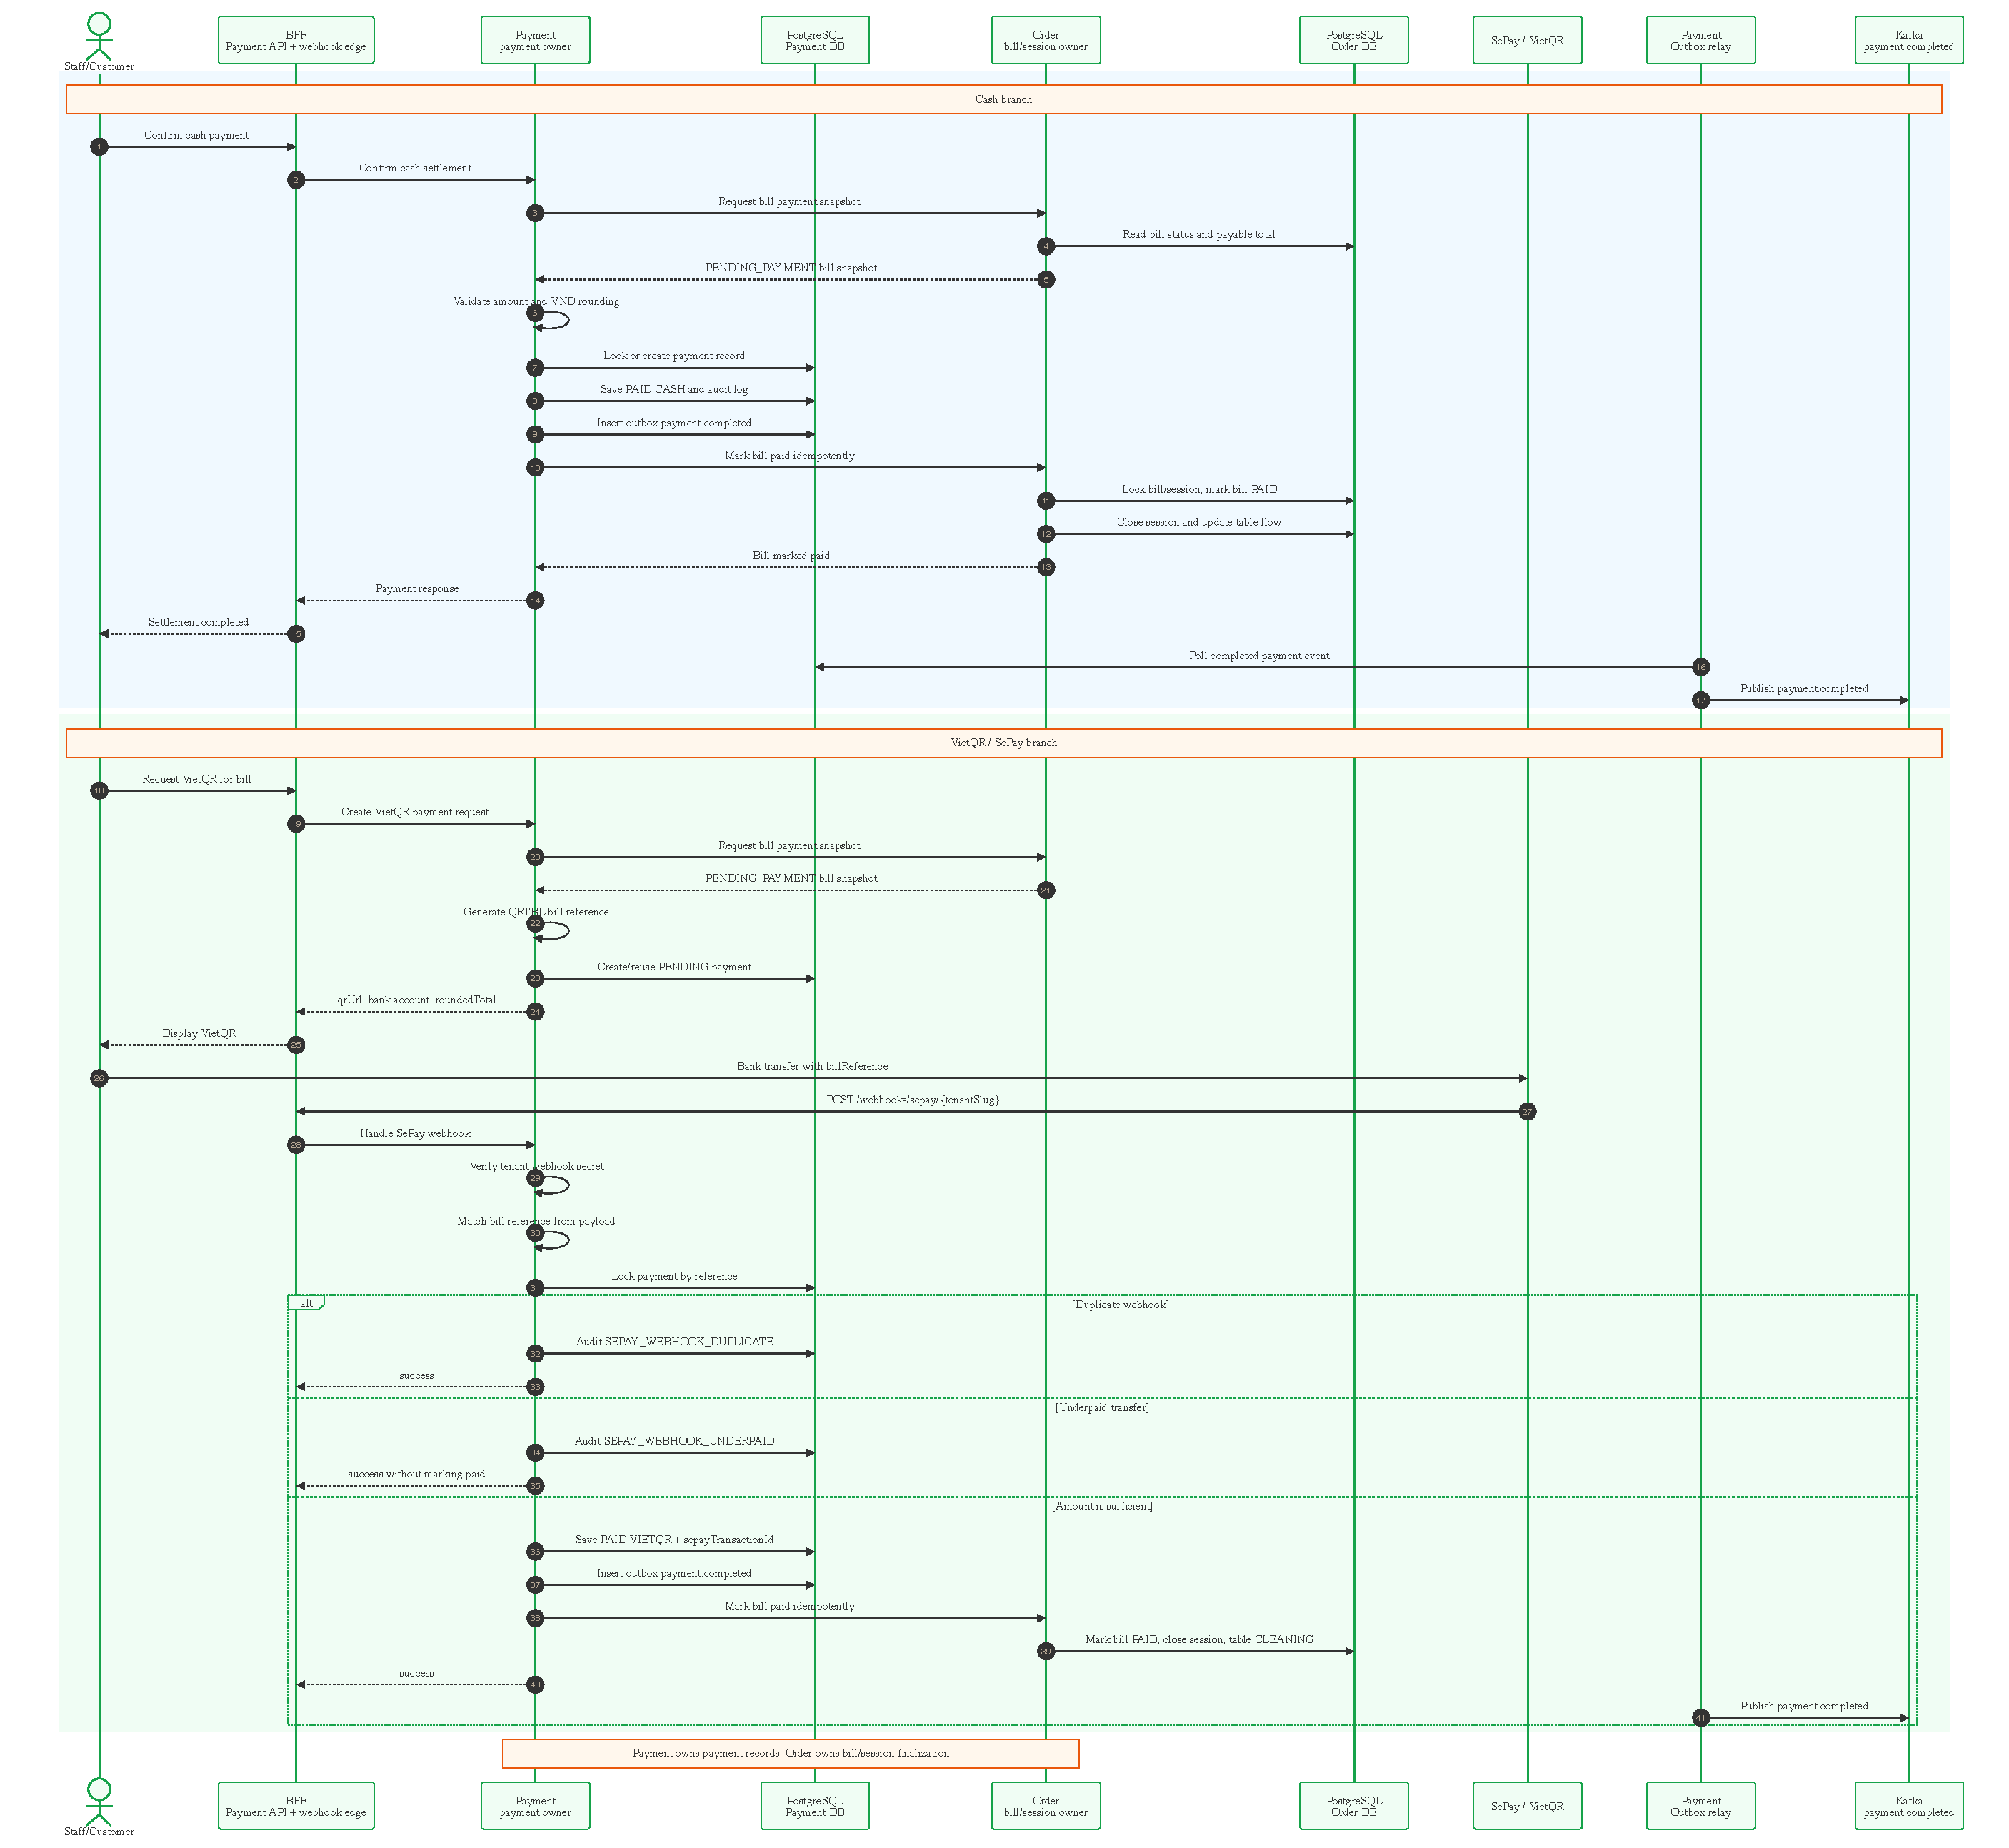
\includegraphics[width=\textwidth,height=0.82\textheight,keepaspectratio]{chapter5-payment-settlement.pdf}
  \caption{Luồng ghi nhận thanh toán tiền mặt, VietQR và SePay.}
  \label{fig:chapter5-payment-settlement}
\end{figure}

Mục tiêu nghiệp vụ của luồng này là ghi nhận thanh toán đúng hóa đơn, đúng đơn vị thuê bao, đúng số tiền đã làm tròn VND và không hoàn tất hóa đơn nhiều lần khi có yêu cầu hoặc webhook lặp. Bất biến dữ liệu là Payment sở hữu bản ghi thanh toán, nhật ký thanh toán, cấu hình thanh toán và outbox thanh toán; Order sở hữu việc hoàn tất hóa đơn/phiên; Catalog sở hữu trạng thái bàn sau khi phiên kết thúc.

Với tiền mặt, Payment lấy bản chụp hóa đơn từ Order qua hợp đồng, kiểm tra số tiền và ghi thanh toán, nhật ký kiểm toán và outbox trong cơ sở dữ liệu Payment. Sau đó Payment phối hợp với Order để đánh dấu hóa đơn đã thanh toán, đóng phiên, xóa trạng thái phiên/giỏ khi vận hành và chuyển bàn sang trạng thái phù hợp. Nếu cùng một giao dịch thanh toán được phát lại, phần hoàn tất hóa đơn phải đi theo hướng lũy đẳng để không tạo kết quả trùng.

Với VietQR/SePay, Payment tạo tham chiếu hóa đơn nhà hàng theo dòng tiền \texttt{QRTBL}. Webhook từ SePay đi vào BFF, được định tuyến và chuyển cho Payment. Payment kiểm tra bí mật của đơn vị thuê bao, khớp tham chiếu từ nội dung chuyển khoản, khóa bản ghi thanh toán, ghi nhật ký cho giao dịch trùng hoặc thanh toán thiếu, và chỉ gọi Order hoàn tất hóa đơn khi đủ điều kiện. Cấu hình tài khoản và trạng thái OAuth ngắn hạn thuộc Payment; hóa đơn gói nền tảng \texttt{QRSUB} thuộc SaaS, không bị trộn với bản ghi thanh toán của hóa đơn nhà hàng.

Phần triển khai thanh toán chứng minh đường cơ sở xử lý tiền mặt, webhook VietQR/SePay, webhook trùng và thanh toán thiếu bằng mã nguồn/kiểm thử nội bộ. Môi trường production được triển khai để thu đường gọi lại public, thông tin xác thực hợp lệ và dữ liệu giao dịch thật; nhóm hiện vật này giúp Chương 6 phân biệt kết luận dựa trên kiểm thử nội bộ với kết luận provider live.

Hình~\ref{fig:chapter5-screenshot-customer-payment-flow} minh họa nhánh khách của luồng thanh toán (Hình~\ref{fig:chapter5-payment-settlement}): theo dõi tiến độ đơn và yêu cầu thanh toán VietQR tại bàn. Chương~6 đối chiếu thêm webhook SePay và tính lũy đẳng ghi nhận thanh toán với kiểm thử tương ứng.

\screenshotpwafiguretwo{Customer PWA — nhánh thanh toán phía khách (Hình~\ref{fig:chapter5-payment-settlement}): trái, màn theo dõi đơn (\texttt{/order-tracking}) sau khi gửi món; phải, yêu cầu thanh toán và hiển thị VietQR (\texttt{/request-payment}).}{fig:chapter5-screenshot-customer-payment-flow}{chapter5-04-customer-order-tracking.png}{chapter5-04-customer-request-payment.png}
\screenshotgridanchor{fig:chapter5-screenshot-customer-order-tracking}
\screenshotgridanchor{fig:chapter5-screenshot-customer-request-payment}

\section{Khởi tạo đơn vị thuê bao và vòng đời gói dịch vụ}

Hình~\ref{fig:chapter5-saas-onboarding-saga} trình bày luồng Super Admin khởi tạo đơn vị thuê bao và các tác dụng phụ cần bù trừ khi một bước phụ thuộc thất bại.

\begin{figure}[H]
  \centering
  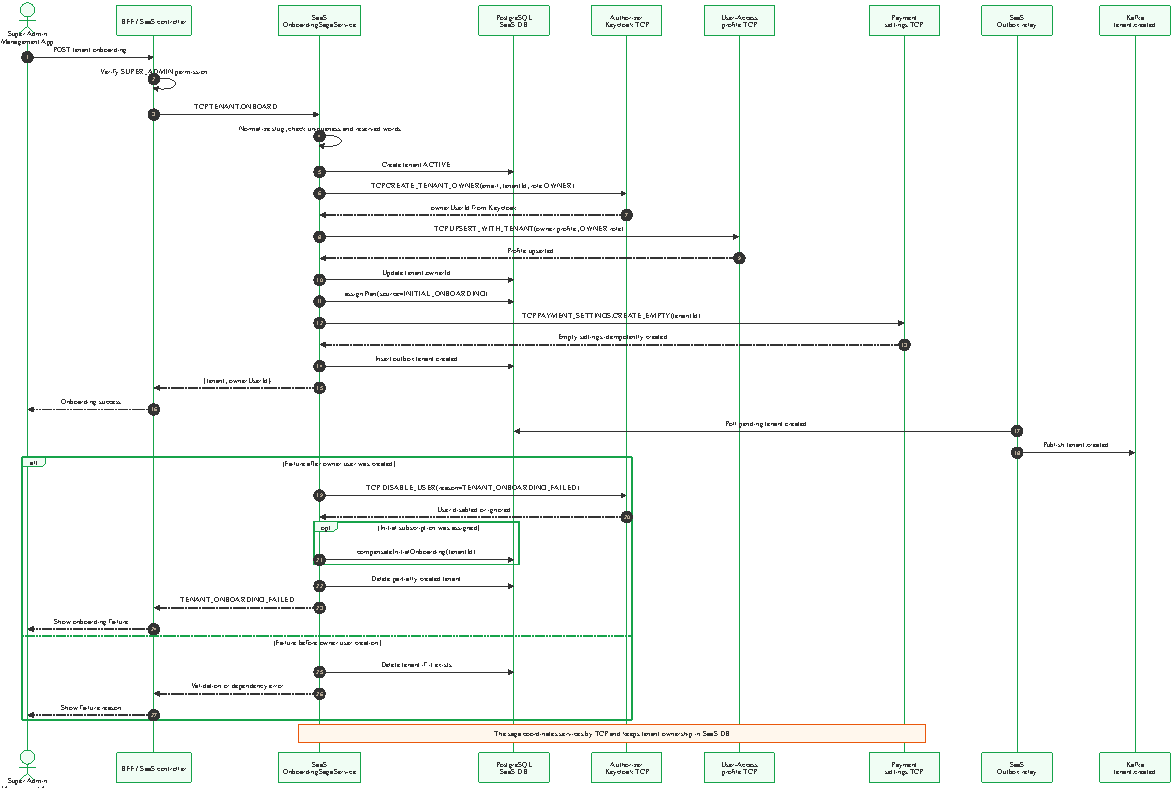
\includegraphics[width=\textwidth,height=0.82\textheight,keepaspectratio]{chapter5-saas-onboarding-saga.pdf}
  \caption{Luồng khởi tạo đơn vị thuê bao theo SaaS Onboarding Mini-Saga.}
  \label{fig:chapter5-saas-onboarding-saga}
\end{figure}

Mục tiêu nghiệp vụ của luồng này là tạo một đơn vị thuê bao có thể vận hành: có thông tin đơn vị thuê bao, chủ sở hữu, hồ sơ/vai trò, gói thuê bao ban đầu và cấu hình thanh toán tương ứng. Bất biến cần giữ là SaaS sở hữu đơn vị thuê bao, gói, thuê bao và hóa đơn thuê bao; Authorizer/Keycloak sở hữu định danh; User-Access sở hữu hồ sơ ứng dụng và vai trò; Payment sở hữu cấu hình thanh toán. SaaS không tự ghi dữ liệu của User-Access hoặc Payment.

Luồng bắt đầu từ Super Admin trong Management App. BFF kiểm tra quyền quản trị nền tảng trước khi gọi SaaS. SaaS chuẩn hóa slug, kiểm tra trùng lặp và tạo đơn vị thuê bao cùng thuê bao gói trong cơ sở dữ liệu của SaaS. Sau đó, SaaS gọi Authorizer để tạo định danh chủ sở hữu, gọi User-Access để tạo hồ sơ và vai trò ứng dụng, gọi Payment để tạo cấu hình thanh toán rỗng, rồi ghi outbox \texttt{tenant.created}. Nếu lỗi xảy ra sau khi đã có tác dụng phụ, SaaS thực hiện bù trừ như vô hiệu hóa chủ sở hữu đã tạo, hủy thuê bao khởi tạo hoặc xóa đơn vị thuê bao chưa hoàn tất.

Vòng đời đơn vị thuê bao sau khi khởi tạo gồm hoạt động, tạm ngưng và đóng. SaaS giữ trạng thái bền vững, Redis hỗ trợ đường đọc nhanh cho guard và quyền theo gói thuê bao. Khi đơn vị thuê bao bị tạm ngưng, hệ thống cần phân biệt các thao tác còn được phép, chẳng hạn đọc một số thông tin hoặc xử lý thanh toán đang chờ, với các thao tác tạo đơn mới hoặc thay đổi dữ liệu không phù hợp. Đây là Saga đại diện thứ hai của đề tài; giống luồng xác nhận đơn, chương này dùng mini-saga để chứng minh orchestration và compensation có kiểm soát, còn tiến trình thử lại độc lập hoặc trạng thái Saga bền vững là hướng củng cố sau phạm vi luồng đại diện.

Hình~\ref{fig:chapter5-screenshot-admin-tenant-onboarding}, Hình~\ref{fig:chapter5-screenshot-owner-payment-settings} và Hình~\ref{fig:chapter5-screenshot-owner-subscription} minh họa các bước sau SaaS Onboarding Mini-Saga (Hình~\ref{fig:chapter5-saas-onboarding-saga}): Super Admin tạo đơn vị thuê bao, chủ quán cấu hình kênh thanh toán và xem gói thuê bao đang hoạt động. Chương~6 và Phụ lục~\ref{app:test-evidence} đối chiếu phần điều phối và bù trừ của mini-saga với kiểm thử tương ứng.

\screenshotfiguremgmt{chapter5-12-admin-tenant-onboarding.png}{Management App — Super Admin khởi tạo đơn vị thuê bao, chủ sở hữu và gói ban đầu; điểm bắt đầu SaaS Onboarding Mini-Saga (Hình~\ref{fig:chapter5-saas-onboarding-saga}).}{fig:chapter5-screenshot-admin-tenant-onboarding}
\screenshotfiguremgmt{chapter5-11-owner-payment-settings.png}{Management App — Owner cấu hình thanh toán (\texttt{/dashboard/payment-settings}): liên kết SePay/VietQR và tham số ghi nhận thanh toán cho đơn vị thuê bao sau onboarding.}{fig:chapter5-screenshot-owner-payment-settings}
\screenshotfiguremgmt{chapter5-11-owner-subscription.png}{Management App — Owner xem gói thuê bao và trạng thái đăng ký (\texttt{/dashboard/subscription}), căn cứ cho guard quyền theo gói khi vận hành.}{fig:chapter5-screenshot-owner-subscription}

\section{Bảng điều khiển và báo cáo theo gói dịch vụ}

Phần bảng điều khiển và báo cáo bổ sung lớp đọc tổng hợp cho QRTable mà không tạo thêm một dịch vụ phân tích độc lập. Mục tiêu nghiệp vụ là cho Owner/Manager thấy tình hình vận hành của đơn vị thuê bao như doanh thu, đơn hàng, phương thức thanh toán, món bán chạy và trạng thái bàn; đồng thời cho Super Admin thấy số liệu nền tảng như đơn vị thuê bao, thuê bao gói, hóa đơn và doanh thu gói dịch vụ.

Về ranh giới dữ liệu, BFF là lớp HTTP được bảo vệ bằng guard. BFF kiểm tra quyền \texttt{report.read\_own} hoặc \texttt{report.read\_any}, chuẩn hóa truy vấn và chuyển yêu cầu đến dịch vụ sở hữu dữ liệu. Payment cung cấp số liệu doanh thu và phương thức thanh toán; Order cung cấp số liệu đơn/hóa đơn/món bán chạy; Catalog cung cấp trạng thái bàn/thực đơn; SaaS cung cấp số liệu nền tảng. Cách làm này giữ nguyên quyền sở hữu dữ liệu đã trình bày ở Chương 4; các đường xử lý phân tích Kafka hoặc kho OLAP thuộc nhóm mở rộng phân tích.

Điểm khác biệt giữa bảng điều khiển theo đơn vị thuê bao và phân tích nền tảng nằm ở quyền theo gói. Owner/Manager dùng \texttt{report.read\_own} và API báo cáo theo đơn vị thuê bao còn bị kiểm tra thuê bao đang hoạt động cùng tính năng \texttt{analytics\_basic}; client hiển thị trạng thái khóa hoặc mở theo gói. Super Admin dùng \texttt{report.read\_any} cho phân tích nền tảng và thao tác khoan sâu theo đơn vị thuê bao, không bị khóa bởi gói của đơn vị thuê bao đang được xem. Dashboard/reporting trong Chương 5 được chứng minh bằng mô hình đọc vận hành và entitlement theo gói. Các năng lực phân tích nâng cao như forecasting, phân tích hiệu suất nhân viên, kênh doanh thu thời gian thực hoặc kho dữ liệu phân tích được giữ cho hướng phát triển.

Hình~\ref{fig:chapter5-screenshot-owner-menu-management} và Hình~\ref{fig:chapter5-screenshot-owner-table-qr} minh họa Owner thiết lập dữ liệu nền (thực đơn, bàn, mã QR) trước khi khách quét QR. Hình~\ref{fig:chapter5-screenshot-owner-dashboard-reporting} và Hình~\ref{fig:chapter5-screenshot-admin-platform-analytics} minh họa mô hình đọc báo cáo theo quyền \texttt{report.read\_own} và \texttt{report.read\_any}.

\screenshotfiguremgmt{chapter5-09-owner-menu-management.png}{Management App — Owner quản trị thực đơn (\texttt{/dashboard/menu}): danh mục, món và tồn kho thuộc phạm vi Catalog là nguồn sự thật cho luồng đặt món.}{fig:chapter5-screenshot-owner-menu-management}
\screenshotfiguremgmt{chapter5-10-owner-table-qr-management.png}{Management App — Owner quản lý khu vực, bàn và mã QR (\texttt{/dashboard/tables}): mã QR gắn bàn là điểm vào phiên Customer PWA.}{fig:chapter5-screenshot-owner-table-qr}
\screenshotfiguremgmt{chapter5-13-owner-dashboard-reporting.png}{Management App — bảng điều khiển Owner/Manager (\texttt{/dashboard}): tổng hợp doanh thu và đơn hàng khi gói có entitlement \texttt{analytics\_basic}.}{fig:chapter5-screenshot-owner-dashboard-reporting}
\screenshotfiguremgmt{chapter5-14-admin-platform-analytics.png}{Management App — Super Admin phân tích nền tảng (\texttt{/admin/analytics}): số liệu đơn vị thuê bao, thuê bao gói và doanh thu SaaS theo quyền \texttt{report.read\_any}.}{fig:chapter5-screenshot-admin-platform-analytics}

\section{Đóng gói triển khai và khung minh chứng production}

QRTable có nền tảng đóng gói bằng Docker/Docker Compose và các thành phần phụ thuộc như PostgreSQL, MongoDB, Redis, Kafka, Keycloak, BFF và các ứng dụng phía người dùng. Phần đóng gói triển khai là cầu nối trực tiếp sang lớp minh chứng production, nơi hệ thống được chạy với URL hoặc tên miền công khai, HTTPS/TLS theo cấu hình môi trường, cấu hình BFF và ứng dụng phía người dùng, kết nối PostgreSQL, Redis, Kafka và Keycloak, đường gọi lại webhook SePay công khai, kiểm tra sức khỏe/sẵn sàng và kiểm thử khói các luồng phiên QR, xác nhận đơn, KDS, thanh toán và khởi tạo đơn vị thuê bao.

Các hiện vật production như ảnh kiểm tra sức khỏe, nhật ký rút gọn, kết quả kiểm thử khói, cấu hình đường gọi lại công khai, phiên bản/phát hành/mã commit và danh sách kiểm tra hoàn tác cơ bản được dùng để củng cố kết luận về khả năng đóng gói và vận hành các dịch vụ chính trên môi trường production. Các thuộc tính như tính sẵn sàng cao, tự động hoàn tác hoặc kiểm thử tải thuộc nhóm hiện vật riêng trước khi trở thành kết quả đánh giá chính.

\section{Tổng hợp minh chứng triển khai}

Bảng~\ref{tab:chapter5-implemented-evidence} tóm tắt các luồng chính theo mục tiêu, bất biến, bằng chứng và ranh giới đánh giá. Bảng này thay thế cách liệt kê cây mã nguồn hoặc thư viện dùng chung dài; mỗi dòng chỉ giữ thông tin cần thiết để người đọc thấy luồng đã được hiện thực và vẫn còn ranh giới đánh giá rõ ràng.

{\scriptsize\sloppy
\setlength{\tabcolsep}{2pt}
\begin{longtable}{>{\raggedright\arraybackslash}p{0.16\textwidth}>{\raggedright\arraybackslash}p{0.24\textwidth}>{\raggedright\arraybackslash}p{0.25\textwidth}>{\raggedright\arraybackslash}p{0.17\textwidth}>{\raggedright\arraybackslash}p{0.1\textwidth}}
  \caption{Tổng hợp minh chứng triển khai các luồng cốt lõi của QRTable.}
  \label{tab:chapter5-implemented-evidence}\\
  \toprule
  Luồng & Mục tiêu nghiệp vụ & Bất biến / ranh giới chính & Bằng chứng chính & Ranh giới đánh giá \\
  \midrule
  \endfirsthead
  \toprule
  Luồng & Mục tiêu nghiệp vụ & Bất biến / ranh giới chính & Bằng chứng chính & Ranh giới đánh giá \\
  \midrule
  \endhead
  \bottomrule
  \endfoot
  Phiên QR và giỏ chung & Khách vào phiên từ QR, dùng chung giỏ và gửi đơn. & Order sở hữu phiên/giỏ/đơn; Catalog sở hữu bàn/thực đơn; Redis chỉ hỗ trợ đường xử lý nóng. & Hình~\ref{fig:chapter5-qr-ordering-session}; kiểm thử phiên/giỏ/gửi đơn của Order. & Tập trung vào phiên trực tuyến, kết nối lại và tải lại snapshot; offline queue đầy đủ là hướng mở rộng. \\
  Xác nhận đơn và tồn kho & Nhân viên xác nhận đơn khi đủ tồn kho. & Catalog là chủ tồn kho; Order là chủ đơn; xác nhận lặp không trừ tồn kho lần hai. & Hình~\ref{fig:chapter5-order-confirm-stock}; kiểm thử đơn vị và kiểm thử hợp đồng cho Order Confirm Saga; kiểm thử tích hợp tồn kho có điều kiện. & Chứng minh Saga đại diện; hardening như durable saga state, CDC hoặc exactly-once là hướng củng cố. \\
  KDS & Phiếu bếp/bar xuất hiện sau khi đơn được xác nhận và client cập nhật gần thời gian thực. & Kitchen sở hữu bản chiếu Redis; Order vẫn sở hữu vòng đời đơn/dòng đơn; WebSocket là gợi ý/tải lại. & Hình~\ref{fig:chapter5-kds-ticket-lifecycle}; kiểm thử bộ tiêu thụ Kitchen/KDS. & Bản chiếu phục vụ vận hành gần thời gian thực; lịch sử KDS dài hạn cần kho/bản chiếu bền vững riêng. \\
  Thanh toán & Ghi nhận tiền mặt hoặc VietQR/SePay và hoàn tất hóa đơn/phiên. & Payment sở hữu bản ghi thanh toán; Order sở hữu hóa đơn/phiên; webhook trùng/thiếu phải lũy đẳng. & Hình~\ref{fig:chapter5-payment-settlement}; kiểm thử ghi nhận thanh toán/webhook. & Kiểm thử nội bộ chứng minh idempotency; provider live gắn với hiện vật callback và dữ liệu giao dịch thật. \\
  Khởi tạo SaaS & Tạo đơn vị thuê bao, chủ sở hữu, thuê bao và cấu hình thanh toán. & SaaS sở hữu đơn vị thuê bao/thuê bao; Authorizer/User-Access/Payment chỉ qua hợp đồng; có bù trừ. & Hình~\ref{fig:chapter5-saas-onboarding-saga}; kiểm thử khởi tạo với cơ sở dữ liệu/Payment có điều kiện. & Chứng minh mini-saga đại diện; kiểm chứng đầu-cuối qua mọi phụ thuộc thuộc nhóm hiện vật toàn ngăn xếp. \\
  Bảng điều khiển/báo cáo & Owner/Manager và Super Admin xem báo cáo đúng quyền/gói. & BFF không truy vấn kết hợp trực tiếp cơ sở dữ liệu; Payment/Order/Catalog/SaaS giữ mô hình đọc của dữ liệu mình sở hữu. & Controller báo cáo BFF; dịch vụ báo cáo; kiểm thử báo cáo Management App. & Mô hình đọc vận hành và entitlement; phân tích nâng cao/kho dữ liệu thuộc hướng mở rộng. \\
  Đóng gói/triển khai production & Có khung kiểm chứng môi trường production. & Kết luận dựa trên URL, kiểm tra sức khỏe, kiểm thử khói và đường gọi lại webhook thật từ hiện vật production. & Docker, compose và cấu hình hiện có; khung kiểm chứng triển khai production. & Củng cố khả năng đóng gói và vận hành trên môi trường production; high availability hoặc rollback tự động cần bằng chứng riêng. \\
\end{longtable}
}

Bảng~\ref{tab:chapter5-representative-sagas} đặt riêng hai Saga đại diện cạnh nhau để tránh nhầm lẫn giữa luồng Saga chính của POS và mini-saga cấp phát nền tảng. Cả hai đều dùng orchestration, contract giữa dịch vụ và compensation có kiểm soát; tuy nhiên loại bằng chứng và ranh giới đánh giá không giống nhau.

{\scriptsize\sloppy
\setlength{\tabcolsep}{2pt}
\begin{longtable}{>{\raggedright\arraybackslash}p{0.16\textwidth}>{\raggedright\arraybackslash}p{0.19\textwidth}>{\raggedright\arraybackslash}p{0.22\textwidth}>{\raggedright\arraybackslash}p{0.22\textwidth}>{\raggedright\arraybackslash}p{0.13\textwidth}}
  \caption{Hai Saga đại diện trong QRTable.}
  \label{tab:chapter5-representative-sagas}\\
  \toprule
  Saga & Mục tiêu & Thành phần tham gia & Điểm commit và compensation & Loại bằng chứng \\
  \midrule
  \endfirsthead
  \toprule
  Saga & Mục tiêu & Thành phần tham gia & Điểm commit và compensation & Loại bằng chứng \\
  \midrule
  \endhead
  \bottomrule
  \endfoot
  Order Confirm Saga & Xác nhận đơn tại POS và bảo toàn tồn kho. & BFF, Order, Catalog, Order outbox, Kafka và Kitchen. & Commit khi Order ghi trạng thái \texttt{PROCESSING} cùng outbox \texttt{order.confirmed}; nếu Catalog đã trừ tồn kho nhưng Order commit/outbox thất bại, Order gọi Catalog hoàn tồn kho. & Có bằng chứng tốt từ kiểm thử đơn vị và kiểm thử hợp đồng; tích hợp tồn kho có điều kiện; tiêm lỗi toàn ngăn xếp là hướng củng cố. \\
  SaaS Onboarding Mini-Saga & Khởi tạo đơn vị thuê bao có chủ sở hữu, gói ban đầu và cấu hình thanh toán. & BFF, SaaS, Authorizer và Keycloak, User-Access, Payment, SaaS outbox, Catalog consumer. & Commit khi SaaS tạo tenant/subscription, tạo cấu hình thanh toán và ghi outbox \texttt{tenant.created}; nếu lỗi sau tác dụng phụ, SaaS bù trừ tenant/subscription và vô hiệu hóa chủ sở hữu khi cần. & Tích hợp cơ sở dữ liệu và lát cắt Payment TCP có bằng chứng tốt; Authorizer, Keycloak và User-Access có bằng chứng một phần. \\
\end{longtable}
}

Từ các luồng trên, QRTable đã vượt khỏi bản mô tả kiến trúc để có hiện thực tương ứng ở các ngữ cảnh nghiệp vụ chính. Các luồng liên dịch vụ đi qua hợp đồng thay vì truy cập chéo cơ sở dữ liệu, và những bất biến quan trọng như cô lập đơn vị thuê bao, quyền sở hữu tồn kho, tính lũy đẳng thanh toán, bù trừ Saga và WebSocket gợi ý/tải lại đã được thể hiện trong mã nguồn, kiểm thử và sơ đồ. Chương 6 dùng các bằng chứng này để phân loại kết luận đã được kiểm chứng tự động, kết luận được hỗ trợ bởi thiết kế và kết luận được củng cố bằng hiện vật triển khai production.

\chapter{Kiểm chứng và đánh giá hệ thống QRTable}
\label{chap:danh-gia}

\newcommand{\chapterSixEvidenceFigure}[5][]{%
  \begin{figure}[htbp]%
    \centering%
    \includegraphics[width=\textwidth,height=#2,keepaspectratio]{#3}%
    \if\relax\detokenize{#1}\relax%
      \caption{#5}%
    \else%
      \caption[#1]{#5}%
    \fi%
    \label{#4}%
  \end{figure}%
}

\newcommand{\chapterSixEvidencePair}[8][]{%
  \begin{figure}[htbp]%
    \centering%
    \begin{minipage}[t]{0.49\textwidth}%
      \centering%
      \includegraphics[width=\linewidth,height=#2,keepaspectratio]{#3}%
    \end{minipage}\hfill%
    \begin{minipage}[t]{0.49\textwidth}%
      \centering%
      \includegraphics[width=\linewidth,height=#2,keepaspectratio]{#4}%
    \end{minipage}%
    \if\relax\detokenize{#1}\relax%
      \caption{#6}%
    \else%
      \caption[#1]{#6}%
    \fi%
    \label{#5}%
    \label{#7}%
    \label{#8}%
  \end{figure}%
}

Chương này đánh giá QRTable dựa trên mối liên hệ giữa yêu cầu, thiết kế, phần triển khai và kết quả kiểm chứng. Trọng tâm không phải là liệt kê từng màn hình hay từng đoạn mã, mà là phân tích ba nội dung chính: mức độ vận hành đúng của các luồng nghiệp vụ quan trọng trong phạm vi kiểm thử; khả năng giữ ranh giới dữ liệu và trách nhiệm dịch vụ của kiến trúc microservices; và phạm vi kết luận cần được giới hạn vì chưa có đủ điều kiện kiểm chứng.

Do QRTable là hệ thống phân tán, một kết quả kiểm thử đơn lẻ không đủ để kết luận toàn bộ hệ thống. Vì vậy, chương này kết hợp nhiều loại cơ sở đánh giá: kết quả kiểm thử tự động, hình minh họa từ luồng nghiệp vụ đại diện, trạng thái quan sát được trên công cụ vận hành và phân tích giới hạn. Cách kết hợp bằng chứng này tách rõ phần đã được kiểm chứng với phần chưa đủ điều kiện để mở rộng kết luận.

Cơ sở đối chiếu trực tiếp của chương là các nội dung đã trình bày ở Chương 4 và Chương 5: quyền sở hữu dữ liệu, giao tiếp liên dịch vụ, mô hình phân quyền, các luồng triển khai và bảng tổng hợp kết quả triển khai. Chương này không lặp lại toàn bộ thiết kế, mà tập trung vào mức độ các thiết kế đó được kiểm chứng qua kiểm thử và kết quả quan sát được.

\section{Phương pháp đánh giá và phân loại cơ sở kết luận}

Phương pháp đánh giá được tổ chức theo các lớp bằng chứng khác nhau. Lớp thứ nhất là kiểm thử tự động ở mức dịch vụ và luồng nghiệp vụ. Lớp thứ hai là quan sát trực tiếp trên các công cụ như Allure, Kafka, Redis, Docker và Vercel. Lớp thứ ba là phân tích kiến trúc dựa trên ranh giới dịch vụ, quyền sở hữu dữ liệu và cách các thành phần phối hợp với nhau. Lớp cuối cùng là phân tích giới hạn, nhằm tránh biến kết quả kiểm thử đại diện thành những kết luận vượt quá phạm vi của đề tài.

Việc phân lớp bằng chứng tạo cơ sở cho kết luận thận trọng hơn. Ví dụ, một luồng Playwright đạt trạng thái thành công cho thấy hệ thống xử lý được kịch bản QR--POS--KDS đại diện, nhưng chưa thay thế kiểm thử toàn bộ phạm vi API hoặc kiểm thử tải diện rộng. Tương tự, hình minh họa Kafka hoặc Redis phản ánh trạng thái trong một luồng cụ thể, nhưng không phải bằng chứng cho mọi trường hợp vận hành dài hạn.

{\footnotesize\sloppy
\setlength{\tabcolsep}{3pt}
\begin{longtable}{>{\raggedright\arraybackslash}p{0.17\textwidth}>{\raggedright\arraybackslash}p{0.31\textwidth}>{\raggedright\arraybackslash}p{0.28\textwidth}>{\raggedright\arraybackslash}p{0.16\textwidth}}
  \caption{Nguyên tắc phân loại kết luận theo cơ sở đánh giá.}
  \label{tab:chapter6-evidence-policy}\\
  \toprule
  Mức kết luận & Cơ sở đánh giá & Phạm vi kết luận & Ví dụ trong QRTable \\
  \midrule
  \endfirsthead
  \toprule
  Mức kết luận & Cơ sở đánh giá & Phạm vi kết luận & Ví dụ trong QRTable \\
  \midrule
  \endhead
  \bottomrule
  \endfoot
  A -- Kiểm chứng tự động & Kiểm thử chạy thành công theo kịch bản xác định. & Kết luận trong phạm vi kịch bản kiểm thử. & Gửi đơn, thanh toán, KDS, Saga đại diện. \\
  B -- Quan sát bằng công cụ & Hình minh họa hoặc báo cáo từ công cụ trong một lần chạy cụ thể. & Cho thấy trạng thái đã được quan sát, không thay thế kiểm thử hồi quy. & Allure, Kafka, Redis, Docker, Vercel. \\
  C -- Hỗ trợ bởi thiết kế & Sơ đồ, bảng thiết kế, ranh giới dịch vụ và mô tả kiến trúc của đề tài. & Kết luận ở mức phù hợp kiến trúc, chưa phải số đo vận hành. & Quyền sở hữu dữ liệu, tổ chức monorepo, khả năng mở rộng. \\
  D -- Giới hạn hoặc hướng phát triển & Chưa có đủ môi trường, dữ liệu, nhà cung cấp thực tế hoặc số đo định lượng cho phạm vi rộng. & Chưa hình thành kết luận kiểm chứng ngoài phạm vi hiện tại. & Kiểm chứng dài hạn, nhà cung cấp thanh toán thực tế, khả năng quan sát ở môi trường vận hành thực tế. \\
\end{longtable}
}

Theo nguyên tắc trên, các kết luận mạnh nhất của QRTable nằm ở các luồng đã có kiểm thử và kết quả quan sát rõ ràng như đặt món qua QR, gửi đơn, xử lý bếp, thanh toán, một số nghiệp vụ SaaS và luồng Saga đại diện. Những nội dung như kiểm thử tải quy mô lớn, kiểm chứng SePay với nhà cung cấp thực tế hoặc vận hành dài hạn trên môi trường triển khai đầy đủ chưa được kết luận là kết quả đã hoàn tất; các nội dung này được xác định là giới hạn và hướng phát triển.

\section{Đối chiếu yêu cầu và kết quả kiểm thử}

Ma trận đối chiếu của QRTable ghi nhận 52 yêu cầu và quy tắc ưu tiên cao. Trong phạm vi chương này, phần lớn yêu cầu đã có kiểm thử hoặc kết quả quan sát đủ rõ để dùng làm kết luận chính; một số yêu cầu còn phụ thuộc dữ liệu khởi tạo, môi trường đầy đủ hoặc nhà cung cấp thực tế nên chỉ được xem là kiểm chứng một phần. Vì vậy, kết quả đánh giá không chỉ dựa vào tỷ lệ kiểm thử thành công, mà còn gắn từng kết luận với phạm vi bằng chứng tương ứng.

{\scriptsize\sloppy
\setlength{\tabcolsep}{3pt}
\begin{longtable}{>{\raggedright\arraybackslash}p{0.2\textwidth}>{\centering\arraybackslash}p{0.1\textwidth}>{\raggedright\arraybackslash}p{0.48\textwidth}>{\raggedright\arraybackslash}p{0.14\textwidth}}
  \caption{Bản tổng hợp đối chiếu các yêu cầu ưu tiên cao dùng cho Chương 6.}
  \label{tab:chapter6-traceability-summary}\\
  \toprule
  Trạng thái & Số dòng & Ý nghĩa đánh giá & Mức kết luận \\
  \midrule
  \endfirsthead
  \toprule
  Trạng thái & Số dòng & Ý nghĩa đánh giá & Mức kết luận \\
  \midrule
  \endhead
  \bottomrule
  \endfoot
  Đã kiểm chứng & 38 & Có kiểm thử hoặc kết quả quan sát đủ rõ để dùng làm kết luận chính. & A/B \\
  Kiểm chứng một phần & 9 & Có cơ sở nền, nhưng còn thiếu môi trường hoặc dữ liệu kiểm chứng đầy đủ. & B/C \\
  Chưa đủ cơ sở kết luận & 1 & Chưa đủ cơ sở để xem là kết quả của khóa luận. & D \\
  Ngoài phạm vi chính & 4 & Thuộc nhóm mở rộng hoặc củng cố vận hành sau phạm vi hiện tại. & D \\
\end{longtable}
}

Nhìn theo miền nghiệp vụ, các nhóm có kết quả rõ nhất là đặt món, quản lý giỏ, xác nhận đơn, KDS và thanh toán. Đây là các luồng gắn trực tiếp với trải nghiệm của nhà hàng và khách hàng, đồng thời đi qua nhiều ranh giới dịch vụ. Vòng đời SaaS, báo cáo theo gói và phân quyền cũng có cơ sở đối chiếu, nhưng một số nhánh vẫn phụ thuộc môi trường xác thực và dữ liệu khởi tạo ổn định hơn.

Do đó, chương này không gộp mọi kết quả vào một tỷ lệ thành công chung. Mỗi nhóm kiểm thử được diễn giải theo ý nghĩa nghiệp vụ và đầu ra quan sát được, thay vì đi quá sâu vào các chi tiết triển khai không trực tiếp phục vụ kết luận đánh giá.

\chapterSixEvidencePair[Tổng quan và danh sách bộ kiểm thử trên Allure]{0.82\textheight}
  {chapter6-01-allure-overview.png}
  {chapter6-02-allure-critical-suites.png}
  {fig:chapter6-allure-pair}
  {Giao diện Allure Report: tổng quan tỷ lệ thành công (trái) và danh sách bộ kiểm thử theo dịch vụ (phải).}
  {fig:chapter6-allure-overview}
  {fig:chapter6-allure-critical-suites}

Hình~\ref{fig:chapter6-allure-pair} cho thấy kết quả tổng hợp trên Allure Report. Màn hình tổng quan ghi nhận toàn bộ các ca trong lần chạy này đạt trạng thái thành công; màn hình danh sách bộ kiểm thử cho thấy kết quả được phân nhóm theo các miền nghiệp vụ như đơn hàng, thanh toán, phiên đặt món và tồn kho. Hình này ghi nhận phạm vi kiểm thử nền, còn các luồng nghiệp vụ quan trọng được phân tích thêm ở các mục sau.

\section{Kiểm chứng các luồng nghiệp vụ chính}

Kiểm chứng chức năng được tổ chức theo trường hợp sử dụng thay vì theo từng dịch vụ riêng lẻ. Trọng tâm kiểm chứng không nằm ở số lượng ca kiểm thử của từng dịch vụ, mà ở khả năng giữ trạng thái nhất quán của các luồng nghiệp vụ chính khi đi qua nhiều thành phần.

Kết quả kiểm thử cho thấy các luồng quan trọng đã được bao phủ ở mức đại diện. Khách có thể vào phiên đặt món qua mã QR, xem thực đơn hợp lệ, thao tác với giỏ và gửi đơn. Nhân viên có thể tiếp nhận đơn, bếp có thể xử lý phiếu trên KDS, và trạng thái đơn được phản ánh lại cho khách hàng. Các kiểm thử thanh toán ghi nhận việc đóng hóa đơn đúng điều kiện và xử lý các thông báo lặp trong phạm vi mô phỏng. Với phần SaaS, hệ thống đã có cơ sở đối chiếu cho gói dịch vụ, đơn vị thuê bao, báo cáo và quyền thao tác theo vai trò.

Một số kết quả vẫn cần đọc với phạm vi phù hợp. Kiểm thử hiện tại đủ để đánh giá các luồng chính và một số nhánh lỗi đại diện, nhưng chưa thay thế kiểm thử toàn bộ phạm vi API, kiểm thử tải quy mô lớn hoặc kiểm chứng với nhà cung cấp thanh toán thực tế.

{\scriptsize\sloppy
\setlength{\tabcolsep}{2pt}
\begin{longtable}{>{\raggedright\arraybackslash}p{0.17\textwidth}>{\raggedright\arraybackslash}p{0.17\textwidth}>{\raggedright\arraybackslash}p{0.36\textwidth}>{\raggedright\arraybackslash}p{0.22\textwidth}}
  \caption{Ma trận kiểm chứng chức năng theo logic nghiệp vụ.}
  \label{tab:chapter6-functional-validation}\\
  \toprule
  Nội dung kiểm chứng & Loại kiểm thử & Logic kiểm thử & Đầu ra cần quan sát \\
  \midrule
  \endfirsthead
  \toprule
  Nội dung kiểm chứng & Loại kiểm thử & Logic kiểm thử & Đầu ra cần quan sát \\
  \midrule
  \endhead
  \bottomrule
  \endfoot
  QR, thực đơn và phiên khách & Kiểm thử dịch vụ và tích hợp có điều kiện. & Kiểm tra khách vào đúng phiên, xem đúng thực đơn và không vượt trạng thái bàn cho phép. & Phiên đặt món hợp lệ được mở; dữ liệu sai phạm vi bị từ chối. \\
  Giỏ, gửi đơn và xác nhận đơn & Kiểm thử dịch vụ, tích hợp và Saga đại diện. & Kiểm tra thao tác giỏ, gửi đơn lặp, xác nhận đơn và xử lý thiếu tồn kho. & Đơn chuyển trạng thái hợp lệ, không phát sinh đơn trùng hoặc trừ tồn kho lặp. \\
  KDS và phục vụ món & Kiểm thử E2E đại diện kết hợp kiểm thử dịch vụ. & Kiểm tra đơn sau khi xác nhận được đưa tới bếp và trạng thái phục vụ được phản ánh lại cho khách. & Phiếu xuất hiện ở KDS; khách thấy trạng thái cuối cùng sau khi tải lại. \\
  Thanh toán & Kiểm thử dịch vụ và hợp đồng. & Kiểm tra ghi nhận thanh toán, điều kiện đóng hóa đơn và xử lý thông báo lặp. & Hóa đơn/phiên đóng đúng điều kiện; thông báo trùng không tạo kết quả phụ. \\
  SaaS, báo cáo và phân quyền & Kiểm thử dịch vụ và quan sát trên ứng dụng. & Kiểm tra dữ liệu đơn vị thuê bao, gói dịch vụ, quyền báo cáo và phạm vi thao tác theo vai trò. & Người dùng chỉ thao tác trong phạm vi được cấp quyền. \\
\end{longtable}
}

\section{Luồng đặt món qua mã QR, POS và KDS}

Để đánh giá luồng nghiệp vụ đi qua nhiều giao diện và nhiều ranh giới dịch vụ, khóa luận sử dụng kiểm thử hộp đen toàn luồng bằng Playwright. Kịch bản này không nhằm trình diễn các màn hình riêng lẻ, mà kiểm tra một tiến trình nghiệp vụ liên tục: khách hàng gửi đơn qua mã QR, nhân viên tiếp nhận tại POS, bếp xử lý trên KDS, nhân viên đánh dấu đã phục vụ và khách hàng nhìn thấy trạng thái cuối cùng sau khi kết nối lại. Kết quả được trình bày qua Allure Report; các hình trong mục này là những lát chụp của cùng một trang kết quả kiểm thử.

Kịch bản được diễn giải theo các chặng nghiệp vụ chính:
\begin{itemize}
  \item Khách hàng mở phiên đặt món, chọn món và gửi đơn.
  \item Nhân viên phục vụ tiếp nhận đơn tại POS.
  \item Bếp xử lý phiếu trên KDS.
  \item Nhân viên đánh dấu đã phục vụ và khách hàng tải lại trang sau khi kết nối lại.
\end{itemize}

Quy trình trên được dùng để đánh giá một luồng nghiệp vụ đại diện trong môi trường kiểm chứng. Kết quả cho thấy ứng dụng khách hàng, POS và KDS có thể phối hợp qua BFF, WebSocket và các dịch vụ phía sau để giữ trạng thái đơn hàng thống nhất trong một kịch bản có mất kết nối tạm thời.

Báo cáo Allure được kết xuất từ kết quả thực thi kịch bản kiểm thử tích hợp. Thân bài giữ một phần minh họa đại diện ở Hình~\ref{fig:chapter6-e2e-customer-pos}; các ảnh chi tiết còn lại của cùng luồng được chuyển sang Phụ lục~\ref{app:test-evidence}, Hình~\ref{fig:chapter6-e2e-playwright-overview} và Hình~\ref{fig:chapter6-e2e-kds-served}.

\begin{itemize}
  \item \textbf{Kết quả thực thi tổng quan (Hình~\ref{fig:chapter6-e2e-playwright-overview}):} 
    \begin{itemize}
      \item Trang Allure cho thấy toàn bộ luồng kiểm thử đã hoàn thành thành công.
      \item Cây bước kiểm thử thể hiện tiến trình từ phía khách hàng sang POS, KDS và quay lại trang theo dõi đơn.
    \end{itemize}

  \item \textbf{Tiến trình đặt món của khách hàng (Hình~\ref{fig:chapter6-e2e-customer-tracking}):}
    \begin{itemize}
      \item Ảnh đính kèm cho thấy khách hàng đã có đơn trên màn hình theo dõi.
      \item Các thông tin bàn, món và trạng thái là cơ sở đối chiếu đơn của khách với các bước xử lý phía sau.
    \end{itemize}

  \item \textbf{Tiếp nhận đơn hàng tại quầy POS (Hình~\ref{fig:chapter6-e2e-pos-live-order-accepted}):}
    \begin{itemize}
      \item Ảnh POS cho thấy đơn từ bàn tương ứng xuất hiện trong danh sách đơn trực tiếp.
      \item Nhân viên có thể tiếp nhận đơn để chuyển sang bước chế biến.
    \end{itemize}

  \item \textbf{Điều phối chế biến tại màn hình bếp KDS (Hình~\ref{fig:chapter6-e2e-kds-ticket-finished}):}
    \begin{itemize}
      \item Ảnh KDS cho thấy đơn đã được đưa tới màn hình bếp.
      \item Phiếu chế biến có thể được xử lý và chuyển sang bước hoàn thành.
    \end{itemize}

  \item \textbf{Đồng bộ trạng thái phục vụ và khôi phục sau sự cố (Hình~\ref{fig:chapter6-e2e-customer-served-after-reload}):}
    \begin{itemize}
      \item Ảnh cuối cho thấy khách hàng vẫn nhìn thấy trạng thái đã phục vụ sau khi trang được tải lại.
      \item Điều này cho thấy trạng thái cuối cùng được lấy lại từ hệ thống phía sau, không chỉ nằm tạm trên trình duyệt.
    \end{itemize}
\end{itemize}

\chapterSixEvidencePair[Allure E2E chặng khách đặt món và POS]{0.82\textheight}
  {chapter6-05-e2e-customer-tracking.png}
  {chapter6-06-e2e-pos-live-order-accepted.png}
  {fig:chapter6-e2e-customer-pos}
  {Báo cáo chặng khách đặt đơn (trái) và tiếp nhận đơn tại POS (phải).}
  {fig:chapter6-e2e-customer-tracking}
  {fig:chapter6-e2e-pos-live-order-accepted}
\section{Saga, xử lý yêu cầu lặp và tính nhất quán liên dịch vụ}

Trong kiến trúc microservices, một thao tác nghiệp vụ thường đi qua nhiều dịch vụ khác nhau. Điều này giúp hệ thống có ranh giới trách nhiệm rõ hơn, nhưng cũng tạo ra rủi ro về tính nhất quán khi một bước thành công còn bước sau thất bại, hoặc khi cùng một yêu cầu được gửi lại. Vì vậy, chương này xem Saga như một cơ chế kiểm soát tính nhất quán liên dịch vụ theo nghĩa đã trình bày trong cơ sở lý thuyết \cite{garcia-molina-sagas-1987,richardson-microservices-patterns-2018}.

QRTable dùng hai Saga đại diện. Luồng xác nhận đơn bảo vệ quan hệ giữa đơn hàng và tồn kho: đơn chỉ được xử lý khi tồn kho được chấp nhận, yêu cầu lặp không được làm trừ hàng nhiều lần, và hệ thống phải có cách khôi phục khi một bước trung gian thất bại. Luồng khởi tạo đơn vị thuê bao bảo vệ quá trình cấp phát dữ liệu nền tảng: nếu lỗi xảy ra giữa chừng, trạng thái dở dang cần được xử lý theo thiết kế thay vì để lại dữ liệu không nhất quán.

\chapterSixEvidenceFigure[Kiểm thử Order Confirm Saga]{0.82\textheight}
  {chapter6-09-order-saga-tests.png}
  {fig:chapter6-order-saga-tests}
  {Kết quả thực thi các ca kiểm thử cho quy trình xác nhận đơn hàng hiển thị trên Nx Cloud.}

Hình~\ref{fig:chapter6-order-saga-tests} ghi nhận kết quả kiểm thử cho luồng xác nhận đơn hàng trên Nx Cloud. Ảnh cho thấy nhóm kiểm thử liên quan đến xác nhận đơn đã chạy thành công, bao gồm cả đường đi bình thường và một số tình huống lỗi đại diện như thiếu hàng, yêu cầu lặp hoặc cần khôi phục trạng thái.

Kết quả chi tiết của kiểm thử SaaS Onboarding Mini-Saga được trình bày tại Phụ lục~\ref{app:test-evidence}, Hình~\ref{fig:chapter6-saas-onboarding-saga-tests}. Kết quả này hỗ trợ kết luận ở mức điều phối đại diện, không mở rộng thành kết luận rằng toàn bộ phụ thuộc bên ngoài đã được kiểm chứng trên môi trường vận hành thực tế.

Đối với luồng xác nhận đơn, ý nghĩa chính của kiểm thử là hệ thống không chỉ xử lý đường đi thành công, mà còn xét đến các tình huống thường gặp trong hệ thống phân tán: yêu cầu được gửi lại, tồn kho không đủ, phản hồi bị mất hoặc cần hoàn tác một bước đã thực hiện. Đây là nhóm rủi ro quan trọng vì sai sót ở đây có thể làm lệch tồn kho hoặc làm đơn hàng vượt trạng thái hợp lệ.

Đối với luồng khởi tạo đơn vị thuê bao, kiểm thử tập trung vào việc tạo đủ dữ liệu nền tảng và xử lý trạng thái dở dang khi lỗi xảy ra giữa chừng. Kết quả này đủ để đánh giá phần điều phối đại diện, nhưng chưa đủ để kết luận rằng toàn bộ phụ thuộc bên ngoài đã được kiểm chứng trên môi trường vận hành thực tế.

Để đánh giá Saga xác nhận đơn hàng, hệ thống thực thi các kịch bản kiểm thử nhằm bảo vệ bốn ràng buộc nghiệp vụ trọng yếu:
\begin{itemize}
  \item \textbf{Bù trừ khi lỗi xảy ra giữa chừng:} nếu một bước liên quan đến tồn kho đã hoàn tất nhưng bước sau thất bại, hệ thống cần đưa trạng thái về mức an toàn.
  \item \textbf{Kiểm soát tranh chấp tồn kho:} khi nhiều yêu cầu cùng cạnh tranh lượng hàng còn ít, chỉ yêu cầu hợp lệ được xử lý.
  \item \textbf{Khôi phục khi phản hồi bị mất:} khi kết quả xử lý không được trả về đúng lúc, lần gửi lại không được làm phát sinh tác vụ ngoài ý muốn.
  \item \textbf{Bỏ qua thông điệp lỗi thời:} thông điệp đến muộn không được làm thay đổi trạng thái mới hơn.
\end{itemize}

Các hình minh chứng kiểm thử bổ sung được trình bày tại Phụ lục~\ref{app:test-evidence}, Hình~\ref{fig:chapter6-saga-test-compensation}--\ref{fig:chapter6-saga-test-stale-release}. Phần thân bài diễn giải vai trò của từng hình đối với các ràng buộc nghiệp vụ sau:

\begin{itemize}
  \item \textbf{Kích hoạt giao dịch bù trừ (Hình~\ref{fig:chapter6-saga-test-compensation}):} 
    \begin{itemize}
      \item Mục tiêu kiểm tra là tình huống một bước đã thực hiện nhưng luồng tổng thể không hoàn tất.
      \item Đầu ra quan sát được là hệ thống có bước bù trừ để tránh để lại trạng thái dở dang.
    \end{itemize}

  \item \textbf{Kiểm soát tranh chấp tương tranh (Hình~\ref{fig:chapter6-saga-test-concurrency}):}
    \begin{itemize}
      \item Mục tiêu kiểm tra là tình huống nhiều yêu cầu cùng tranh chấp lượng tồn kho hạn chế.
      \item Đầu ra quan sát được là chỉ yêu cầu hợp lệ được chấp nhận, yêu cầu còn lại bị từ chối theo quy tắc nghiệp vụ.
    \end{itemize}

  \item \textbf{Khôi phục sau mất phản hồi mạng (Hình~\ref{fig:chapter6-saga-test-lost-response}):}
    \begin{itemize}
      \item Mục tiêu kiểm tra là trường hợp phản hồi từ một bước xử lý không quay về đúng lúc.
      \item Đầu ra quan sát được là lần gửi lại không tạo thêm tác vụ ngoài ý muốn.
    \end{itemize}

  \item \textbf{Bỏ qua yêu cầu giải phóng lỗi thời (Hình~\ref{fig:chapter6-saga-test-stale-release}):}
    \begin{itemize}
      \item Mục tiêu kiểm tra là thông điệp cũ đến sau khi trạng thái mới đã hình thành.
      \item Đầu ra quan sát được là thông điệp đến muộn bị bỏ qua, nhờ đó trạng thái mới không bị ảnh hưởng.
    \end{itemize}
\end{itemize}

{\scriptsize\sloppy
\setlength{\tabcolsep}{2pt}
\begin{longtable}{>{\raggedright\arraybackslash}p{0.17\textwidth}>{\raggedright\arraybackslash}p{0.2\textwidth}>{\raggedright\arraybackslash}p{0.22\textwidth}>{\raggedright\arraybackslash}p{0.23\textwidth}>{\raggedright\arraybackslash}p{0.1\textwidth}}
  \caption{Ràng buộc Saga và lớp bằng chứng cần đối chiếu.}
  \label{tab:chapter6-saga-invariants}\\
  \toprule
  Luồng & Ranh giới dịch vụ & Rủi ro cần kiểm soát & Cơ chế trong QRTable & Đối chiếu \\
  \midrule
  \endfirsthead
  \toprule
  Luồng & Ranh giới dịch vụ & Rủi ro cần kiểm soát & Cơ chế trong QRTable & Đối chiếu \\
  \midrule
  \endhead
  \bottomrule
  \endfoot
  Xác nhận đơn & Order -- Catalog -- Kitchen & Trừ tồn kho lặp, phản hồi bị mất hoặc đơn vượt trạng thái hợp lệ. & Xử lý yêu cầu lặp, kiểm soát tồn kho và bù trừ khi cần. & Hình~\ref{fig:chapter6-order-saga-tests}, \ref{fig:chapter6-saga-test-compensation}, \ref{fig:chapter6-saga-test-concurrency}, \ref{fig:chapter6-saga-test-lost-response}, \ref{fig:chapter6-saga-test-stale-release}. \\
  Khởi tạo đơn vị thuê bao & SaaS và các dịch vụ nền tảng & Tạo dữ liệu dở dang hoặc thiếu liên kết giữa các thành phần. & Điều phối thứ tự tạo dữ liệu và xử lý trạng thái dở dang. & Hình~\ref{fig:chapter6-saas-onboarding-saga-tests}. \\
  Cập nhật KDS & Order -- Kitchen -- ứng dụng phía người dùng & Phiếu bếp bị lặp hoặc ứng dụng hiển thị trạng thái cũ. & Cập nhật bản chiếu KDS và gửi gợi ý làm mới tới ứng dụng phía người dùng. & Hình~\ref{fig:chapter6-kafkio-topic-event}, \ref{fig:chapter6-redisinsight-kds-projection}. \\
\end{longtable}
}


Khả năng xử lý thao tác lặp không chỉ xuất hiện trong Saga, mà còn liên quan đến giỏ hàng, gửi đơn, thanh toán và cập nhật KDS. Kết quả hiện tại đủ để xác nhận các luồng chính trong phạm vi kiểm thử, nhưng chưa đủ để kết luận về bảo đảm phân phối tuyệt đối hoặc một cơ chế Saga đã được củng cố cho vận hành dài hạn.

\section{Trạng thái khi vận hành của kiến trúc microservices}

Kafka và Redis chỉ có giá trị trong đánh giá khi chúng được gắn với một luận điểm cụ thể. Trong QRTable, Kafka thể hiện việc truyền sự kiện giữa các dịch vụ, còn Redis thể hiện các trạng thái cần truy cập nhanh như phiên, hàng đợi bếp hoặc bản chiếu KDS. Vì vậy, các hình minh chứng bổ sung được đặt ở Phụ lục~\ref{app:benchmark-observability-evidence}, Hình~\ref{fig:chapter6-kafkio-topic-event} và Hình~\ref{fig:chapter6-redisinsight-kds-projection}; phần thân bài diễn giải ý nghĩa của chúng đối với một lần chạy cụ thể.

Thông điệp Kafka ở Hình~\ref{fig:chapter6-kafkio-topic-event} cho thấy sự kiện xác nhận đơn mang theo thông tin nghiệp vụ của đơn, bàn và món ăn, qua đó hỗ trợ đối chiếu việc truyền trạng thái từ luồng đặt món sang luồng xử lý bếp. Trạng thái Redis ở Hình~\ref{fig:chapter6-redisinsight-kds-projection} cho thấy sau khi sự kiện được xử lý, hệ thống có bản ghi tương ứng cho phiếu bếp để ứng dụng KDS đọc lại trạng thái mới nhất thay vì chỉ phụ thuộc vào thông báo thời gian thực.

Như vậy, kiểm thử nghiệp vụ và trạng thái quan sát được bổ sung cho nhau: kiểm thử cho biết logic xử lý có đi đúng nhánh hay không, còn Kafka và Redis cung cấp trạng thái đối chiếu qua các thành phần liên quan trong một lần chạy cụ thể.

\section{Đánh giá định lượng bằng k6 và khả năng quan sát}

Bên cạnh các kiểm thử chức năng, đề tài thực hiện một phiên đo tải đại diện bằng k6 trên môi trường cục bộ của QRTable với lớp quan sát được bật. Mục tiêu của phiên đo là bổ sung số liệu về độ trễ, thông lượng, tỷ lệ yêu cầu lỗi và tỷ lệ kiểm tra thành công cho một số luồng quan trọng; đồng thời kiểm tra rằng Prometheus/Grafana có thể ghi nhận chỉ số và bảng điều khiển, Tempo/OpenTelemetry có thể ghi nhận truy vết đại diện, còn Loki chỉ được xem xét khi nhật ký ứng dụng đủ dữ liệu đối chiếu. Đây là phép đo đại diện trong môi trường phát triển, không phải kiểm thử chịu tải quy mô lớn và không dùng để kết luận hệ thống đã đáp ứng điều kiện vận hành thực tế.

Phiên đo sử dụng bộ dữ liệu phát triển của đơn vị thuê bao \texttt{pho-viet}, chạy qua BFF tại \texttt{http://localhost:3300} trong ngày 26/06/2026. Với kịch bản có thao tác ghi, dữ liệu được khởi tạo lại trước khi chạy để giảm nhiễu trạng thái. Các kết quả trong Bảng~\ref{tab:chapter6-k6-benchmark-summary} vì vậy chỉ phản ánh một lần chạy cục bộ có kiểm soát, phụ thuộc cấu hình máy, môi trường chạy Docker, dữ liệu ban đầu, số người dùng ảo và thời lượng đo.

{\scriptsize\sloppy
\setlength{\tabcolsep}{2pt}
\begin{longtable}{>{\raggedright\arraybackslash}p{0.16\textwidth}>{\raggedright\arraybackslash}p{0.22\textwidth}>{\centering\arraybackslash}p{0.08\textwidth}>{\centering\arraybackslash}p{0.08\textwidth}>{\centering\arraybackslash}p{0.08\textwidth}>{\centering\arraybackslash}p{0.07\textwidth}>{\centering\arraybackslash}p{0.09\textwidth}>{\centering\arraybackslash}p{0.08\textwidth}}
  \caption{Tổng hợp kết quả đo tải k6 trên môi trường cục bộ.}
  \label{tab:chapter6-k6-benchmark-summary}\\
  \toprule
  Kịch bản & Cấu hình tải & Số yêu cầu & RPS & p95 & p99 & Tỷ lệ lỗi & Điều kiện đạt \\
  \midrule
  \endfirsthead
  \toprule
  Kịch bản & Cấu hình tải & Số yêu cầu & RPS & p95 & p99 & Tỷ lệ lỗi & Điều kiện đạt \\
  \midrule
  \endhead
  \bottomrule
  \endfoot
  Đọc nền & Tải VU tăng dần từ $5 \rightarrow 15$, giữ ổn định 2 phút; gồm kiểm tra sẵn sàng, xác định đơn vị thuê bao, đọc thực đơn và đường xử lý mã QR không hợp lệ. & 4336 & 26,14 & 24,10 ms & N/A & 0,00\% & 100,00\% \\
  Đặt món của khách & 1 VU, 5 vòng lặp; gồm tham gia phiên, đọc thực đơn, cập nhật giỏ, gửi đơn và liệt kê đơn. & 30 & 3,41 & 47,37 ms & N/A & 0,00\% & 100,00\% \\
  Xác nhận đơn/KDS & 1 VU, 1 vòng lặp; gồm tạo đơn, xác nhận đơn và đọc trạng thái hàng đợi KDS. & 6 & 2,84 & 32,98 ms & N/A & 0,00\% & 100,00\% \\
\end{longtable}
}

Bảng~\ref{tab:chapter6-k6-benchmark-summary} cho thấy cả ba kịch bản đều không ghi nhận yêu cầu thất bại và toàn bộ điều kiện kiểm tra trong kịch bản k6 đều đạt trong lần chạy này. Kịch bản đọc nền có số yêu cầu lớn nhất vì chạy với số VU tăng dần trong vài phút, còn kịch bản đặt món và xác nhận đơn/KDS được giữ ở tải thấp để tránh làm nhiễu trạng thái phiên, giỏ hàng, tồn kho và hàng đợi bếp. Trường p99 được ghi là N/A vì tệp tổng hợp kết quả không xuất giá trị p99; giá trị này không được suy diễn từ các chỉ số khác.

Các hình trong mục này đối chiếu hai khía cạnh: mức độ phản ánh số liệu k6 ở tầng chỉ số và khả năng truy vết khi xuất hiện nhánh lỗi nghiệp vụ.

Hình~\ref{fig:chapter6-k6-grafana-system-overview-after-fix} thể hiện trạng thái bảng điều khiển tổng quan trong phiên đo tải, gồm tải HTTP, độ trễ và trạng thái thu thập dữ liệu của các dịch vụ.

\chapterSixEvidenceFigure[Grafana System Overview sau phiên đo tải k6]{0.72\textheight}
  {chapter6-k6-grafana-system-overview-after-fix.png}
  {fig:chapter6-k6-grafana-system-overview-after-fix}
  {Bảng điều khiển System Overview sau phiên đo tải k6.}
\FloatBarrier

Điểm đối chiếu chính của hình này:
\begin{itemize}
  \item tốc độ yêu cầu tăng theo cửa sổ chạy k6, cho thấy bảng điều khiển nhận được tín hiệu HTTP từ BFF;
  \item ô tỷ lệ lỗi không ghi nhận lỗi hệ thống tương ứng với ba kịch bản trong Bảng~\ref{tab:chapter6-k6-benchmark-summary};
  \item độ trễ p95 được hiển thị cùng thời điểm đo, hỗ trợ đọc kết quả k6 trong bối cảnh quan sát hệ thống;
  \item trạng thái thu thập dữ liệu của các dịch vụ chính ở mức \texttt{up}, giúp tránh diễn giải số liệu khi dịch vụ không được Prometheus ghi nhận.
\end{itemize}

Các hình đối chiếu bổ sung được trình bày tại Phụ lục~\ref{app:benchmark-observability-evidence}. Hình~\ref{fig:chapter6-k6-grafana-bff-drilldown-after-fix} và Hình~\ref{fig:chapter6-k6-prometheus-http-route-status} đối chiếu đường dẫn và mã trạng thái ở BFF/Prometheus, trong đó đường xử lý mã QR không hợp lệ được ghi nhận là phản hồi nghiệp vụ \texttt{403} thay vì lỗi hệ thống \texttt{500}. Hình~\ref{fig:chapter6-k6-grafana-business-metrics} và Hình~\ref{fig:chapter6-k6-prometheus-business-counters} cho thấy các bộ đếm nghiệp vụ như \texttt{orders\_submitted}, \texttt{orders\_confirmed} và \texttt{kds\_tickets\_created} tăng trong cửa sổ đo tải. Hình~\ref{fig:chapter6-k6-tempo-invalid-qr-trace} bổ sung truy vết đại diện cho đường xử lý mã QR không hợp lệ; kết quả này hỗ trợ phân biệt lỗi nghiệp vụ có kiểm soát với lỗi hệ thống, nhưng không chứng minh mọi yêu cầu đều có truy vết đầy đủ.

Tương quan nhật ký bằng Loki chưa được sử dụng như bằng chứng chính trong lần đánh giá này. Lý do là chỉ nhật ký ứng dụng có \texttt{traceId} mới đủ cơ sở để làm bằng chứng truy vết; nhật ký của các thành phần quan sát không được dùng thay cho nhật ký nghiệp vụ.

\section{Đánh giá kiến trúc và khả năng bảo trì}

Đánh giá kiến trúc xem xét QRTable có giữ được các nguyên tắc đã thiết kế hay không. Các nguyên tắc chính gồm: có điểm vào thống nhất cho ứng dụng phía người dùng, mỗi dịch vụ chịu trách nhiệm cho miền nghiệp vụ tương ứng, dữ liệu không bị ghi chéo giữa các dịch vụ, và trạng thái của đơn vị thuê bao được duy trì xuyên suốt các luồng quan trọng. Những nguyên tắc này tương thích với quan điểm microservices có ranh giới dịch vụ và dữ liệu rõ ràng \cite{lewis-fowler-microservices-2014,newman-building-microservices-2021}.

Ở ranh giới dịch vụ và quyền sở hữu dữ liệu, cơ sở đối chiếu rõ ràng nhất đến từ các bảng thiết kế ở Chương 4, các sơ đồ trình tự ở Chương 5 và kết quả kiểm thử ở Chương 6. Các dịch vụ chính được tổ chức theo miền nghiệp vụ như thực đơn, đơn hàng, bếp, thanh toán và SaaS. Các luồng liên dịch vụ đi qua kênh giao tiếp đã thiết kế, thay vì để một dịch vụ ghi trực tiếp vào dữ liệu thuộc trách nhiệm của dịch vụ khác.

Ở giao tiếp liên dịch vụ, QRTable dùng cách tiếp cận chọn lọc. Các yêu cầu cần phản hồi tức thời được xử lý theo kênh đồng bộ, còn các tác vụ lan truyền trạng thái được xử lý bằng sự kiện. WebSocket không thay thế cơ sở dữ liệu hoặc hàng đợi sự kiện; nó chủ yếu giúp ứng dụng phía người dùng nhận biết khi cần tải lại trạng thái mới nhất. Cách kết hợp này giữ luồng nghiệp vụ dễ theo dõi hơn so với việc dùng một cơ chế giao tiếp cho mọi trường hợp.

Ở khả năng bảo trì, Nx monorepo hỗ trợ tổ chức nhiều ứng dụng và thư viện dùng chung trong cùng một kho dự án. Điều này thuận lợi cho việc chia sẻ kiểu dữ liệu, hằng số, tiện ích và cấu hình kiểm thử. Tuy nhiên, Nx chỉ phản ánh cách tổ chức dự án, chưa đủ để kết luận các dịch vụ vận hành độc lập. Vì vậy, hình minh họa bổ sung được đặt tại Phụ lục~\ref{app:benchmark-observability-evidence}, Hình~\ref{fig:chapter6-nx-project-graph}; luận điểm microservices vẫn dựa vào ranh giới dịch vụ, quyền sở hữu dữ liệu, Saga và trạng thái khi vận hành.

{\scriptsize\sloppy
\setlength{\tabcolsep}{3pt}
\begin{longtable}{>{\raggedright\arraybackslash}p{0.2\textwidth}>{\raggedright\arraybackslash}p{0.27\textwidth}>{\raggedright\arraybackslash}p{0.27\textwidth}>{\raggedright\arraybackslash}p{0.18\textwidth}}
  \caption{Tiêu chí đánh giá quyền sở hữu dịch vụ và khả năng bảo trì.}
  \label{tab:chapter6-architecture-rubric}\\
  \toprule
  Tiêu chí & Cách QRTable áp dụng & Cơ sở đối chiếu & Giới hạn \\
  \midrule
  \endfirsthead
  \toprule
  Tiêu chí & Cách QRTable áp dụng & Cơ sở đối chiếu & Giới hạn \\
  \midrule
  \endhead
  \bottomrule
  \endfoot
  Ranh giới dịch vụ & Các dịch vụ chính được tổ chức theo miền nghiệp vụ riêng. & Thiết kế Chương 4, luồng Chương 5 và kiểm thử Chương 6. & Cần thêm kiểm soát tự động để tránh trôi ranh giới theo thời gian. \\
  Quyền sở hữu dữ liệu & Mỗi nhóm dữ liệu có dịch vụ chịu trách nhiệm chính. & Bảng thiết kế và các luồng kiểm chứng đại diện. & Chưa kết luận toàn bộ phạm vi dữ liệu trên môi trường vận hành thực tế. \\
  Khả năng bảo trì & Monorepo hỗ trợ chia sẻ phần dùng chung và chạy kiểm thử theo dự án con. & Cấu trúc Nx và kết quả kiểm thử. & Công cụ quản lý dự án không thay thế kiểm chứng vận hành. \\
\end{longtable}
}

\section{Hiệu năng, khả năng mở rộng và triển khai thử nghiệm}

Bảng~\ref{tab:chapter6-k6-benchmark-summary} cung cấp phần đo định lượng bằng k6 cho một số luồng đại diện trên môi trường cục bộ. Mục này không lặp lại số liệu đo tải, mà diễn giải ý nghĩa của chúng đối với hiệu năng, khả năng mở rộng và triển khai thử nghiệm.

Trong một lần chạy cục bộ, các luồng đọc công khai, đặt món qua QR và xác nhận đơn/KDS đều phản hồi thành công theo kiểm tra của k6, đồng thời tạo được tín hiệu chỉ số và truy vết để quan sát. Tuy nhiên, kết quả này chưa đủ để kết luận sức chứa tối đa, độ ổn định khi tải tăng dài hạn, chi phí tài nguyên, khả năng mở rộng ngang (Horizontal Scaling) hoặc tính sẵn sàng cao.

Về mặt kiến trúc, QRTable vẫn có cơ sở hợp lý cho mở rộng từng phần: các thành phần có thể được tách theo đặc điểm tải, bộ nhớ đệm hỗ trợ các trạng thái cần truy cập nhanh, và sự kiện bất đồng bộ giúp giảm phụ thuộc trực tiếp giữa một số bước xử lý. Các nhận định này chỉ có giá trị trong giới hạn của phiên đo tải trong môi trường cục bộ, không phải cam kết vận hành thực tế.

Nhằm chứng minh khả năng mở rộng ngang (Horizontal Scaling) trên thực tế vận hành ở mức kiểm chứng chức năng, đề tài đã thiết lập một kịch bản kiểm thử đa thực thể (multi-instance) trên môi trường Docker Compose. Kịch bản này nhân bản dịch vụ BFF thành hai thực thể độc lập (\texttt{bff-a} trên cổng 3300 và \texttt{bff-b} trên cổng 3302) và dịch vụ Order thành hai thực thể độc lập (\texttt{order-a} trên cổng 3201 và \texttt{order-b} trên cổng 3211 TCP), đồng thời kết nối chúng vào các hạ tầng cơ sở dữ liệu PostgreSQL, hàng đợi Kafka và bộ nhớ đệm Redis dùng chung. 

Kết quả kiểm thử được tự động hóa bằng Playwright và trực quan hóa qua Allure Report, được trình bày chi tiết tại Phụ lục~\ref{app:test-evidence}, Hình~\ref{fig:chapter6-allure-topology}--\ref{fig:chapter6-allure-order-consistency}. Các kết quả ghi nhận bao gồm:
\begin{itemize}
  \item \textbf{Cấu hình đa thực thể (Hình~\ref{fig:chapter6-allure-topology}):} Bảng trạng thái Docker Compose ghi nhận các tiến trình \texttt{bff-a}, \texttt{bff-b}, \texttt{order-a}, \texttt{order-b} hoạt động đồng thời và ở trạng thái ổn định (\textit{healthy}), đảm bảo việc cô lập tiến trình và phân chia cổng máy chủ.
  \item \textbf{Truyền thông điệp thời gian thực chéo thực thể BFF (Hình~\ref{fig:chapter6-allure-bff-realtime}):} Một Socket.IO Client được kết nối tới \texttt{bff-b}, trong khi lệnh cập nhật giỏ hàng (HTTP PATCH) được gửi tới \texttt{bff-a}. Dữ liệu kiểm thử ghi nhận sự kiện cập nhật giỏ hàng từ \texttt{bff-a} đã được đẩy qua Redis Adapter và truyền thành công tới Socket.IO client kết nối tại \texttt{bff-b}. Đồng thời, thao tác đọc lại giỏ hàng qua \texttt{bff-b} trả về đúng phiên bản giỏ hàng (\texttt{cartVersion: 2}) và số lượng món ăn đã cập nhật, chứng minh các thực thể BFF chia sẻ trạng thái chung và không phụ thuộc vào bộ nhớ cục bộ.
  \item \textbf{Tính nhất quán của dịch vụ đặt hàng (Hình~\ref{fig:chapter6-allure-order-consistency}):} 
    \begin{itemize}
      \item \textit{Duy trì giỏ hàng chéo thực thể:} Thao tác cập nhật giỏ hàng qua \texttt{order-a} và đọc lại qua \texttt{order-b} trả về dữ liệu đồng nhất.
      \item \textit{Tính lặp và chống trùng lặp đơn hàng (Idempotency):} Gửi hai yêu cầu tạo đơn hàng chứa cùng một khóa lặp (\texttt{idempotencyKey}) đồng thời qua \texttt{order-a} và \texttt{order-b}. Kết quả ghi nhận cả hai yêu cầu đều được phản hồi thành công nhưng chỉ có đúng một bản ghi đơn hàng duy nhất được lưu vào cơ sở dữ liệu.
      \item \textit{Quản lý tương tranh tồn kho (Concurrency):} Giả lập tồn kho của món ăn chỉ còn $1$, hai yêu cầu xác nhận đơn hàng đồng thời được gửi qua hai thực thể \texttt{order-a} và \texttt{order-b}. Dữ liệu thực nghiệm xác nhận chỉ có đúng một đơn hàng chuyển sang trạng thái xử lý (\texttt{PROCESSING}), đơn hàng còn lại bị từ chối với mã lỗi hết hàng (\texttt{CATALOG\_STOCK\_INSUFFICIENT}), và số lượng tồn kho được cập nhật chính xác về $0$.
    \end{itemize}
\end{itemize}

Về triển khai thử nghiệm, QRTable đã có kết quả đóng gói container cho các thành phần phía máy chủ và triển khai độc lập hai ứng dụng phía người dùng lên nền tảng đám mây. Các kết quả này cho thấy hệ thống đã hoàn thành bước đóng gói và phát hành ở mức thử nghiệm. Tuy nhiên, việc đưa toàn bộ lớp backend, cơ sở dữ liệu, hàng đợi thông điệp, định danh, bộ nhớ đệm, reverse proxy và ngăn xếp quan sát lên một môi trường production công khai đòi hỏi nguồn lực hạ tầng và kinh phí triển khai vượt khỏi phạm vi có thể đáp ứng của khóa luận tốt nghiệp. Chỉ riêng các giới hạn bộ nhớ đã khai báo cho PostgreSQL, MongoDB, Redis, Kafka, Keycloak và Caddy đã vào khoảng 3.75 GiB, chưa tính các dịch vụ NestJS, hai ứng dụng phía người dùng, Prometheus, Loki, Tempo, Grafana, hệ điều hành và bộ nhớ đệm của hệ thống tập tin; vì vậy kết quả hiện tại chưa tương đương với kiểm chứng vận hành toàn bộ ngăn xếp trong thời gian dài.

Các hoạt động vận hành và triển khai được đối chiếu qua ba nhóm kết quả:
\begin{itemize}
  \item \textbf{Đóng gói container:} các cấu hình phía máy chủ và ứng dụng phía người dùng được xây dựng thành công trên Docker Desktop.
  \item \textbf{Triển khai ứng dụng khách hàng:} Customer PWA có bản phát hành hoạt động trên Vercel.
  \item \textbf{Triển khai ứng dụng quản trị:} Management App có bản phát hành riêng trên Vercel.
\end{itemize}

Các kết quả ghi nhận từ công cụ quản lý container và trang quản trị đám mây cung cấp cơ sở đối chiếu cho tiến trình đóng gói và phát hành. Các hình bổ sung được đặt tại Phụ lục~\ref{app:benchmark-observability-evidence}, Hình~\ref{fig:chapter6-docker-image-or-compose-build}--\ref{fig:chapter6-vercel-management-app}:

\begin{itemize}
  \item \textbf{Quản lý và lịch sử đóng gói container (Hình~\ref{fig:chapter6-docker-image-or-compose-build}):}
    \begin{itemize}
      \item Bảng điều khiển Docker Desktop ghi nhận các lần xây dựng gần nhất đã hoàn thành thành công.
      \item Các mục xây dựng bao gồm ứng dụng khách hàng, ứng dụng quản trị và thành phần phía máy chủ, cho thấy các thành phần có thể được đóng gói tách biệt.
    \end{itemize}

  \item \textbf{Kết quả triển khai ứng dụng khách hàng trên đám mây Vercel (Hình~\ref{fig:chapter6-vercel-customer-pwa}):}
    \begin{itemize}
      \item Trang quản trị Vercel hiển thị bản phát hành của ứng dụng khách hàng ở trạng thái sẵn sàng.
      \item Ảnh xem trước cho thấy nội dung ứng dụng đã được xuất bản và có thể truy cập qua tên miền thử nghiệm.
    \end{itemize}

  \item \textbf{Kết quả triển khai ứng dụng quản trị trên đám mây Vercel (Hình~\ref{fig:chapter6-vercel-management-app}):}
    \begin{itemize}
      \item Trang quản trị dự án hiển thị bản phát hành của ứng dụng quản trị ở trạng thái sẵn sàng.
      \item Ảnh xem trước cho thấy giao diện quản trị đã được triển khai độc lập với ứng dụng khách hàng.
    \end{itemize}
\end{itemize}

\section{Giới hạn của quá trình đánh giá}

Bảng~\ref{tab:chapter6-limitations} tổng hợp các giới hạn chính. Các giới hạn này xác định phạm vi suy luận của kết quả đánh giá. Kết luận cần tương ứng với bằng chứng đã có; những phần chưa đủ bằng chứng được chuyển thành hướng phát triển hoặc kế hoạch kiểm chứng tiếp theo.

{\scriptsize\sloppy
\setlength{\tabcolsep}{3pt}
\begin{longtable}{>{\raggedright\arraybackslash}p{0.24\textwidth}>{\raggedright\arraybackslash}p{0.34\textwidth}>{\raggedright\arraybackslash}p{0.34\textwidth}}
  \caption{Giới hạn đánh giá và hướng phát triển tương ứng.}
  \label{tab:chapter6-limitations}\\
  \toprule
  Giới hạn & Phạm vi kết luận hiện tại & Hướng tiếp theo \\
  \midrule
  \endfirsthead
  \toprule
  Giới hạn & Phạm vi kết luận hiện tại & Hướng tiếp theo \\
  \midrule
  \endhead
  \bottomrule
  \endfoot
  Kiểm thử tải quy mô lớn và đo dài hạn. & Phiên đo tải k6 trong môi trường cục bộ chỉ cung cấp phần đo định lượng đại diện; kết quả đánh giá chưa kết luận sức chứa tối đa, khả năng mở rộng ngang (Horizontal Scaling) hoặc độ ổn định ở môi trường vận hành thực tế. & Bổ sung phép đo lặp lại trên môi trường tách biệt, có theo dõi tài nguyên, tải tăng dần và kịch bản kéo dài. \\
  Cô lập dữ liệu theo đơn vị thuê bao. & Thiết kế và kiểm thử đại diện cho thấy cơ chế cô lập chính, nhưng chưa chứng minh toàn bộ phạm vi truy vấn, ghi dữ liệu, bộ nhớ đệm và WebSocket trong vận hành dài hạn. & Chuẩn hóa dữ liệu nhiều đơn vị thuê bao, mở rộng kiểm thử hồi quy và bổ sung kiểm soát tự động ở tầng truy vấn nếu hệ thống phát triển tiếp. \\
  Phân quyền và dữ liệu vai trò. & Kết quả phụ thuộc vào bộ dữ liệu vai trò và tài khoản kiểm thử; minh chứng chỉ được sử dụng khi dữ liệu đã được chuẩn hóa. & Cố định seed vai trò, quy trình đăng nhập và bộ kiểm thử quyền cho từng nhóm tác nhân. \\
  Saga và lỗi phân tán. & Hai Saga đại diện đã có kiểm thử và kết quả đối chiếu, nhưng chưa được xem là bảo đảm tuyệt đối cho mọi lỗi phân tán trong vận hành dài hạn. & Bổ sung cơ chế thử lại, quan sát lỗi, trạng thái Saga bền vững và kiểm chứng dài hạn. \\
  Triển khai thử nghiệm toàn bộ ngăn xếp. & Docker/Vercel chỉ chứng minh đóng gói hoặc triển khai một phần; kết quả đánh giá chưa kết luận tính sẵn sàng cao của toàn bộ microservices do mức hạ tầng 2 vCPU, 4 GB RAM và 25 GB lưu trữ chỉ phù hợp làm môi trường thử nghiệm có kiểm soát. & Hoàn thiện môi trường triển khai đầy đủ khi có điều kiện hạ tầng tối thiểu khoảng 4 vCPU, 8 GB RAM và vùng lưu trữ rộng hơn cho image, log, dữ liệu, backup và số liệu quan sát. \\
  Khả năng quan sát. & Bảng điều khiển, chỉ số và truy vết được lấy từ cùng cửa sổ đo tải cục bộ; nhật ký của các thành phần quan sát không thay thế nhật ký ứng dụng có \texttt{traceId}. & Bổ sung tương quan nhật ký, cảnh báo, lưu giữ dữ liệu và bảng điều khiển vận hành dài hạn. \\
  Kiểm chứng SePay thực tế. & Phạm vi hiện tại dùng mô phỏng và kiểm thử hợp đồng; kiểm chứng nhà cung cấp chưa phải đường chạy tự động mặc định. & Kiểm chứng thủ công với giao dịch thực tế khi có đường gọi lại, thông tin xác thực và dữ liệu đối soát phù hợp. \\
  Hàng đợi thao tác ngoại tuyến. & Hệ thống mới đánh giá kết nối lại, tải lại và đọc trạng thái mới nhất; chưa kết luận hỗ trợ đầy đủ thao tác ghi khi mất mạng. & Thiết kế cơ chế đồng bộ nền, hàng đợi thao tác và xử lý xung đột. \\
\end{longtable}
}

\section{Thảo luận kết quả}

Kết quả đánh giá cho thấy QRTable đáp ứng phần lớn mục tiêu chính trong phạm vi khóa luận. Ở lớp sản phẩm, hệ thống có luồng đặt món qua mã QR, POS và KDS đại diện cho thấy khách có thể đặt món, nhân viên tiếp nhận, bếp xử lý và khách nhận trạng thái phục vụ sau khi kết nối lại. Ở lớp nghiệp vụ, các luồng đặt món, thanh toán, KDS và SaaS đều có mối liên kết từ yêu cầu đến kiểm thử hoặc kết quả quan sát. Ở lớp kiến trúc, ranh giới dịch vụ, quyền sở hữu dữ liệu, sự kiện bất đồng bộ và bản chiếu trạng thái giúp QRTable không chỉ là một ứng dụng POS được chia thư mục theo tên dịch vụ.

Luận điểm microservices của QRTable rõ nhất khi được nhìn qua các luồng liên dịch vụ. Luồng xác nhận đơn nối đặt món, tồn kho và bếp; luồng khởi tạo đơn vị thuê bao nối dữ liệu nền tảng, chủ sở hữu và gói dịch vụ; luồng phân quyền nối vai trò người dùng với phạm vi thao tác. Mỗi chuỗi này đều thể hiện một đánh đổi thiết kế: chấp nhận phức tạp hơn kiến trúc nguyên khối để đạt ranh giới dữ liệu và khả năng mở rộng tổ chức, nhưng phải bù lại bằng kiểm thử, xử lý thao tác lặp và giới hạn kết luận.

Các giới hạn còn lại chủ yếu nằm ở kiểm chứng vận hành quy mô lớn và kiểm chứng toàn ngăn xếp. Phiên đo tải cục bộ cung cấp số liệu đại diện, nhưng chưa cho phép kết luận hiệu năng dưới tải lớn hoặc dài hạn; khi chưa triển khai đầy đủ toàn bộ ngăn xếp, hệ thống chưa được kết luận là sẵn sàng vận hành dài hạn; khi nhà cung cấp thanh toán thực tế chưa chạy mặc định, kiểm chứng nhà cung cấp chưa được xem là đã tự động hóa. Vì vậy, các hạng mục đã có bằng chứng được đối chiếu bằng kiểm thử và kết quả quan sát, còn các hạng mục chưa đủ bằng chứng được xác định là giới hạn có hướng xử lý.

Nhìn tổng thể, QRTable cho thấy tính khả thi của một nền tảng POS theo mô hình SaaS tích hợp đặt món qua mã QR dựa trên kiến trúc microservices có kiểm soát. Giá trị của hệ thống nằm ở cách các luồng nghiệp vụ chính được nối với ranh giới dịch vụ, quyền sở hữu dữ liệu, kiểm thử, Saga, phân quyền, kết quả đo tải cục bộ và kết quả quan sát được. Đây là cơ sở để Chương 7 tổng hợp đóng góp của đề tài và đề xuất các hướng nâng cấp về kiểm thử tải quy mô lớn, triển khai toàn bộ ngăn xếp, quan sát hệ thống, củng cố Saga và mở rộng sản phẩm.

\chapter{Kết luận và hướng phát triển}

\section{Tóm tắt vấn đề và hướng tiếp cận}

\section{Kết quả đạt được}

\section{Đóng góp của đề tài}

\section{Hạn chế}

\section{Hướng phát triển}


\cleardoublepage
\phantomsection
\addcontentsline{toc}{chapter}{TÀI LIỆU THAM KHẢO}
\chapter*{TÀI LIỆU THAM KHẢO}
\begingroup
\setlength{\emergencystretch}{3em}
\raggedright
\section*{Tài liệu tiếng Việt}
\printbibliography[heading=none,keyword=vietnamese]
\section*{Tài liệu tiếng Anh}
\printbibliography[heading=none,notkeyword=vietnamese]
\endgroup

\cleardoublepage
\appendix
\renewcommand{\chaptername}{Phụ lục}
\chapter{Minh chứng kiểm thử bổ sung}
\label{app:test-evidence}

Phụ lục này trình bày các minh chứng kiểm thử bổ sung cho Chương~6. Các hình trong phụ lục cung cấp cơ sở đối chiếu giữa kết quả thực thi và các nhận định đánh giá đã nêu trong thân bài.

\section{Kiểm thử E2E toàn luồng}

Các hình trong mục này thuộc cùng một luồng kiểm thử Playwright đã được Chương~6 diễn giải: khách đặt món, POS tiếp nhận, KDS xử lý và khách tải lại trạng thái cuối cùng. Chương~6 trình bày lát cắt đại diện, còn phụ lục bổ sung các hình ghi nhận tiến trình xử lý theo từng chặng.

\chapterSixEvidenceFigure[Báo cáo Allure E2E tổng quan]{0.72\textheight}
  {chapter6-04-e2e-playwright-overview.png}
  {fig:chapter6-e2e-playwright-overview}
  {Báo cáo Allure E2E tổng quan cho luồng đặt món tại bàn.}

\chapterSixEvidencePair[Allure E2E chặng KDS và phục vụ]{0.72\textheight}
  {chapter6-07-e2e-kds-ticket-finished.png}
  {chapter6-08-e2e-customer-served-after-reload.png}
  {fig:chapter6-e2e-kds-served}
  {Báo cáo chặng bếp hoàn thành món (trái) và khách hàng nhận món thành công (phải).}
  {fig:chapter6-e2e-kds-ticket-finished}
  {fig:chapter6-e2e-customer-served-after-reload}

\section{Minh chứng kiểm thử Saga}

Các hình dưới đây bổ sung cho bảng ràng buộc Saga ở Chương~6. Chúng trình bày kết quả thực thi các kịch bản kiểm thử liên quan đến bù trừ, tương tranh, khôi phục sau lỗi truyền thông và kiểm soát thông điệp đến muộn.

\chapterSixEvidenceFigure[Kiểm thử SaaS Onboarding Saga]{0.72\textheight}
  {chapter6-10-saas-onboarding-saga-tests.png}
  {fig:chapter6-saas-onboarding-saga-tests}
  {Kết quả thực thi kiểm thử dịch vụ SaaS và quy trình khởi tạo đơn vị thuê bao hiển thị trên Nx Cloud.}

\chapterSixEvidenceFigure[Nhật ký kiểm thử bù trừ giao dịch]{0.72\textheight}
  {chapter6-saga-test-compensation.png}
  {fig:chapter6-saga-test-compensation}
  {Nhật ký thực thi kịch bản kiểm thử bù trừ giao dịch khi gặp lỗi cơ sở dữ liệu.}

\chapterSixEvidenceFigure[Nhật ký kiểm thử tương tranh tồn kho]{0.72\textheight}
  {chapter6-saga-test-concurrency.png}
  {fig:chapter6-saga-test-concurrency}
  {Nhật ký kiểm thử tích hợp xử lý tương tranh khi tồn kho chỉ còn 1.}

\chapterSixEvidenceFigure[Nhật ký kiểm thử khôi phục mất phản hồi mạng]{0.72\textheight}
  {chapter6-saga-test-lost-response.png}
  {fig:chapter6-saga-test-lost-response}
  {Nhật ký kiểm thử tính lặp an toàn khi gặp sự cố mất phản hồi mạng.}

\chapterSixEvidenceFigure[Nhật ký kiểm thử bỏ qua yêu cầu giải phóng lỗi thời]{0.72\textheight}
  {chapter6-saga-test-stale-release.png}
  {fig:chapter6-saga-test-stale-release}
  {Nhật ký kiểm thử kiểm soát phiên bản đặt trước khi bản tin đến muộn.}

\FloatBarrier
\clearpage

\chapter{Diagram mở rộng}
\label{app:extended-diagrams}

\section{ERD mở rộng}

\subsection{Sơ đồ database/schema theo service}

Năm sơ đồ schema per-service (Catalog, Order, Payment, SaaS, User-Access) được trình bày đầy đủ trong mục ``Thiết kế cơ sở dữ liệu theo ranh giới dịch vụ'' của Chương 4, từ Hình~\ref{fig:chapter4-db-catalog-schema} đến Hình~\ref{fig:chapter4-db-user-access-schema}. DBML nguồn nằm tại \path{assets/diagrams/dbml/}; Phụ lục này dành cho diagram mở rộng khác (permission matrix, topology bổ sung) khi chương chính cần rút gọn.

\section{Permission matrix}

\section{Architecture diagrams bổ sung}

\chapter{Kết quả đo tải và quan sát vận hành bổ sung}
\label{app:benchmark-observability-evidence}

Phụ lục này trình bày các hình bổ sung được Chương~6 tham chiếu khi đánh giá kết quả đo tải trong môi trường cục bộ, trạng thái vận hành, khả năng quan sát và quá trình đóng gói triển khai. Các hình phản ánh một lần chạy cụ thể; kết luận chính vẫn nằm trong Chương~6 và phải được đọc cùng các giới hạn đánh giá đã nêu.

\section{Kafka và Redis trong một lần chạy đại diện}

\chapterSixEvidenceFigure[Giám sát sự kiện xác nhận đơn hàng trên Kafka]{0.72\textheight}
  {chapter6-17-kafkio-topic-event.png}
  {fig:chapter6-kafkio-topic-event}
  {Nội dung thông điệp sự kiện xác nhận đơn hàng trên công cụ quản lý Kafka.}

\chapterSixEvidenceFigure[Cấu hình khóa dữ liệu KDS trong Redis]{0.72\textheight}
  {chapter6-18-redisinsight-kds-projection.png}
  {fig:chapter6-redisinsight-kds-projection}
  {Cấu trúc bảng băm lưu trữ trạng thái chế biến trên công cụ RedisInsight.}

\section{Đối chiếu chỉ số sau phiên đo tải k6}

\chapterSixEvidenceFigure[Grafana BFF sau phiên đo tải k6]{0.72\textheight}
  {chapter6-k6-grafana-bff-drilldown-after-fix.png}
  {fig:chapter6-k6-grafana-bff-drilldown-after-fix}
  {Bảng điều khiển dịch vụ BFF sau phiên đo tải k6.}

\chapterSixEvidenceFigure[Prometheus HTTP theo đường dẫn và trạng thái sau phiên đo tải k6]{0.72\textheight}
  {chapter6-k6-prometheus-http-route-status.png}
  {fig:chapter6-k6-prometheus-http-route-status}
  {Kết quả truy vấn Prometheus cho tốc độ yêu cầu HTTP theo dịch vụ, đường dẫn và trạng thái.}

\chapterSixEvidenceFigure[Grafana chỉ số nghiệp vụ sau phiên đo tải k6]{0.72\textheight}
  {chapter6-k6-grafana-business-metrics.png}
  {fig:chapter6-k6-grafana-business-metrics}
  {Bảng điều khiển chỉ số nghiệp vụ sau phiên đo tải k6.}

\chapterSixEvidenceFigure[Prometheus bộ đếm nghiệp vụ sau phiên đo tải k6]{0.72\textheight}
  {chapter6-k6-prometheus-business-counters.png}
  {fig:chapter6-k6-prometheus-business-counters}
  {Kết quả truy vấn Prometheus cho các bộ đếm nghiệp vụ.}

\chapterSixEvidenceFigure[Truy vết Tempo cho mã QR không hợp lệ]{0.72\textheight}
  {chapter6-k6-tempo-invalid-qr-trace.png}
  {fig:chapter6-k6-tempo-invalid-qr-trace}
  {Truy vết đại diện trên Tempo cho đường xử lý mã QR không hợp lệ.}

\section{Monorepo, đóng gói và triển khai}

\chapterSixEvidenceFigure[Biểu tượng công cụ quản lý dự án Nx]{0.22\textheight}
  {chapter6-20-nx-project-graph.png}
  {fig:chapter6-nx-project-graph}
  {Biểu tượng công cụ quản lý dự án Nx Monorepo.}

\chapterSixEvidenceFigure[Quản lý đóng gói container bằng Docker]{0.72\textheight}
  {chapter6-22-docker-image-or-compose-build.png}
  {fig:chapter6-docker-image-or-compose-build}
  {Lịch sử đóng gói các hình ảnh container trên công cụ Docker Desktop.}

\chapterSixEvidenceFigure[Triển khai ứng dụng khách hàng trên Vercel]{0.72\textheight}
  {chapter6-23a-vercel-customer-pwa.png}
  {fig:chapter6-vercel-customer-pwa}
  {Trạng thái triển khai ứng dụng khách hàng lên nền tảng đám mây Vercel.}

\chapterSixEvidenceFigure[Triển khai ứng dụng quản trị trên Vercel]{0.72\textheight}
  {chapter6-23b-vercel-management-app.png}
  {fig:chapter6-vercel-management-app}
  {Trạng thái triển khai ứng dụng quản trị lên nền tảng đám mây Vercel.}

\FloatBarrier
\clearpage


\end{document}
